\documentclass[10pt,twocolumn,letterpaper]{article}

\usepackage{cvpr}
\usepackage{times}
\usepackage{epsfig}
\usepackage{graphicx}
\usepackage{amsmath}
\usepackage{amssymb}

% Include other packages here, before hyperref.

% If you comment hyperref and then uncomment it, you should delete
% egpaper.aux before re-running latex.  (Or just hit 'q' on the first latex
% run, let it finish, and you should be clear).
\usepackage[breaklinks=true,bookmarks=false]{hyperref}

\cvprfinalcopy % *** Uncomment this line for the final submission

\def\cvprPaperID{****} % *** Enter the CVPR Paper ID here
\def\httilde{\mbox{\tt\raisebox{-.5ex}{\symbol{126}}}}

% Pages are numbered in submission mode, and unnumbered in camera-ready
%\ifcvprfinal\pagestyle{empty}\fi
\setcounter{page}{1}
\begin{document}

%%%%%%%%% TITLE
\title{A Network of Thrones: Shedding Light on `Game of Thrones' through \\Character Interaction Networks}

\author{Marco Uderzo\\
{\tt\small marco.uderzo@studenti.unipd.it} \\
{\tt\small ID: 2096998} \\
% For a paper whose authors are all at the same institution,
% omit the following lines up until the closing ``}''.
% Additional authors and addresses can be added with ``\and'',
% just like the second author.
% To save space, use either the email address or home page, not both
}


\maketitle
%\thispagestyle{empty}

%%%%%%%%% ABSTRACT
\begin{abstract}
Game of Thrones is a popular fantasy drama TV series created by David Benioff and D.B. Weiss for HBO, adapted from George R.R. Martin's A Song of Ice and Fire novels. This project aims at analyzing the relationships between characters to find the most influential ones and understand the different political alliances, power dynamics and houses, as well as the main plot lines that shape the story. This analysis will offer insights into the complex social structure of Westeros and the strategies behind the quest for the Iron Throne.
\end{abstract}

%%%%%%%%% BODY TEXT
\section{Introduction}

Since its very first season, Game of Thrones has gained an enormous number of fans, making it one of the top TV shows in history. Set on the fictional continents of Westeros and Essos, Game of Thrones follows several story arcs throughout the course of the show, and depicts a huge number of characters interacting with each other in intricate ways. It anchors the story in relatable human drama, enticing viewers through palpable tensions of political intrigue, family trauma, sexual deviance, grief, and so on. These themes are, after all, universal. They transcend the boundary between the fantastical and real, creating a narrative compelling to a broad audience. An interesting point is that, even though some houses can be seen as either 'good' or 'evil', only a few characters can be considered 'good' by conventional norms, whilst most are very complex, as most real people are, and therefore can't be classified so easily.
Thus, for the great mole of characters and the various types of relationships between them, it can be interesting to study Game of Thrones' characters interaction network.

In more detail, the project will consider the eight seasons separately, each one as a network, with the intent of identifying communities that coherently align with the story lines\cite{wikiofwesteros} of the series, as well as analyzing how character interactions evolve within seasons. The eight seasons will be finally combined into one single graph, which will give a bird's eye view of the overall story.

\section{Materials and Methods}

\subsection{Dataset}

The scripts for the show are not publicly available (except for those that have been submitted for Emmy consideration). Therefore, the authors\cite{bookchapter} of the dataset\cite{dataset} processed fan-authored scripts available on \url{genius.com}. These scripts start with the closed caption subtitles, and are then organized into scenes and embellished with stage directions. The dataset emphasizes dialog (verbal interaction) over stage direction (physical interaction), as the latter is not available through the captions. 

Pairs of characters are connected by undirected edges weighted by the number of interactions. There are five interaction types. Character A and Character B are connected whenever:
\begin{itemize}
    \item Character A speaks directly after Character B
    \item Character A speaks about Character B
    \item Character C speaks about Character A \& Character B
    \item Character A \& Character B are mentioned in the same stage direction
    \item Character A \& Character B appear in a scene together
\end{itemize}


To gain a deeper understanding of character interactions in Game of Thrones, analyzing each season's network separately is a reasonable decision. This approach is beneficial for two main reasons:

\begin{itemize}
    \item \textbf{Resource Efficiency and Clarity:} Given the high number of characters, maintaining separate networks for each season reduces computational overhead and ensures more clarity. This method prevents the creation of a large and messy network, facilitating more efficient analysis and more accurate identification of the main plot lines.

    \item \textbf{Temporal Analysis}: By keeping the networks separated into eight seasons, it is possible to more effectively study the temporal evolution of both character-specific and plot-line-specific interactions.
\end{itemize}

Nevertheless, it is also valuable to merge the networks of all eight seasons to obtain a comprehensive overview of the Game of Thrones network. After analyzing individual seasons, the datasets can be merged to compare the resulting overall network with the seasonal ones. This dual approach allows for a more comprehensive understading of Game of Thrones.

\subsection{Network Properties}

\subsubsection{Metrics}

A first analysis was performed to explore the network and gain insights. To do so, different metrics have been exploited, which are introduced below.

\paragraph{Density}

The density of a network is computed by calculating the ratio between the edges present in a graph and the maximum number of edges that the graph can contain, giving an idea of how dense a graph is in terms of edge connectivity. 

\paragraph{Small-World Network}

A small-world network is a graph where, even though most of the nodes are not neighbours of one another, the majority of them can be reached from every other node with a small number of steps. In particular, in a small-world network, the distance between two random nodes grows proportionally to the logarithm of the number of nodes present in the network. 
In order to test if a network is of a such type, we first need to generate an appropriate ensemble of null-model networks, such as Erdős–Rényi random graphs, or Maslov–Sneppen random graphs. Then, we need to compute the average of the mean shortest path length $L_r$, and the clustering coefficient $C_r$ over this ensemble of null-model networks. Subsequently, we need to calculate the normalized shortest path $\lambda:=L / L_{r}$ and $\gamma:=C / C_{r}$, where $L$ and $C$ are the average of the mean shortest path length and the clustering coefficient of the original network. Finally, if $\lambda$ and $\gamma$ fulfill certain criteria (e.g., $\lambda \approx 1$ and $\gamma>1$ ), we can conclude that the network is a small-world network.

\paragraph{Connected Graph}

A graph is said connected if, for all couples of nodes, there exists a path connecting them.

\paragraph{Diameter}

The diameter of a network is the maximum distance in the network; that is to say, it is the shortest distance between the two most distant nodes in the network, estimating how big the network is.

\paragraph{Shortest Paths}

The shortest path between any two nodes is the path with minimum length.

\paragraph{Average Shortest Path}

The average shortest path is the sum of path lengths between all pairs of nodes $u$ and $v$, normalized by $n\cdot(n-1)$, where n is the number of nodes in the network.

\paragraph{Degree}

The degree $k_i$ of the node $i$ in an undirected network is the number of links $i$ has to other nodes, or the number of nodes $i$ is linked to.

\paragraph{Average Degree Distribution}

For an undirected graph, the average degree distribution $<k>$ is computed as follows:
$$
\langle k\rangle=\sum_{i} \frac{k_{i}}{N}=\frac{2 L}{N}
$$
where L is the number of edges and N the number of nodes.

\paragraph{Bridges}

A bridge is a link between two connected components, whose removal would make the network disconnected.

\subsection{Centrality Measures}

Centrality is used to understand the influence and importance of the nodes. We consider the following ones:

\paragraph{Betweenness Centrality}

Calculates the shortest paths between all pairs of nodes in a graph. A score is assigned to each node, based on the number of shortest paths that pass through the node itself. Nodes that more frequently lie on shortest paths between other nodes have higher betweenness centrality scores \cite{centrality}.

Betweenness Centrality is formalized as follows:
$$
g(v)=\sum_{s \neq v \neq t} \frac{\sigma_{s t}(v)}{\sigma_{s t}}
$$
where $\sigma_{s t}$ is the total number of shortest paths from node $s$ to node $t$ and $\sigma_{s t}(v)$ is the number of such paths that pass through $v$.

\paragraph{Closeness Centrality}

Measures its average farness (inverse distance) to all other nodes. Nodes with a high closeness centrality score have the shortest distances to all other nodes.

Closeness Centrality is formalized as follows:
$$
C(x)=\frac{N-1}{\sum_{y} d(y, x)}
$$

\paragraph{Eigenvector Centrality}

Measures the transitive influence of nodes. Relationships originating from high-scoring nodes contribute more to the score of a node than connections from low-scoring nodes. A high eigenvector score means that a node is connected to many nodes who themselves have high scores.

Eigenvector Centrality is formalized as follows: \\

Let $A=(a_i,_j)$ be adjacent matrix of a graph. The Eigenvector Centrality $x_i$ of node $i$ is given by:
$$
x_{i}=\frac{1}{\lambda} \sum_{k} a_{k, i} x_{k}
$$
where the eigenvalue $\lambda \neq 0$ is a constant. In matrix form this becomes:
$$
\lambda x=x A
$$

\paragraph{Harmonic Centrality}

Variant of Closeness Centrality, solving the problem the other formula had when dealing with unconnected graphs.

Harmonic Centrality is formalized as follows:
$$
H(v)=\sum_{u \neq v} \frac{1}{d(u, v)}
$$
where $d(u, v)$ is the distance between node $u$ and $v$ and $1 / d(u, v)=0$ if there is no path from $u$ to $v$.

\paragraph{Degree Centrality}

Measures the number of incoming or outgoing (or both) relationships from a node, depending on the orientation of a relationship projection. This graph is undirected, so there is no distinction between in-degree and out-degree.

Degree Centrality is formalized as follows:

Let $A=\left(a_{i, j}\right)$ be the adjacency matrix of a undirected graph. The degree centrality $x_{i}$ of node $i$ is given by:
$$
x_{i}=\sum_{k} a_{k, i}
$$
or in matrix form (1 is a vector with all components equal to unity):
$$
x=1 A
$$

\paragraph{Weighted Degree Centrality}

Weighted degree centrality gives a sense of not just how many connections a node has, but how significant these connections are, based on their weights.

If \( w(u, v) \) denotes the weight of the edge between nodes \( u \) and \( v \), and \( \text{deg}(v) \) represents the weighted degree centrality of node \( v \), then:

\[
\text{deg}(v) = \sum_{u \in N(v)} w(u, v)
\]

where \( N(v) \) is the set of neighbors of node \( v \) (i.e., all nodes connected to \( v \)).

\paragraph{PageRank Centrality}

PageRank can be summarized as follows: a node is important if it linked from other important and link parsimonious nodes or if it is highly linked.\\
Let $A = (a_{i,j})$ be the adjacency matrix of a directed graph. The PageRank centrality $x_{i}$ of node $i$ is given by: $$x_i = \alpha \sum_k \frac{a_{k,i}}{d_k} \, x_k + \beta$$ where $\alpha$ and $\beta$ are constants and $d_k$ is the out-degree of node $k$ if such degree is positive, or $d_k = 1$ if the out-degree of $k$ is null. In matrix form we have: $$x = \alpha x D^{-1}A + \beta$$ where $\beta$ is now a vector whose elements are all equal a given positive constant and $D^{-1}$ is a diagonal matrix with $i$-th diagonal element equal to $1/d_{i}$. Notice that, as seen for Katz centrality, PageRank is determined by an endogenous component that takes into consideration the network topology and by an exogenous component that is independent of the network structure. It follows that $x$ can be computed as: $$x = \beta (I - \alpha D^{-1}A)^{-1}$$.


\subsection{Homophily Analysis}

Homophily (From Ancient Greek \textit{homós}, 'same, common', and \textit{philía},'friendship, love') is a concept in sociology describing the tendency of individuals to associate and bond with similar others. Individuals in homophilic relationships share common characteristics (beliefs, values, education, etc.) that make communication and relationship formation easier.
In the graph, homophily was exploited to study the similarity between the nodes.

\begin{itemize}
    \item \textbf{Assortativity coefficient}: assortativity in a network refers to the tendency of nodes to
connect with other ‘similar’ nodes over ‘dissimilar’ nodes.
Here we say that two nodes are ‘similar’ with respect to a property if they have the same
value of that property. Properties can be any structural properties like the degree of a
node to other properties like weight or capacity. An assortative network is when high
degree nodes connect with each other avoiding low degree nodes.
The assortativity coefficient was computed both for house and the side attributes;
\item \textbf{Jaccard similarity}: this metric is a common proximity measurement used to compute
the similarity between two objects.The Jaccard coefficient measures similarity between finite sample sets, and it is defined as the size of the intersection divided by the size of the union of the sample sets.
\end{itemize}

\subsection{Triangles Analysis}

The triangle count algorithm calculates the number of triangles for each node in the graph. A triangle is a set of three nodes where each node has a relationship to the other two.
It can be used to determine the stability of a graph and it is often used as part of the computation of network indices, such as clustering coefficients or the local clustering coefficient. About the triangles analysis, the following metrics were computed:

\begin{itemize}
    \item \textbf{Total number of triangles}
    \item \textbf{Frequency of the triangles} involving every character
    \item {\textbf{Average clustering coefficient}, where the clustering coefficient of a single node is
    the fraction of existing triangles through that nodes, and it follows the formula:
    $$
    C=\frac{1}{n} \sum_{v \in G} c_{v}
    $$
    }
    \item \textbf{Triadic closure}, also known as global clustering coefficient: it computes the fraction of
    all possible triangles present in the network G. In other words, triadic closure measures
    the probability that the adjacent vertices of a vertex are connected, so the tendency of
    edges in a graph to form triangles.
    Possible triangles are identified by the number of “triads” (two edges with a shared
    vertex), according to the following formula:
    $$
    T=3 \frac{\# \text { triangles }}{\# \text { triads }}
    $$
\end{itemize}

More investigations about interesting triangles have been conducted, both relative to the general graph and specifically for selected characters.

\subsection{Community Detection}

Granovetter’s theory suggests that networks are composed of tightly connected sets of nodes
(i.e. communities), loosely connected between them. Community detection techniques can autonomously find these densely connected group of nodes. In particular, the project uses the following ones:

\subsubsection{Infomap}

Infomap is an algorithm that is mainly composed by two distinct phases, iterated until the map equation cannot be maximized further. 
\paragraph{First phase:}
Each object is considered as a separate cluster. For each object $p$ (where $p=(1,\dots,N)$), its neighbours $q$ (where $q=1\dots,N)$) are evaluated to see if moving p to the cluster of q increases the map equation. If moving p results in a positive increase, p is reassigned to the cluster of q. If no positive increase is found, p remains in its current cluster. This process is repeated for all objects sequentially until no further improvement in the map equation is possible.
\paragraph{Second phase:}
The second phase involves calculating the weights for connections between clusters. The sum of the weights of connections between objects in two clusters is used to form a new network with "metaclusters". The steps from the first phase are then applied to this new network to further optimize the map equation.

A complete run of both phases is called a pass. Such passes are iteratively carried out, until there is no more change in the cluster, and a maximum of the map equation is achieved.
The map equation exploits the duality between finding cluster structures in networks and minimizing the description length of the motion of a random walk. This random walker moves randomly between objects in the network, with higher weighted connections being more likely to be used. The objective is to form clusters in which the random walker remains as long as possible.


\subsubsection{Louvain}

The Louvain algorithm works with the same procedure that Infomap uses, but instead of computing the map equation, it computes modularity.
Modularity is a measure of the structure of networks or graphs which measures the strength of division of a network into modules (also called clusters or communities). Networks with high modularity have dense connections between the nodes within modules but sparse ones between nodes in different modules.


\subsubsection{Girvan-Newman}

Girvan-Newmann recalculates edge betweenness in the current graph and removes the edges with the largest edge betweenness in every iteration. It is a pretty scalable algorithm.


\subsubsection{Greedy Modularity Maximization}

Greedy Modularity Maximization begins with each node in its own community and repeatedly joins the pair of communities that lead to the largest modularity until no further increase in modularity is possible.

\subsubsection{Spectral Clustering}

Spectral clustering exploits the eigenstructure of a graph’s similarity matrix to identify clusters within data. Given a graph \( G \) represented by an adjacency matrix \( \mathbf{A} \), spectral clustering typically involves constructing the Laplacian matrix \( \mathbf{L} \), and then solving an eigenvalue problem. \\

The goal is to optimize a modularity function \( Q = \frac{1}{2} \mathbf{s}^T \mathbf{B} \mathbf{s} \), where \( \mathbf{B} = \mathbf{A} - \mathbf{d} \mathbf{d}^T \) is the modularity matrix, and \( \mathbf{s} \) is a vector encoding community membership. For two communities, \( \mathbf{s} \) is defined as \( \mathbf{s} = 2\mathbf{v} - 1 \), where \( \mathbf{v} \) identifies community membership with entries of +1 and -1. \\

To simplify the NP-hard problem of directly maximizing modularity, the problem is relaxed by leveraging the eigenvalues and eigenvectors of \( \mathbf{B} \). The key insight is to maximize \( Q \) by considering the dominant eigenvector \( \mathbf{b}_1 \) of \( \mathbf{B} \), leading to \( Q = \frac{1}{2} (\mathbf{b}_1^T \mathbf{s})^2 \lambda_1 \), where \( \lambda_1 \) is the largest eigenvalue. The optimal partition is then obtained by setting \( \mathbf{s} = \text{sign}(\mathbf{b}_1) \), assigning nodes to communities based on the sign of the elements in the dominant eigenvector. \\

The algorithm follows these steps:

\begin{enumerate}
    \item Compute the graph Laplacian \( \mathbf{L} \) or modularity matrix \( \mathbf{B} \).
    \item Perform eigen decomposition to obtain eigenvalues and corresponding eigenvectors.
    \item Use the sign of the entries in the leading eigenvector to determine community membership.
    \item Continue to apply the method to detect more than two communities or refine the clustering.
\end{enumerate}

\subsubsection{Other Methods}

HDBSCAN was also considered for the analysis. However, this algorithm inherently focuses on finding dense clusters and treats points that don't fit well into these clusters as noise. For applications like character community detection, considering characters as noise does not make sense, and the results of this approach are most likely not useful. To account for this, in our HDBSCAN analysis a further processing step was introduced to try to reassign 'noise' nodes into the most likely community. Although the use of K-NN had some good effects, the use of K-NN itself to reassign these nodes contradicts the purpose of using HDBSCAN in the first place. Modularity-wise HDBSCAN did not perform well at all, even though it is true that its focus is on density-based clustering rather than modularity maximization. Considering community detection only, even after reassignment, HDBSCAN did not perform particularly well compared to all the other methods employed. Since it did not provide any meaningful insights to the analysis, it was decided not to use it.



\subsection{Robustness}

Robustness is an important aspect of network analysis. The main aim is to assess the
capacity of the network to maintain functionality (or connectivity) after undergoing failures
and perturbations, more specifically, after node removal. To remove nodes from the network, different strategies were experimented:
\begin{itemize}
    \item \textbf{Random node removal}: nodes are removed randomly, to check the network’s ability to survive random failures.
    \item \textbf{Centrality-based node removal}: nodes are removed starting from the ones with the highest betweenness centrality score.
\end{itemize}

After node removal, metrics are recomputed in order to compare them to the ones obtained with the original graph and with different number of removed nodes.


\subsection{Link Prediction between Existing Nodes}

Link prediction consists in inferring which new interactions among its members are likely to occur in the near future, given a snapshot of a social network, based on measures for analyzing the “proximity” of nodes in a network. To do this, Preferential Attachment will be used: it is a measure used to compute the closeness of nodes, based on their shared neighbors. Preferential attachment means that the more connected a node is, the more likely it is to receive new links. It is computed just between couples of nodes without an edge yet.

\subsection{Link Prediction between Graph and New Nodes}

This technique is similar to the previous one, with the only difference being that the link prediction is computed between the original graph and one or more new nodes. The algorithm used in this project is the Barabási–Albert preferential attachment one. A graph of nodes is grown by attaching new nodes each with edges that are preferentially attached to existing nodes with high degree. 
In the graph, the following has been added:
\begin{itemize}
    \item One node with just one edge
    \item One node with ten edges
    \item Ten nodes with x edges, where x is the average number of the edges per node.
\end{itemize}

For every addiction, the preferential attachment score of the new link was computed through the preferential attachment algorithm, between the nodes involved in the procedure.

\subsection{Temporal Evolution}

At the end, the graphs of the various seasons will be compared focusing on metrics of specific characters.

More specifically, in order to study the temporal evolution of the network, the seasons were used as a timestep, effectively adding a temporal dimension to the graph. For each character of interest, a signal $d_i(t)$ was computed, describing the increment in degree with respect to time, using a cumulative sum of the node degree. As explained in the results subsection, interesting insights can be inferred just by analyzing this signal.

\section{Results}

The Results section is divided into seasons. In order not to render the report repetitive, this section will follow this scheme.

\begin{itemize}
    \item Season 1 is fully analyzed as per the Methods section.
    \item Season 2-8 are analyzed only considering the most interesting and dynamic aspects, such as communities, centralities and triangles. This means that this part of the analysis will focus mainly on plot lines and characters. 
    \item The full Game of Thrones series is finally analyzed as a whole, single graph, focusing on the visualization of the graph and temporal evolution of character attributes, highlighting how events in the story can be inferred from them. Overall centrality measures and communities are also analyzed to formulate overall conclusions and wrap up the analysis.
\end{itemize}

\subsection{Season 1}

\begin{figure}[!h]
    \centering
    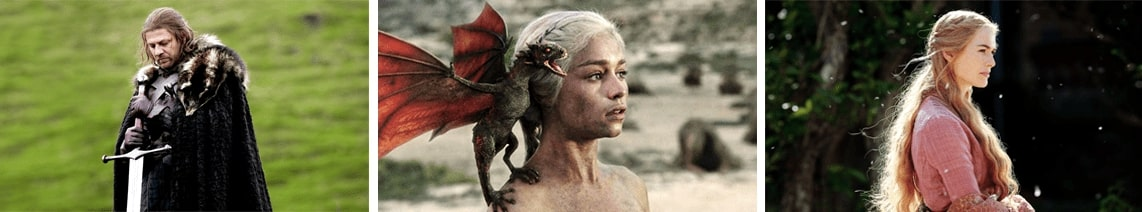
\includegraphics[width=0.48\textwidth]{img/s1/frames_s1.jpg}
\end{figure}


\subsubsection{General Network Properties}

The first season of Game of Thrones is composed of 126 nodes and 549 edges, with a graph density of 0.697, and is a connected graph with no isolated nodes.

\paragraph{Small World Network:} Season 1 resulted to be of the family of small world network. This is supported by values found for $\lambda=1$ and $\gamma=10.2$.

\paragraph{Diameter and Shortest Path:}

The diameter is 6, which is a low value, suggesting that the nodes are very connected to each other. This suggests that is easy to create connections between characters. The path beween most distant nodes involves the following characters: \textit{['Irogenia', 'Doreah'], ['Doreah', 'Daenerys'], ['Daenerys', 'Ned'], ['Ned', 'Jon'], ['Jon', 'Sam'], ['Sam', 'Melessa']}. Irogenia is mentioned by the handmaid Doreah while talking to Daenerys Targaryen. Ned Stark is linked to Daenerys only because of a discussion he had with the king, Robert Baratheon, about the latter's choice of sending an assassin to murder her. Jon is, apparently, Ned's illegitimate son, Sam is Jon's best friend, and Melessa is Sam's mother.
To justify the low diameter we find the average shortest path to be 2.64, which is fairly good result being a bit more than half of the diameter path. This confirms that the graph is well connected, even though the density is low.

\begin{figure}[!h]
    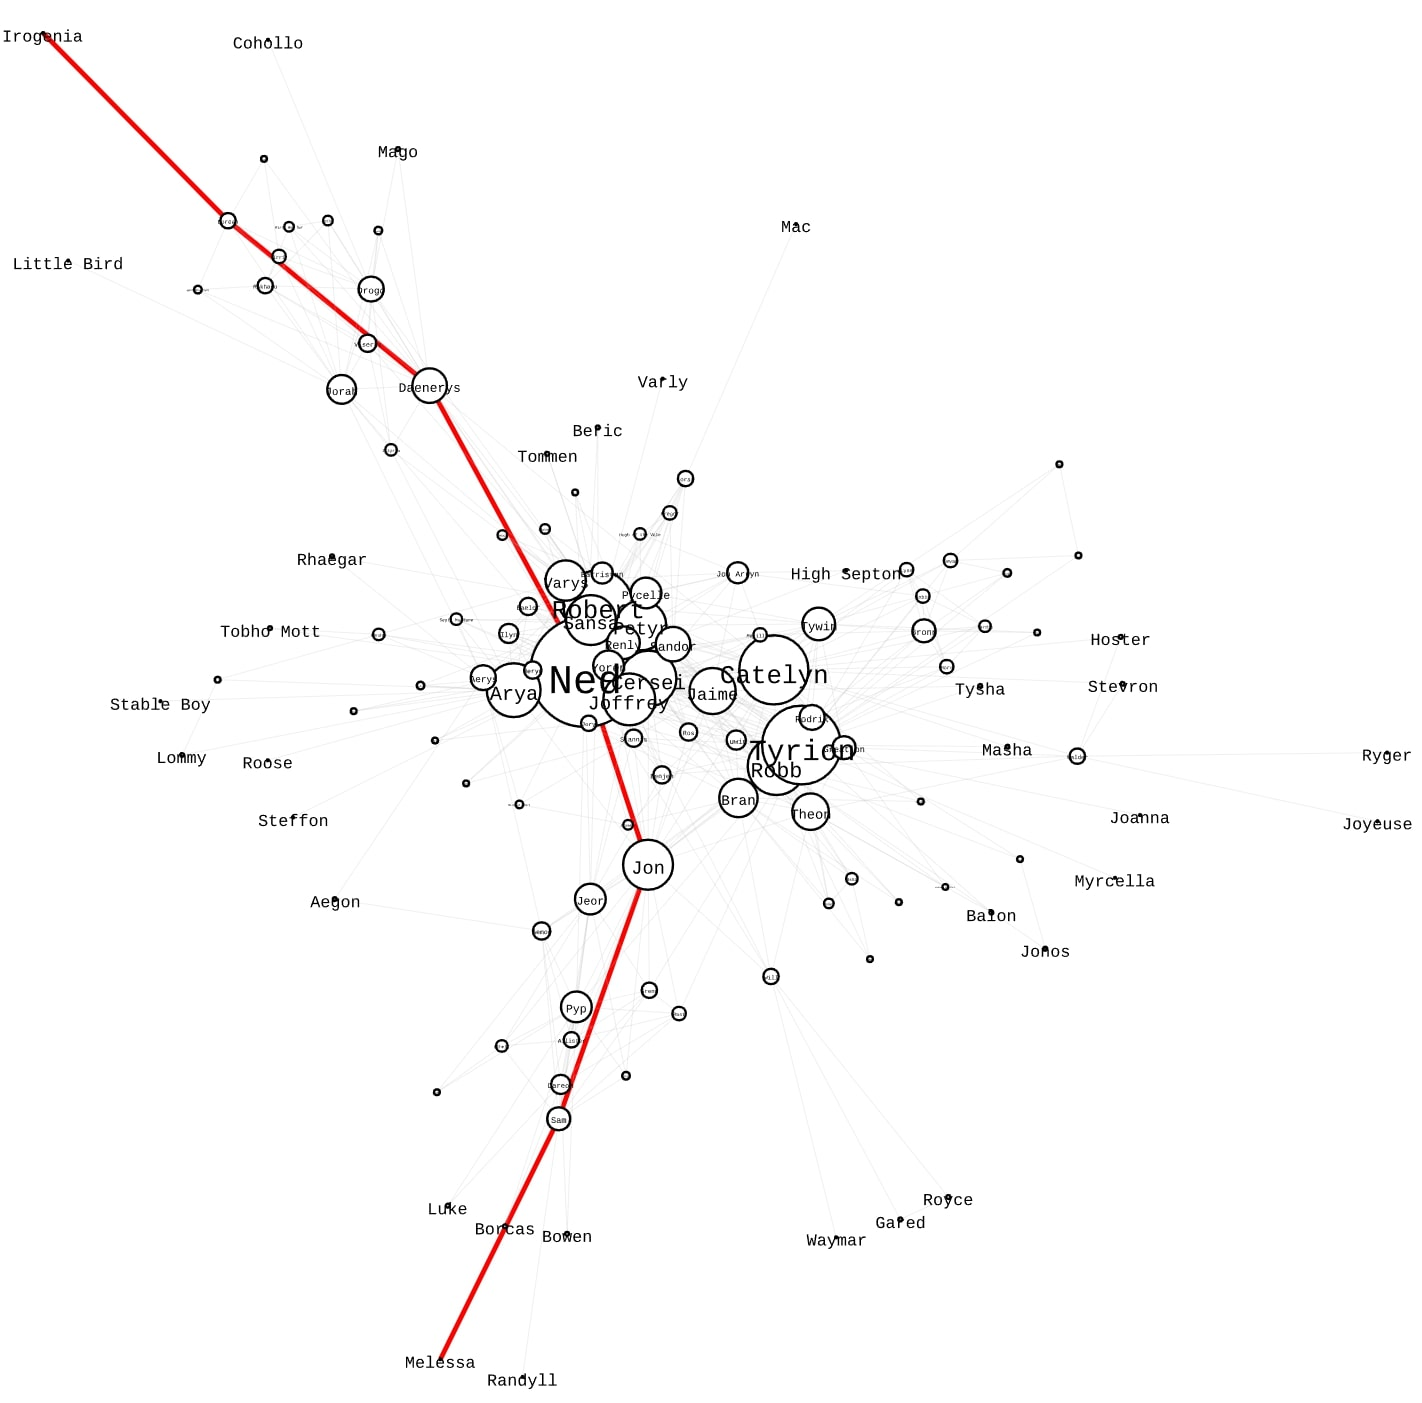
\includegraphics[width=0.35\textwidth]{img/s1/diameter_path.jpg} \\
    \caption{\small{Diameter path of Season 1}}
\end{figure}

\paragraph{Degree:}

The average degree is 8.714, while the minimum is 1, belonging to characters such as Randyll, Myrcella, Waymar and Irogenia, which are secondary characters. However, by calculating the average degree of node's neighbours, it is strikingly clear that Myrcella is part of an important family, as the value is 41. Notably, this value is much higher than any of the characters with highest degree. 
The highest degree is 57, belonging to Ned Stark, who has a central importance in this season, followed by Tyrion Lannister and Robert Baratheon, which are also physically close for the majority of the season, both in Winterfell and King's Landing. The mean is index that there are more characters which have a low degree. Indeed, the most frequent degree is 2 with 18 nodes. The degree distribution is appreciable in the plots\textsuperscript{\ref{fig:degplot_s1}} below, as well as the table\textsuperscript{\ref{tab:deg_s1}} with the 10 nodes with highest degree.

\begin{figure}[!h]
    \centering
    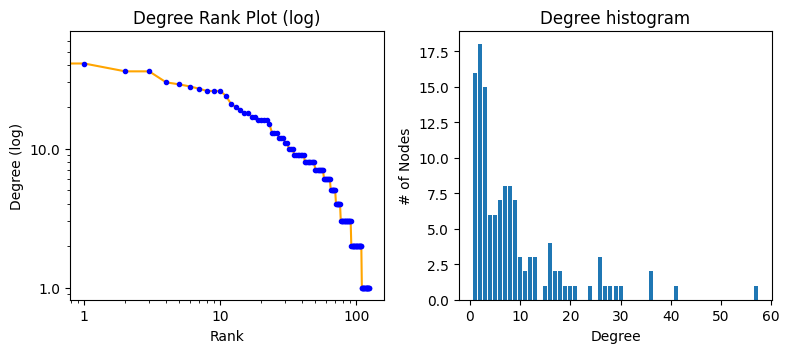
\includegraphics[width=0.5\textwidth]{img/s1/degree_plot.jpg}
    \caption{\small{Degree distribution of Season 1}}
    \label{fig:degplot_s1}
\end{figure}

\begin{table}[!h]
    \centering
    \small
    \begin{tabular}{c|c|c}
        Node & Degree & \small{Avg. Deg. of Neighbours}  \\
        \hline
         Ned  &  57 & 13.2 \\
         Tyrion & 41 & 14.7 \\
        Robert & 36 & 17.3 \\
        Catelyn  & 36 & 17.0 \\
        Robb  & 30 & 17.7 \\
        Cersei  & 29 & 20.1 \\
        Arya  & 28 & 18.4 \\
        Joffrey  & 27 & 20.2 \\
        Petyr  & 26 & 18.9 \\
        Jon  & 26 & 18.7 \\
        \hline 
    \end{tabular} \\
    \caption{Top 10 nodes with highest degree}
    \label{tab:deg_s1}
\end{table}



\paragraph{Bridges:}

The network has 16 bridges, as it is possible to see from the visualization below:

\begin{figure}[!h]
\centering
    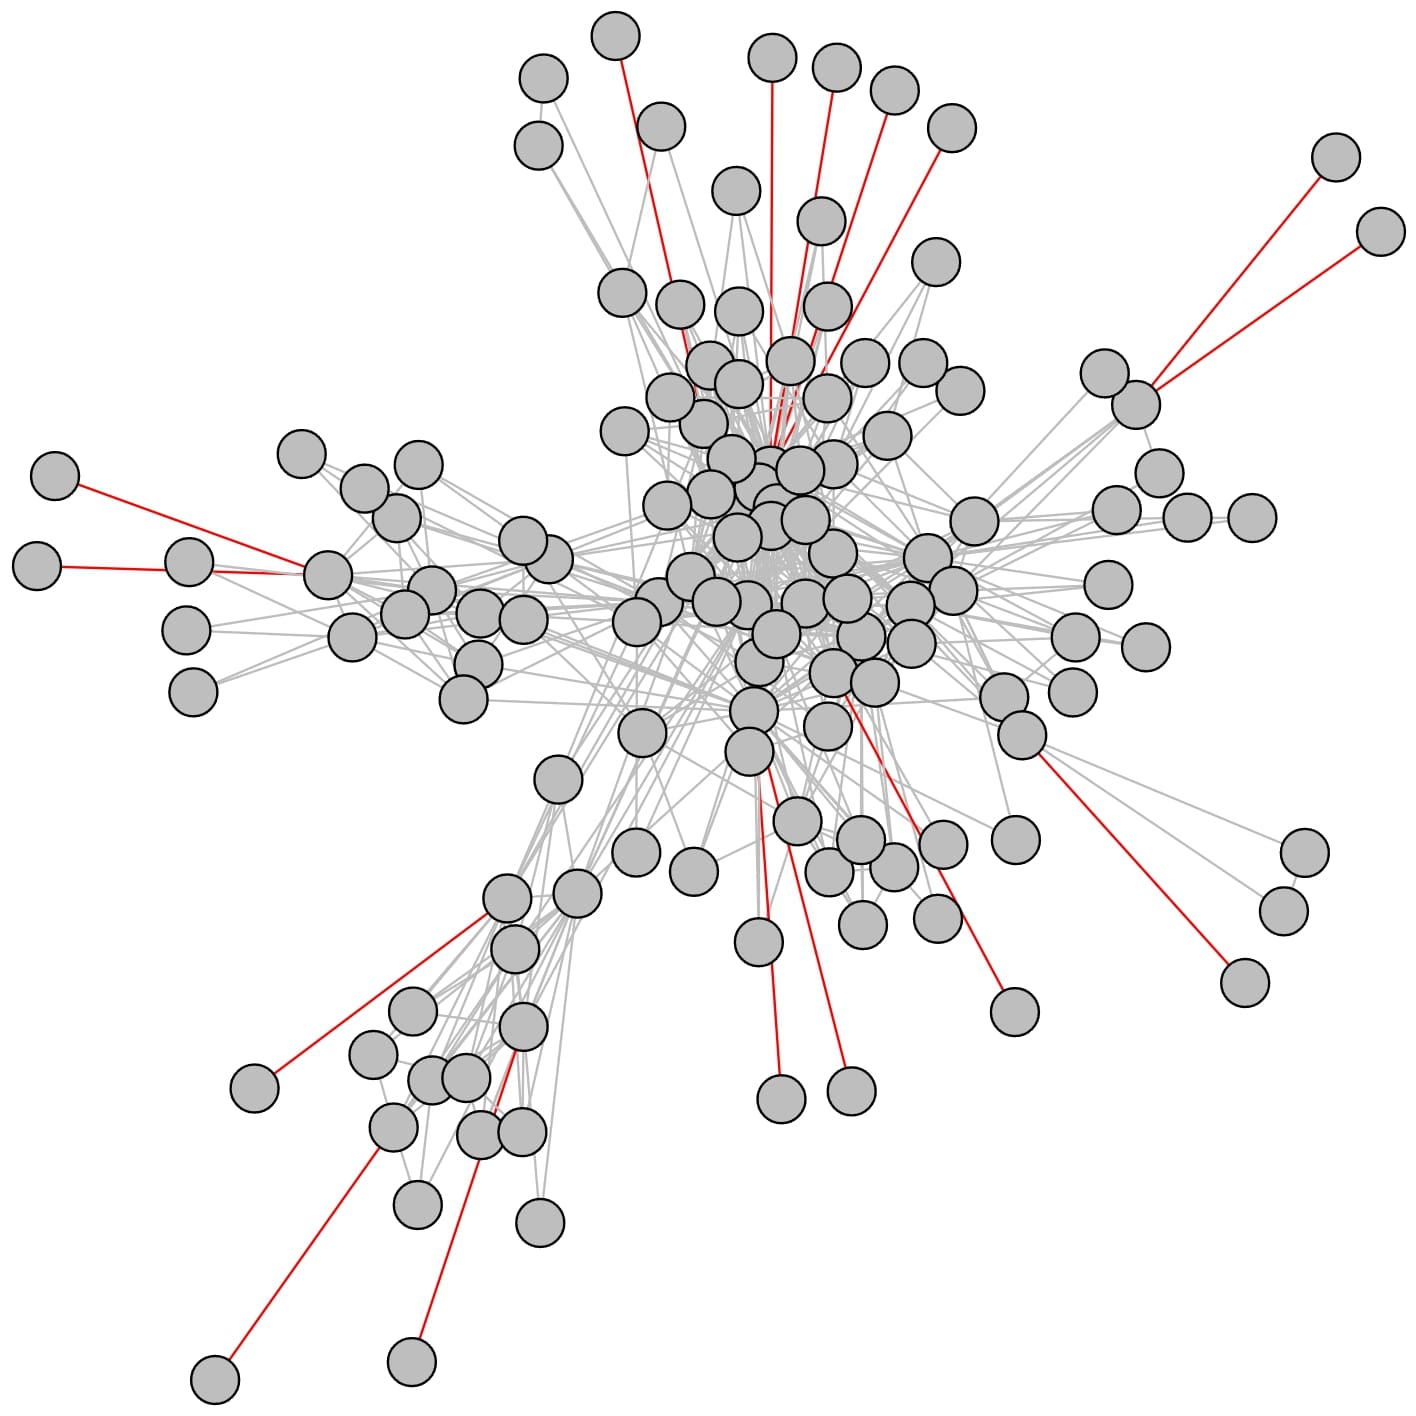
\includegraphics[width=0.3\textwidth]{img/s1/bridges.jpg}
\end{figure}

They involve \textit{('Ned', 'High Septon'), ('Ned', 'Roose'), ('Ned', 'Steffon'), ('Ned', 'Varly'), ('Jorah', 'Little Bird'), ('Sam', 'Melessa'), ('Sam', 'Randyll'), ('Drogo', 'Cohollo'), ('Arya', 'Stable Boy'), ('Tyrion', 'Myrcella'), ('Tyrion', 'Joanna'), ('Loras', 'Mac'), ('Walder', 'Ryger'), ('Walder', 'Joyeuse'), ('Doreah', 'Irogenia'), ('Will', 'Waymar')}.

The fact that Ned Stark and Tyrion Lannister are involved in multiple bridges suggests that thet are central figures whose interactions are critical for maintaining the cohesion of the network. Interestingly, Sam's connections with Melessa and Randyll (his mother and father) as bridges highlight the potential fragility of his familial ties.

\subsubsection{Centrality}

For a better first visualization of the network, below we plot Season 1's interaction network\textsuperscript{\ref{fig:pr_s1}} where the node sizes are scaled according to PageRank centrality, and the layout is computed using the Fruchterman-Reingold force-directed layout algorithm.

\begin{figure}[!h]
    \centering
    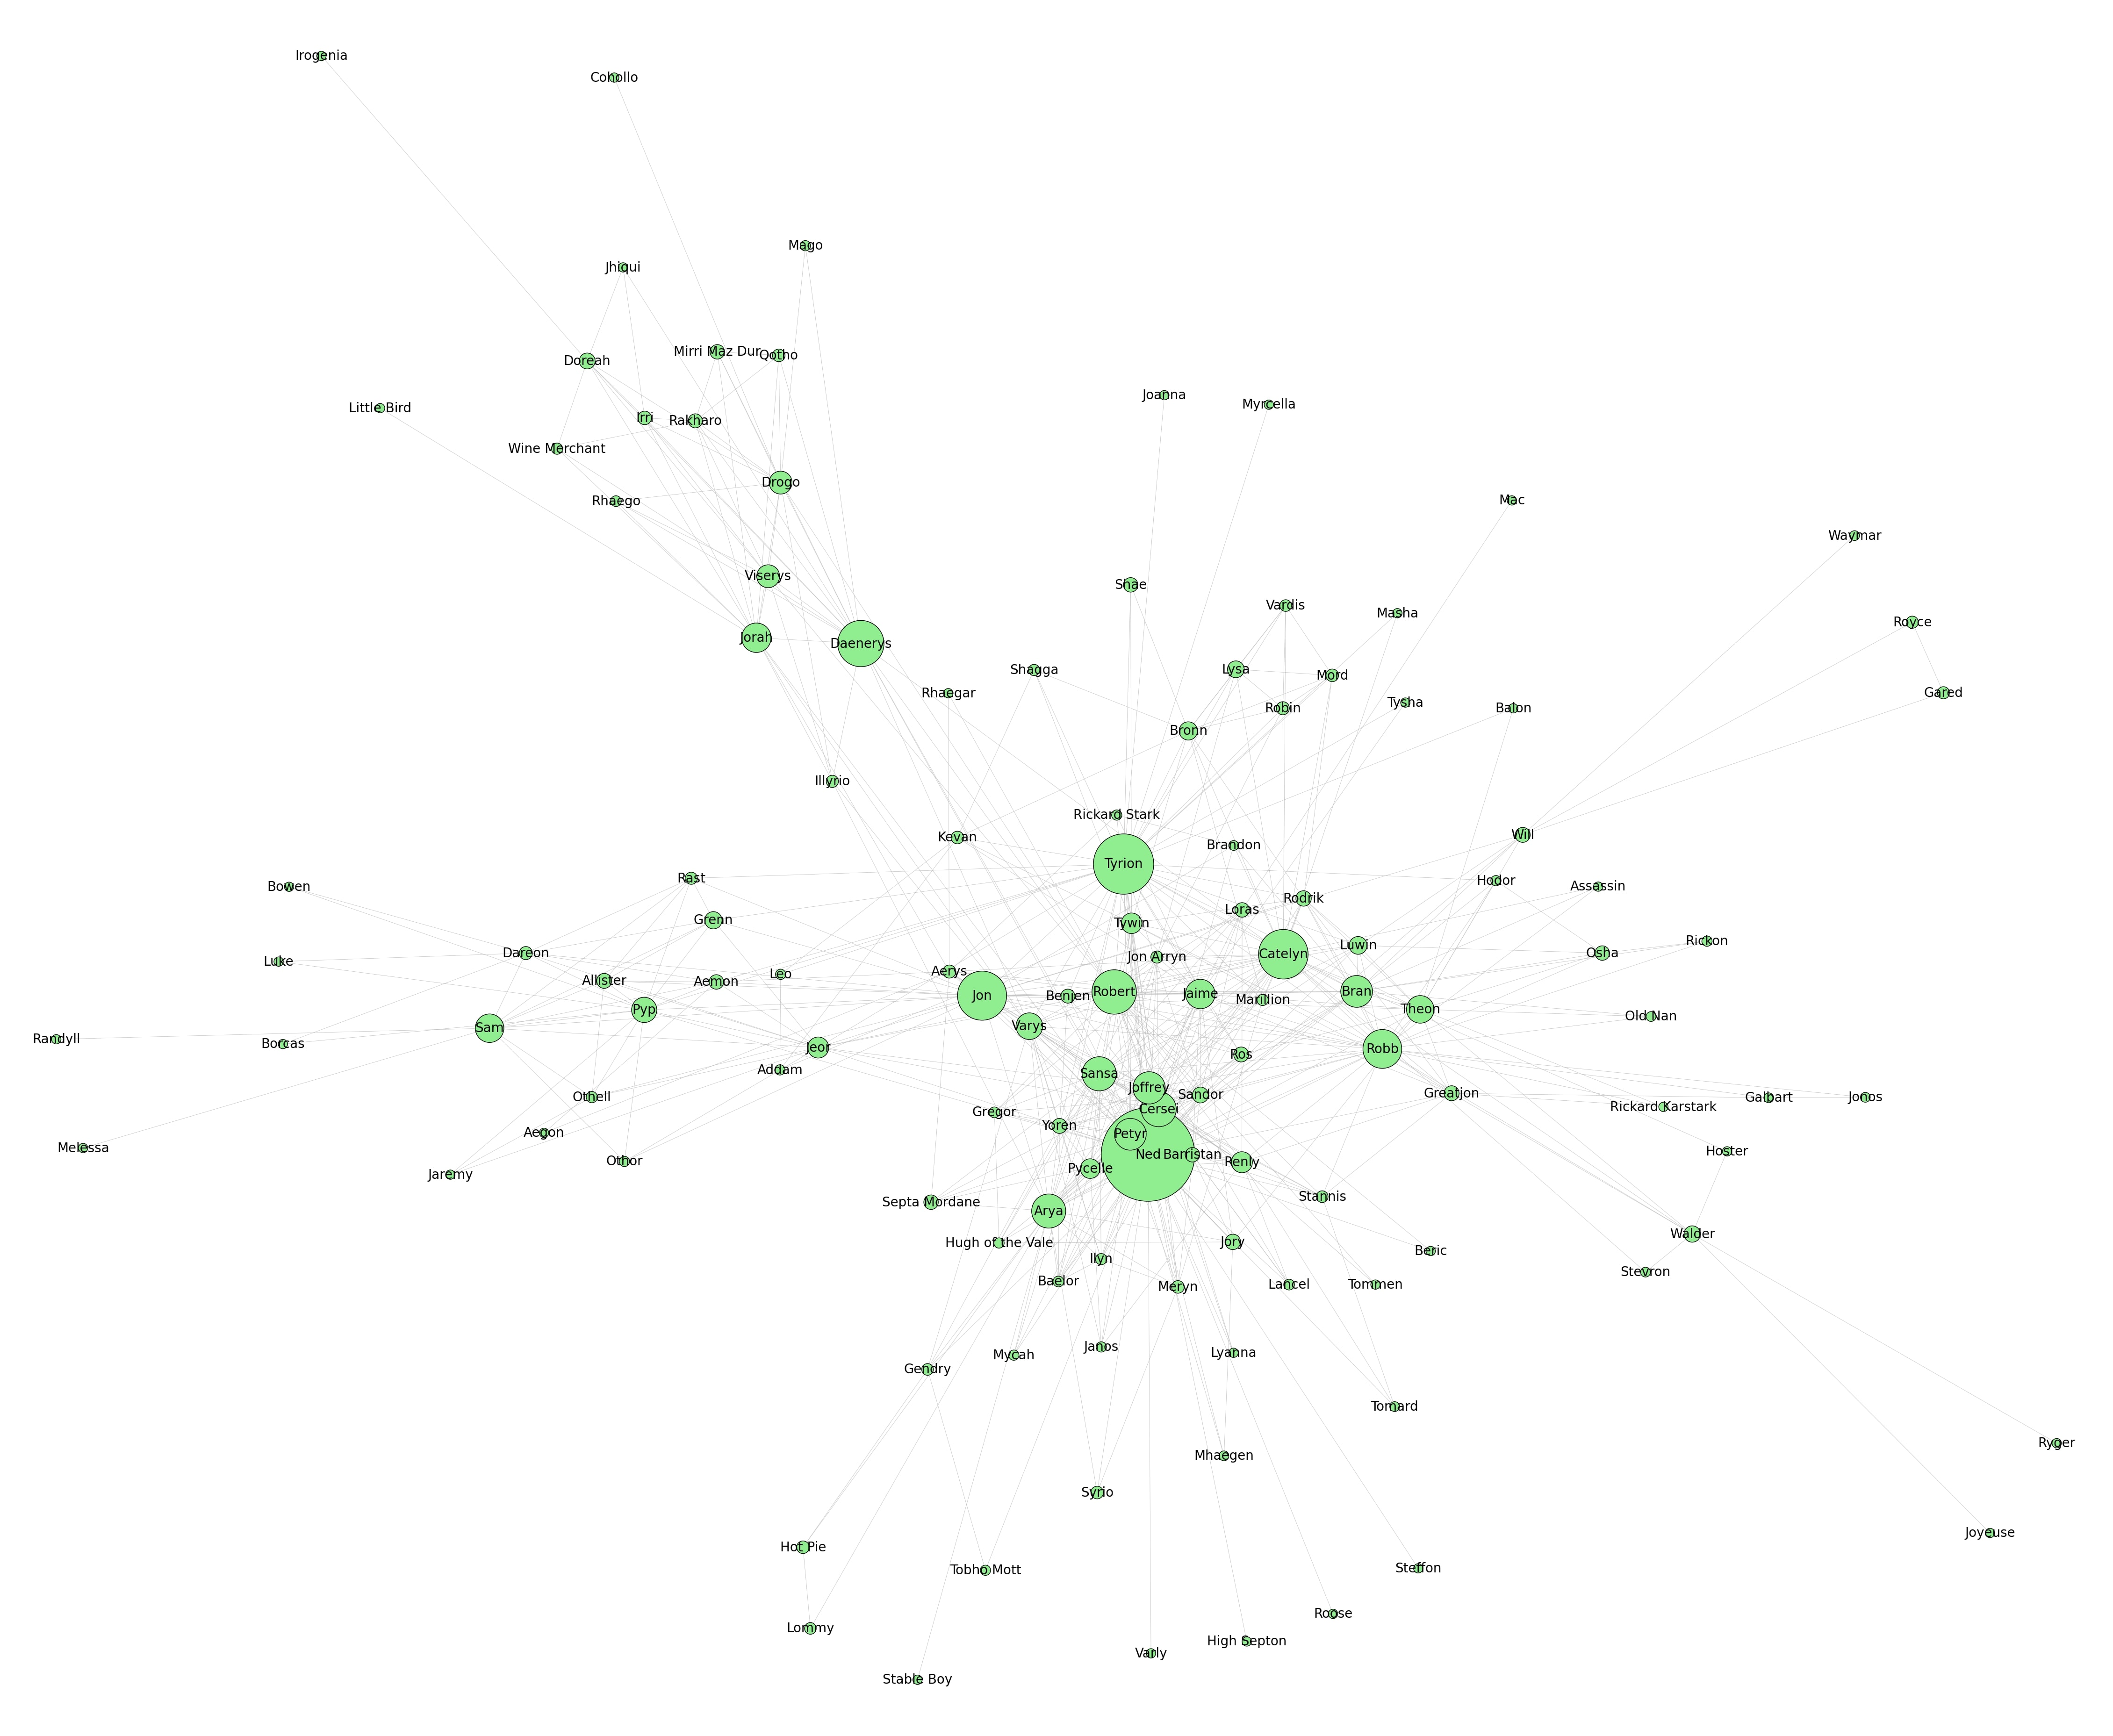
\includegraphics[width=0.5\textwidth]{img/s1/pagerank_network.jpg}
    \label{fig:pr_s1}
\end{figure}


The following tables\textsuperscript{\ref{tab:cent_s1},\ref{tab:mcent_s1}} report the results obtained by the different centrality measures. In particular, the first table displays the first 5 characters of the network with the highest centrality score, for each type of centrality. As it is possible to notice, regardless of the centrality type, the first five nodes are mostly the same ones. In particular, Ned is the top character for every type of centrality, which makes sense since he is the Hand of the King, therefore is a central figure connecting various characters and political factions; moreover a lot of of the action of the first season revolve around the facts that lead to his execution. Similarly, Tyrion's role as a mediator and advisor places him in strategic positions where he influences many events and connects disparate groups. Robert, being the king, is obviously a central figure in various aspects, which are all captured by the different centrality measures. 



\begin{table}[!h]
    \centering
    \small
    \begin{tabular}{c|c|c}
        Measure & Character & \small{Highest Centrality Score} \\
        \hline
                    & Ned & 0.303 \\
                    & Tyrion & 0.163 \\
        Betweenness & Catelyn & 0.118 \\
                    & Robert & 0.110 \\
                    & Daenerys & 0.101 \\
        \hline 
                    & Ned & 0.628 \\
                    & Robert & 0.553 \\
        Closeness   & Catelyn & 0.551 \\
                    & Tyrion & 0.543 \\
                    & Jon & 0.519 \\
        \hline 
                    & Ned & 0.315 \\
                    & Robert & 0.248 \\
        Eigenvector & Catelyn & 0.239 \\
                    & Tyrion & 0.230 \\
                    & Jon & 0.229 \\
        \hline 
                    & Ned & 0.011 \\
                    & Tyrion & 0.013 \\
        Harmonic    & Robert & 0.013 \\
                    & Catelyn & 0.013 \\
                    & Robb & 0.014 \\
        \hline
                    & Ned & 0.456 \\
                    & Tyrion & 0.328 \\
        Degree      & Robert & 0.288 \\
                    & Catelyn & 0.288 \\
                    & Robb & 0.240 \\
        \hline
                    & Ned & 1.000 \\
                    & Tyrion & 0.550 \\
        Weighted Degree & Catelyn & 0.453 \\
                    & Robert & 0.436 \\
                    & Daenerys & 0.415 \\
        \hline
                    & Ned & 0.047 \\
                    & Tyrion & 0.034 \\
        PageRank    & Catelyn & 0.029 \\
                    & Robert & 0.028 \\
                    & Robb & 0.024 \\
        \hline
    \end{tabular}
    \vspace{0.2cm}
    \caption{Top characters with highest centrality scores}
    \label{tab:cent_s1}
\end{table}






\begin{table}[!h]
    \centering
    \small
    \begin{tabular}{c|c}
        Centrality Measure & Mean  \\
        \hline
        Betweenness & 0.013 \\
        Closeness & 0.389 \\
        Eigenvector & 0.059 \\
        Harmonic & 0.018 \\
        Degree & 0.069 \\
        Weighted Degree & 0.083 \\
        PageRank & 0.008 \\
        \hline 
    \end{tabular} \\
    \caption{Centrality means of Season 1}
    \label{tab:mcent_s1}
\end{table}

From the two tables \textsuperscript{\ref{tab:cent_s1} , \ref{tab:mcent_s1}}, it is possible to notice the scores about the top five characters of the betweenness, closeness, eigenvector and degree centrality are much higher than the respective means. On
the contrary, the scores for the top five characters of the harmonic centrality is very near to the mean.

\subsubsection{Homophily}



\paragraph{Assortativity}

The degree assortativity coefficient is -0.141, which is negative, indicating that characters who have high-weighted connections (i.e. frequent interactions) tend to connect to characters with low-weighted connections, and vice versa. This makes sense since prominent characters are likely to interact with less important characters, reflecting hierarchical and political dynamics. The same is true for less prominent characters, which might work for or are affiliated with important ones, like members of the royal family.

\paragraph{Jaccard Similarity}

In the table\textsuperscript{\ref{tab:jac_s1}} below, the first five Jaccard similarity scores between every couple of nodes are reported: \\

\begin{table}[!h]
    \centering
    \small
    \begin{tabular}{c|c|c}
        First Node & Second Node & \small{Jaccard Similarity Score}  \\
        \hline
        Lysa Arryn & Robin Arryn & 0.75 \\
        Grenn & Rast & 0.66 \\
        Mirri Maz Duur & Qotho & 0.66 \\
        Robin Arryn & Vardis Egen & 0.625 \\
        Lysa Arryn & Vardis Egen & 0.625 \\     
        \hline 
    \end{tabular} \\
    \caption{Top 5 characters for Jaccard Similarity Score}
    \label{tab:jac_s1}
\end{table}

These findings make sense considering the family relationships and overall plot of the story. Most of the characters are part of the Arryn family or affiliated with it. Robin is Lysa's son ($weight_{r,l}=30)$, which is consistent with their highest score. Vardis Egen served Jon Arryn, Lysa's husband, as his captain of the guards and he is chosen as the champion for House Arryn by Lysa when Tyrion demands a trial by combat to demonstrate his innocence in the death of Lord Jon Arryn. 
However, there are exceptions: Quotho is one of Drogo's bloodriders, and objects to the Lhazareen godswife Mirri Maz Duur treating a small wound Drogo takes, calling her a witch; therefore, they are both part of the Dothraki story line. Finally, Grenn and Rast are both part of the Night's Watch.


\subsubsection{Triangles}

In this network, there are 1254 triangles. The ten characters with most triangles are
Ned (280), Robert (185), Cersei (181), Catelyn	(180), Tyrion (175), Joffrey (152), Robb (142), Littlefinger (139), Sansa (137), Arya (136). This makes sense since all of these characters are part either of the Stark's family and/or the community of King's Landing, which in this season heavily interact.

One of the most distinctive features of this network is how tightly concentrated the action is. There are strong triangles in each community\textsuperscript{\ref{fig:tr_s1}}.

\begin{figure}[!h]
    \centering
    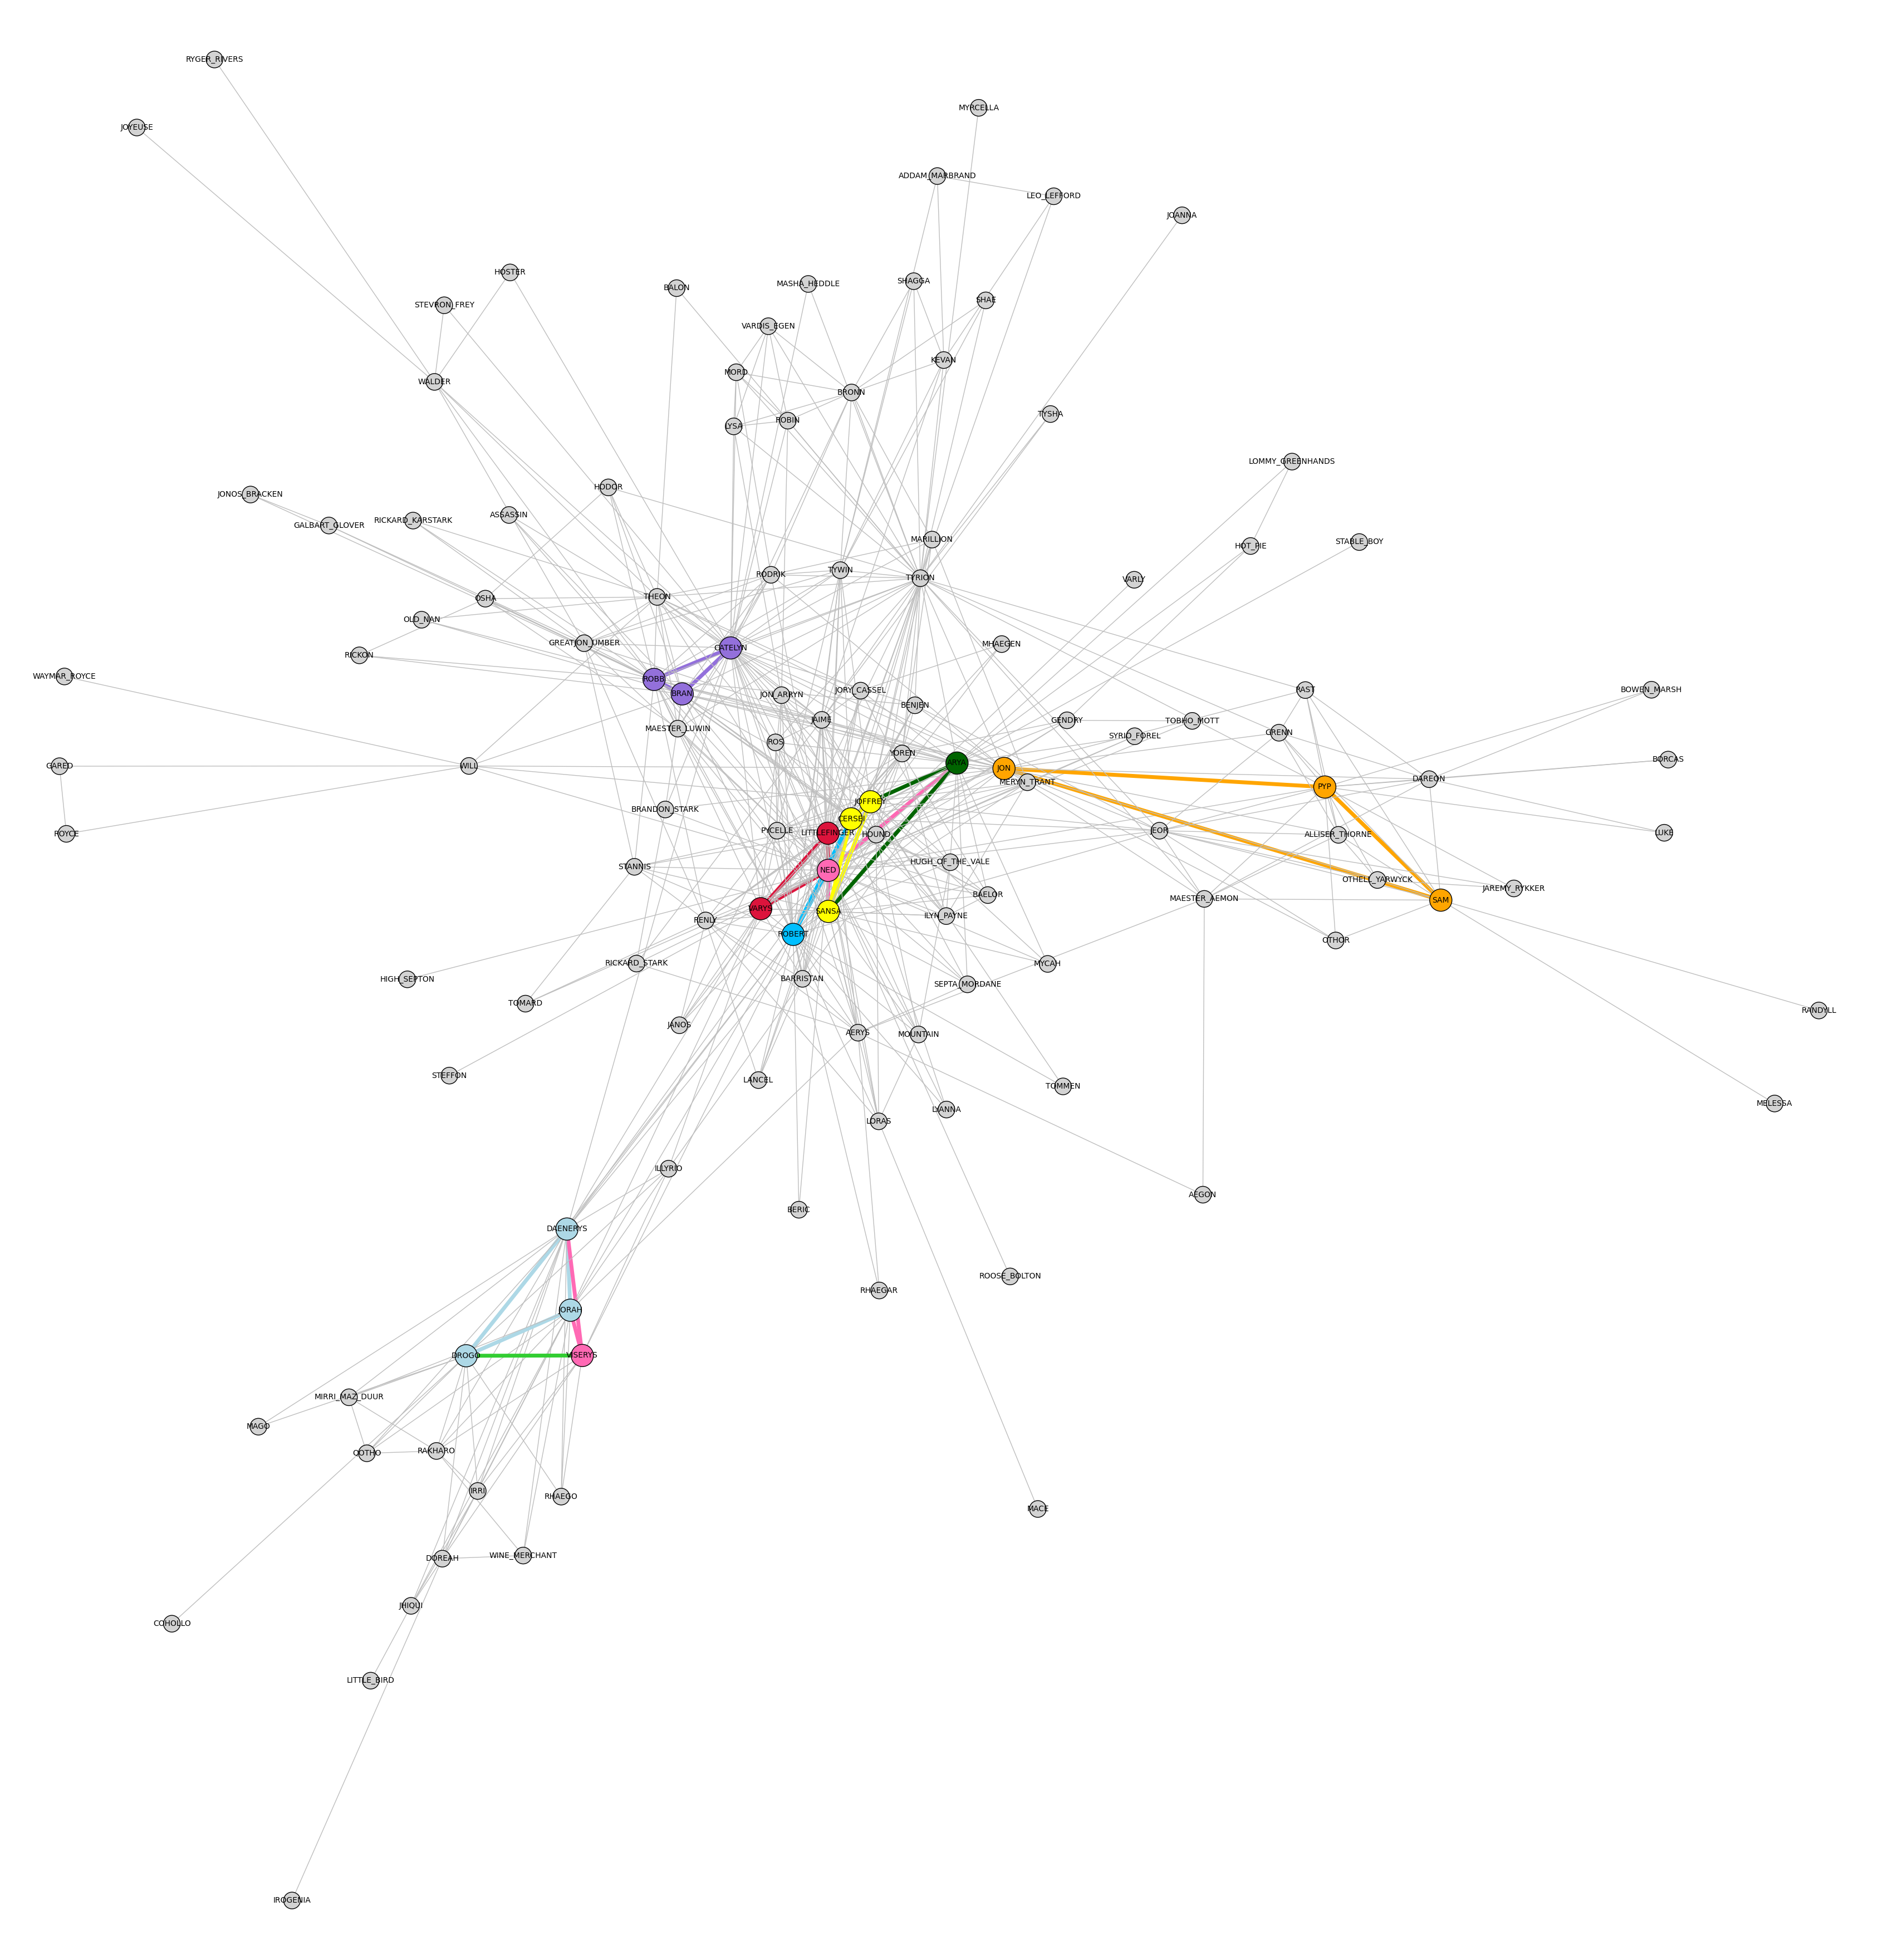
\includegraphics[width=0.4\textwidth]{img/s1/s1_triangles.jpg}
    \caption{\small{Noteworthy triangles in the graph}}
    \label{fig:tr_s1}
\end{figure}

In the table\textsuperscript{\ref{tab:tr_s1}} below, selected triangles deemed to be interesting from a narrative stand-point are presented, taking into consideration the overall strength of the triangle (weights represent number of interactions) and the strongest edge in it. 


\begin{table}[!h]
    \centering
    \small
    \begin{tabular}{c|c|c}
        Triangle & Strength & Strongest Edge  \\
        \hline
        \small{(Ned, Robert, Cersei)} & 358 & 192 \small{(Ned, Robert)} \\
        \small{(Ned, Littlefinger, Varys)} & 276 & 107 \small{(Ned, Littlefinger)}\\
        \small{(Ned, Arya, Sansa)} & 192 & 90 \small{(Ned, Arya)}\\
        \small{(Arya, Joffrey, Sansa)} & 146 & 69 \small{(Joffrey, Sansa)}\\
        \small{(Cersei, Joffrey, Sansa)} & 159 & 69 \small{(Joffrey, Sansa)}\\
        \small{(Catelyn, Robb, Bran)} & 166 & 90 \small{(Catelyn, Robb)}\\
        \small{(Jon, Sam, Pyp)} & 193 & 121 \small{(Jon, Sam)} \\
        \small{(Daenerys, Drogo, Viserys)} & 184 & 91 \small{(Daenerys, Drogo)}\\
        \small{(Daenerys, Jorah, Viserys)} & 263 & 154 \small{(Daenerys, Jorah)}\\
        \small{(Daenerys, Jorah, Drogo)} & 265 & 154 \small{(Daenerys, Jorah)}\\
        \hline 
    \end{tabular} \\
    \caption{\small{Strength of interesting triangles}}
    \label{tab:tr_s1}
\end{table}

Ned is part of many triangles, some completely friendly - e.g with his daughters Sansa and Arya, with whom is very close ($weight_{n,s}=49$), ($weight_{n,a}=90$) -, others where there is an enemy - Cersei is Robert's wife, but she is hostile to Ned ($weight_{n,c}=86$) -, and finally one where Ned interacts with potential enemies; in fact, it will be Littlefinger to betray him ($weight_{n,l}=107$). Sansa interacts a lot with Joffrey ($weight_{s,j}=69$), being unfortunately promised to being his spouse, even compared to Joffrey's bond with her mother. This triangle really impacts Sansa, who realizes that, after all, being a princess to Joffrey feels more like hell rather than a fairy tale.
Noteworthily, Catelyn interacts with her sons Robb and Bran: at first glance, it seems that Catelyn is closer to Robb ($weight_{c,r}=90$) than to Bran ($weight_{c,b}=28$). However, the Catelyn-Bran edge weight would be higher if Bran was not comatose and could talk. Actually, Catelyn spends most of the time with Bran, but as we already said, the network prioritizes dialogues over actions.
Jon, at the Wall, interacts with Sam and Pyp, and Sam is his best friend, which is supported by the strongest edge.
Daenerys is obviously close to his husband Drogo ($weight_{da,dr}=91$), but is consistently closer to his advisor Jorah ($weight_{d,j}=154$), who is also secretly in love with her.

It is also interesting to investigate triangles of specific characters, for example Tyrion.

\begin{figure}[!h]
    \centering
    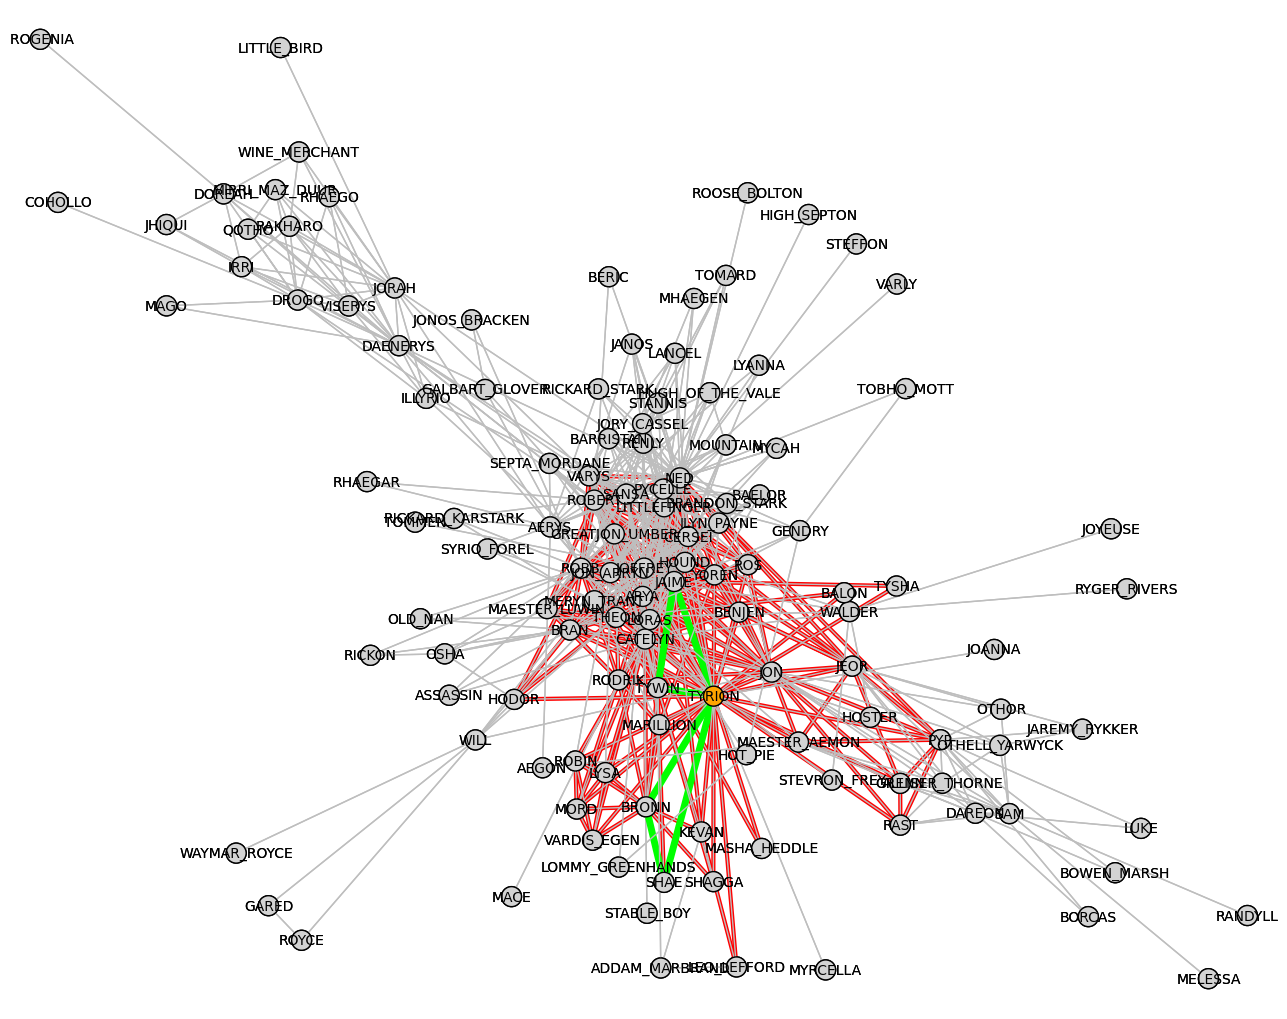
\includegraphics[width=0.45\textwidth]{img/s1/triangles_tyrion.jpg}
    \caption{\small{Triangles involving Tyrion. Triangles connecting him to House Lannister and allies are highlighted in green.}}
\end{figure}

Tyrion's community is looser, already from the first season, and captures his independent spirit. Moreover, he is part of triangles with Tywin and Jamie, and with Bronn and Shae. The former triangle captures his ties to House Lannister, the seat of his power and station. The latter is the motley pair of allies that he develops during his misfortunes.

We can compare this with another character, Varys, which is a spy working for the Lannisters and Baratheons in King's Landing. From the graph below it is clear how in the first season, other than interacting with people in King's Landing, his focus is devoted to gather information about Daenerys. 

\begin{figure}[!h]
    \centering
    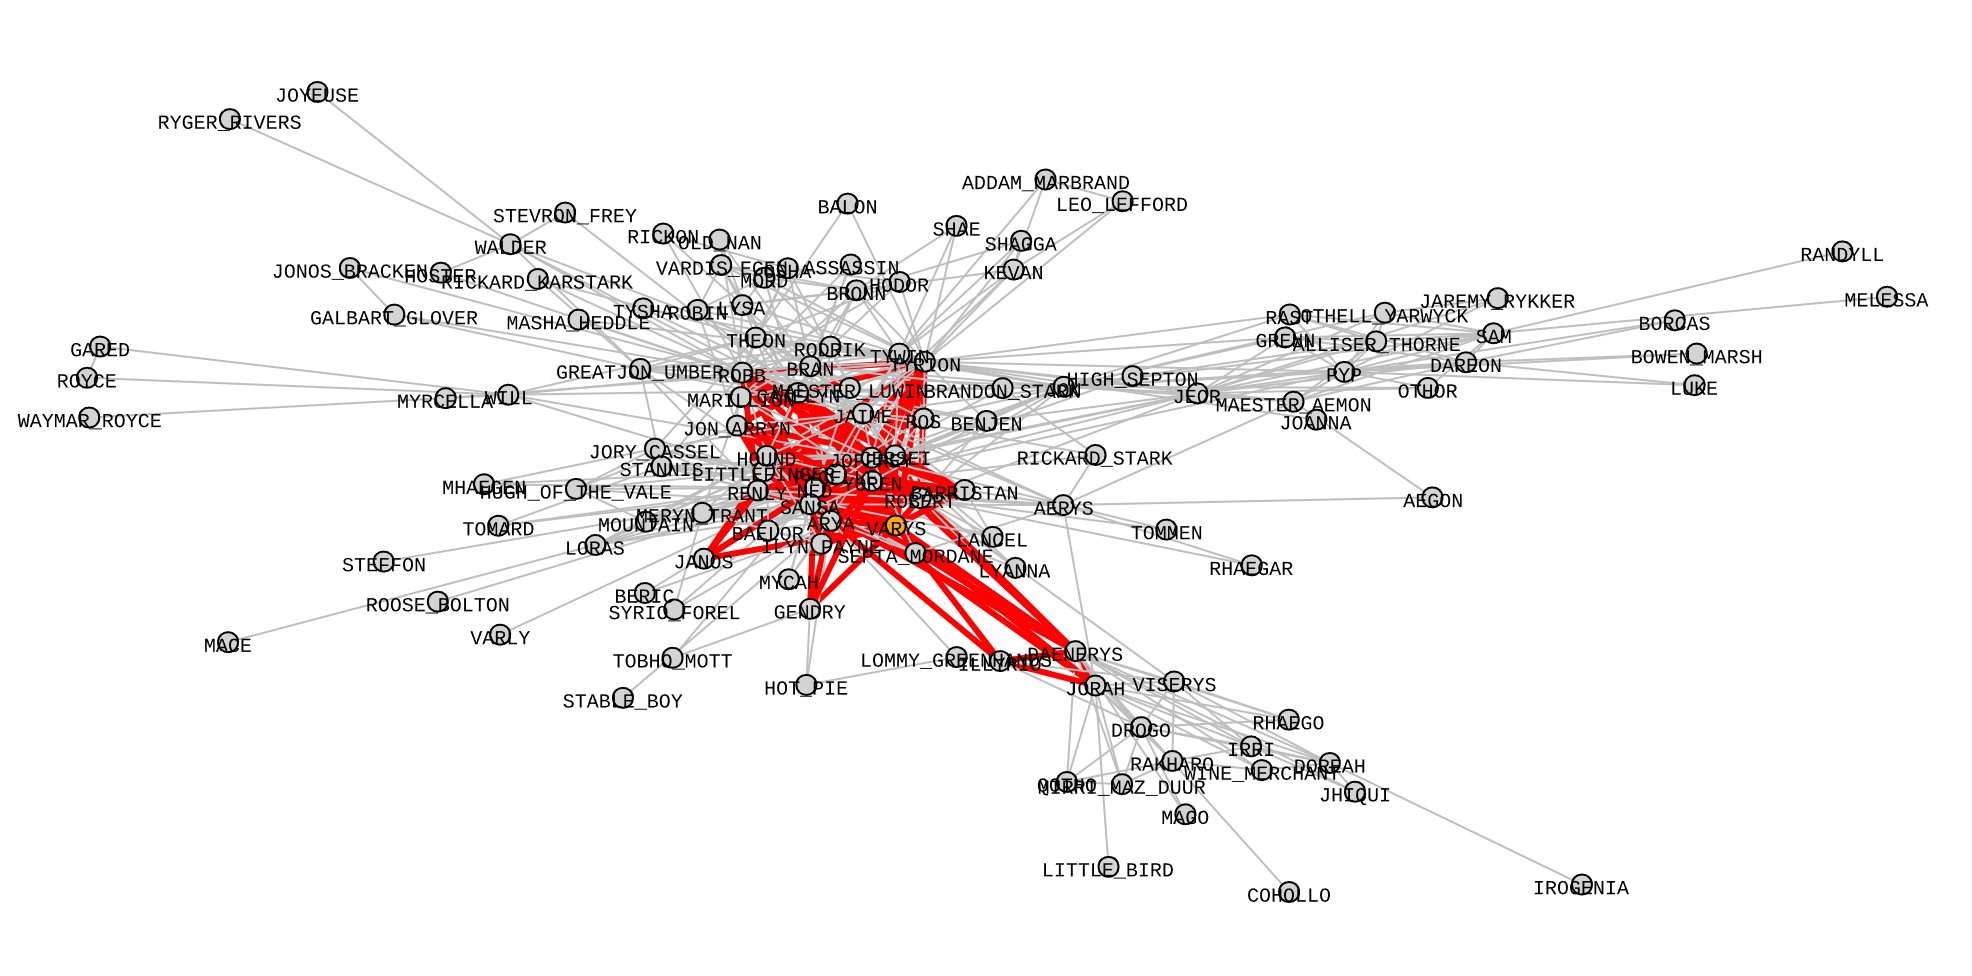
\includegraphics[width=0.5\textwidth]{img/s1/triangles_varys.jpg}
    \caption{\small{Triangles involving Varys.}}
\end{figure}

\subsubsection{Clustering Coefficients}

The Global clustering coefficient for season 1 is 0.383, Average clustering coefficient is 0.629.

\subsubsection{Community Detection}

As mentioned before, the aim is to identify major communities of interacting characters. It is unfortunately not possible to isolate allies and enemies, as the network lacks signed edges.

\paragraph{Infomap} The Modularity score for Infomap is 0.448. The algorithm is able to identify important communities that are consistent with the main plot lines of Game of Thrones' first season. 

\begin{figure}[!h]
    \centering
    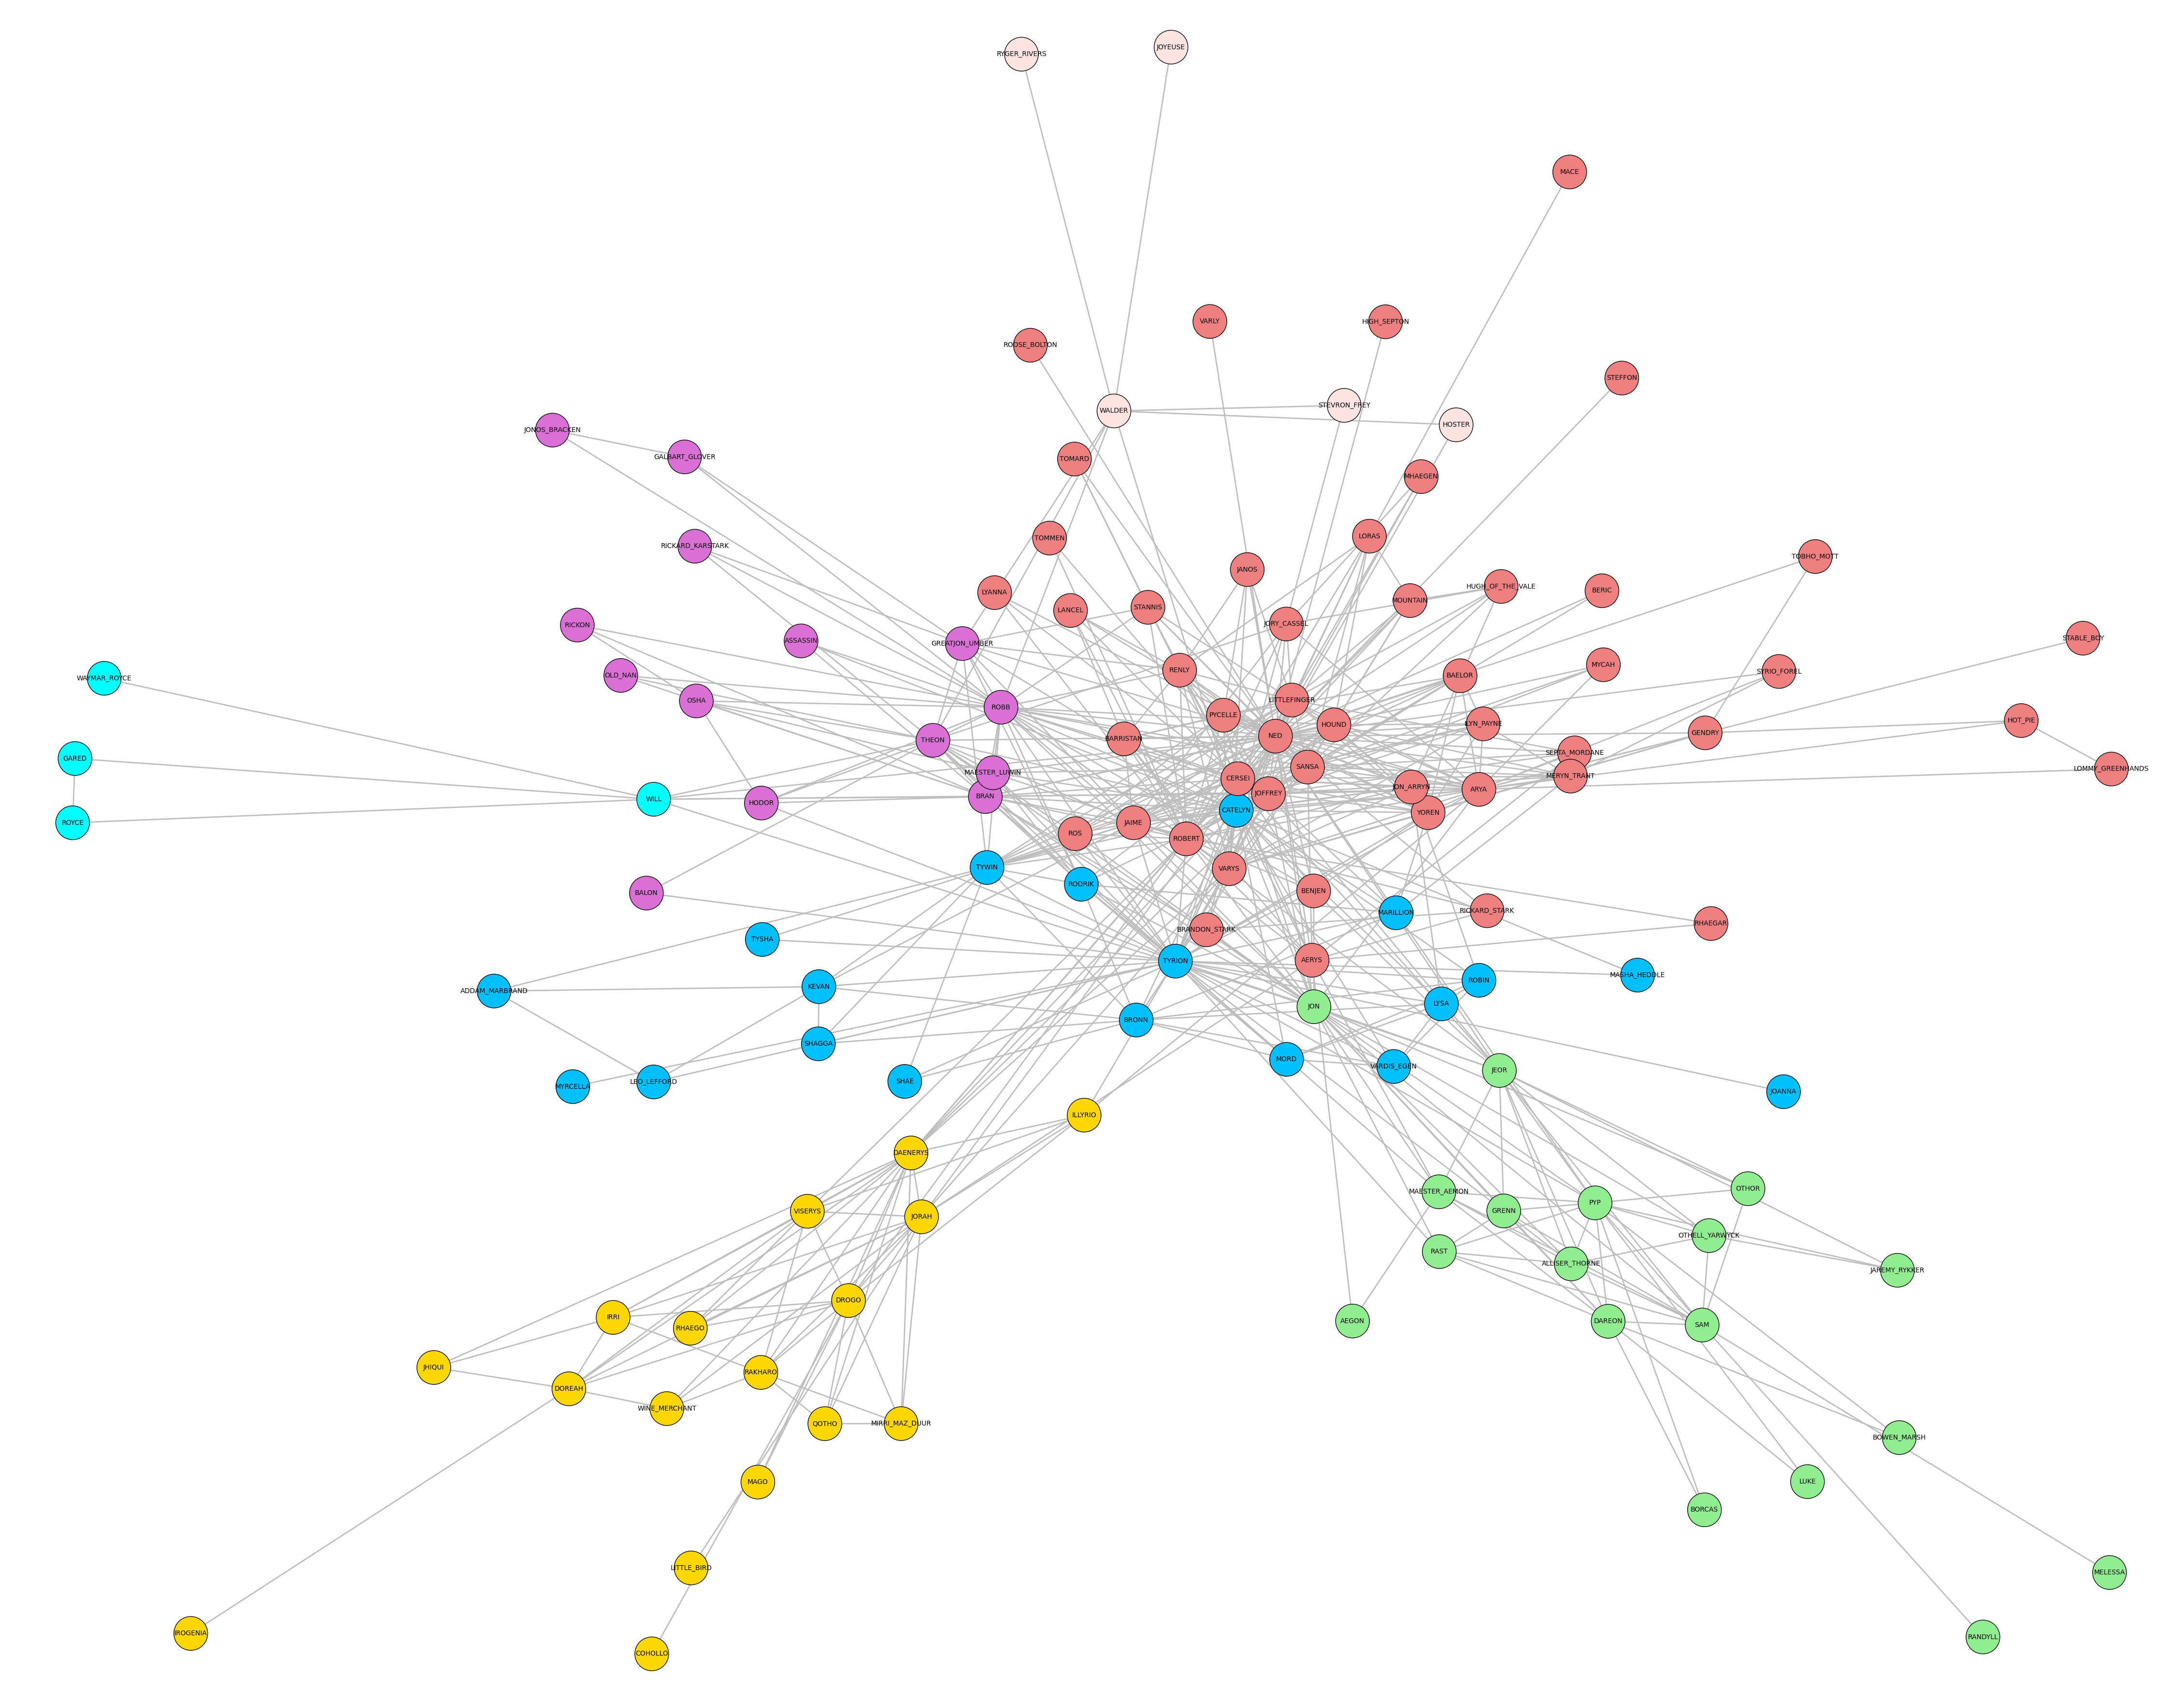
\includegraphics[width=0.5\textwidth]{img/s1/communities_infomap.jpg}
    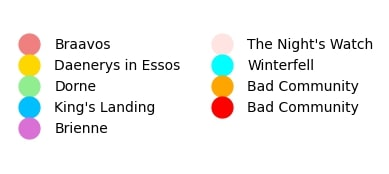
\includegraphics[width=0.4\textwidth]{img/s1/infomap_legend.jpg} \\
    \vspace{0.2cm}
    \label{fig:infomap_s1}
    \caption{\small{Community detection using Infomap}}
\end{figure}

In particular, the following communities are recognizable:

\begin{itemize}
    \item \textbf{King's Landing} (Ned, Robert, Littlefinger): we can clearly see the community mainly composed by the people in King's Landing, where major events of the first season take place. Notably, king Robert dies after suffering a hunting accident, and delegates Ned to be king until Jeoffrey comes to age. However, Littlefinger betrays Ned and gets him executed. 
    \item \textbf{The Dothraki} (Daenerys, Jorah, Drogo): we can clearly see the community that forms from the wedding of Daenerys and Drogo. Daenerys is tightly linked to her brother Viserys ($weight_{d,v}=66$), the merchant Hilyrio, who gifts her three dragon eggs, and of course to Drogo, who in turn is more linked to people from his khalasar.
    \item \textbf{The Starks} (Robb, Theon, Bran): this is the community comprising the family of the Starks, as well as other characters they interact with. Notably, there is a strong bond between Bran and Maester Luwin ($weight_{b,l}=53$), as Bran is left in a coma after a fall and Maester Luwin takes care of him. It is interesting how Infomap did not recognize Bran's mother, Catelyn, as part of the Stark's community, placing her in the community of the Lannisters, even if she spends most of the time watching over Bran, also fighting against an assassin sent to kill her son.
    \item \textbf{Tyrion vs Catelyn} (Tyrion, Bronn, Catelyn): they are the protagonists of the first clash of Game of Thrones. Catelyn is convinced that Tyrion is the instigator of the attempted murder of Bran. So she kidnaps Tyrion and brings him to trial ($weight_{t,c}=41$), although Tyrion wins thanks to his squire Bronn. Catelyn's obsession for having justice is likely why Infomap chose not to include her in the cluster of the Starks. 
    \item \textbf{The Night's Watch} (Jon, Sam, Jeor): we can see the community of the Night's Watch, where Jon is sent to spend his life. That's where he meets his best friend Sam ($weight_{j,s}=121$) and Jeor Mormont ($weight_{j,jm}=60$), the Lord Commander of the Night's Watch. According to legend, the Night's Watch was founded 8,000 before, in the last days of the Long Night. Its original purpose was to defend against the White Walkers, but after the demons' disappearance, the order was also tasked with keeping other dangers at bay.
    \item \textbf{The Freys} (Walder, Ryger, Stevron): this is a minor community. When the North rises in rebellion against the Iron Throne, Robb Stark makes a pact with the Freys for gaining their support by agreeing to marry one of Lord Walder Frey's daughters. This pact will be crucial for one of the most shocking events in later seasons.
    \item \textbf{Doomed Night's Watchmen} (Gared, Royce, Will): this is a minor community, only appears in the first episode. Increased wildling activity beyond the Wall leads the Watch to send out several patrols to investigate. Some do not return. A three-man scouting party consisting of Ser Waymar Royce, Gared, and Will is sent out, but only Will returns - then frantically tries to desert the Watch by running south but was caught. He rambles that the legendary White Walkers killed his companions, but he is disbelieved as a madman and beheaded by Eddard Stark for desertion.
\end{itemize}


\paragraph{Girvan-Newman}

This method is able to detect 6 communities with a modularity score of 0.293. However, one of these communities is composed of a single node, so it should be discarded. Realistically, we can say that Girvan-Newman detects 5 communities, and any other community we try to find after that is unrelated and most likely composed only of single nodes.

\begin{figure}[!h]
    \centering
    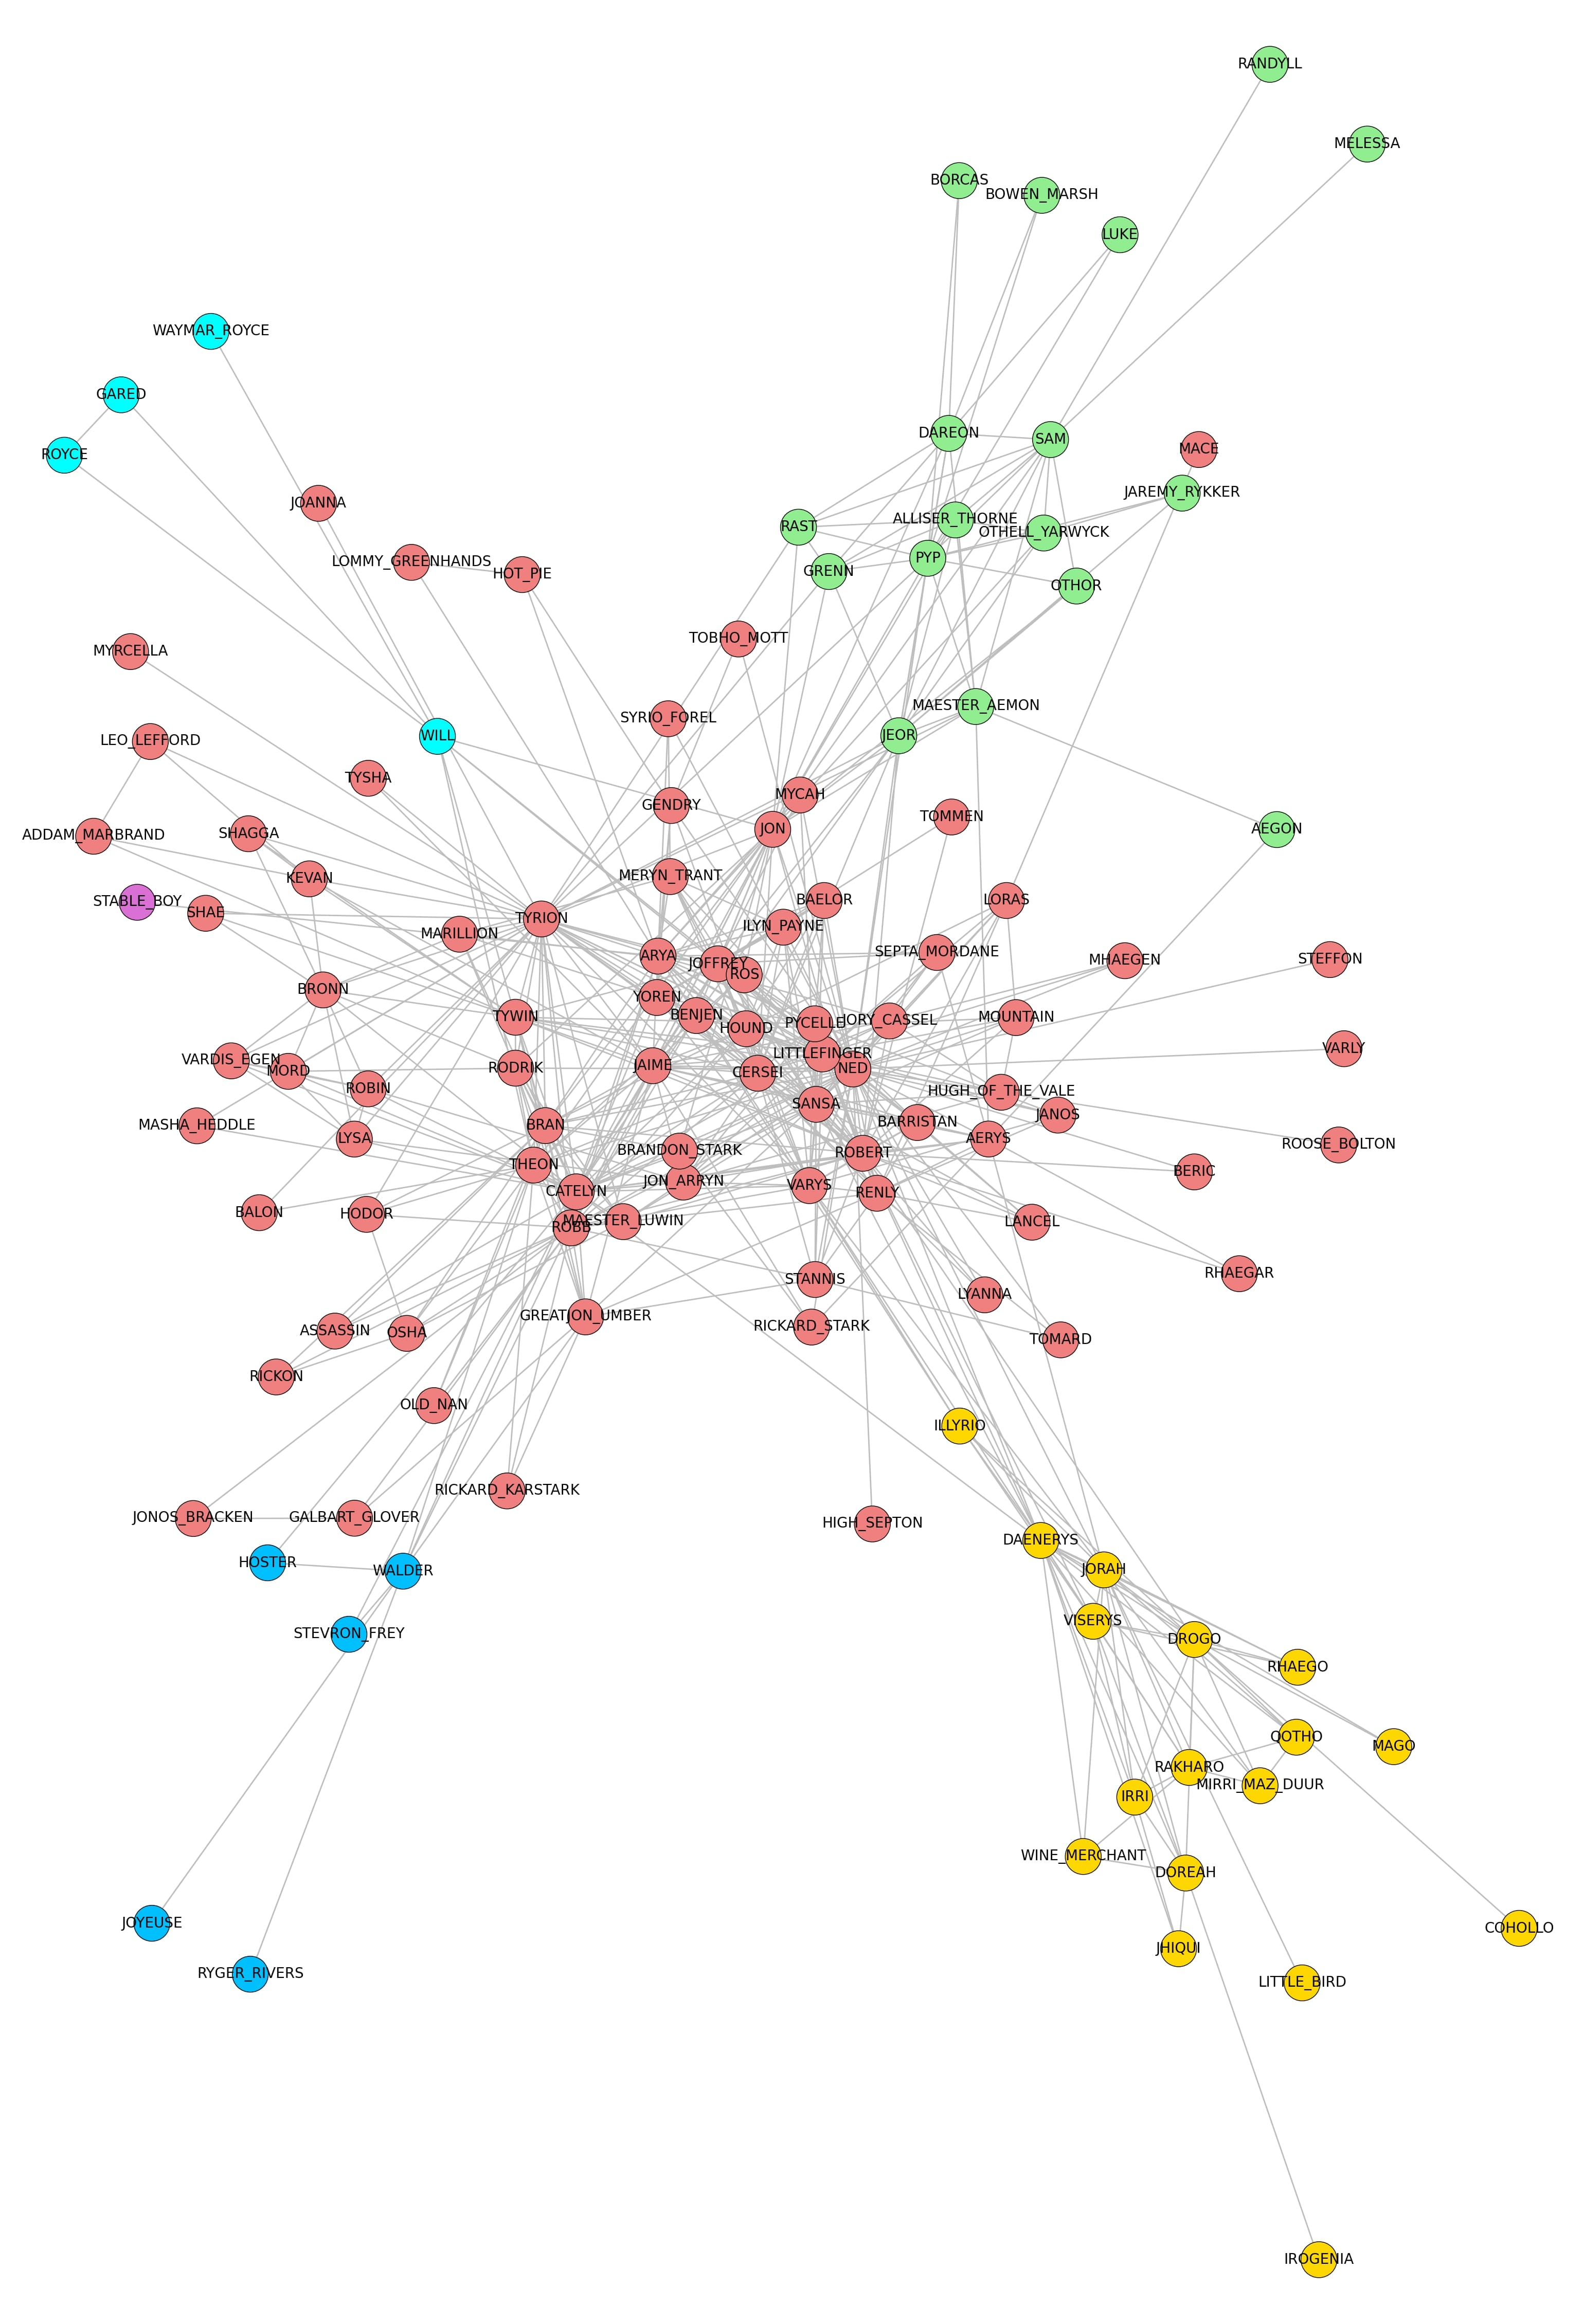
\includegraphics[width=0.4\textwidth]{img/s1/communties_g-n.jpg}
    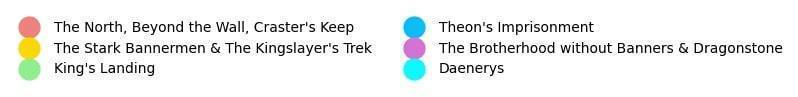
\includegraphics[width=0.35\textwidth]{img/s1/g-n_legend.jpg} \\
    \vspace{0.2cm}
    \label{fig:gn_s1}
    \caption{\small{Community detection using Girvan-Newman}}
\end{figure}

\paragraph{Louvain}

Louvain works very well in our case, reaching a 0.45 modularity score. It is able to identify 6 communities, which are essentially the same as the ones Infomap detected (King's Landing, Tyrion vs Catelyn, The Starks, The Night's Watch, The Dothraki), but with some interesting details:

\begin{itemize}
    \item \textbf{Ancestral Figures} (Aegon, Aerys, Brandon Stark): highlighted in purple, it is particularly interesting how Louvain is able to accurately select ancestral characters, which are mentioned in completely unrelated settings by people of different communities, but all during narrations and legends.
    \item \textbf{Minor Characters:} compared to Infomap, Louvain does not recognize the minor communities like the Freys and The Doomed Night's Watchmen, aggregating them to other clusters.
\end{itemize}

\begin{figure}[!h] 
    \centering
    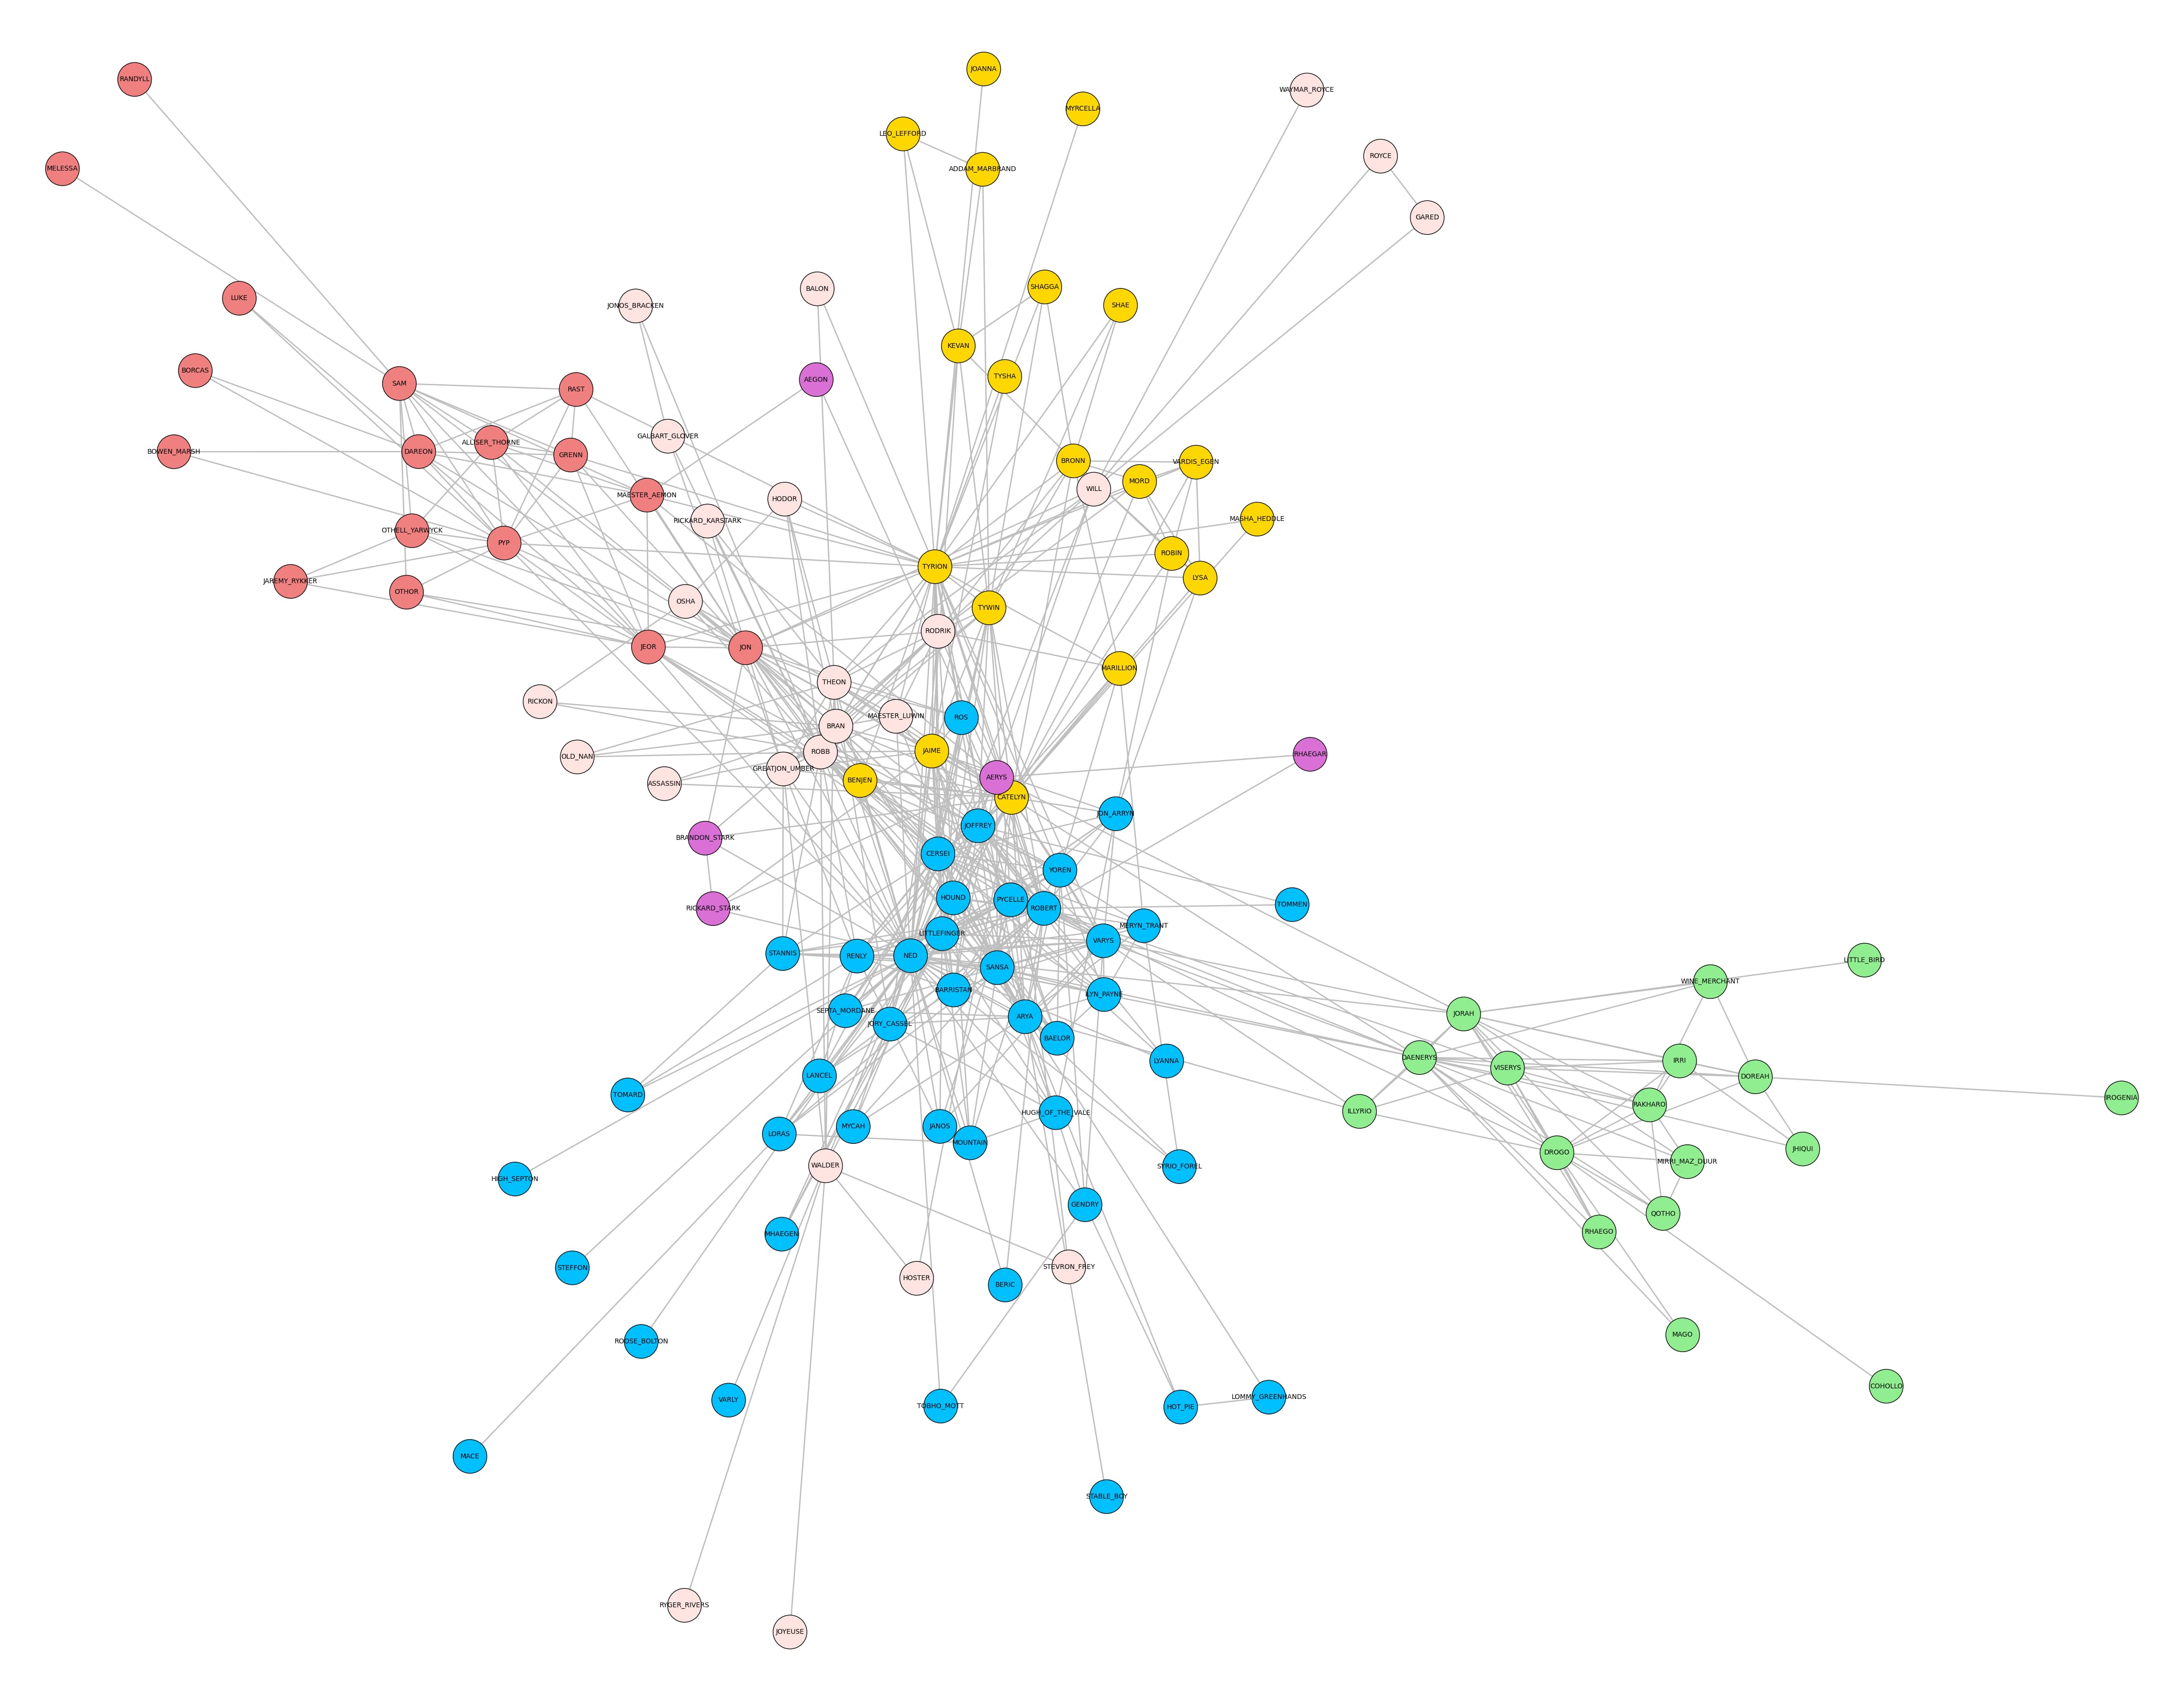
\includegraphics[width=0.35\textwidth]{img/s1/communities_louvain.jpg}
    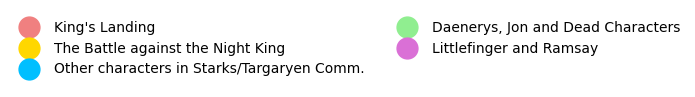
\includegraphics[width=0.3\textwidth]{img/s1/louvain_legend.jpg} \\
    \vspace{0.2cm}
    \label{fig:louvain_s1}
    \caption{\small{Community detection using Louvain}}
\end{figure}

\paragraph{Greedy Modularity Maximization (GMM)}

This approach detects 5 communities with a modularity score of 0.439.
The King's Landing community is fairly well detected, as well as the Starks, the Dothraki, the Night's Watch and the Doomed Night's Watchmen. Interestingly, although most of Jon's story line in this season is heavily related with the Night's Watch community, GMM puts it into the Stark's community. 

\begin{figure}[!h]
    \centering
    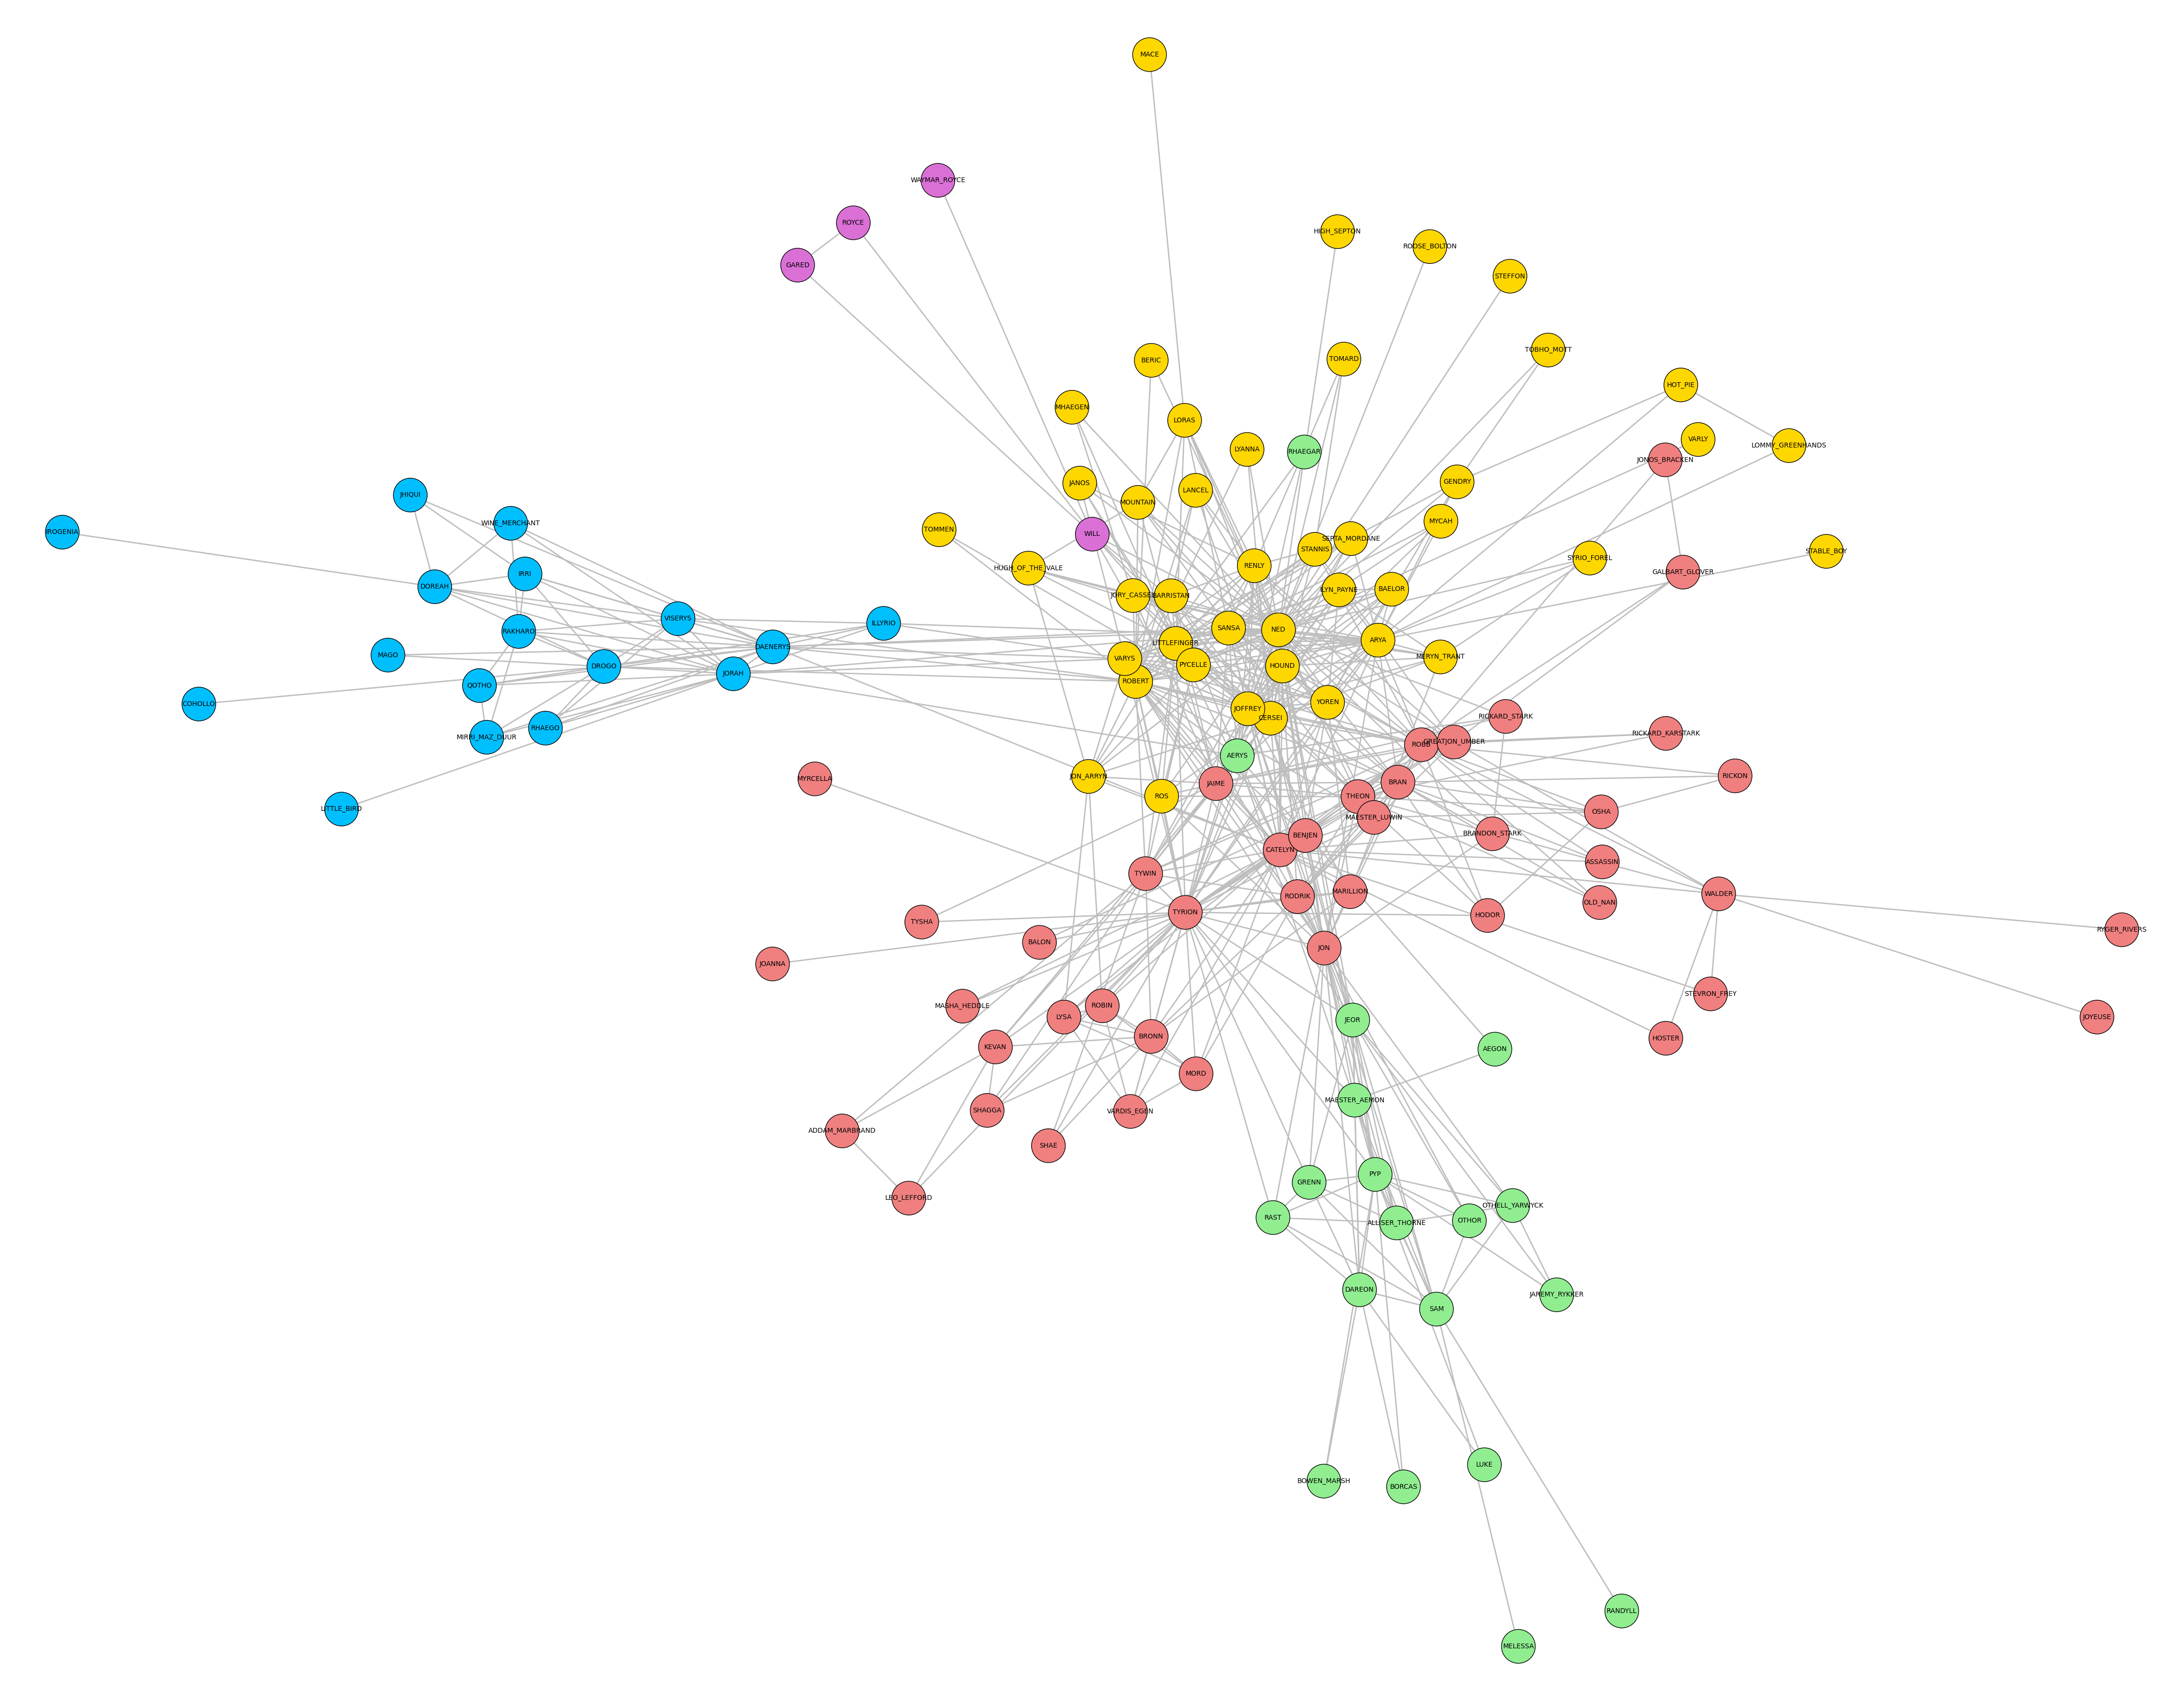
\includegraphics[width=0.35\textwidth]{img/s1/communities_gmm.jpg}
    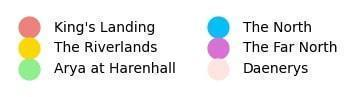
\includegraphics[width=0.35\textwidth]{img/s1/gmm_legend.jpg} \\
    \vspace{0.2cm}
    \label{fig:gmm_s1}
    \caption{\small{Community detection using GMM}}
\end{figure}


\paragraph{Spectral Clustering} detects 6 communities with a 0.39 modularity score. The communities found are the same as GMM.

\begin{figure}[!h]
    \centering
    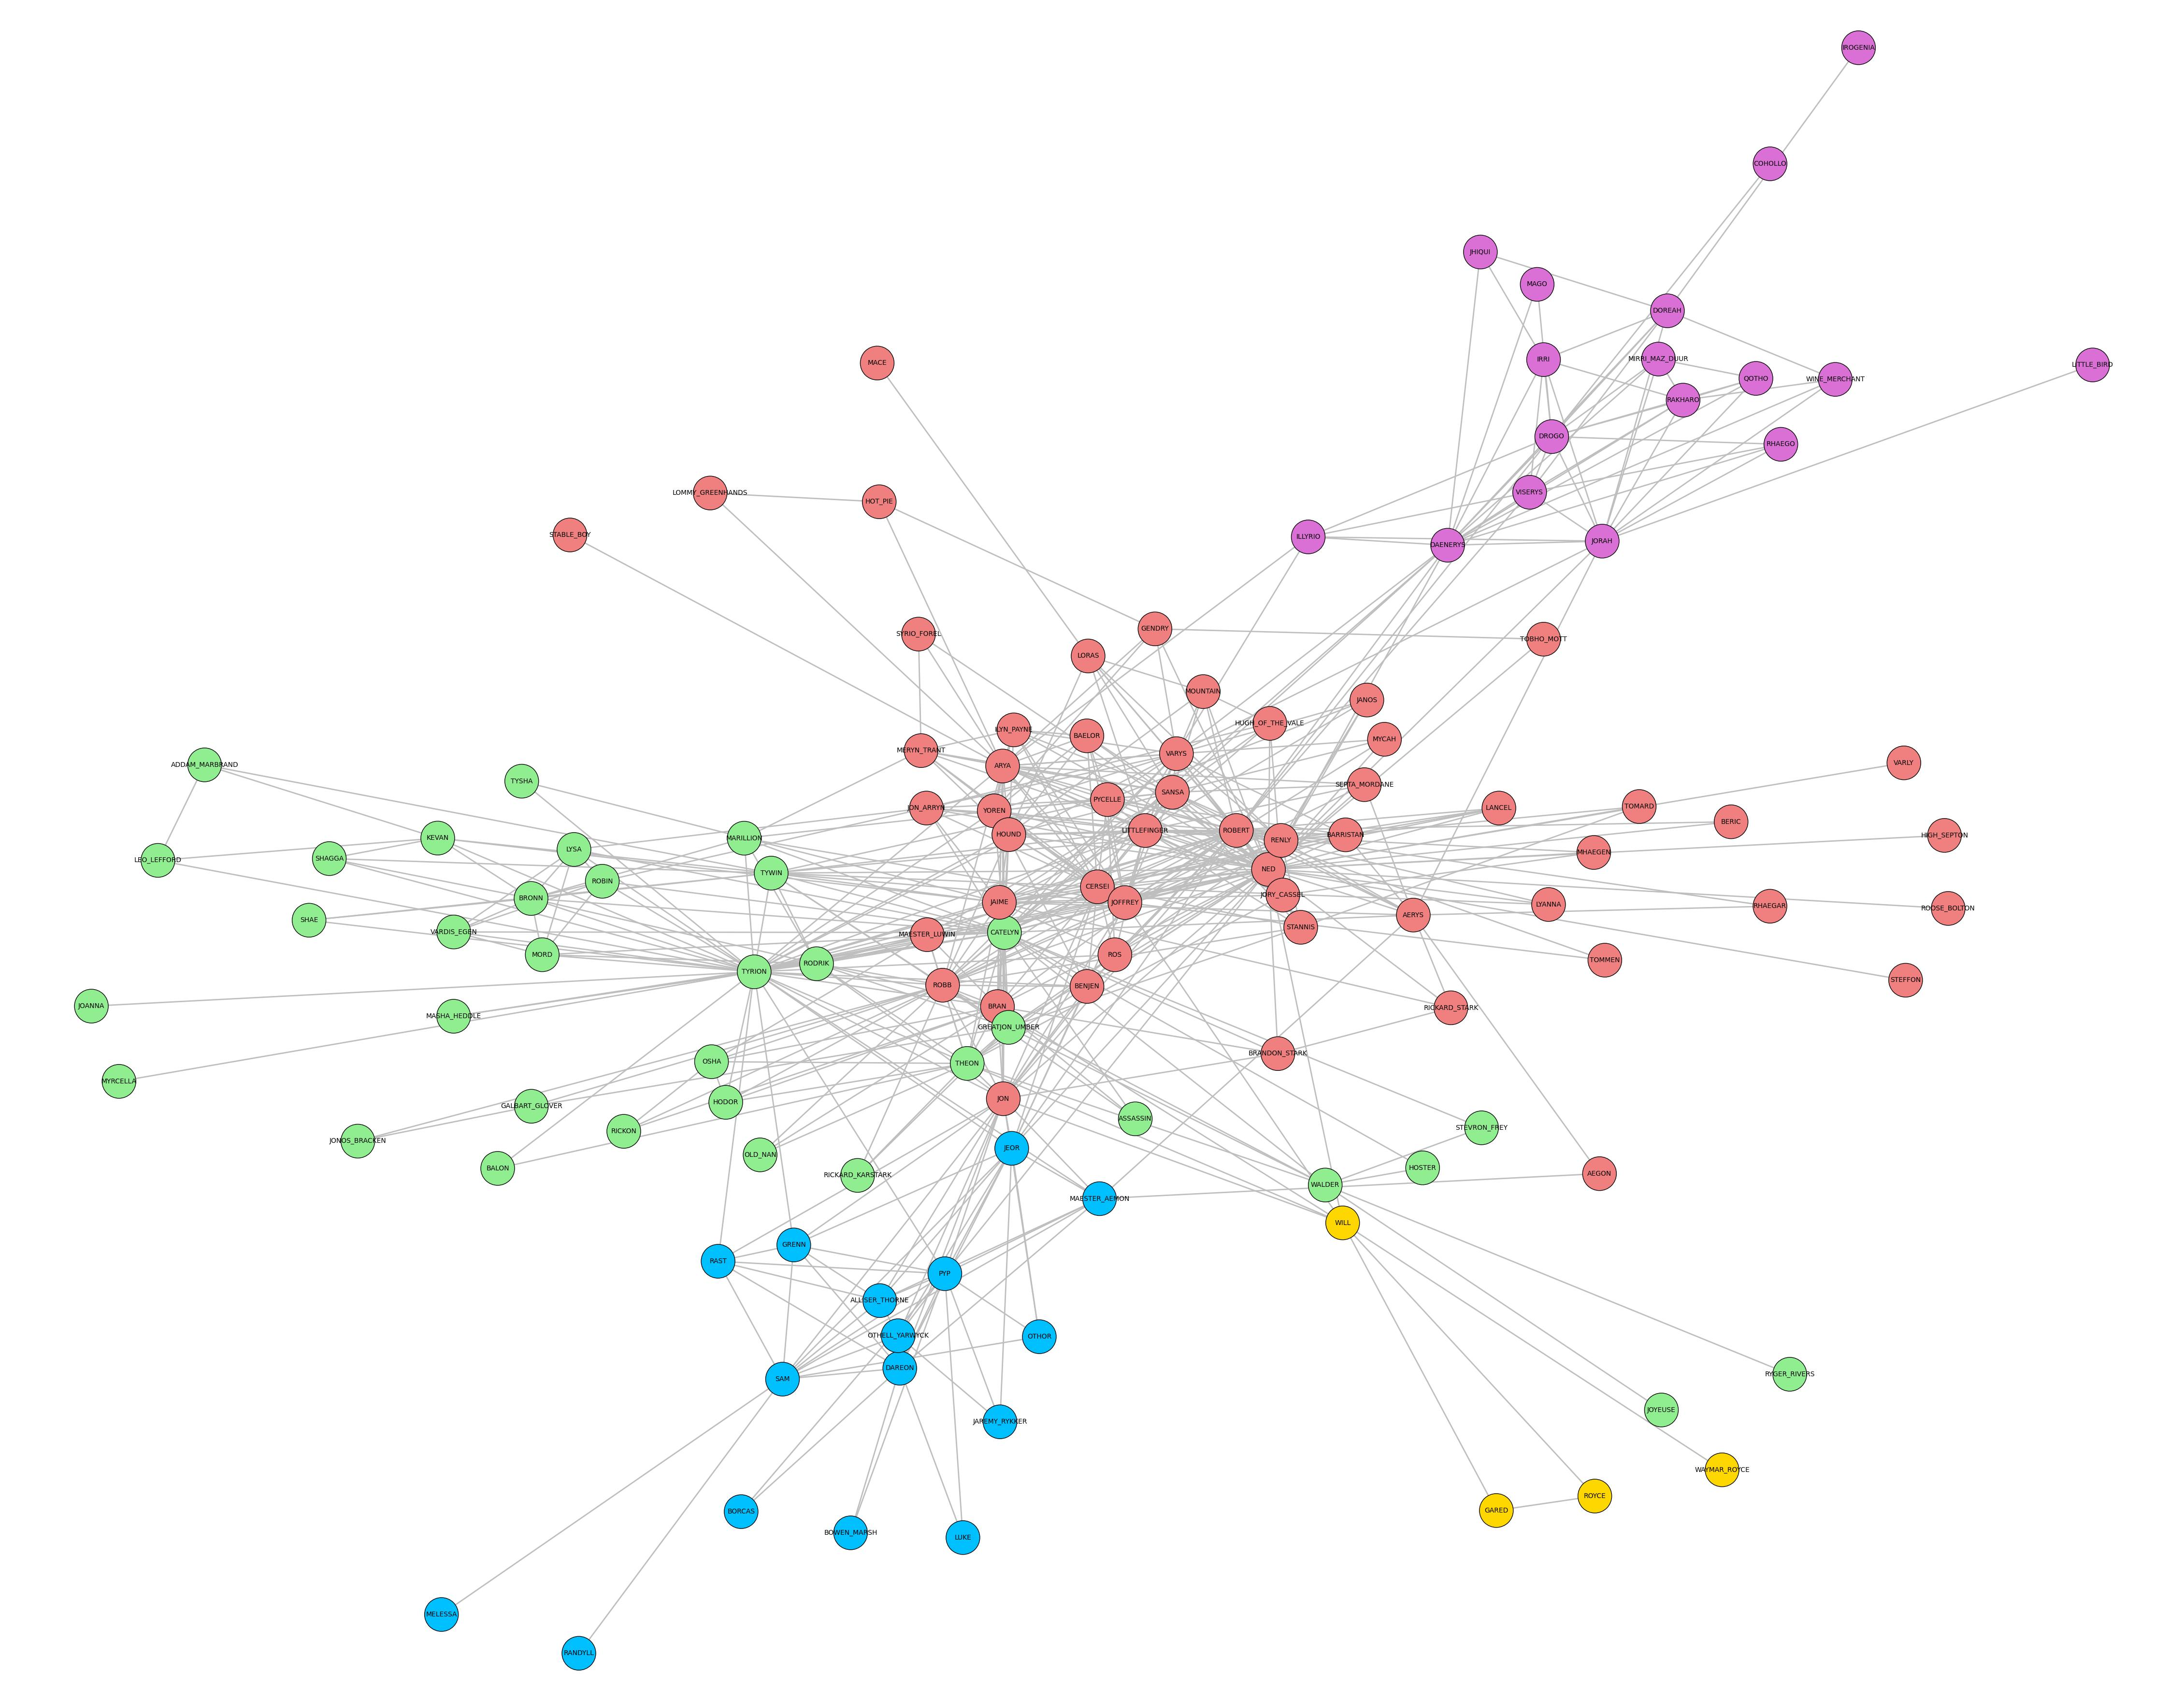
\includegraphics[width=0.4\textwidth]{img/s1/communities_sc.jpg}
    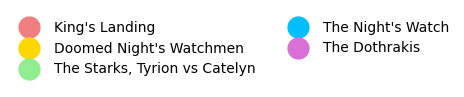
\includegraphics[width=0.35\textwidth]{img/s1/sc_legend.jpg} \\
    \vspace{0.2cm}
    \label{fig:sc_s1}
    \caption{\small{Community detection using Spectral Clustering}}
\end{figure}


\paragraph{Comparison between Methods}

Below, the plots\textsuperscript{\ref{fig:comm_comp_s1}} for number of communities per method and modularities per method are shown. 

\begin{figure}[!h]
    \centering
    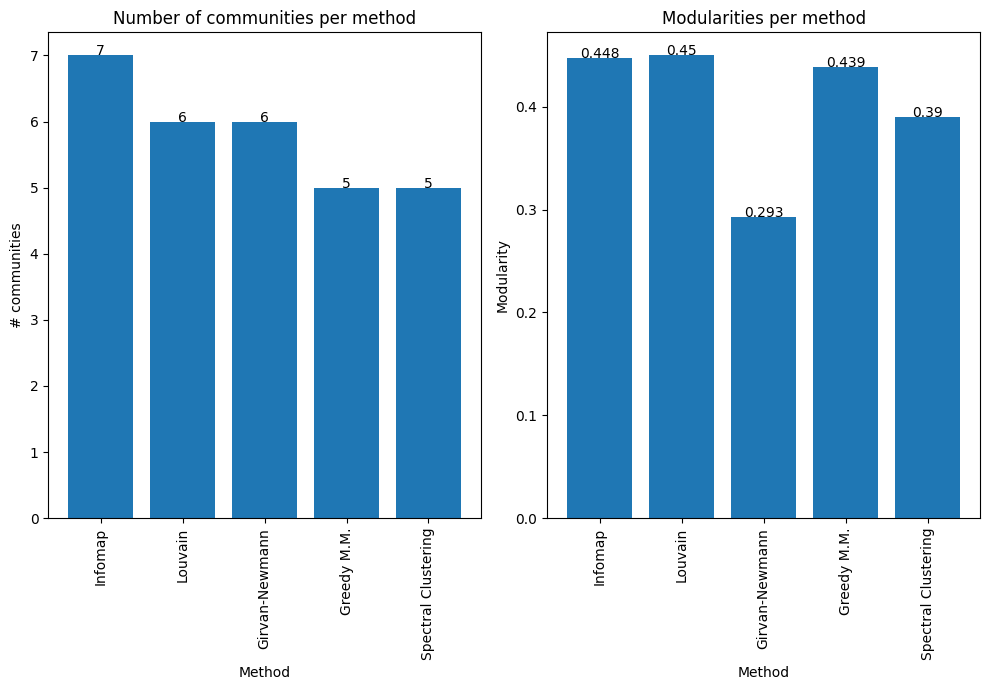
\includegraphics[width=0.48\textwidth]{img/s1/communities_comparison.jpg}\\
    \label{fig:comm_comp_s1}
    \caption{\small{Comparison between community detection methods}}
\end{figure}

Modularity-wise, all methods perform well, with the exception of Girvan-Newmann, whose modularity is substantially lower (0.275). Infomap, Louvain and Greedy Modularity Maximization present similar modularity, with Louvain having the highest. 
It is interesting to comment on the quality of the detection of the communities, especially contextualizing with information known from the actual TV series. 

Infomap\textsuperscript{\ref{fig:infomap_s1}} has detected 7 communities, which are consistent with plot lines. Among those, it detects the community of the Freys, which don't really contribute to the story much, at least right now. Louvain\textsuperscript{\ref{fig:louvain_s1}} is able to recognize 6 communities, very similarly to Infomap, while not recognizing the minor cluster of the Doomed Night's Watchmen. Though, Louvain is able to reliably extract a community of ancestral characters which are only spoke about in narrations. This is very surprising since there isn't any strong evidence of links between such nodes together. Greedy Modularity Maximization\textsuperscript{\ref{fig:gmm_s1}} detects 5 communities, which are the more prominent and important ones. The same can be said for Spectral Clustering\textsuperscript{\ref{fig:sc_s1}}.
For these reasons, the best algorithms in this context are Infomap, Louvain and, in a more simplistic way, GMM. 
The Grivan-Newmann\textsuperscript{\ref{fig:gn_s1}} algorithm detects the majority of the communities correctly; however, the Starks and King's Landing are considered as a single community, likely because of the bonds some characters have with both communities.


\subsubsection{Robustness}

\paragraph{Random Nodes Removal}

First of all, various numbers of nodes are removed at random, and basic metrics have been recomputed. The tables below show the results.

\begin{table}[!h]
    \centering
    \small
    \begin{tabular}{c|c|c|c} 
        Nodes Removed & Avg. Shortest Path & Diam. & Compon. \\
        \hline
        0 (Original) & 2.644 & 6 & 1 \\
        5	& 2.620	& 6	& 2 \\
        10	& 2.688	& 6	& 1 \\
        15	& 2.950	& 7	& 7 \\
        20	& 2.595	& 6	& 4 \\
        25	& 2.731	& 6	& 2 \\
        30	& 2.765	& 6	& 6 \\
        35	& 2.518	& 5	& 2 \\
        \hline 
    \end{tabular} \\
    \caption{Changes in Network Metrics after random nodes removal}
    \label{tab:rand_s1}
\end{table}


\begin{table}[!h]
    \centering
    \small
    \begin{tabular}{c|c|c|c|c|c} 
        \parbox{1cm}{Nodes Remov.} & \parbox{1cm}{Avg. Between.} & \parbox{1cm}{Avg. Closeness} & \parbox{1cm}{Avg. Eigenvector} & \parbox{1cm}{Avg. Harmonic} & \parbox{1cm}{Avg. Degree} \\
        \hline
        0 (Orig.)  & 0.013 & 0.389 & 0.059 & 0.018 & 0.069 \\
        5  & 0.013 & 0.386 & 0.060 & 0.386 & 0.060 \\
        10 & 0.014 & 0.383 & 0.061 & 0.383 & 0.061 \\
        15 & 0.016 & 0.314 & 0.061 & 0.314 & 0.061 \\
        20 & 0.014 & 0.375 & 0.064 & 0.375 & 0.064 \\
        25 & 0.017 & 0.371 & 0.067 & 0.371 & 0.067 \\
        30 & 0.016 & 0.337 & 0.063 & 0.337 & 0.063 \\
        35 & 0.016 & 0.399 & 0.071 & 0.399 & 0.071 \\
        \hline 
    \end{tabular}
    \caption{Changes in network centrality after random nodes removal}
    \label{tab:rand_cent_s1}
\end{table}

From the tables\textsuperscript{\ref{tab:rand_s1},\ref{tab:rand_cent_s1}}, it is evident that metrics change. The average shortest path increases as more nodes are removed, although by not a huge margin. Still, this suggests some loss of robustness. The diameter fluctuates but stays around 6, as in the original network. The number of components drastically changes with node removal, especially in the case of the removal of 15 nodes, showing that the network is vulnerable to fragmentation.

Average betweenness centrality increases slightly after node removal, showing that nodes may become more critical in their role of connecting other nodes. Average closeness centrality decreases, which is especially visible when 15 nodes are removed. 
Average eigenvector centrality increase slightly. Central nodes in terms of influence become slightly more pronounced.
Average harmonic centrality increases drastically from 0.018 to around 0.38. Degree centrality fluctuates, indicating that while the total number of connections decreases with node removal, remaining nodes tend to become more central.

Overall, the removal of random nodes, without having any other insight on how to attack the network, shows that the network is not highly robust, as evidenced by its growing fragmentation. Some characters also remain completely isolated, especially when 20 nodes are removed. Though, it is worth considering that we are targeting a lot of nodes, without having a relatively great impact on the network.


\paragraph{Centrality-based Node Removal}

To assess better the robustness of the network, it is possible to attack it by removing the most central nodes, according to betweenness centrality. Characters with high betweenness centrality often serve as bridges or intermediaries between different parts of the network. Removing these characters can fragment the network significantly.

\begin{table}[!h]
    \centering
    \small
    \begin{tabular}{c|c|c|c} 
        Nodes Removed & Avg. Shortest Path & Diam. & Compon. \\
        \hline
        0 (Original) & 2.644 & 6 & 1 \\
        1   & 2.772 & 6 & 5 \\
        3	& 2.982 & 6 & 8 \\
        5	& 3.156 & 6 & 9 \\
        \hline 
    \end{tabular} \\
    \caption{Changes in Network Metrics after centrality-based nodes removal}
    \label{tab:my_label}
\end{table}


\begin{table}[!h]
    \centering
    \small
    \begin{tabular}{c|c|c|c|c|c} 
        \parbox{1cm}{Nodes Remov.} & \parbox{1cm}{Avg. Between.} & \parbox{1cm}{Avg. Closeness} & \parbox{1cm}{Avg. Eigenvector} & \parbox{1cm}{Avg. Harmonic} & \parbox{1cm}{Avg. Degree} \\
        \hline
        0 (Orig.)  & 0.013 & 0.389 & 0.059 & 0.018 & 0.069 \\
        1	& 0.013 & 0.348 & 0.058 & 0.348 & 0.058 \\
        3	& 0.014 & 0.307 & 0.055 & 0.307 & 0.055 \\
        5	& 0.015 & 0.285 & 0.054 & 0.285 & 0.054 \\
        \hline 
    \end{tabular}
    \caption{Changes in network centrality after centrality-based nodes removal}
    \label{tab:my_label}
\end{table}

With the removal of just a few, but central, nodes, the network shows a massive fragmentation in components. The average shortest path increases, but the network diameter stays stable at 6. 

Betweenness centrality increases, which is expected, as the remaining nodes take on more intermediary roles. Closeness centrality decreases, showing that the remaining nodes are on average, further from each other. Eigenvector centrality decreases, suggesting that the influence of remaining nodes is lessened. Harmonic centrality massively increases due to the removal of key nodes affecting network distances.
Degree centrality decreases, indicating that the remaining nodes are less connected.

Overall, we can see that this method is more effective at testing the robustness of the network, that in this case reveals itself to be not robust to targeted attacks of node removal. This makes sense since important characters, especially those who serve as bridges between different parts of the network, play crucial roles in maintaining network cohesion.




\subsubsection{Link Prediction between Existing Nodes}

\paragraph{Preferential Attachment}
In the tables below are illustrated the results given by the Preferential Attachment method. More specifically are reported the top five connections between two nodes that are the ones with the highest score.
\begin{table}[!h]
    \centering
    \small
    \begin{tabular}{c|c|c} 
    First node & Second node & Score \\
    \hline
    Sansa & Tyrion & 1066 \\
    Littlefinger & Robb	& 780 \\
    Ned & Drogo & 741 \\
    Tyrion & Daenerys &	738 \\
    Renly & Tyrion & 697 \\
    \hline 
    \end{tabular}
    \caption{Preferential attachement: Top 5 connections with highest scores}
    \label{tab:my_label}
\end{table}

Link predictions make sense for the most part. Sansa and Tyrion don't interact in season one, but in the following seasons, they become very close, as although they forcefully get married, they develop a strong friendship and alliance. Tyrion does not interact with Daenerys in season 1. Nonetheless, their link prediction is surprisingly strong, and indeed in the later seasons he will become Daenery's advison and hand of the queen. Littlefinger betrayed Ned, who is Robb's father, and this led to Ned's death; Robb is filled with rage and wants to declare war, which would make him and Littlefinger interact.
Ned and Drogo would have probably met if the two had not died and Viserys' plan to claim the Iron Throne through the help of the Dothraki had gone through.
Instead, Renly and Tyrion follow different plot lines, although Renly is interested in claiming the Iron Throne too. 


\subsubsection{Link Prediction between New Nodes}

\paragraph{Adding One Node with One Edge}

The Barabasi-Albert Model is exploited to add one single node with a single edge. This method connects the node to Arya Stark with a preferential attachment score of 29, which is realatively low. The prediction is realistic given Arya's adventurous and mobile nature, interacting with lots of minor characters.

\paragraph{Adding One Node with 10 Edges}

The results are displayed below.

\begin{table}[!h]
    \centering
    \small
    \begin{tabular}{c|c} 
    Node & Score \\
    \hline
    Ned	& 580 \\
    Robert	& 370\\
    Catelyn	& 370\\
    Arya & 290\\
    Littlefinger &  270\\
    Varys & 220\\
    Tywin  &180\\
    Pycelle & 170\\
    Maester Luwin & 110\\
    Vardis Egen &	70\\
    \hline 
    \end{tabular} 
    \vspace{0.2cm}
    \caption{Link prediction}
    \label{tab:my_label}
\end{table}

The results show that central characters, such as Ned, tend to link to characters with a higher connectivity, which is supported by the high scores. Arya does also interact with major characters, such as with Ned and Tywin. A similar observation can be made for Pycelle and Maester Luwin: they are not central characters, but being both maesters for the Stark's and Lannister's families, interact with characters with many edges.

\paragraph{Adding 10 Nodes with $x$ Edges}
Ten nodes with $x$ edges, where $x$ is the average number of edges per node, have been added. The results are displayed in the chart below.

\begin{figure}[!h]
    \centering
    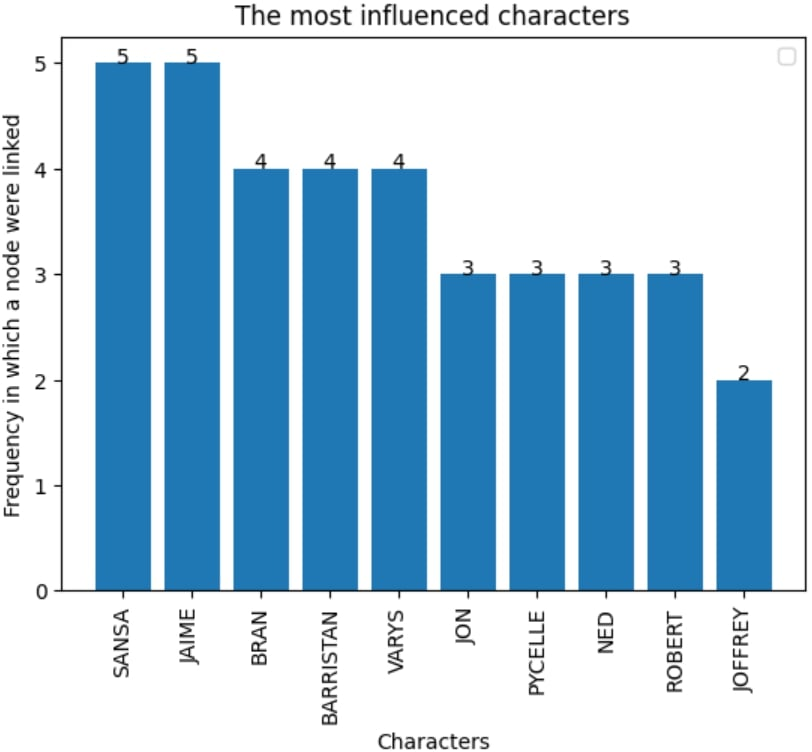
\includegraphics[width=0.4\textwidth]{img/s1/link_pred_chart.jpg}
    \vspace{0.2cm}\\
    \caption{\small{Top 10 most influenced characters by addition of 10 nodes.}}
\end{figure}


\subsection{Season 2}

\begin{figure}[!h]
    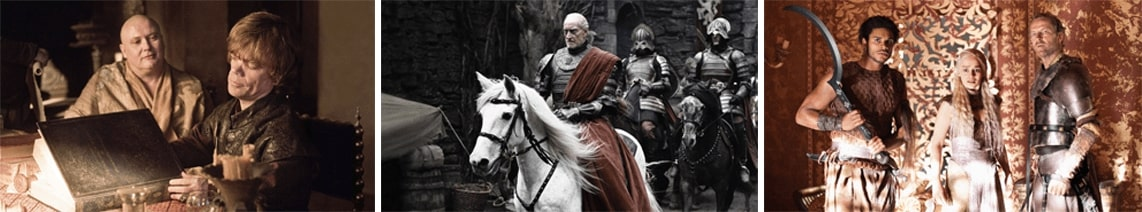
\includegraphics[width=0.48\textwidth]{img/s2/frames_s2.jpg}
\end{figure}

In order to avoid being repetitive, the analysis of the seasons following the first will focus only on selected aspects of particular relevance, and will aggregate other main relevant data in a concise table.

\begin{center}
    \vspace{5cm}
\end{center}

\begin{table}[!h]
    \centering
    \small
    \begin{tabular}{c|c}
        Description & Value  \\
        \hline
        Nodes & 129 \\
        Edges & 486 \\
        Graph Density & 0.058 \\
        Connected Graph & No \\
        Number of Components & 2 \\
        Small-World Network & Yes ($\lambda=1.08$ , $\gamma=12.84$) \\
        Diameter & 6 \\
        Avg. Shortest Path & 2.84 \\
        Avg. Degree & 7.53, range [1, 36] \\
        Most Freq. Degree & 1 \\
        Number of Bridges & 23 \\
        Deg. Assortativity Coeff. & -0.086\\
        Global Clustering Coeff. & 0.415 \\
        Average Clustering Coeff. & 0.576 \\
        \hline 
    \end{tabular}
    \vspace{0.2cm}
    \caption{Summary table for Season 2's network}
    \label{tab:my_label}
\end{table} 

\begin{figure}[!h]
    \centering
    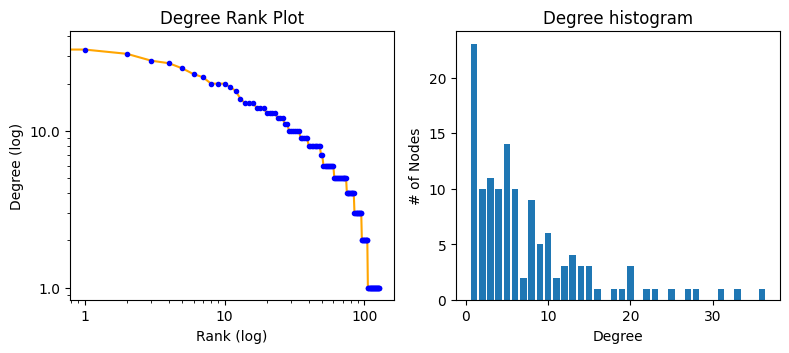
\includegraphics[width=0.5\textwidth]{img/s2/degree_plot.jpg}
    \caption{\small{Degree distribution of Season 2}}
\end{figure}

\subsubsection{Centrality}

Below we plot Season 2's interaction network where the node sizes are scaled according to PageRank centrality, and the layout is computed using the Fruchterman-Reingold force-directed layout algorithm.

\begin{figure}[!h]
    \centering
    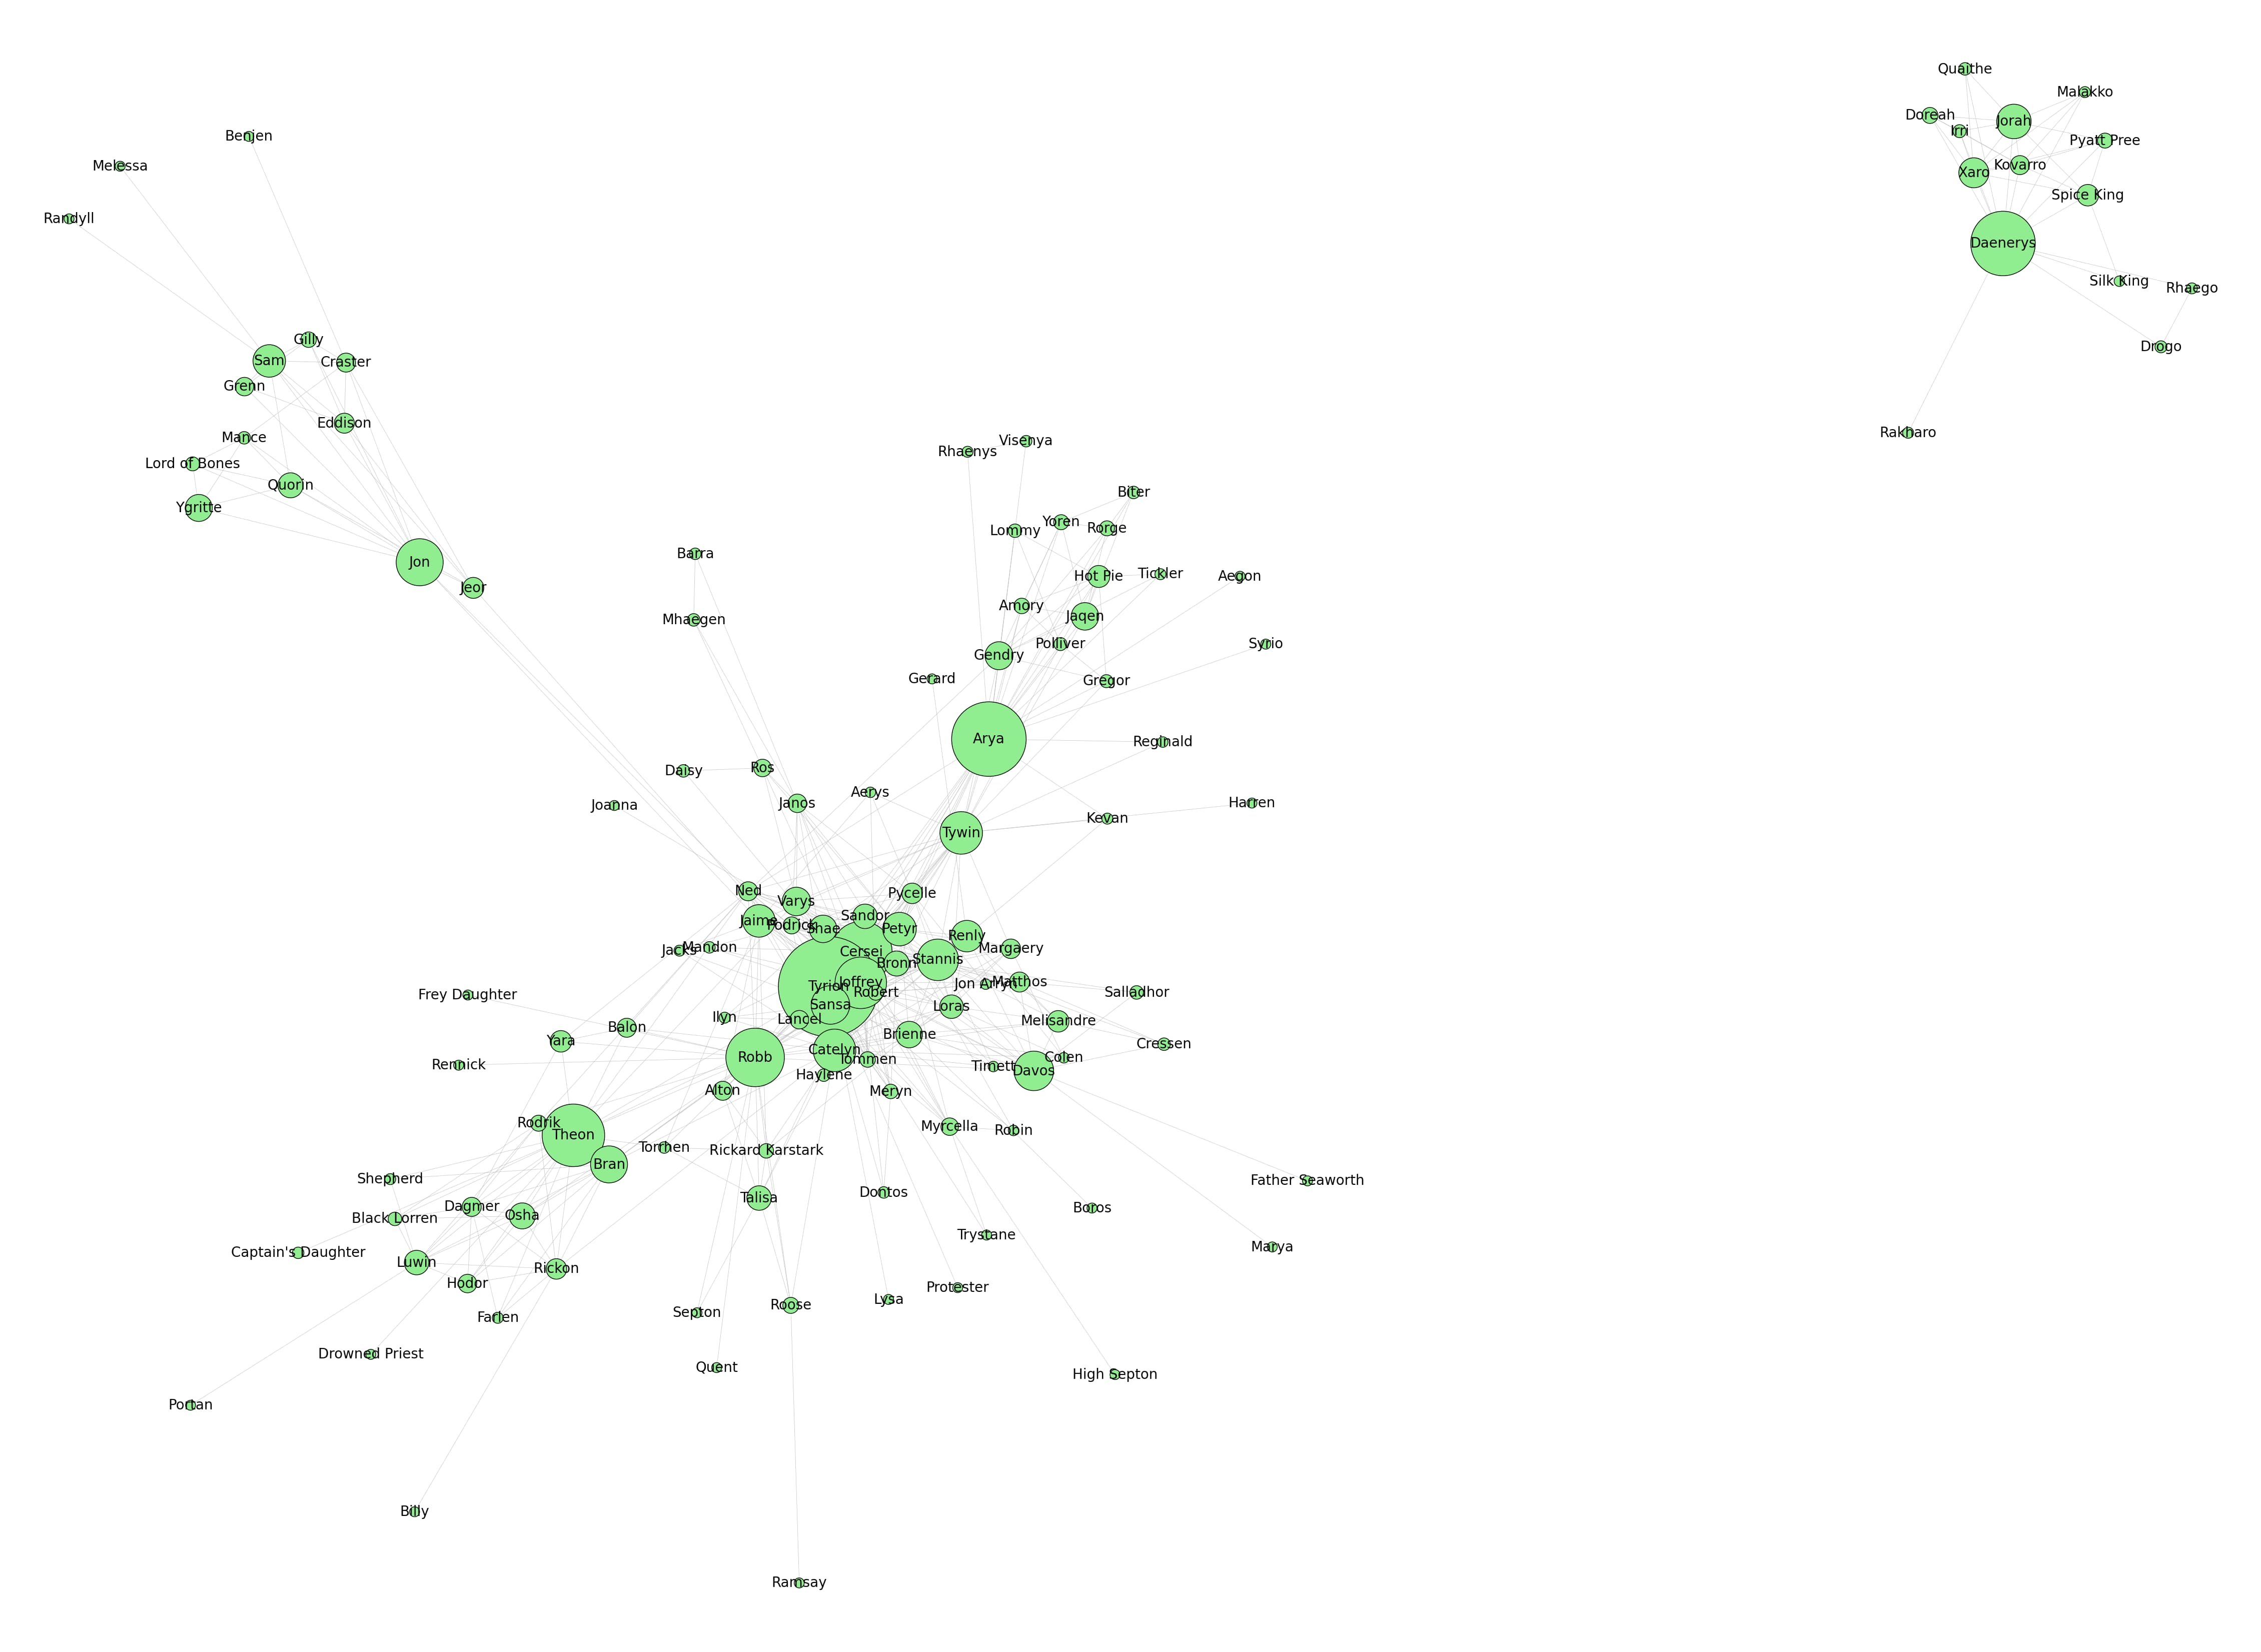
\includegraphics[width=0.37\textwidth]{img/s2/pagerank_network.jpg}
    \caption{\small{Game of Thrones, Season 2}}
\end{figure}

\begin{table}[!h]
    \centering
    \small
    \begin{tabular}{c|c|c}
        Measure & Character & \small{Highest Centrality Score} \\
        \hline
                    & Arya & 0.151 \\
                    & Tyrion & 0.141 \\
        Betweenness & Robb & 0.117 \\
                    & Jon & 0.111 \\
                    & Ned & 0.104 \\
        \hline 
                    & Tyrion & 0.477 \\
                    & Joffrey & 0.477 \\
        Closeness   & Ned & 0.462 \\
                    & Robb & 0.451 \\
                    & Cersei & 0.447 \\
        \hline 
                    & Joffrey & 0.313 \\
                    & Cersei & 0.283 \\
        Eigenvector & Tyrion & 0.277 \\
                    & Stannis & 0.222 \\
                    & Tywin & 0.216 \\
        \hline 
                    & Joffrey & 0.014 \\
                    & Tyrion & 0.014 \\
        Harmonic    & Cersei & 0.015 \\
                    & Robb & 0.015 \\
                    & Arya & 0.015 \\
        \hline
                    & Joffrey & 0.281 \\
                    & Tyrion & 0.258 \\
        Degree      & Arya & 0.211 \\
                    & Robb & 0.219 \\
                    & Cersei & 0.211 \\
        \hline
                    & Tyrion & 1.000 \\
                    & Joffrey & 0.572 \\
        Weighted Degree & Arya & 0.501 \\
                    & Theon & 0.466 \\
                    & Robb & 0.219 \\
        \hline
                    & Joffrey & 0.029 \\
                    & Tyrion & 0.028 \\
        PageRank    & Arya & 0.027 \\
                    & Robb & 0.026 \\
                    & Cersei & 0.025 \\
        \hline
    \end{tabular}
    \vspace{0.2cm}
    \caption{Top characters with highest centrality scores}
    \label{tab:my_label}
\end{table}

\begin{table}[!h]
    \centering
    \small
    \begin{tabular}{c|c}
        Centrality Measure & Mean  \\
        \hline
        Betweenness & 0.013 \\
        Closeness & 0.389 \\
        Eigenvector & 0.059 \\
        Harmonic & 0.018 \\
        Degree & 0.069 \\
        Weighted Degree & 0.1 \\
        PageRank & 0.008 \\
        \hline 
    \end{tabular} \\
    \caption{Centrality means}
    \label{tab:my_label}
\end{table}

Tyrion is arguably the most central character in Season 2. As Hand of the King, he plays a crucial role in governing King's Landing, making key decisions, and interacting with a wide range of characters. offrey, as king, holds significant influence over others, which is reflected in his high Eigenvector and PageRank scores. His actions and decisions impact nearly every character in King’s Landing, justifying his high Degree Centrality and Closeness Centrality. Robb Stark’s centrality reflects his role as the King in the North and his campaign against the Lannisters. Arya's high Betweenness Centrality reflects her role in connecting different storylines, especially during her journey in Harrenhal. Cersei’s scores demonstrate her influence within King’s Landing, especially through her manipulation and control over key characters like Joffrey. Ned’s influence continues in Season 2, particularly through the Stark family’s actions and the reverberations of his death.

\subsubsection{Triangles}

In this network, 900 triangles are present. The characters with most triangles are Joffrey (176), Cersei (151), Tyrion (141), Stannis (100), Robb (92) and Tywin (89).
They all share the interest for the Iron Throne. Joffrey, Cersei, Tywin and Tyrion are of the house Lannister, whereas Stannis and Robb are not in King's Landing but very much focused on winning the Iron Throne.


Some interesting triangles have been selected and presented in the following table and graph.

\begin{table}[!h]
    \centering
    \small
    \begin{tabular}{c|c|c}
        Triangle & Strength & Strongest Edge  \\
        \hline
        \small{(Jon, Ygritte, Qhorin)} & 209 & 110 \small{(Jon, Ygritte)} \\
        \small{(Cersei, Tyrion, Joffrey)} & 306 & 177 \small{(Cersei, Tyrion)} \\
        \small{(Cersei, Tyrion, Varys)} & 291 & 177 \small{(Cersei, Tyrion)} \\
        \small{(Cersei, Joffrey, Sansa)} & 179 & 73 \small{(Cersei, Sansa)} \\
        \small{(Tyrion, Shae, Bronn)} & 184 & 95 \small{(Tyrion, Shae)} \\
        \small{(Cersei, Tyrion, Bronn)} & 266 & 177 \small{(Cersei, Tyrion)} \\
        \small{(Robb, Catelyn, Jamie)} & 82 & 82 \small{(Robb, Catelyn)} \\
        \small{(Catelyn, Brienne, Jamie)} & 54 & 54 \small{(Catelyn, Brienne)} \\
        \small{(Catelyn, Brienne, Renly)} & 115 & 54 \small{(Catelyn, Brienne)} \\
        \small{(Daenerys, Jorah, Xaro)} & 211 & 119 \small{(Daenerys, Jorah)} \\
        \small{(Arya, Jaqen, Gendry)} & 195 & 113 \small{(Arya, Jaqen)} \\
        \hline
    \end{tabular}
    \vspace{0.2cm}
    \caption{Strength of interesting triangles}
    \label{tab:my_label}
\end{table}

\begin{figure}[!h]
    \centering
    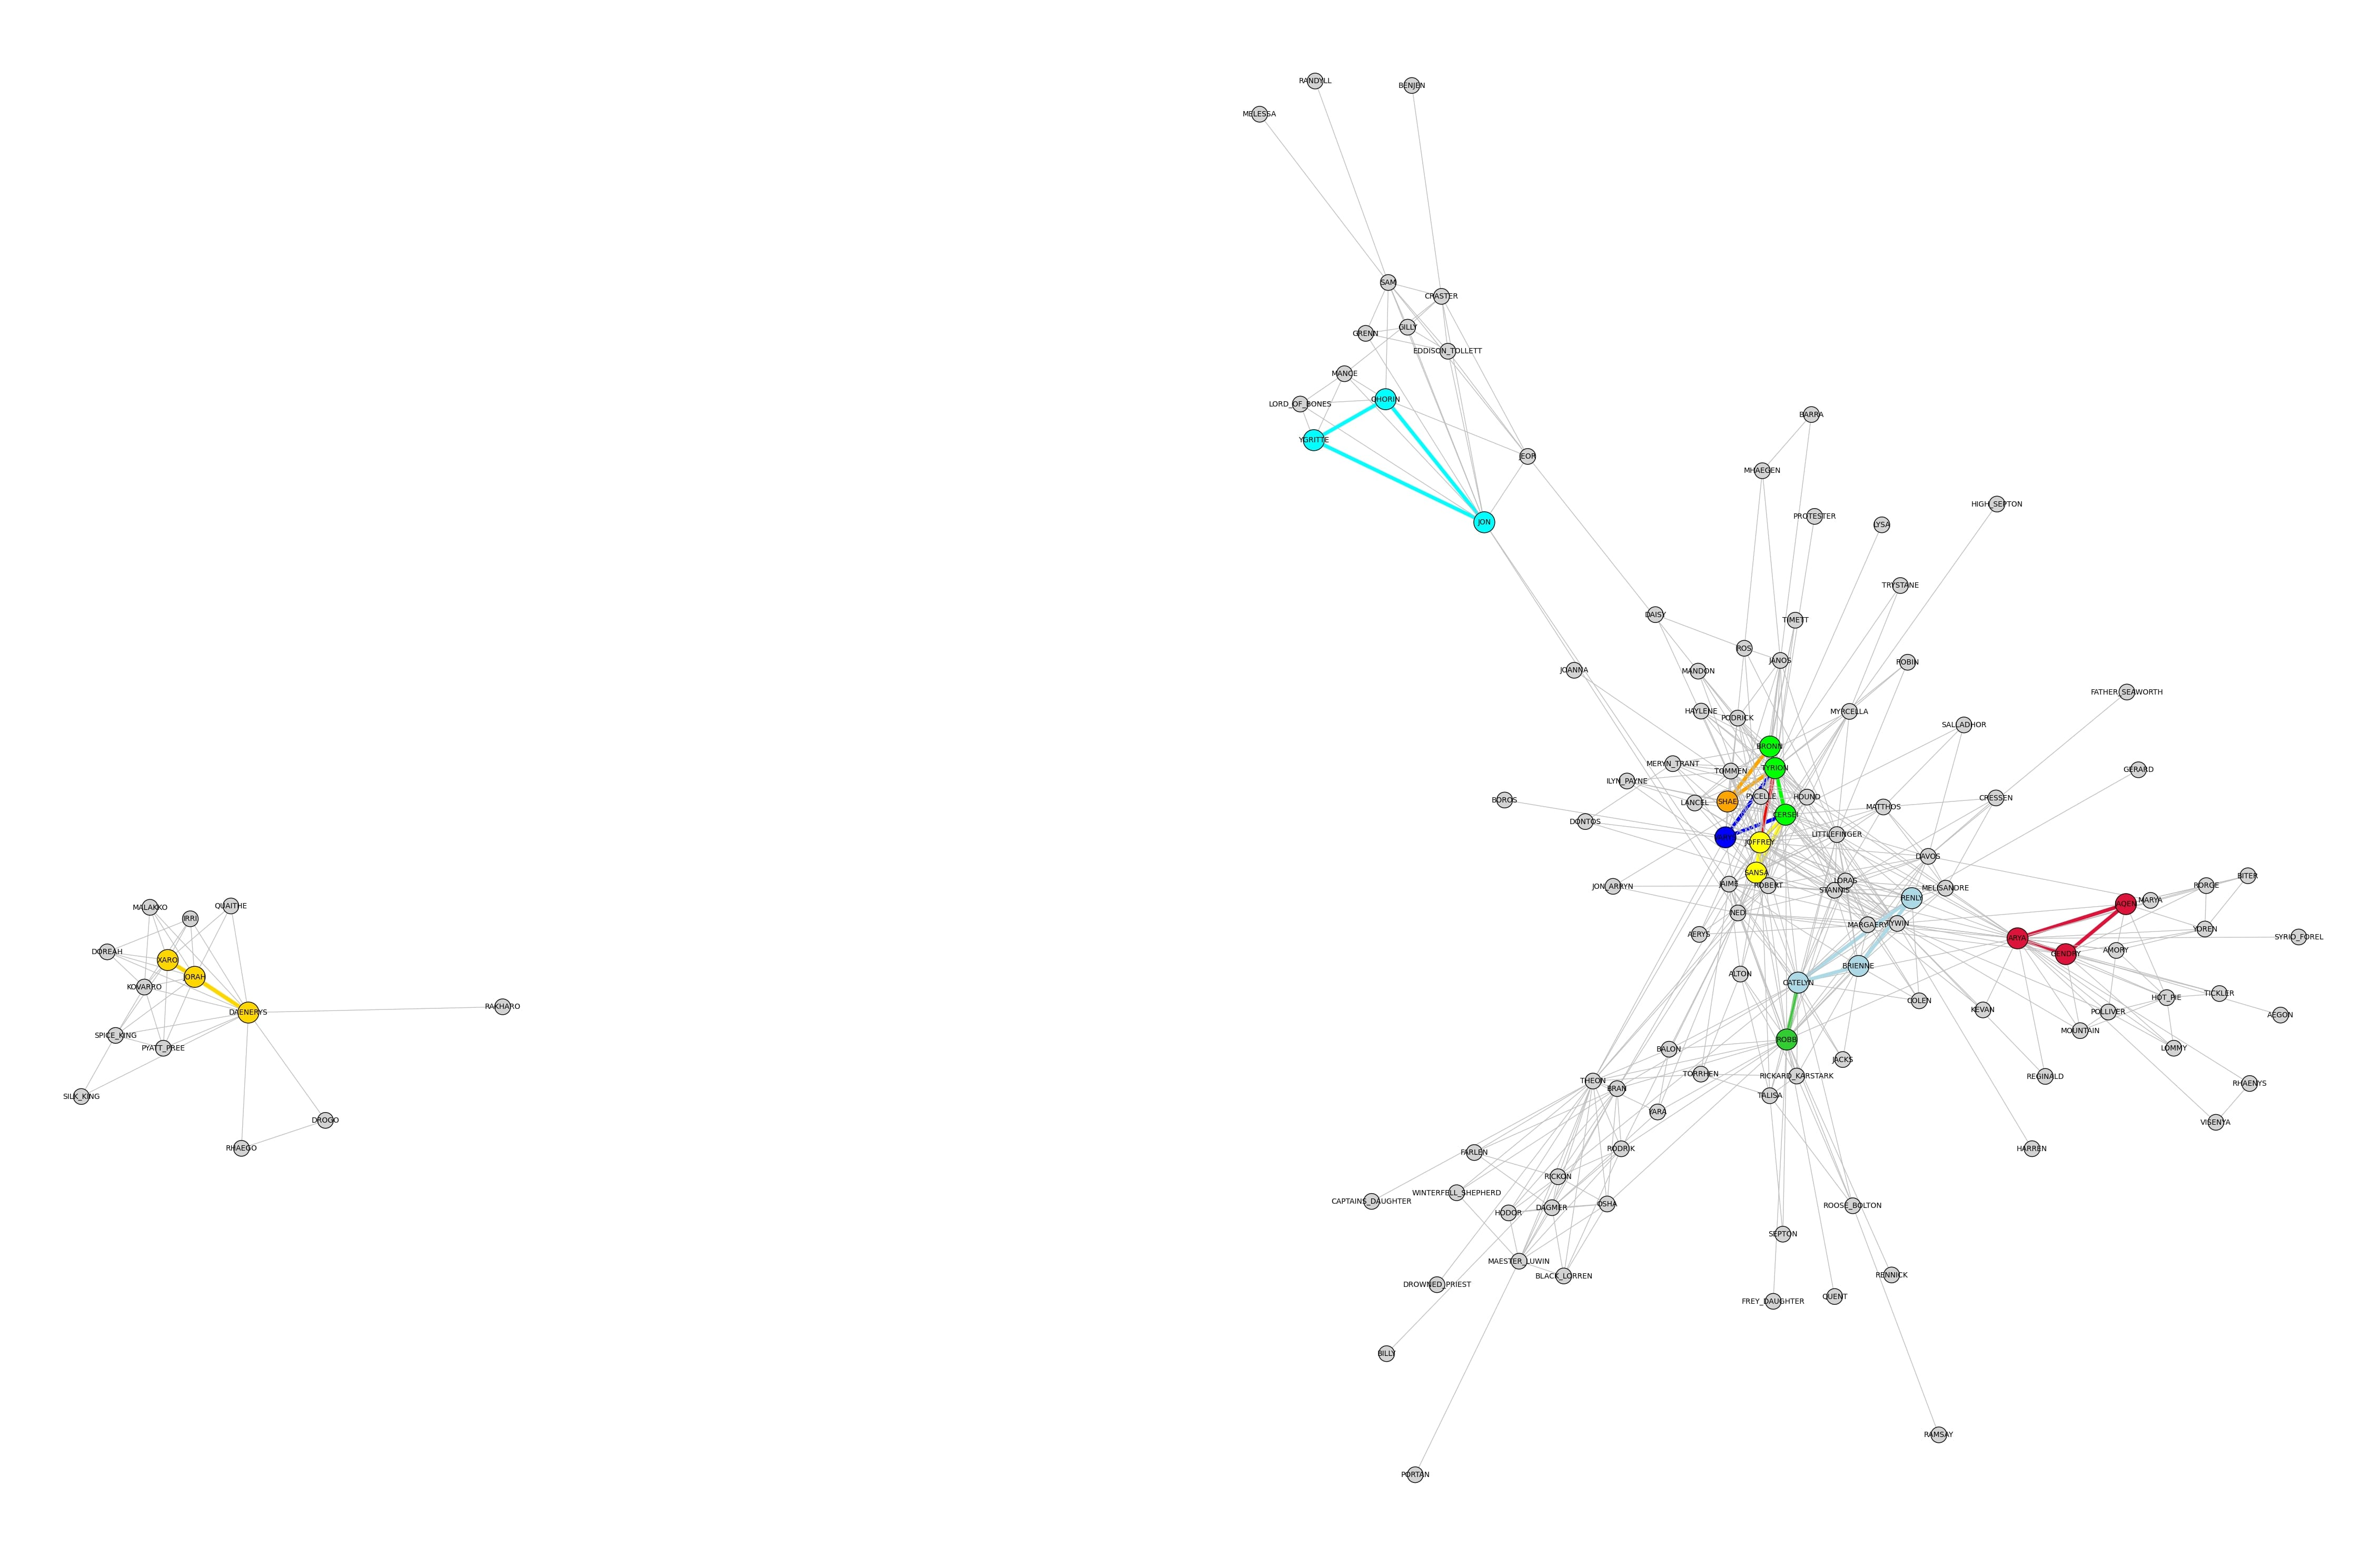
\includegraphics[width=0.5\textwidth]{img/s2/triangles.jpg}
    \caption{\small{Interesting triangles in Season 2}}
\end{figure}

\newpage

In the Far North, Jon forms a strong triangle with Ygritte and Qhorin. Qhorin's party finds a group of lookouts and ambushes them. Jon hesitates in killing one, realizing the wildling, Ygritte, is a woman. Jon and Ygritte will fall in love ($weight_{j,y}=110$). 
Cersei has strong bonds with his son, Joffrey, and with her brother Tyrion ($weight_{c,t}=177$). Cersei strongly hates Tyrion, which is evident by the strongest edge being between them when a common triangle is considered.

\begin{figure}[!h]
    \centering
    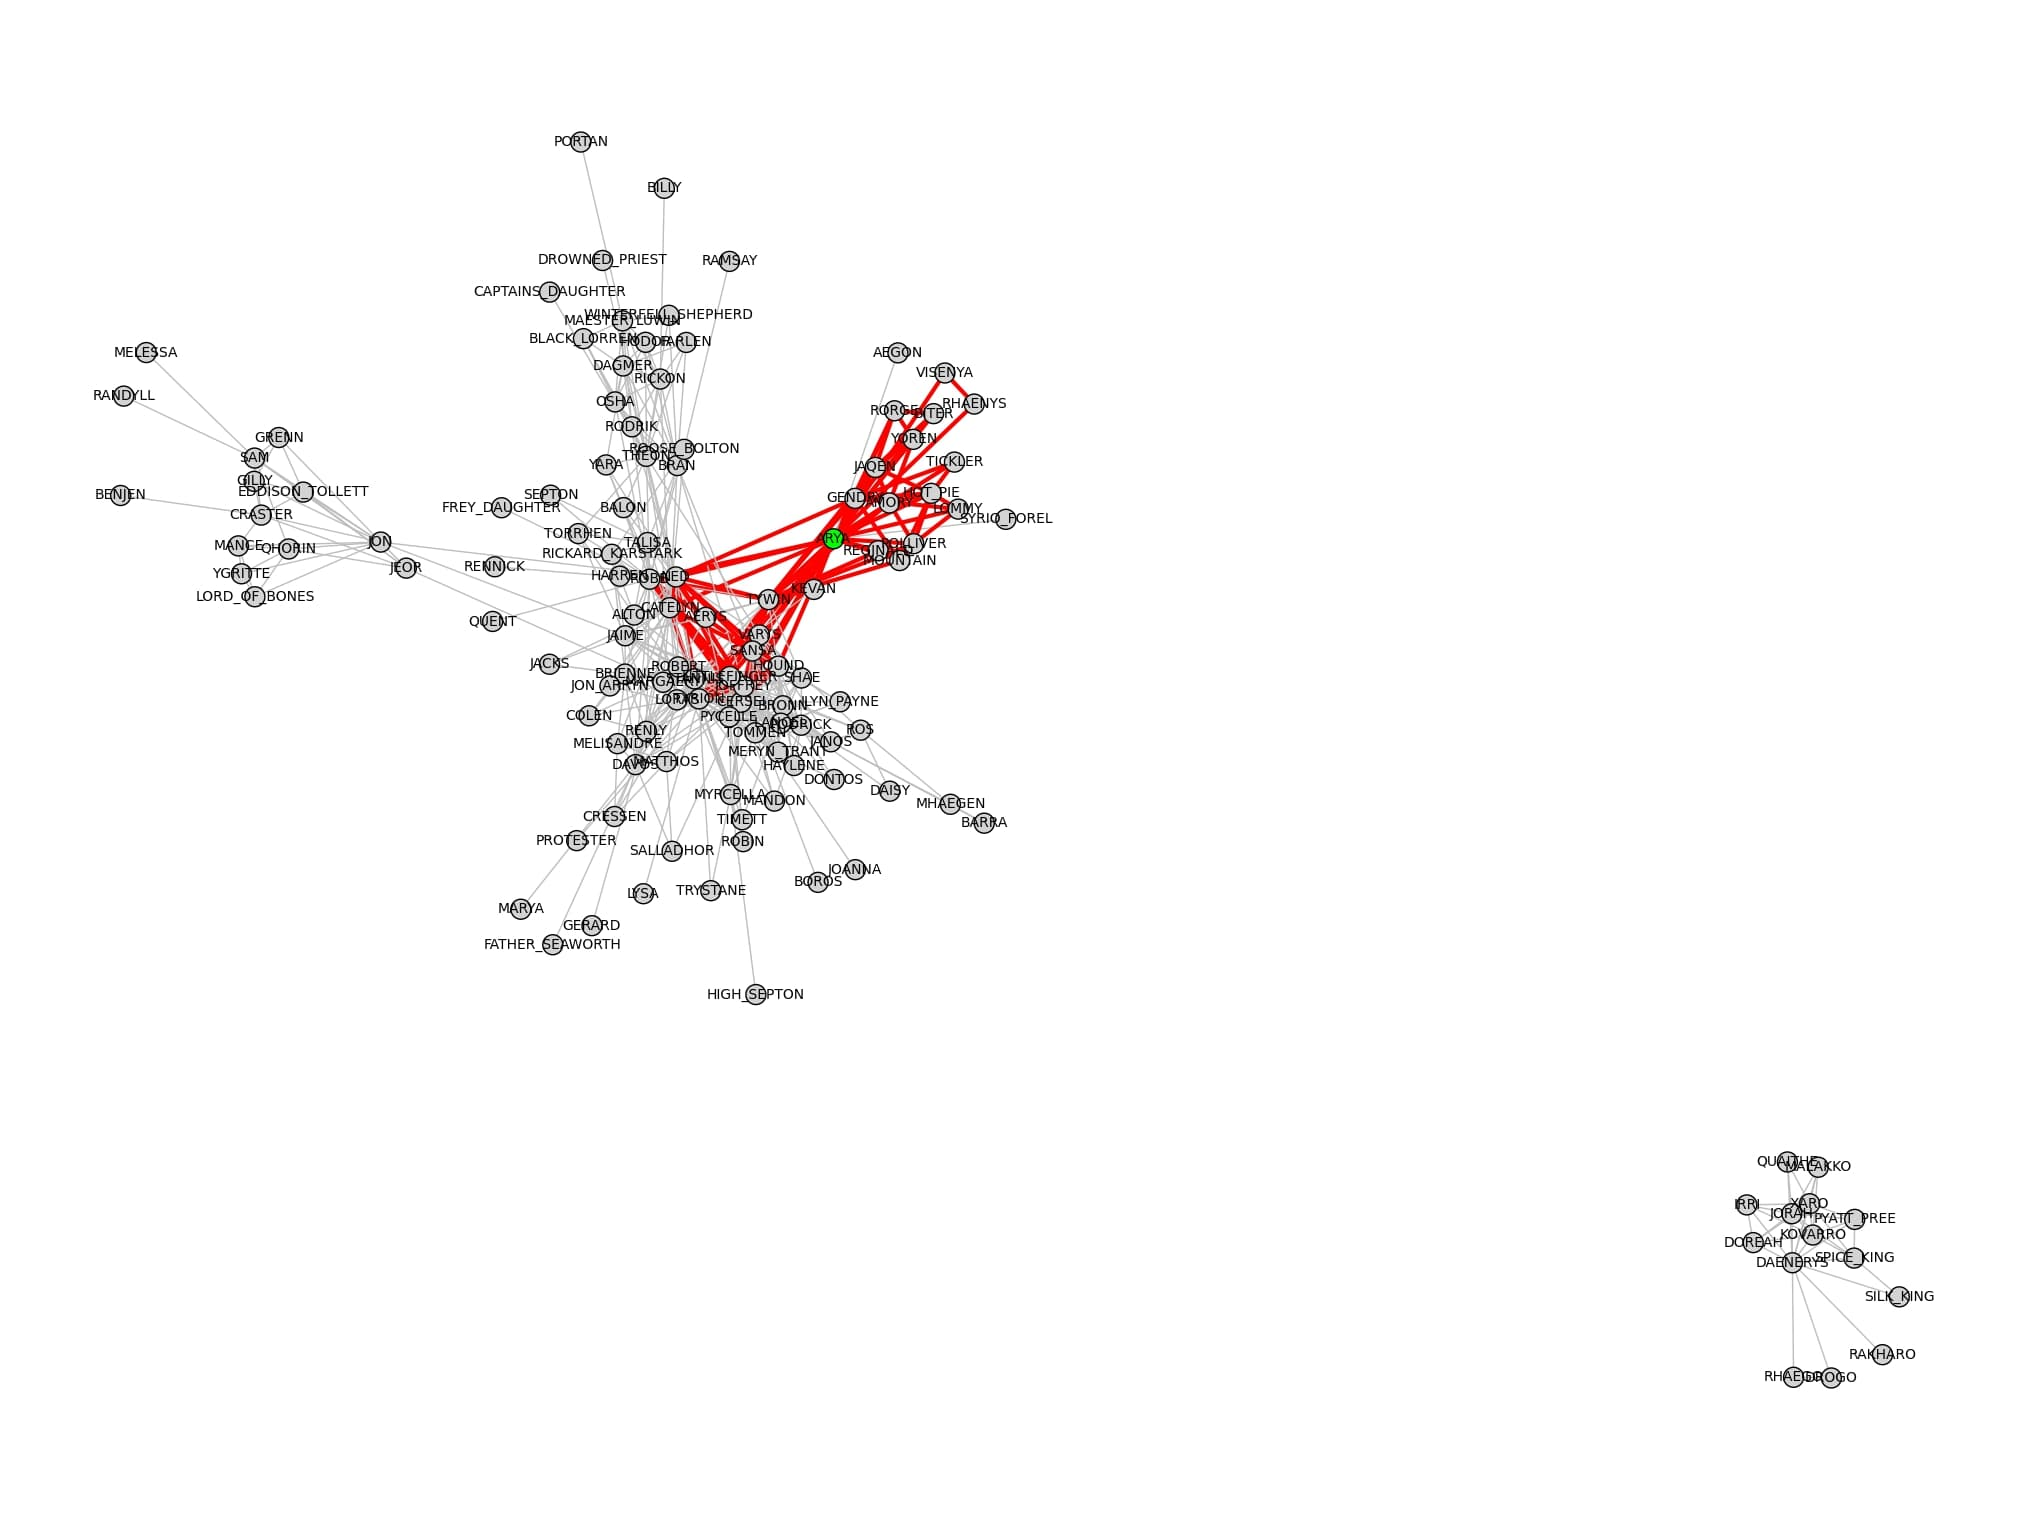
\includegraphics[width=0.37\textwidth]{img/s2/triangles_arya.jpg} \\
    \caption{\small{All triangles involving Arya Stark in Season 2}}
\end{figure}

\begin{figure}[!h]
    \centering
    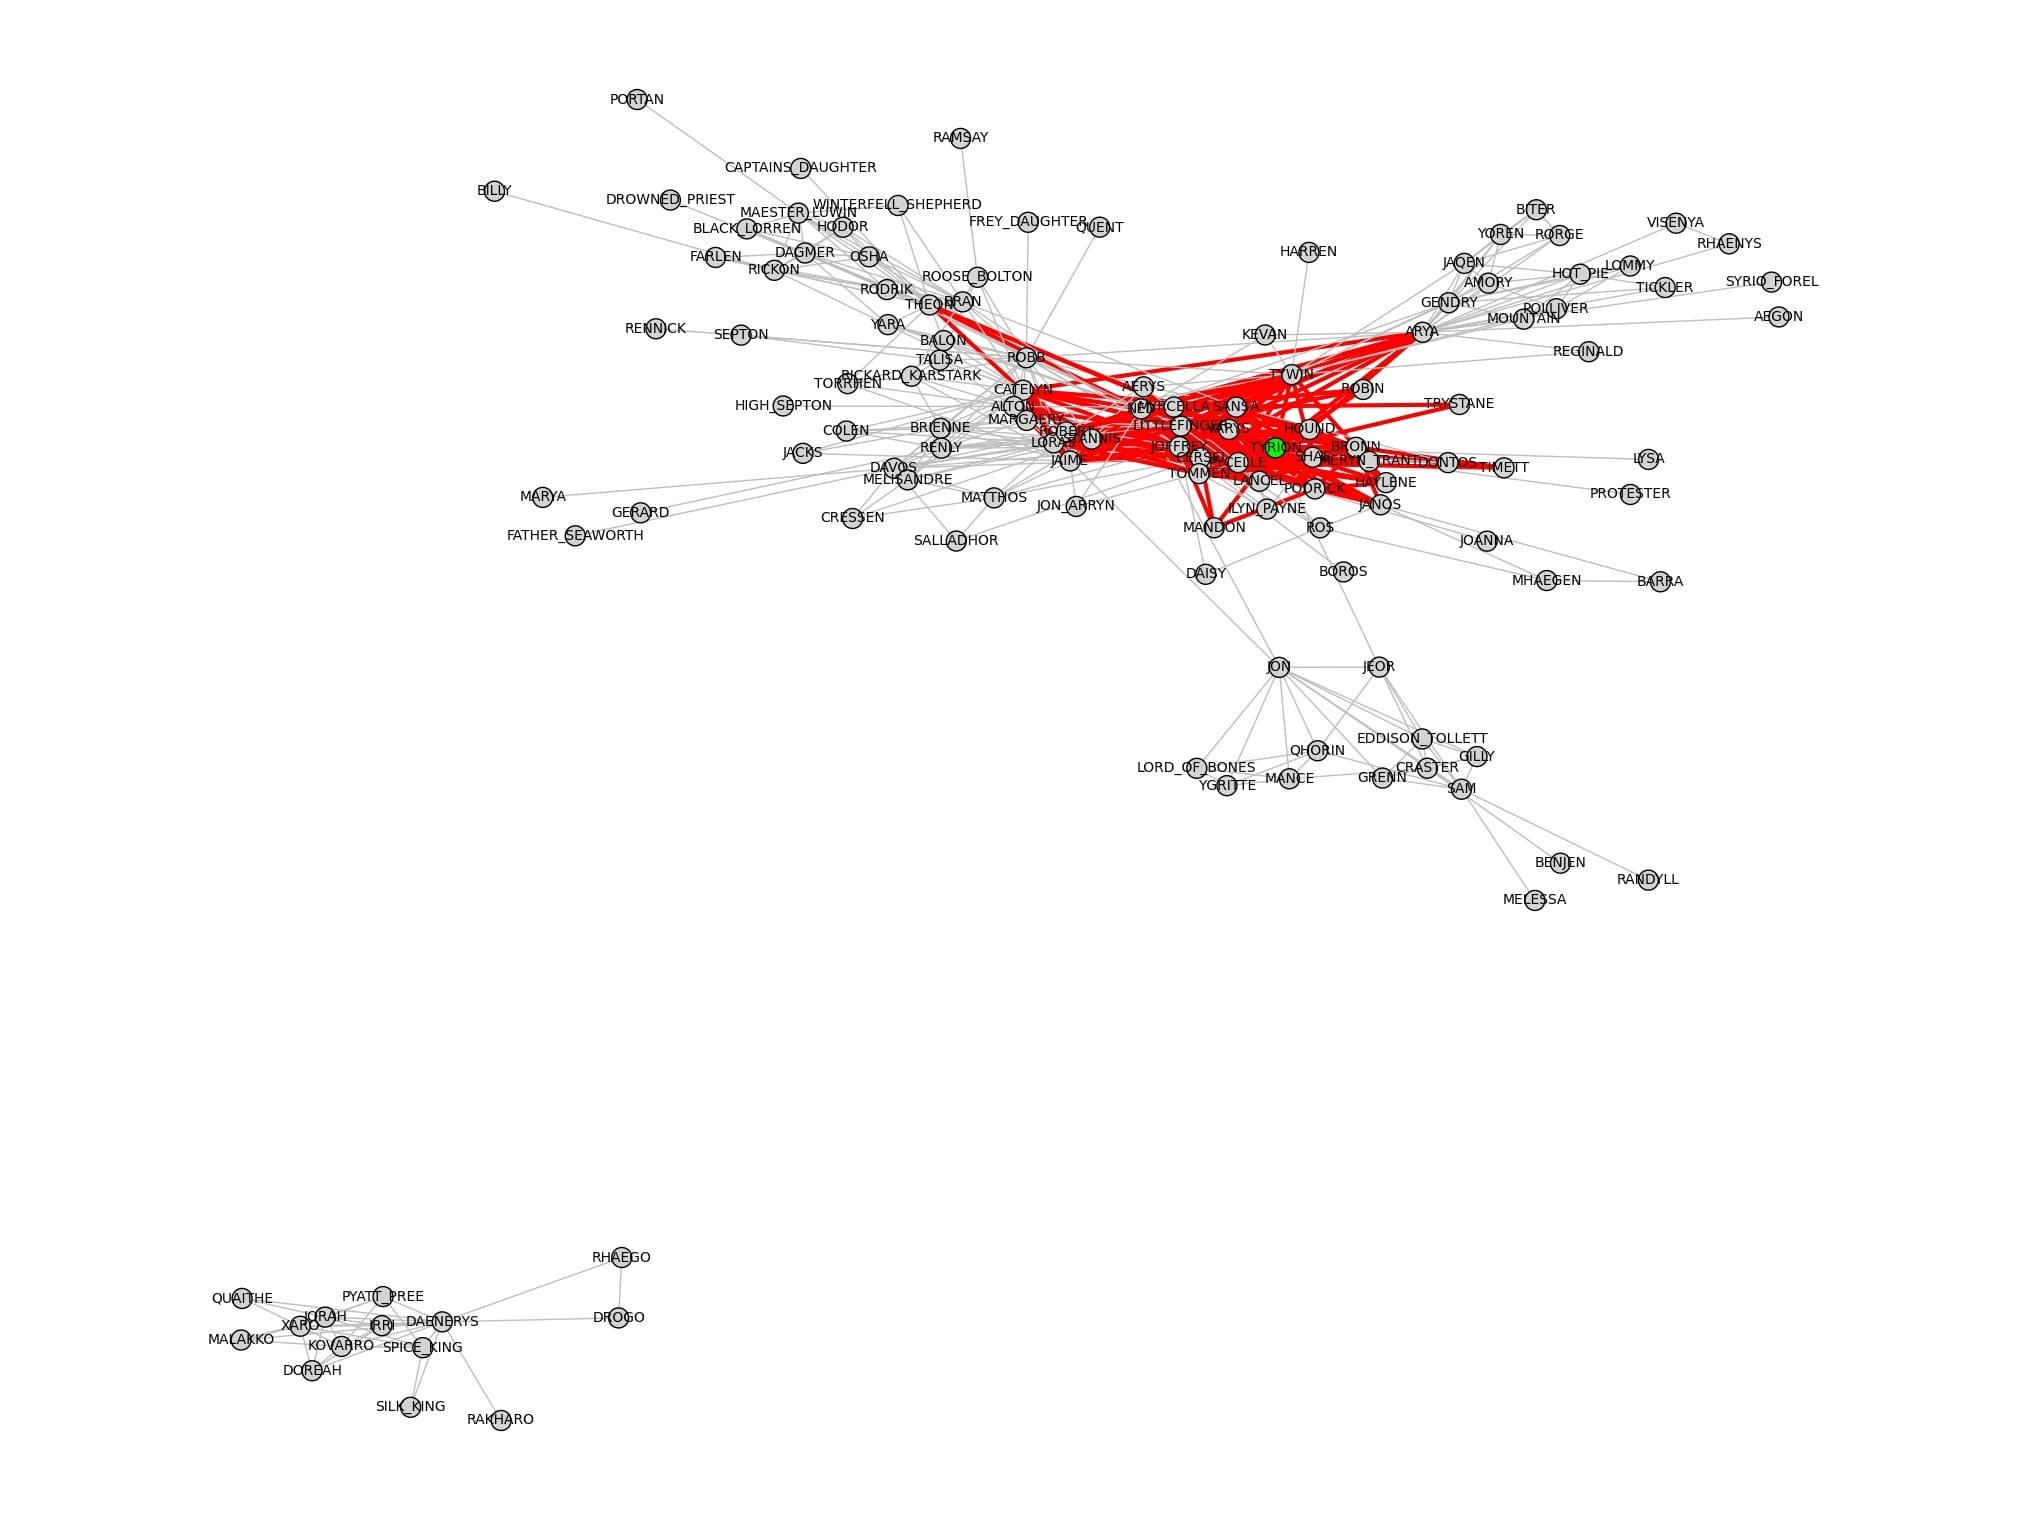
\includegraphics[width=0.5\textwidth]{img/s2/triangles_tyrion.jpg} \\
    \caption{\small{All triangles involving Tyrion Lannister in Season 2}}
\end{figure}

Interestingly, Arya holds triangles that span the communities of Harrenhall and King's Landing. Tyrion, although in this season spends a lot of time in King's Landing, is continuing to bond and form triangles in different communities. These two characters share an adventurous and independent spirit.


\subsubsection{Communities}

The story lines during Season 2 revolve around 7 main communities:

\begin{itemize}
    \item \textbf{King's Landing} (Tyrion, Joffrey, Cersei): Joffrey Baratheon holds the Iron Throne. Tyrion, which arrives in King's Landing to deal with a struggle with Renly Baratheon's claim, is the clear focus of this large community. His rival is his sister Cersei. The two interact more with each other ($weight_{c,t}=177$) than either does with Joffrey($weight_{j,c}=50$, $weight_{j,t}=79$), indicating where the true power of the Throne really resides.
    \item \textbf{Daenerys} (Daenerys, Jorah): her community is now in Essos, isolated from the rest of the characters, and is finding new allies to support her claim to the Iron Throne. The structure of this community is very simple, revolving around Daenerys.
    \item \textbf{Harenhall} (Arya, Tywin): Arya, who in season 1 got smuggled out of King's Landing after Ned Stark's death, is captured with other people and brought to Harrenhal. Lord Tywin Lannister returns to the castle, and immediately realizes that Arya is a girl posing as a boy. She claims that it made it safer to travel. Tywin commends her intelligence and makes her his cupbearer ($weight_{t,a}=103$). 
    Interestingly, Arya and Tywin are both hubs, although their roles are very different: Arya ties the community together, whereas Tywin connects the community with other communities, particularly with King's Landing.
    \item  \textbf{Stormlands and Riverlands} (Catelyn, Robb, Stannis, Jamie): The Riverlands and Stormlands community is the most cumbersome, reflecting the uneasy coalitions and rivalries that have erupted due to the deaths of Ned and King Robert. Catelyn glues this community together, as she tries to negotiate these would-be kings behind a common cause.
    \item  \textbf{The Far North} (Jon, Sam):  In the distant north, the Night's Watch has mounted an expedition beyond the Wall, searching for missing rangers and investigating rumors of wildlings gathering in the mountains. The Far North organizes around Jon Snow, with particularly strong ties to Ygritte ($weight_{j,y}=110$) and Qhorin ($weight_{j,q}=71$).
    \item  \textbf{Iron Islands and Winterfell} (Theon, Bran): Theon and his men seize the poorly defended Winterfell. He forces Bran Stark ($weight_{t,b}=47$) to yield to him by threatening his people. 
    
\end{itemize}

\newpage

\begin{figure}[!h]
    \centering
    \textbf{Infomap}  \\
    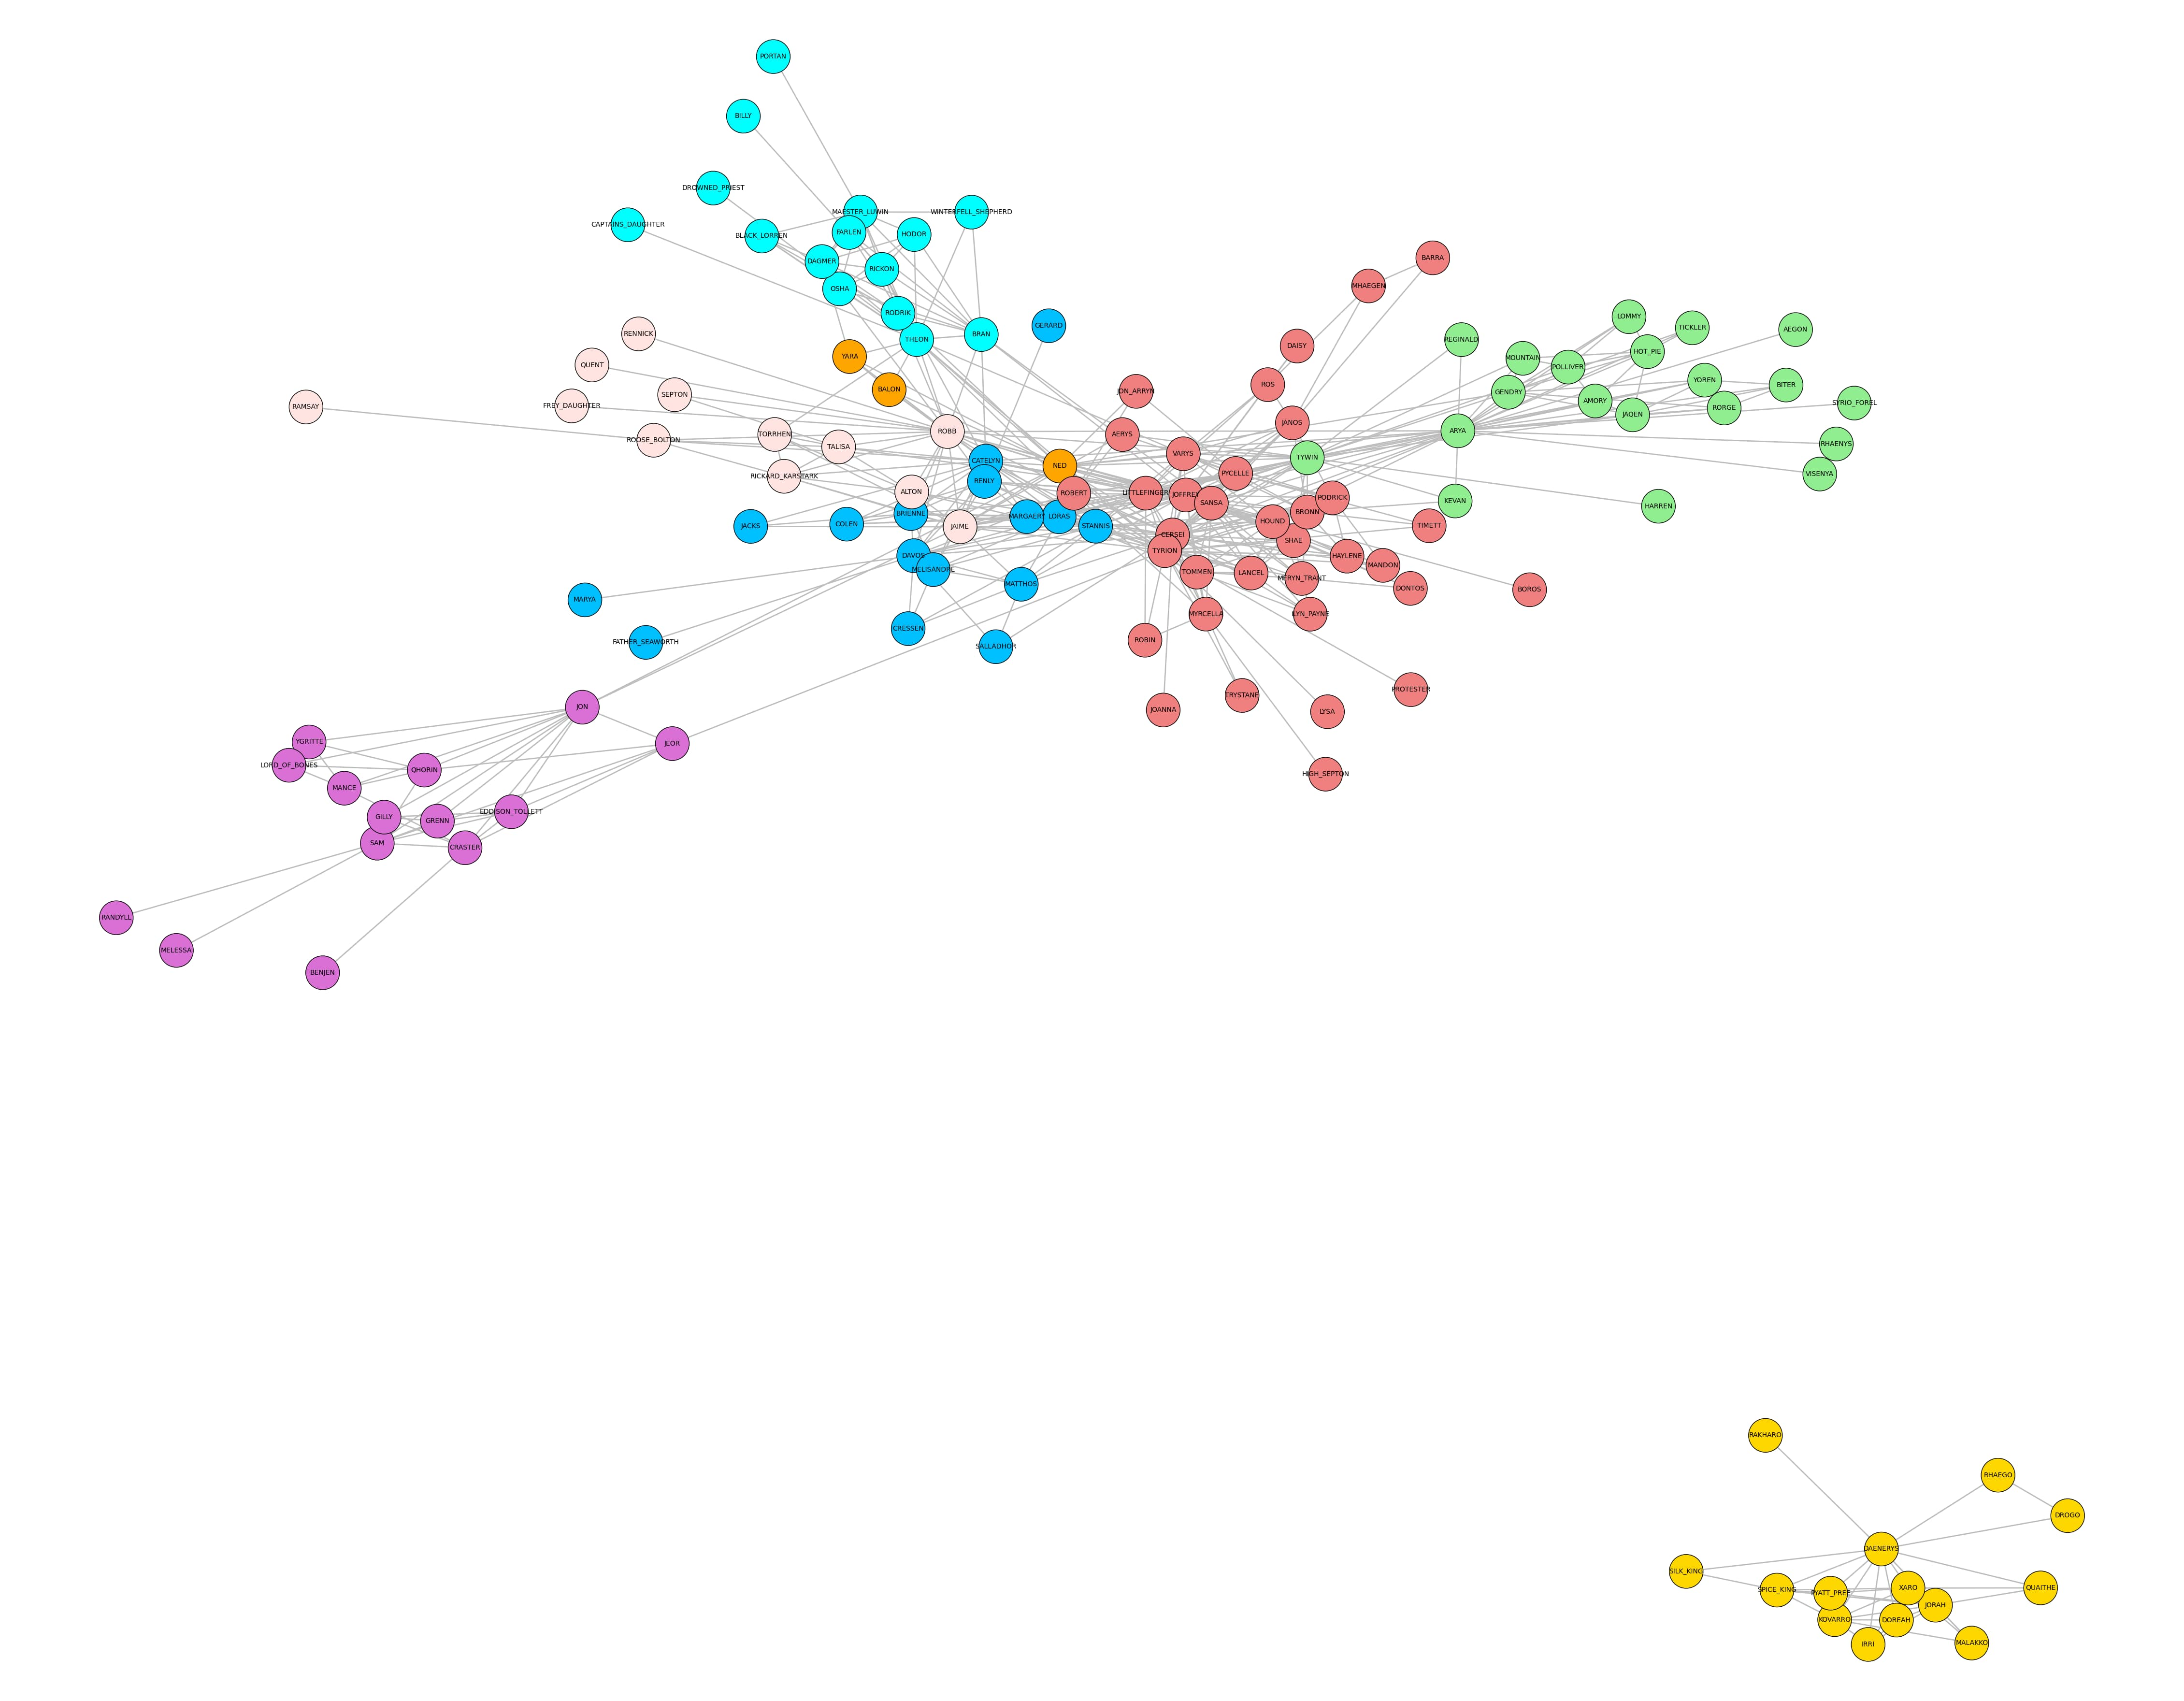
\includegraphics[width=0.5\textwidth]{img/s2/communities_infomap.jpg}
    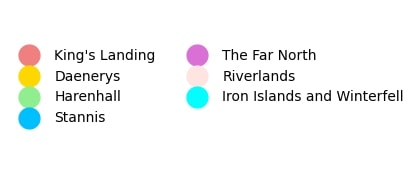
\includegraphics[width=0.3\textwidth]{img/s2/infomap_legend.jpg}\\
    \caption{\small{$\#communities=8$, $modularity=0.561$}}
    \label{fig:infomap_s2}
\end{figure}


\begin{figure}[!h]
    \centering
    \textbf{Girvan-Newman} \\
    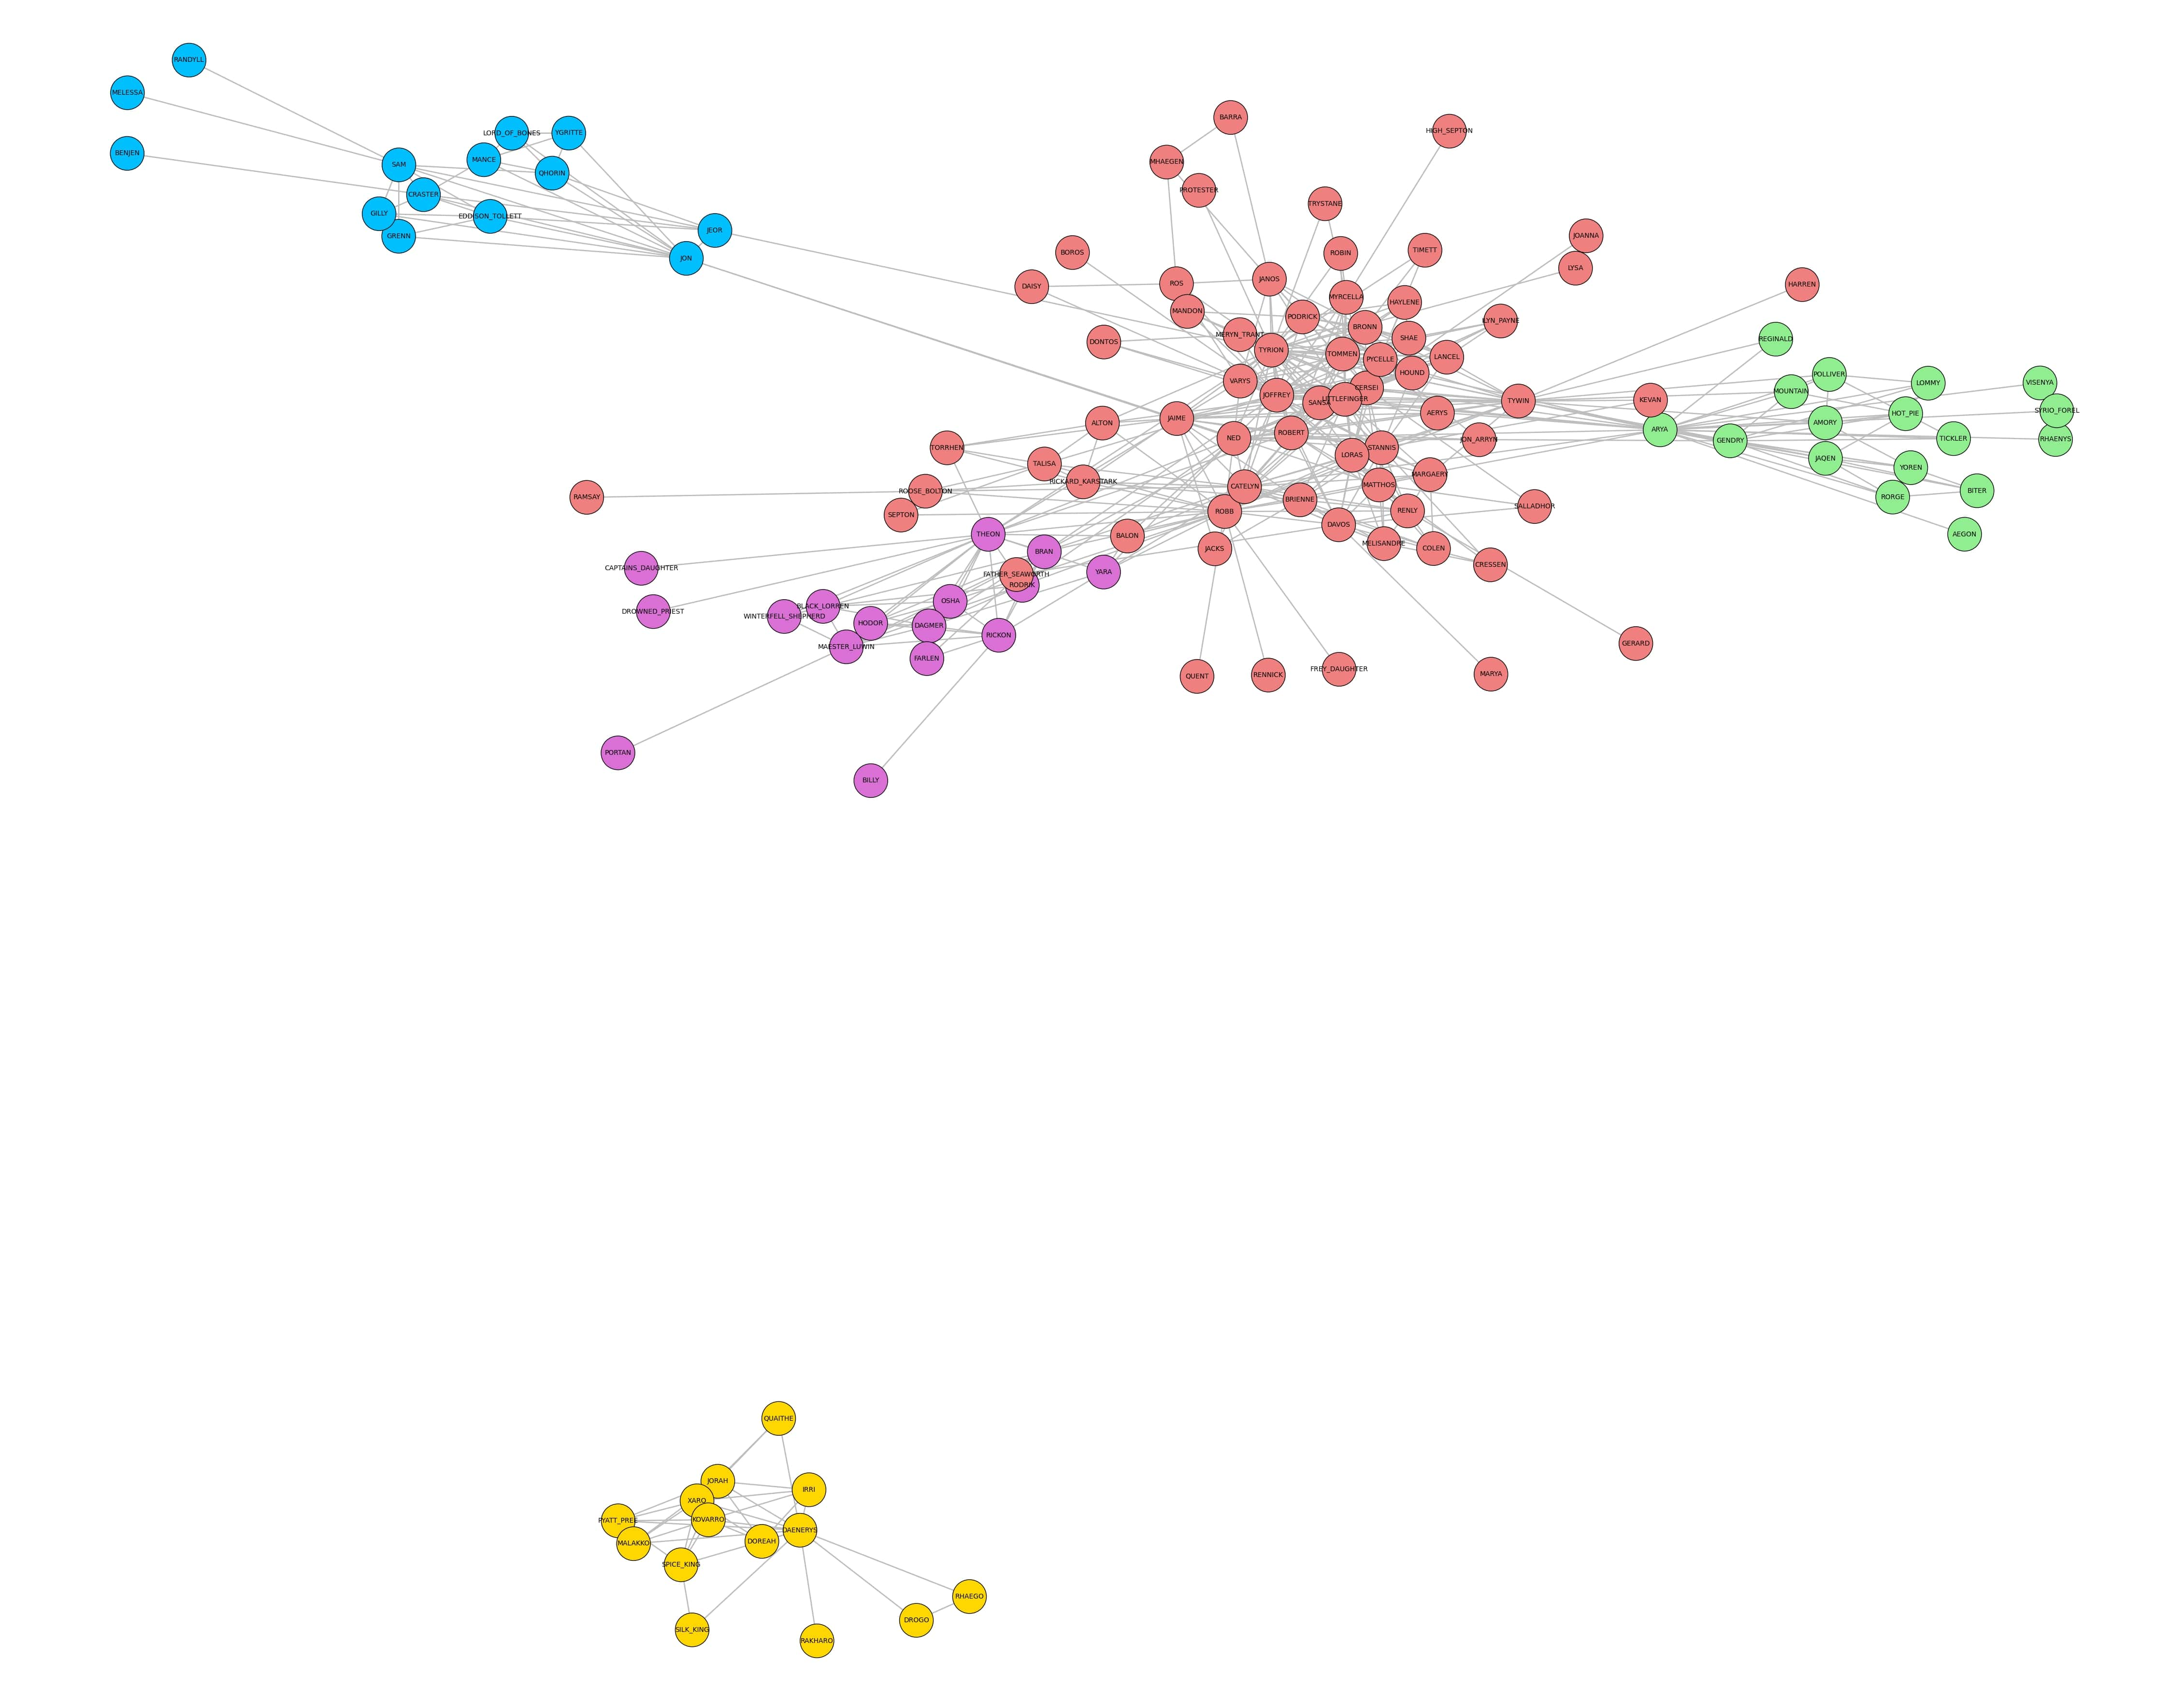
\includegraphics[width=0.5\textwidth]{img/s2/communities_g-n.jpg}
    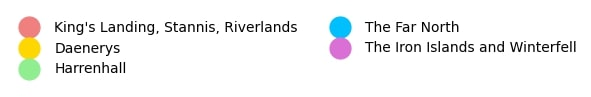
\includegraphics[width=0.45\textwidth]{img/s2/g-n_legend.jpg}\\
    \caption{\small{$\#communities=5$, $modularity=0.477$}}
    \label{fig:gn_s2}
\end{figure}

\vspace{5cm}


\begin{figure}[!h]
    \centering
    \centering
    \textbf{Louvain} \\
    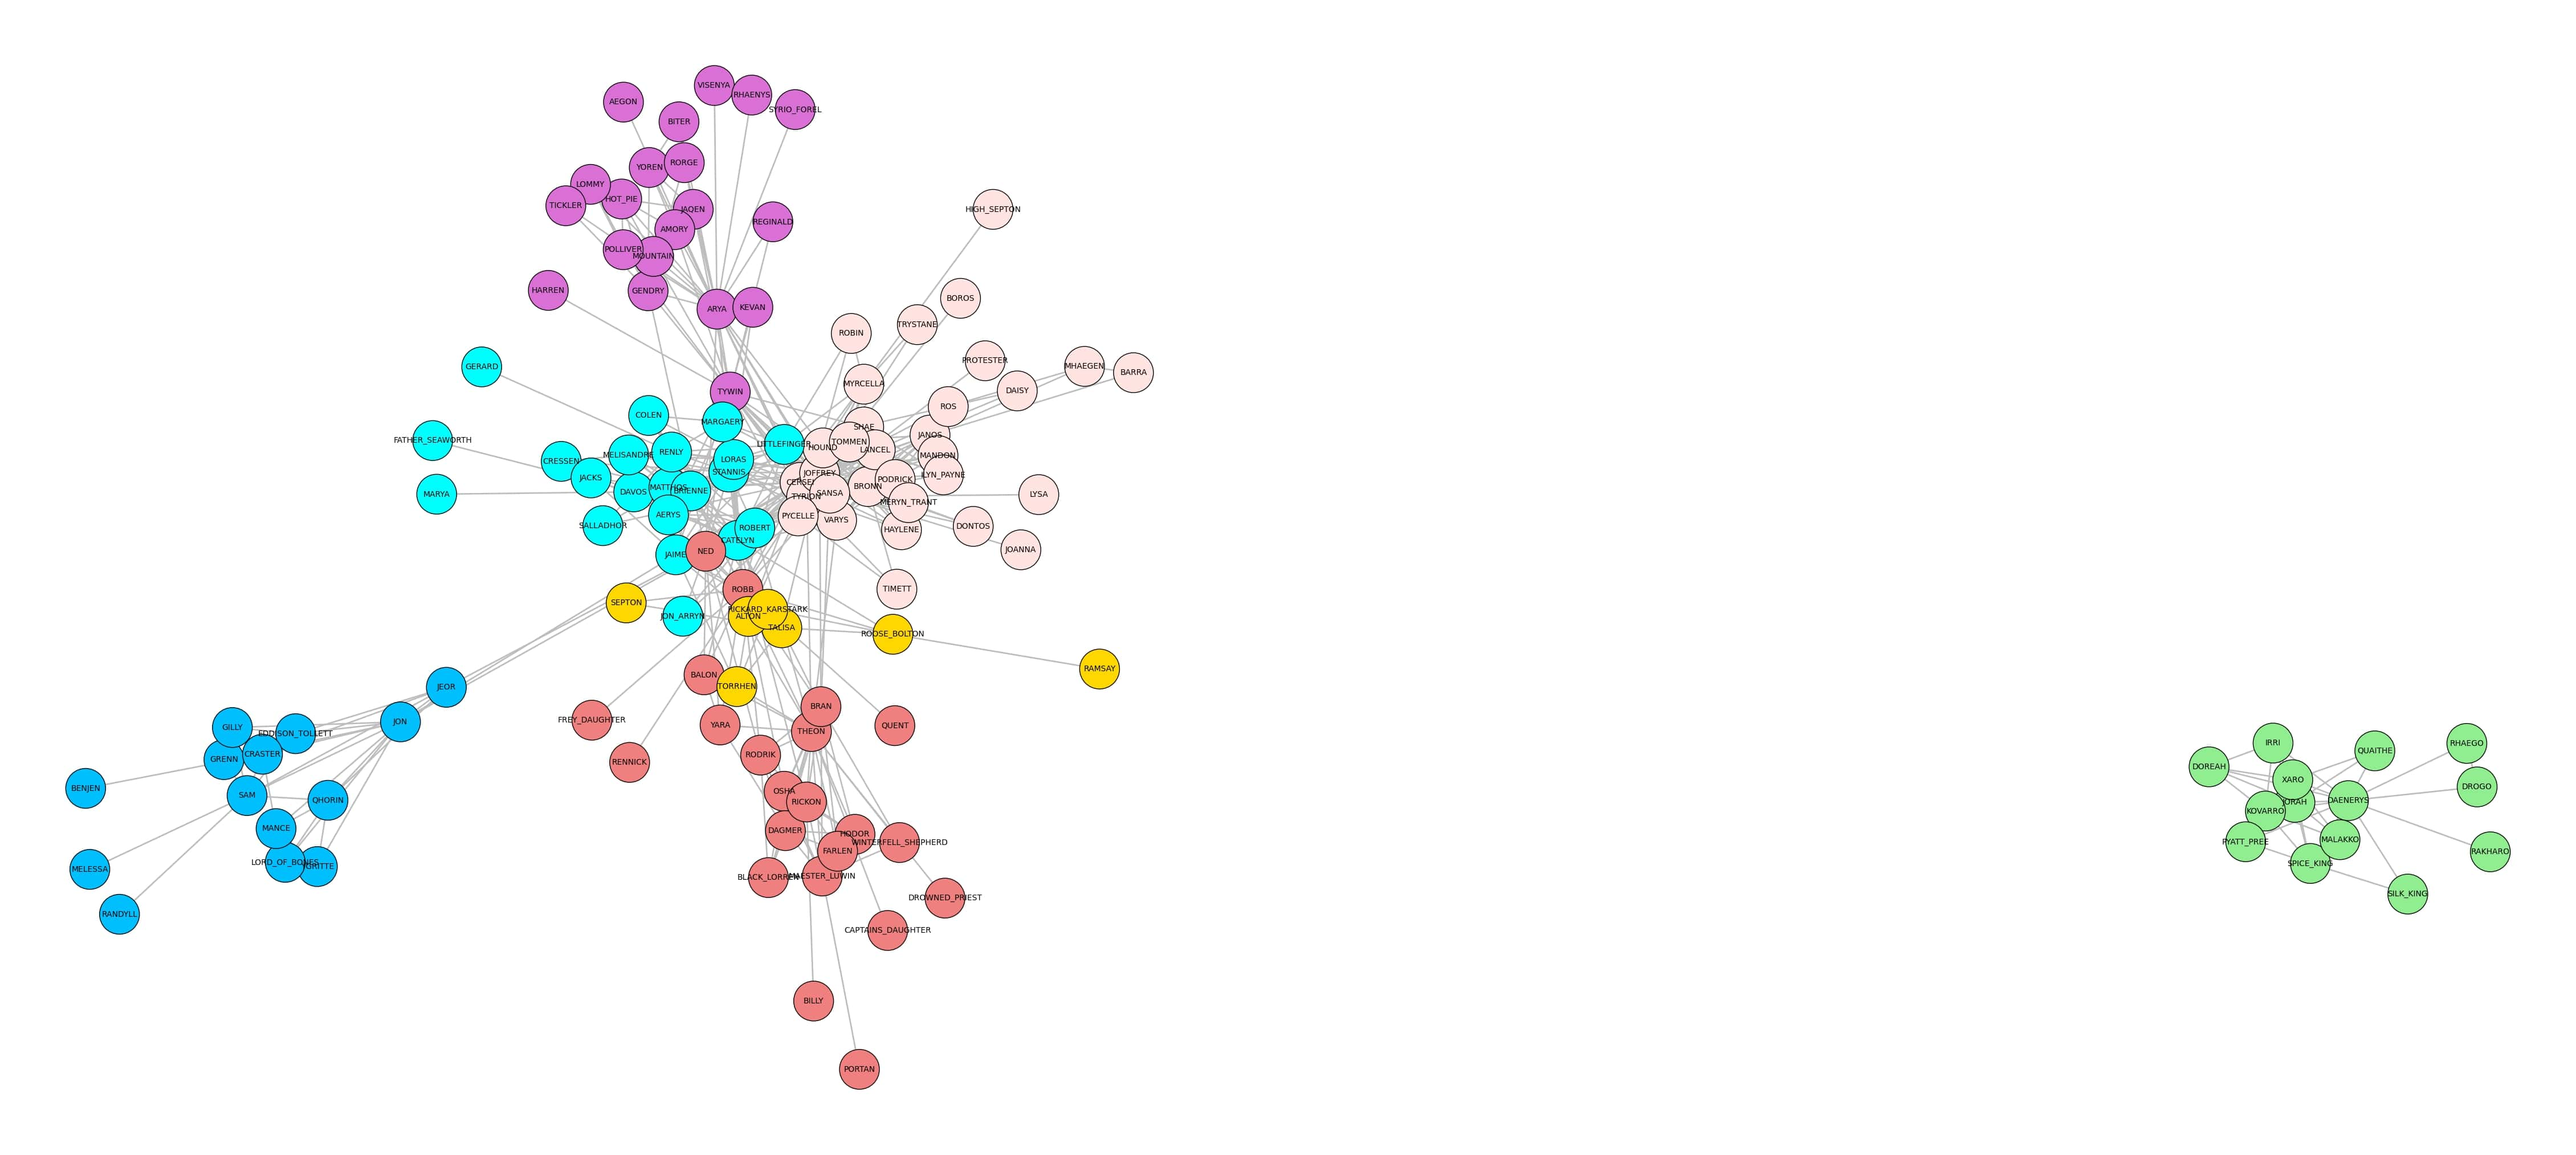
\includegraphics[width=0.45\textwidth]{img/s2/communities_louvain.jpg}
    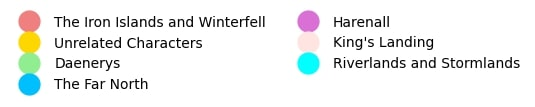
\includegraphics[width=0.35\textwidth]{img/s2/louvain_legend.jpg}\\
    \caption{\small{$\#communities=7$, $modularity=0.563$}}
    \label{fig:louvain_s2}
\end{figure}    

\begin{figure}[!h]
    \centering
    \textbf{Greedy Modularity Maximization}\\
    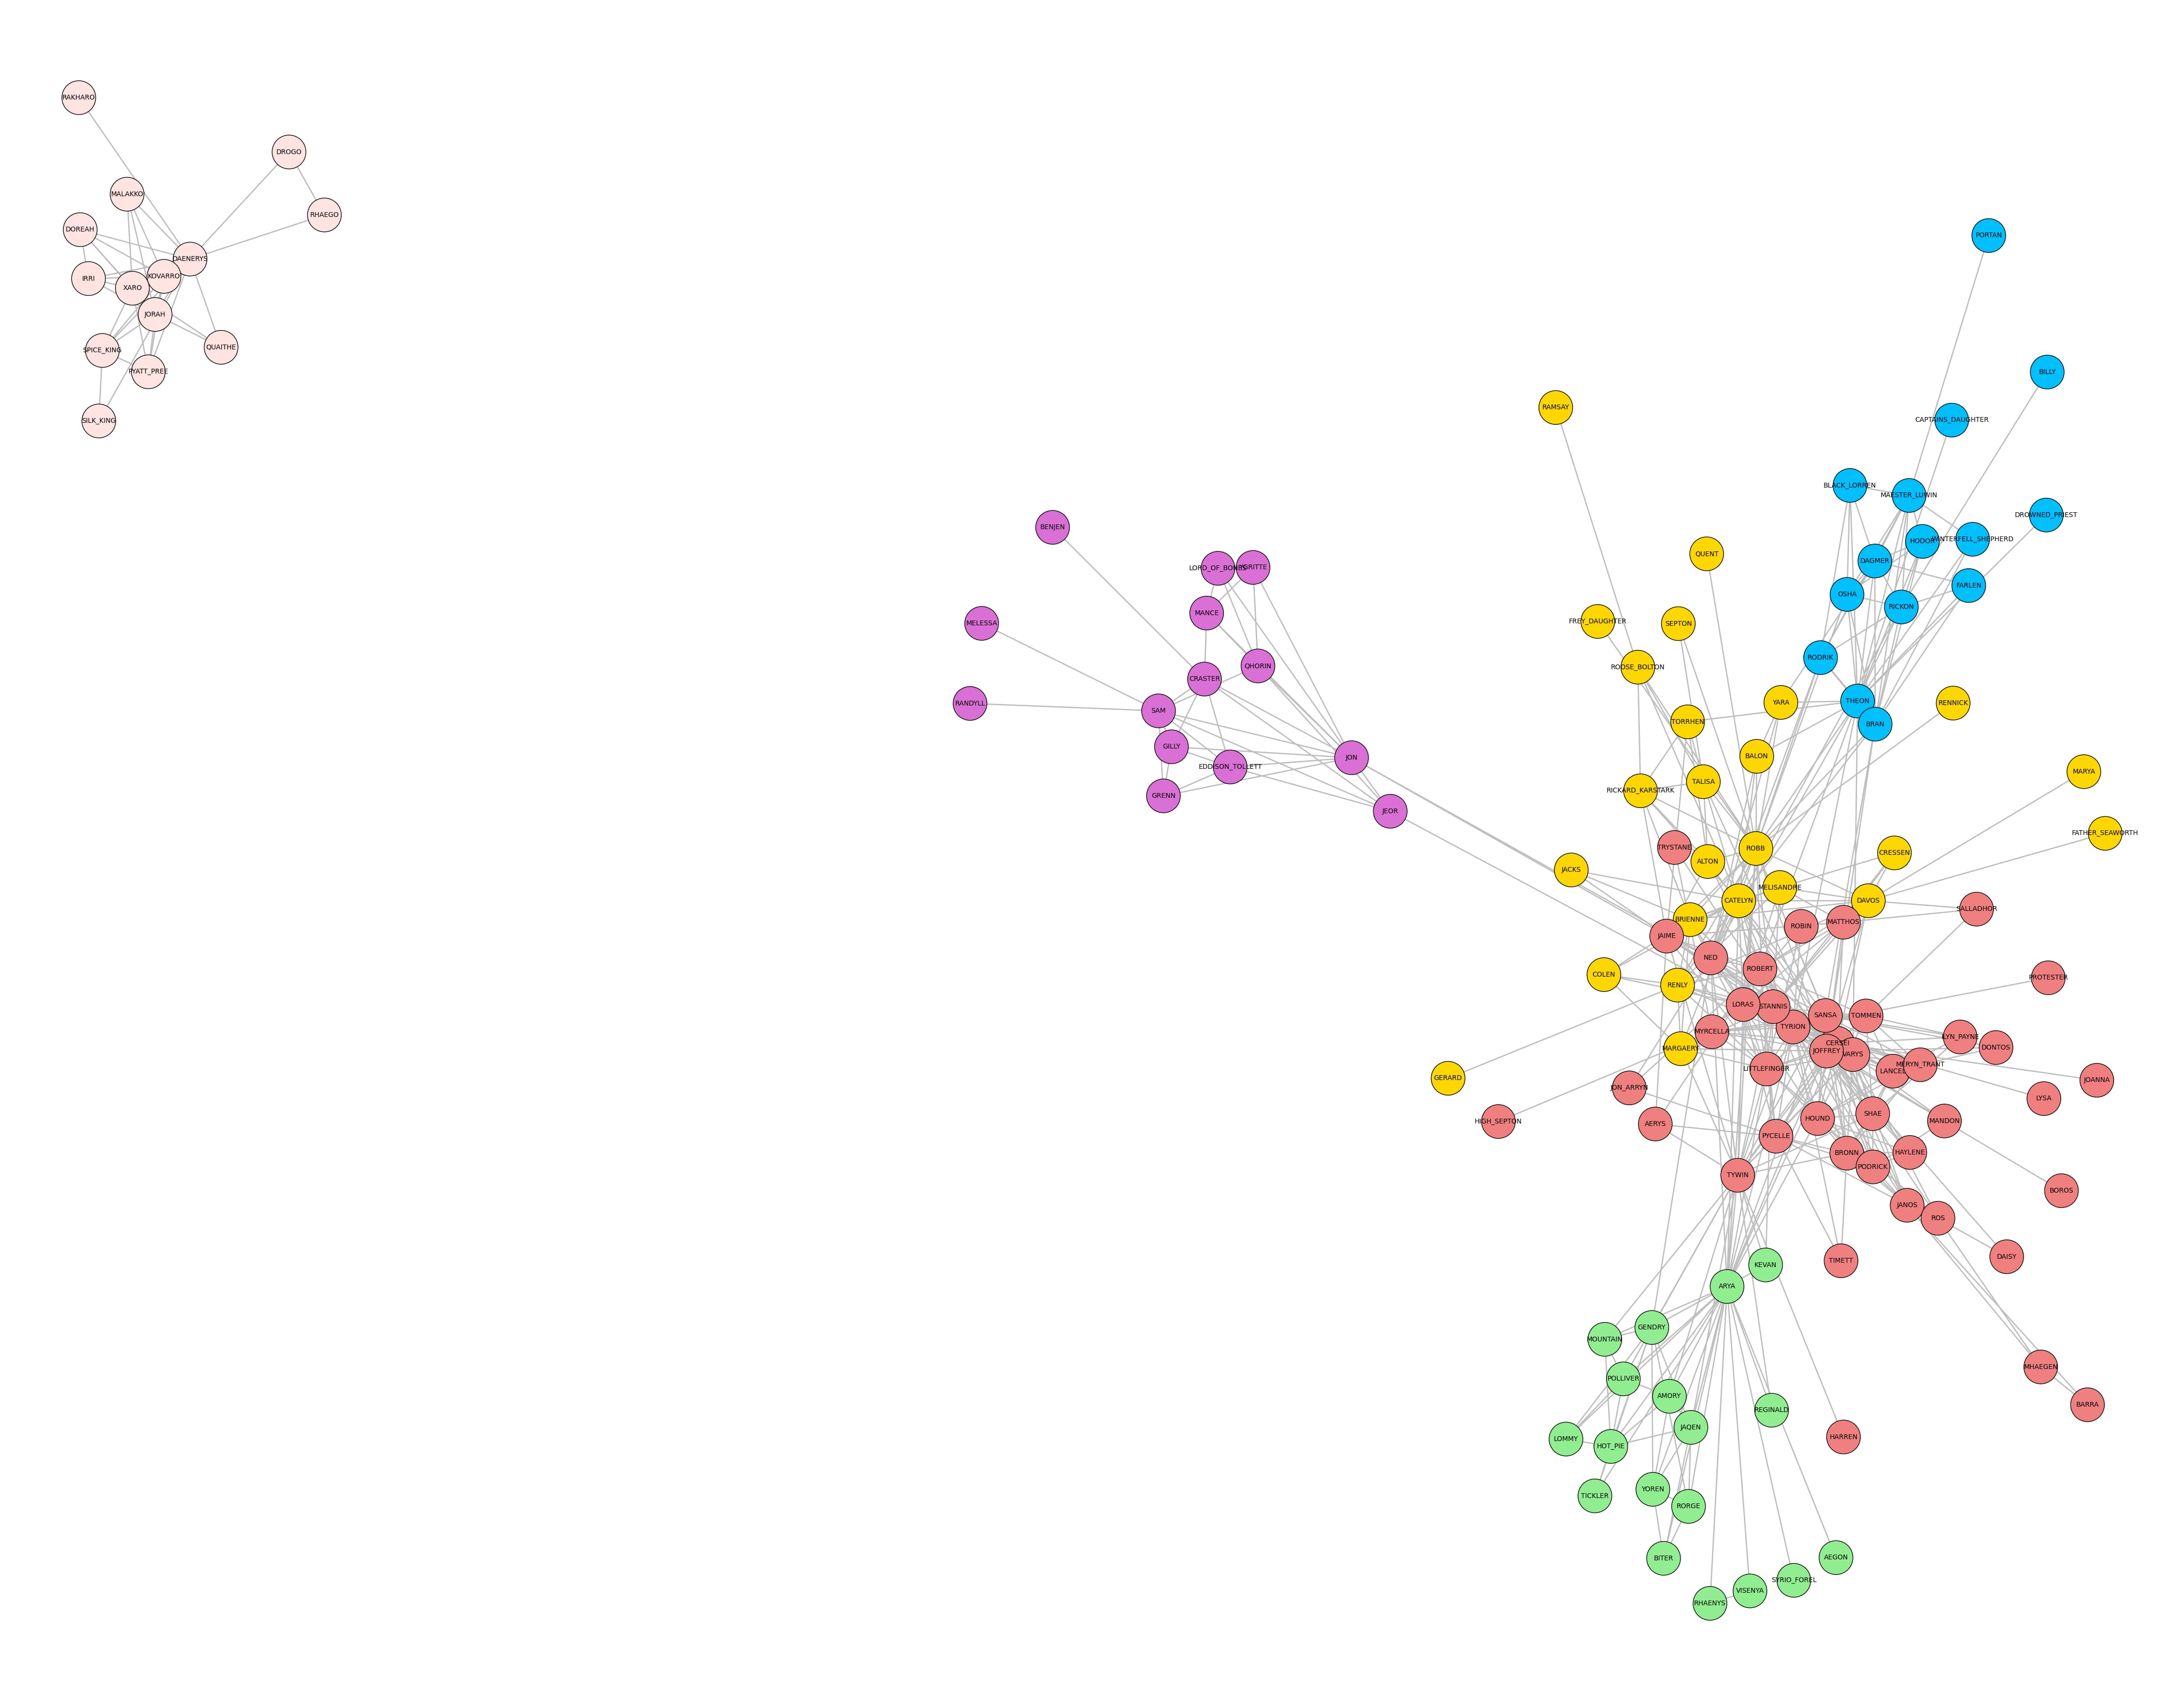
\includegraphics[width=0.4\textwidth]{img/s2/communities_gmm.jpg}
    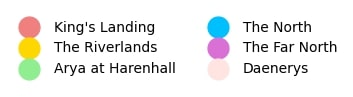
\includegraphics[width=0.27\textwidth]{img/s2/gmm_legend.jpg}\\
    \caption{\small{$\#communities=6$, $modularity=0.532$}}
    \label{fig:gmm_s2}
\end{figure}

\begin{figure}[!h]
    \centering
    \textbf{Spectral Clustering}
    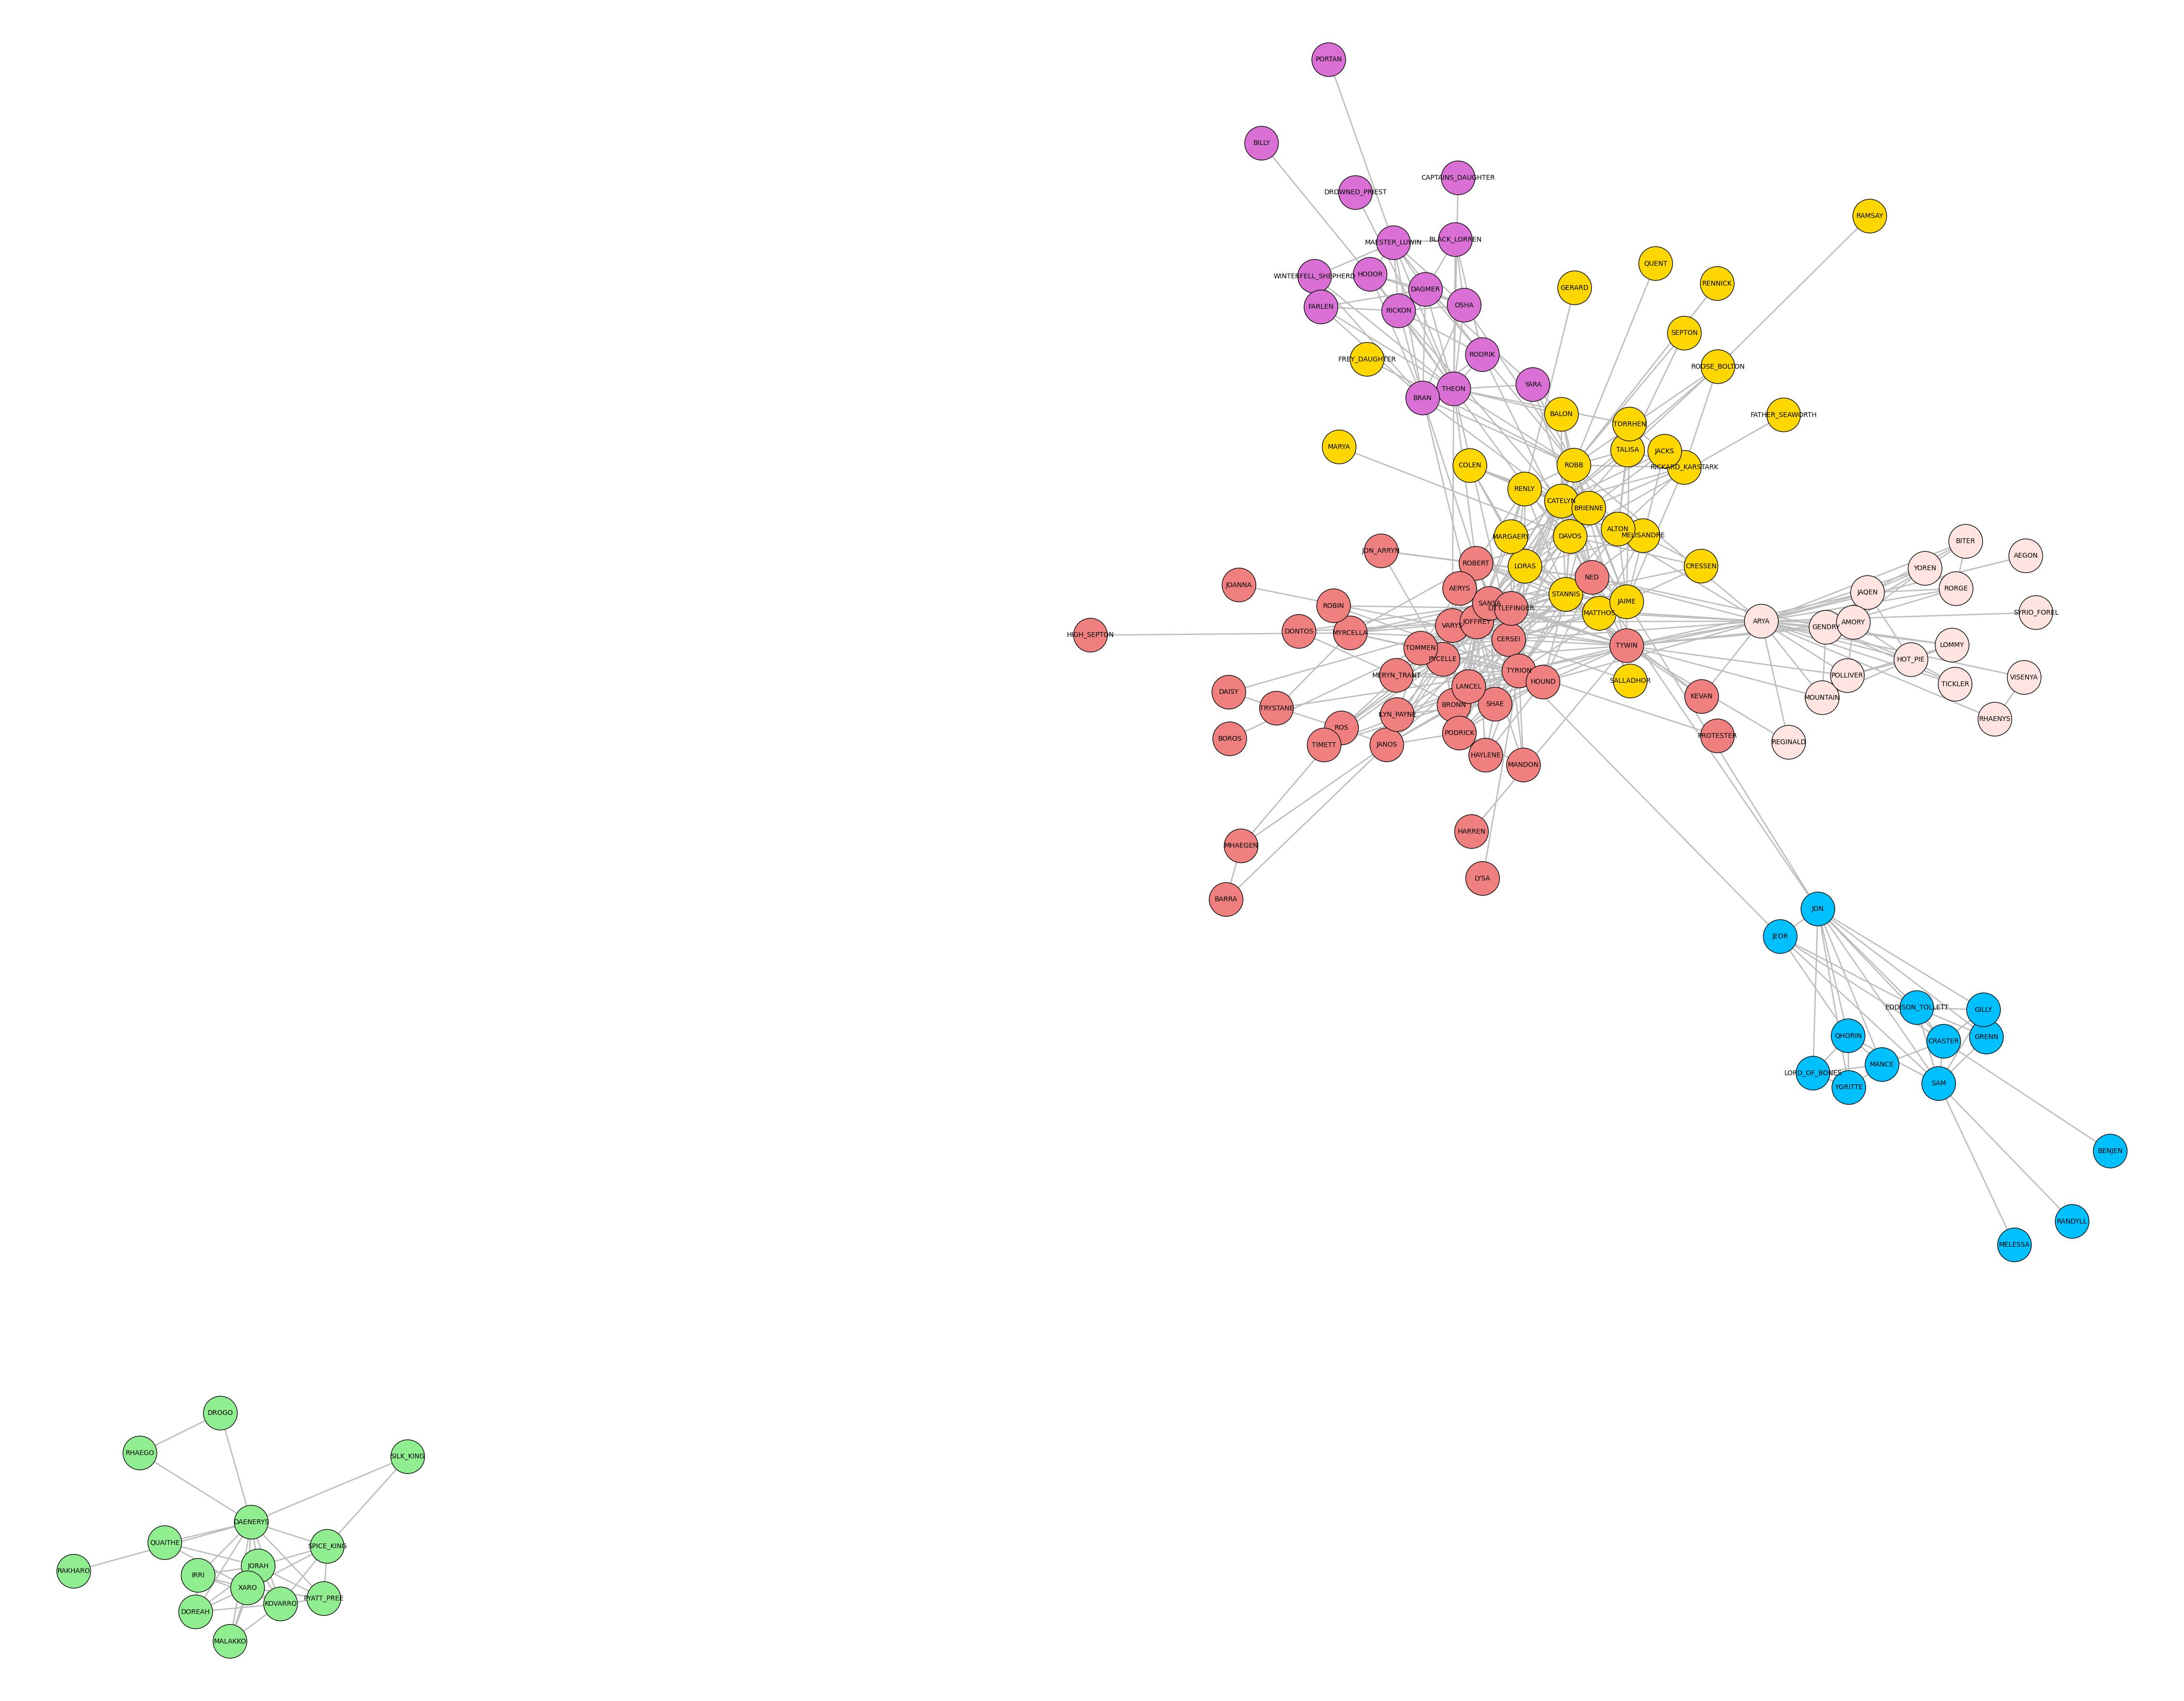
\includegraphics[width=0.35\textwidth]{img/s2/communities_sc.jpg}
    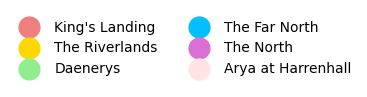
\includegraphics[width=0.3\textwidth]{img/s2/sc_legend.jpg}\\
    \caption{\small{$\#communities=6$, $modularity=0.557$}}
    \label{fig:sc_s2}
\end{figure}




\paragraph{Comparison Between Methods}

Below, the various community detection methods are compared with respect to performance on Season 2's graph.

\begin{figure}[!h]
    \centering
    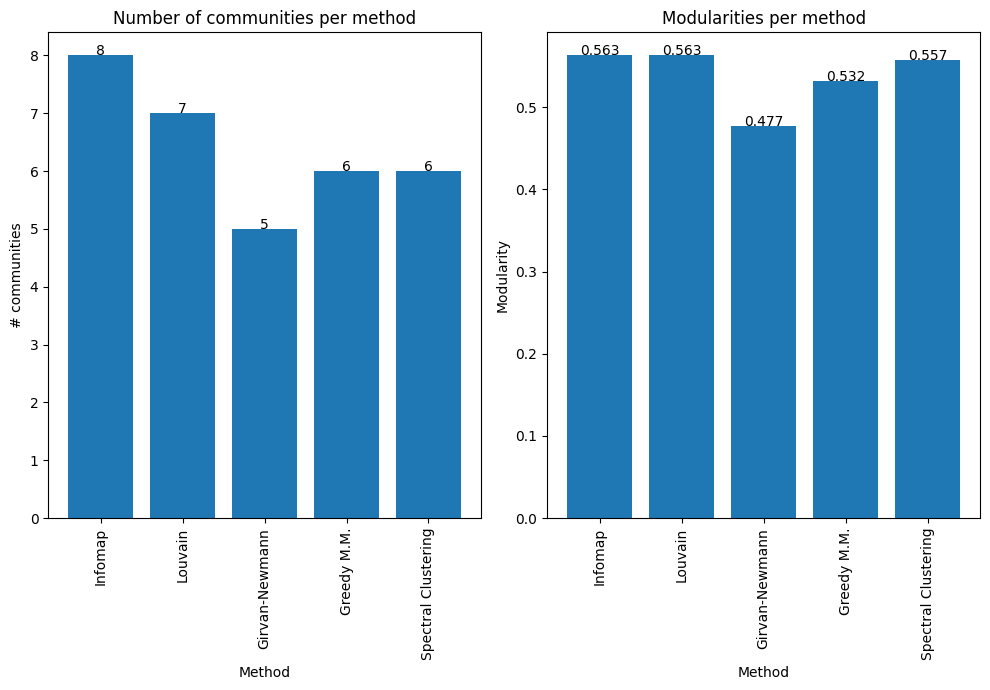
\includegraphics[width=0.45\textwidth]{img/s2/communities_comparison.jpg} \\
    \label{fig:comm_comp_s2}
\end{figure}

\textbf{Infomap}\textsuperscript{\ref{fig:infomap_s2}} is able to detect all 7 communities as described above, with a modularity score of 0.559. 

\textbf{Girvan-Newman}\textsuperscript{\ref{fig:gn_s2}} struggles to find communities that are more subtle and not evident at first sight. Indeed, it is able to recognize well clustered communities such as Daenerys, Harrenhall and the Far North, but it is not capable of distinguishing more tightly aggregated ones, for example the ones intrinsically close to King's Landing.

\textbf{Louvain}\textsuperscript{\ref{fig:louvain_s2}} is able to recognize 7 communities, which are similar to the ones Infomap detected. The modularity score is 0.563. However, while Infomap is able to distinguish the two, Louvain groups the Riverlands and the Stormlands together, which is totally plausible and arguably the right choice. This community is the most unwieldy, reflecting the uneasy coalitions and rivalries that have erupted due to the deaths of Ned and King Robert. 
Besides this, there is also a small community of secondary characters that is closely involved with Robb Stark, who is however not clustered in this community, and with the Boltons. It could be that, since the Boltons are currently not particularly involved with the storylines of the North or with King's Landing, Louvain decided to generate a new cluster, though not really significant.

\textbf{Greedy Modularity Maximization}\textsuperscript{\ref{fig:gmm_s2}} is able to detect 6 communities, which roughly correspond to Louvain's findings, and reaches a modularity score of 0.532. Though, there are two considerations that are worth mentioning; as said before, Arya's community in Harrenhall also comprised of Tywin Lannister, who was connecting Harrenhall with King's Landing. Here instead Tywin is part of the King's Landing community, which makes sense since he is still a major character of the Lannister family, although being physically at Harrenhall. Same goes for Jamie, who although being very close to Robb and Catelyn, is still clustered into King's Landing. Stannis is also in the same community, but should probably be in the Stormlands one.

\textbf{Spectral Clustering}\textsuperscript{\ref{fig:sc_s2}} finds the same communities as Greedy Modularity Maximization, with a slightly higher 0.557 modularity score.

Overall, Infomap and Louvain are the best performing community detection methods in this season.



\subsection{Season 3}

\begin{figure}[!h] 
    \centering
    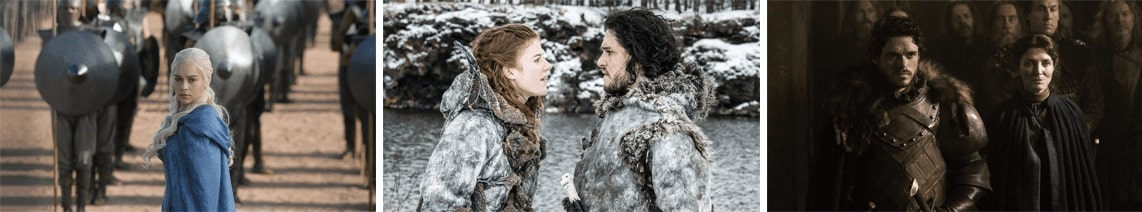
\includegraphics[width=0.48\textwidth]{img/s3/frames_s3.jpg}
\end{figure}

\begin{table}[!h]
    \centering
    \small
    \begin{tabular}{c|c}
        Description & Value  \\
        \hline
        Nodes & 124 \\
        Edges & 504 \\
        Graph Density & 0.066 \\
        Connected Graph & Yes \\
        Number of Components & 1 \\
        Small-World Network & Yes ($\lambda=1.27$ , $\gamma=10.36$) \\
        Diameter & 7 \\
        Avg. Shortest Path & 3.26 \\
        Avg. Degree & 8.13 [1,31] \\
        Most Freq. Degree & 2 \\
        Number of Bridges & 14 \\
        Deg. Assortativity Coeff. & -0.056\\
        Global Clustering Coeff. & 0.481 \\
        Average Clustering Coeff. & 0.597 \\
        \hline 
    \end{tabular}
    \vspace{0.2cm}
    \caption{Summary table for Season 3's network}
    \label{tab:my_label}
\end{table} 

\begin{figure}[!h]
    \centering
    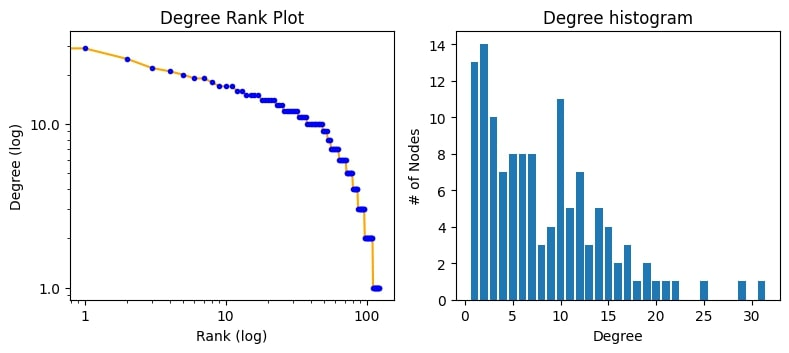
\includegraphics[width=0.5\textwidth]{img/s3/degree_plot.jpg}
    \caption{\small{Degree distribution of Season 3's network}}
\end{figure}

\subsubsection{Centrality}

Below we plot Season 3’s interaction network where the node sizes are scaled according to PageRank centrality, and the layout is computed using the Fruchterman-Reingold force-directed layout algorithm.

\newpage

\begin{figure}[!h]
    \centering
    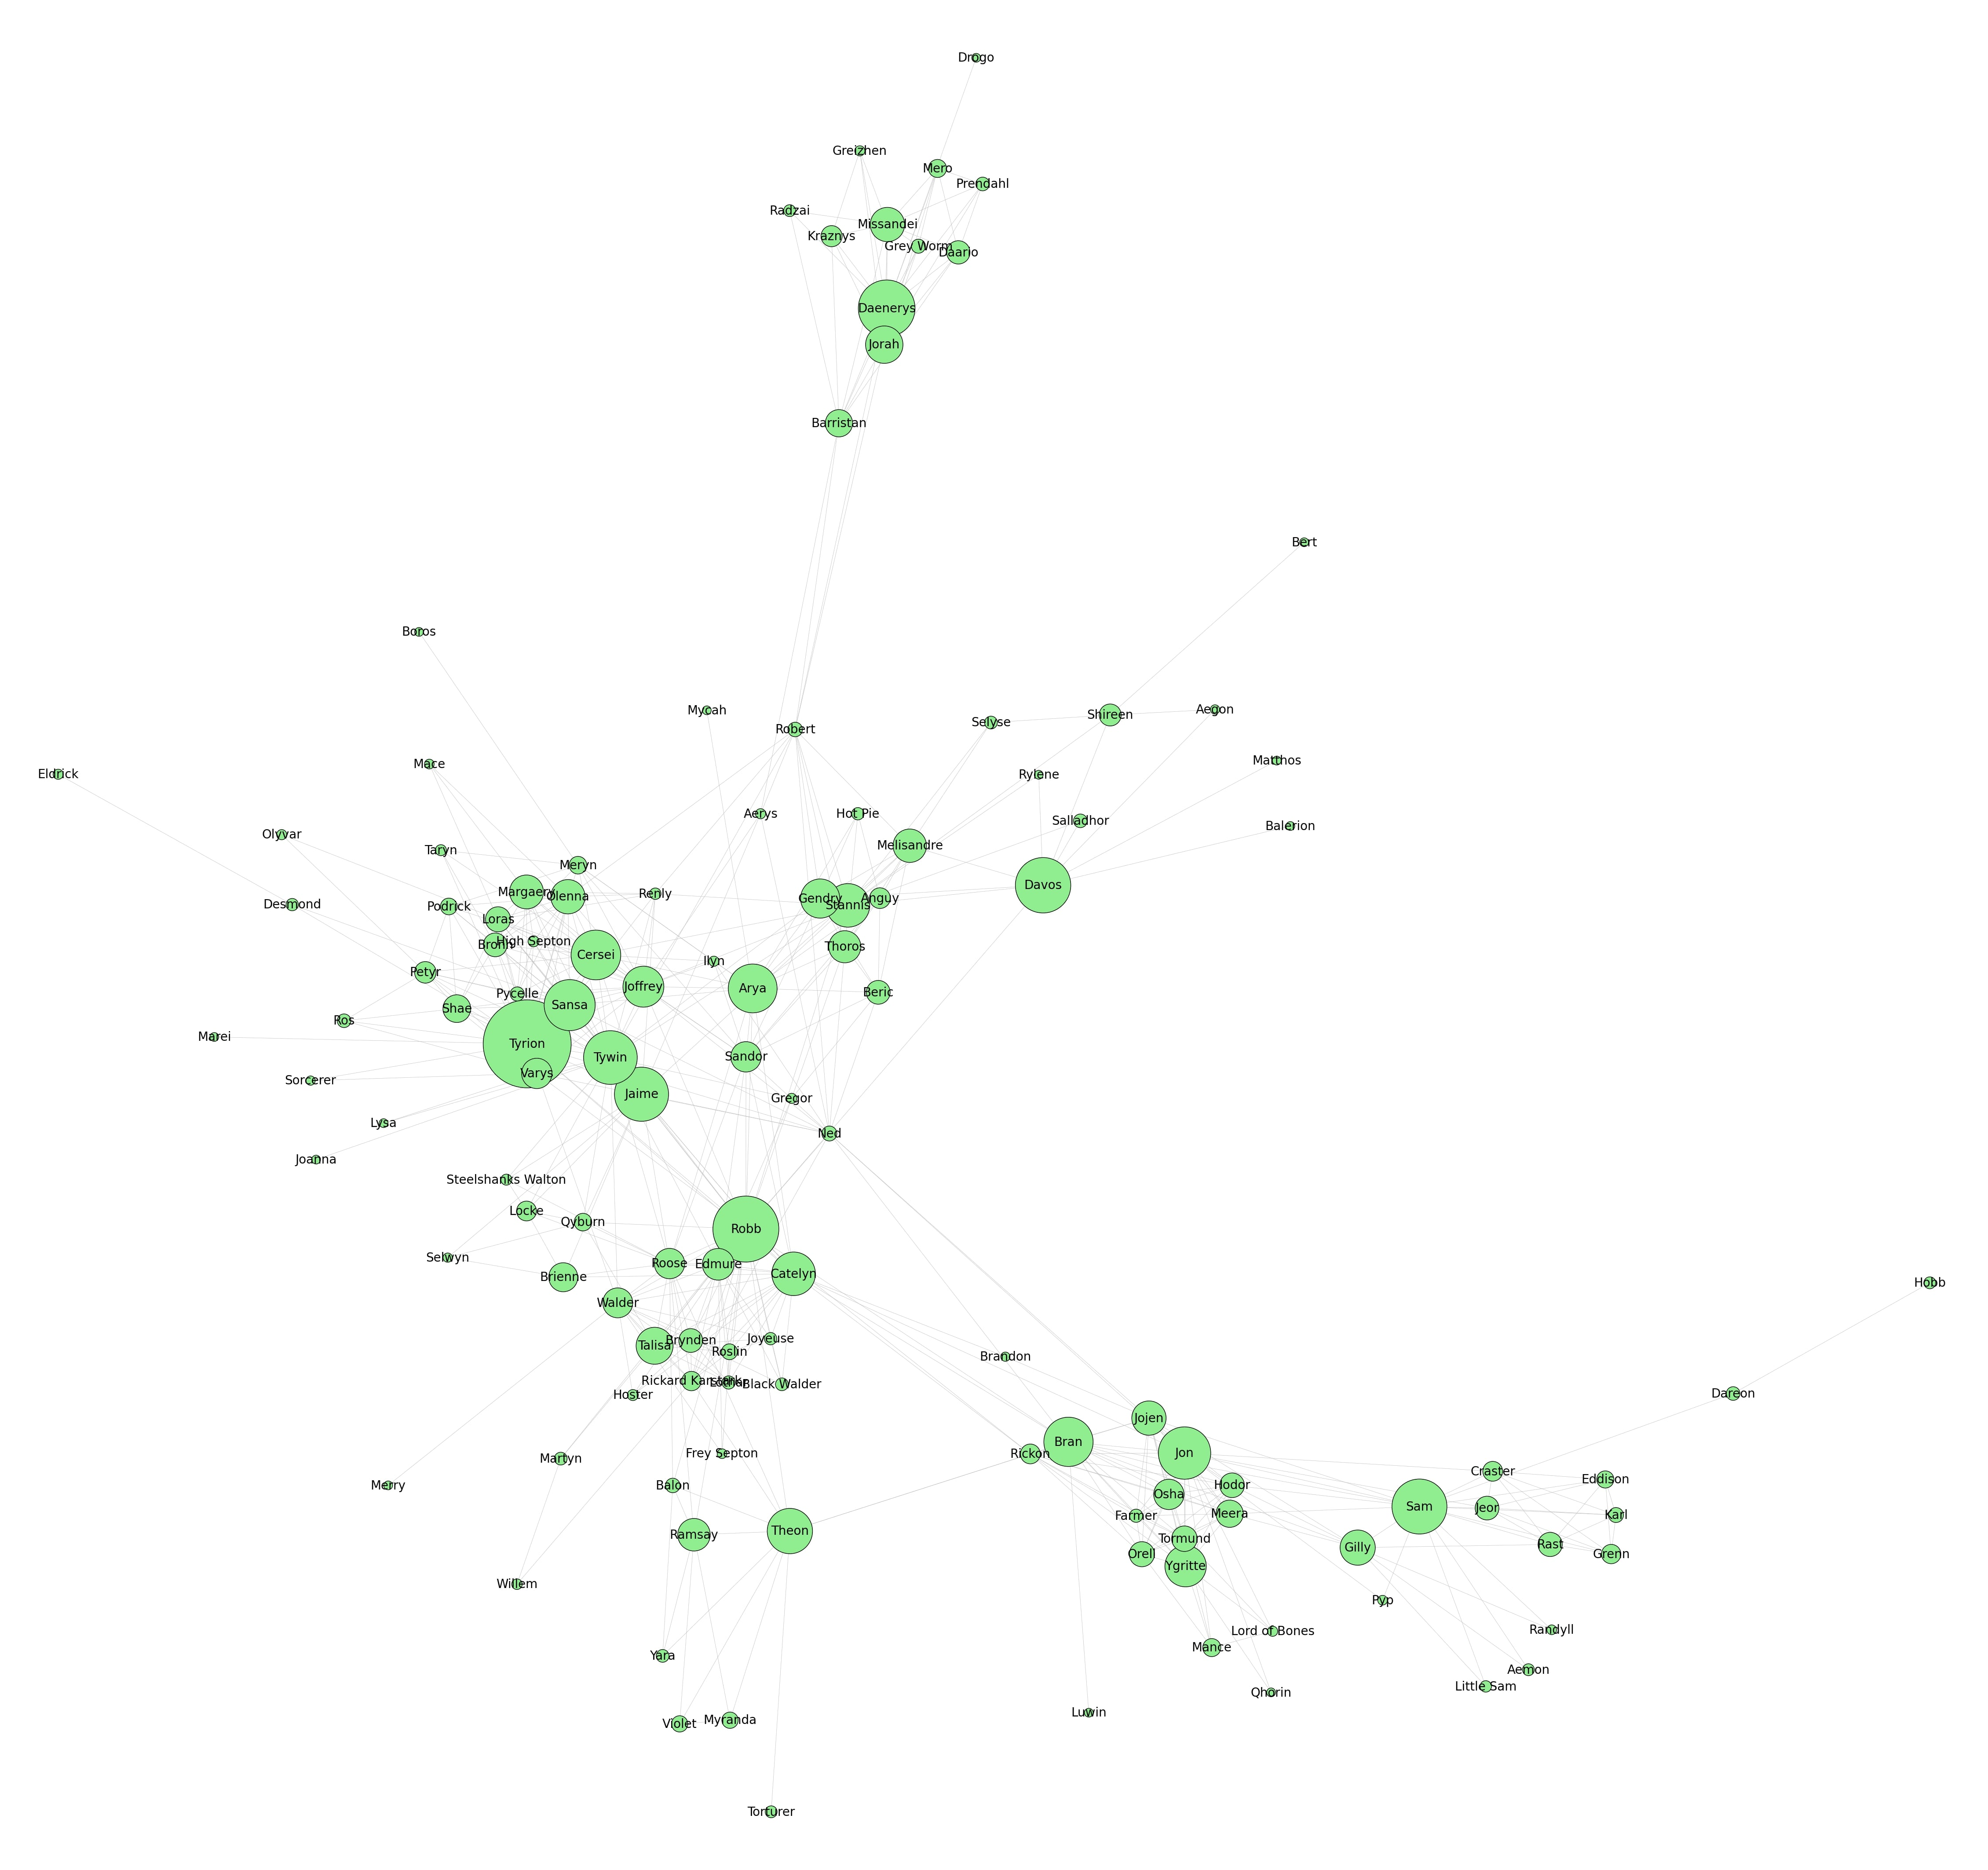
\includegraphics[width=0.4\textwidth]{img/s3/pagerank_network.jpg}
\end{figure}

In the tables\textsuperscript{\ref{tab:cent_s2}, \ref{tab:cent_means_s2}} on the right side show the results obtained by the different centrality measures are reported.

\begin{table}[!h]
    \centering
    \small
    \begin{tabular}{c|c|c}
        Measure & Character & \small{Highest Centrality Score} \\
        \hline
                    & Robb & 0.238 \\
                    & Ned & 0.175 \\
        Betweenness & Robert & 0.161 \\
                    & Bran & 0.148 \\
                    & Jon & 0.136 \\
        \hline 
                    & Robb & 0.479 \\
                    & Ned & 0.456 \\
        Closeness   & Catelyn & 0.452 \\
                    & Tywin & 0.449 \\
                    & Joffrey & 0.424 \\
        \hline 
                    & Tywin & 0.295 \\
                    & Joffrey & 0.250 \\
        Eigenvector & Robb & 0.251 \\
                    & Tyrion & 0.269 \\
                    & Catelyn & 0.250 \\
        \hline 
                    & Robb & 0.014 \\
                    & Tywin & 0.015 \\
        Harmonic    & Tyrion & 0.016 \\
                    & Catelyn & 0.015 \\
                    & Joffrey & 0.017 \\
        \hline
                    & Robb & 0.252 \\
                    & Tywin & 0.236 \\
        Degree      & Tyrion & 0.203 \\
                    & Catelyn & 0.179 \\
                    & Joffrey & 0.171 \\
        \hline
                    & Tyrion & 1.000 \\
                    & Robb & 0.574 \\
        Weighted Degree & Tywin & 0.560 \\
                    & Catelyn & 0.452 \\
                    & Joffrey & 0.281 \\
        \hline
                    & Robb & 0.026 \\
                    & Tywin & 0.024 \\
        PageRank    & Tyrion & 0.021 \\
                    & Sansa & 0.019 \\
                    & Catelyn & 0.018 \\
        \hline
    \end{tabular}
    \vspace{0.2cm}
    \caption{Top characters with highest centrality scores}
    \label{tab:cent_s2}
\end{table}




\begin{table}[!h]
    \centering
    \small
    \begin{tabular}{c|c}
        Centrality Measure & Mean  \\
        \hline
        Betweenness & 0.013 \\
        Closeness & 0.389 \\
        Eigenvector & 0.059 \\
        Harmonic & 0.018 \\
        Degree & 0.069 \\
        Weighted Degree & 0.148 \\
        PageRank & 0.008 \\
        \hline 
    \end{tabular} \\
    \caption{Centrality means}
    \label{tab:cent_means_s2}
\end{table}

Robb Stark’s centrality metrics reflect his pivotal role in the war against the Lannisters. His high Betweenness and Closeness scores indicate his importance as a connector and influencer in the storyline. Tyrion remains a key character in Season 3, being involved in crucial events in King’s Landing. Catelyn Stark’s centrality scores indicate her role as a key player in Robb’s camp and her influence on the plot’s unfolding, especially during the Red Wedding. Tywin Lannister's centrality scores reflect his dominant role in the Lannister’s power structure and his strategy to consolidate power. His high Eigenvector and Weighted Degree scores show his influence over others, while his lower Betweenness Centrality score suggests he is a somewhat isolated figure.



\subsubsection{Community Detection}

Season 3's network has 8 main communities we can reasonably think of. It is evident that the plotlines are continuously developing, creating more and more clusters of stories that evolve independently.

\begin{itemize}
    \item{\textbf{King's Landing}: The Tyrell family start to form bonds with the Lannisters, but Cersei feels threatened by Margaery's growing influence over Joffrey ($weight_{j,m}=64$), following their engagement, and the people of King's Landing. Sansa is wed to Tyrion because of a political marriage that neither the two wanted, though they start forming a bond of friendship ($weight_{t,s}=85$). Meanwhile, Lady Olenna Tyrell engages in political maneuvering behind the scenes.}
    \item \textbf{Daenerys}: Daenerys is the hub of her Essos community, as she travels Astapor and brings the Unsullied and the Second Sons into her alliance.
    \item \textbf{The North and Beyond the Wall}: Jon's community beyond the wall is small, and often gets clustered with the one following other characters in the North.
    \item \textbf{Craster's Keep}: The second northern community has Sam strongly bound to Gilly ($weight_{s,g}=95$), as well as connecting to the Night’s Watchmen at Craster’s Keep. Sam also has connections to Bran’s small band, thanks to the season finale, where Sam, Bran and Jon Snow are brought together by chance.
    \item \textbf{The Kingslayer's Trek}: Jamie is captured by Robb's forces, held captive and then escorted to King's Landing under the guard of Brienne of Tarth, with whom develops mutual respect and understanding ($weight_{b,j}=127$). They get captured by a man-at-arms of House Bolton, who cuts Jaime's hand and brings them to Harrenhal. They then return to King's Landing. 
    \item \textbf{The Stark Bannermen}: The Stark's community is organized around Robb and Catelyn, forming an alliance with Edmure Tully and Bryden, developing a strategy to weaken House Lannister. Robb has also a strong bond with his new bride, Talisa ($weight_{r,t}=89$).
    \item \textbf{Theon's Imprisonment}: Theon Greyjoy is captured by Ramsay Bolton, who tortures him ($weight_{t,r}=114$).
    \item \textbf{The Brotherhood without Banners and Dragonstone}: Gendry, Robert Baratheon's illegitimate son, finds himself bargained from Beric Dondarion to Melisandre. Arya is captured by the Brotherhood Without Banners, while in Dragonstone there is an unstable relationship between Stannis, Melisandre, Davos and Gendry. 
\end{itemize}


\begin{figure}[!h]
    \centering
    \textbf{Infomap}  \\
    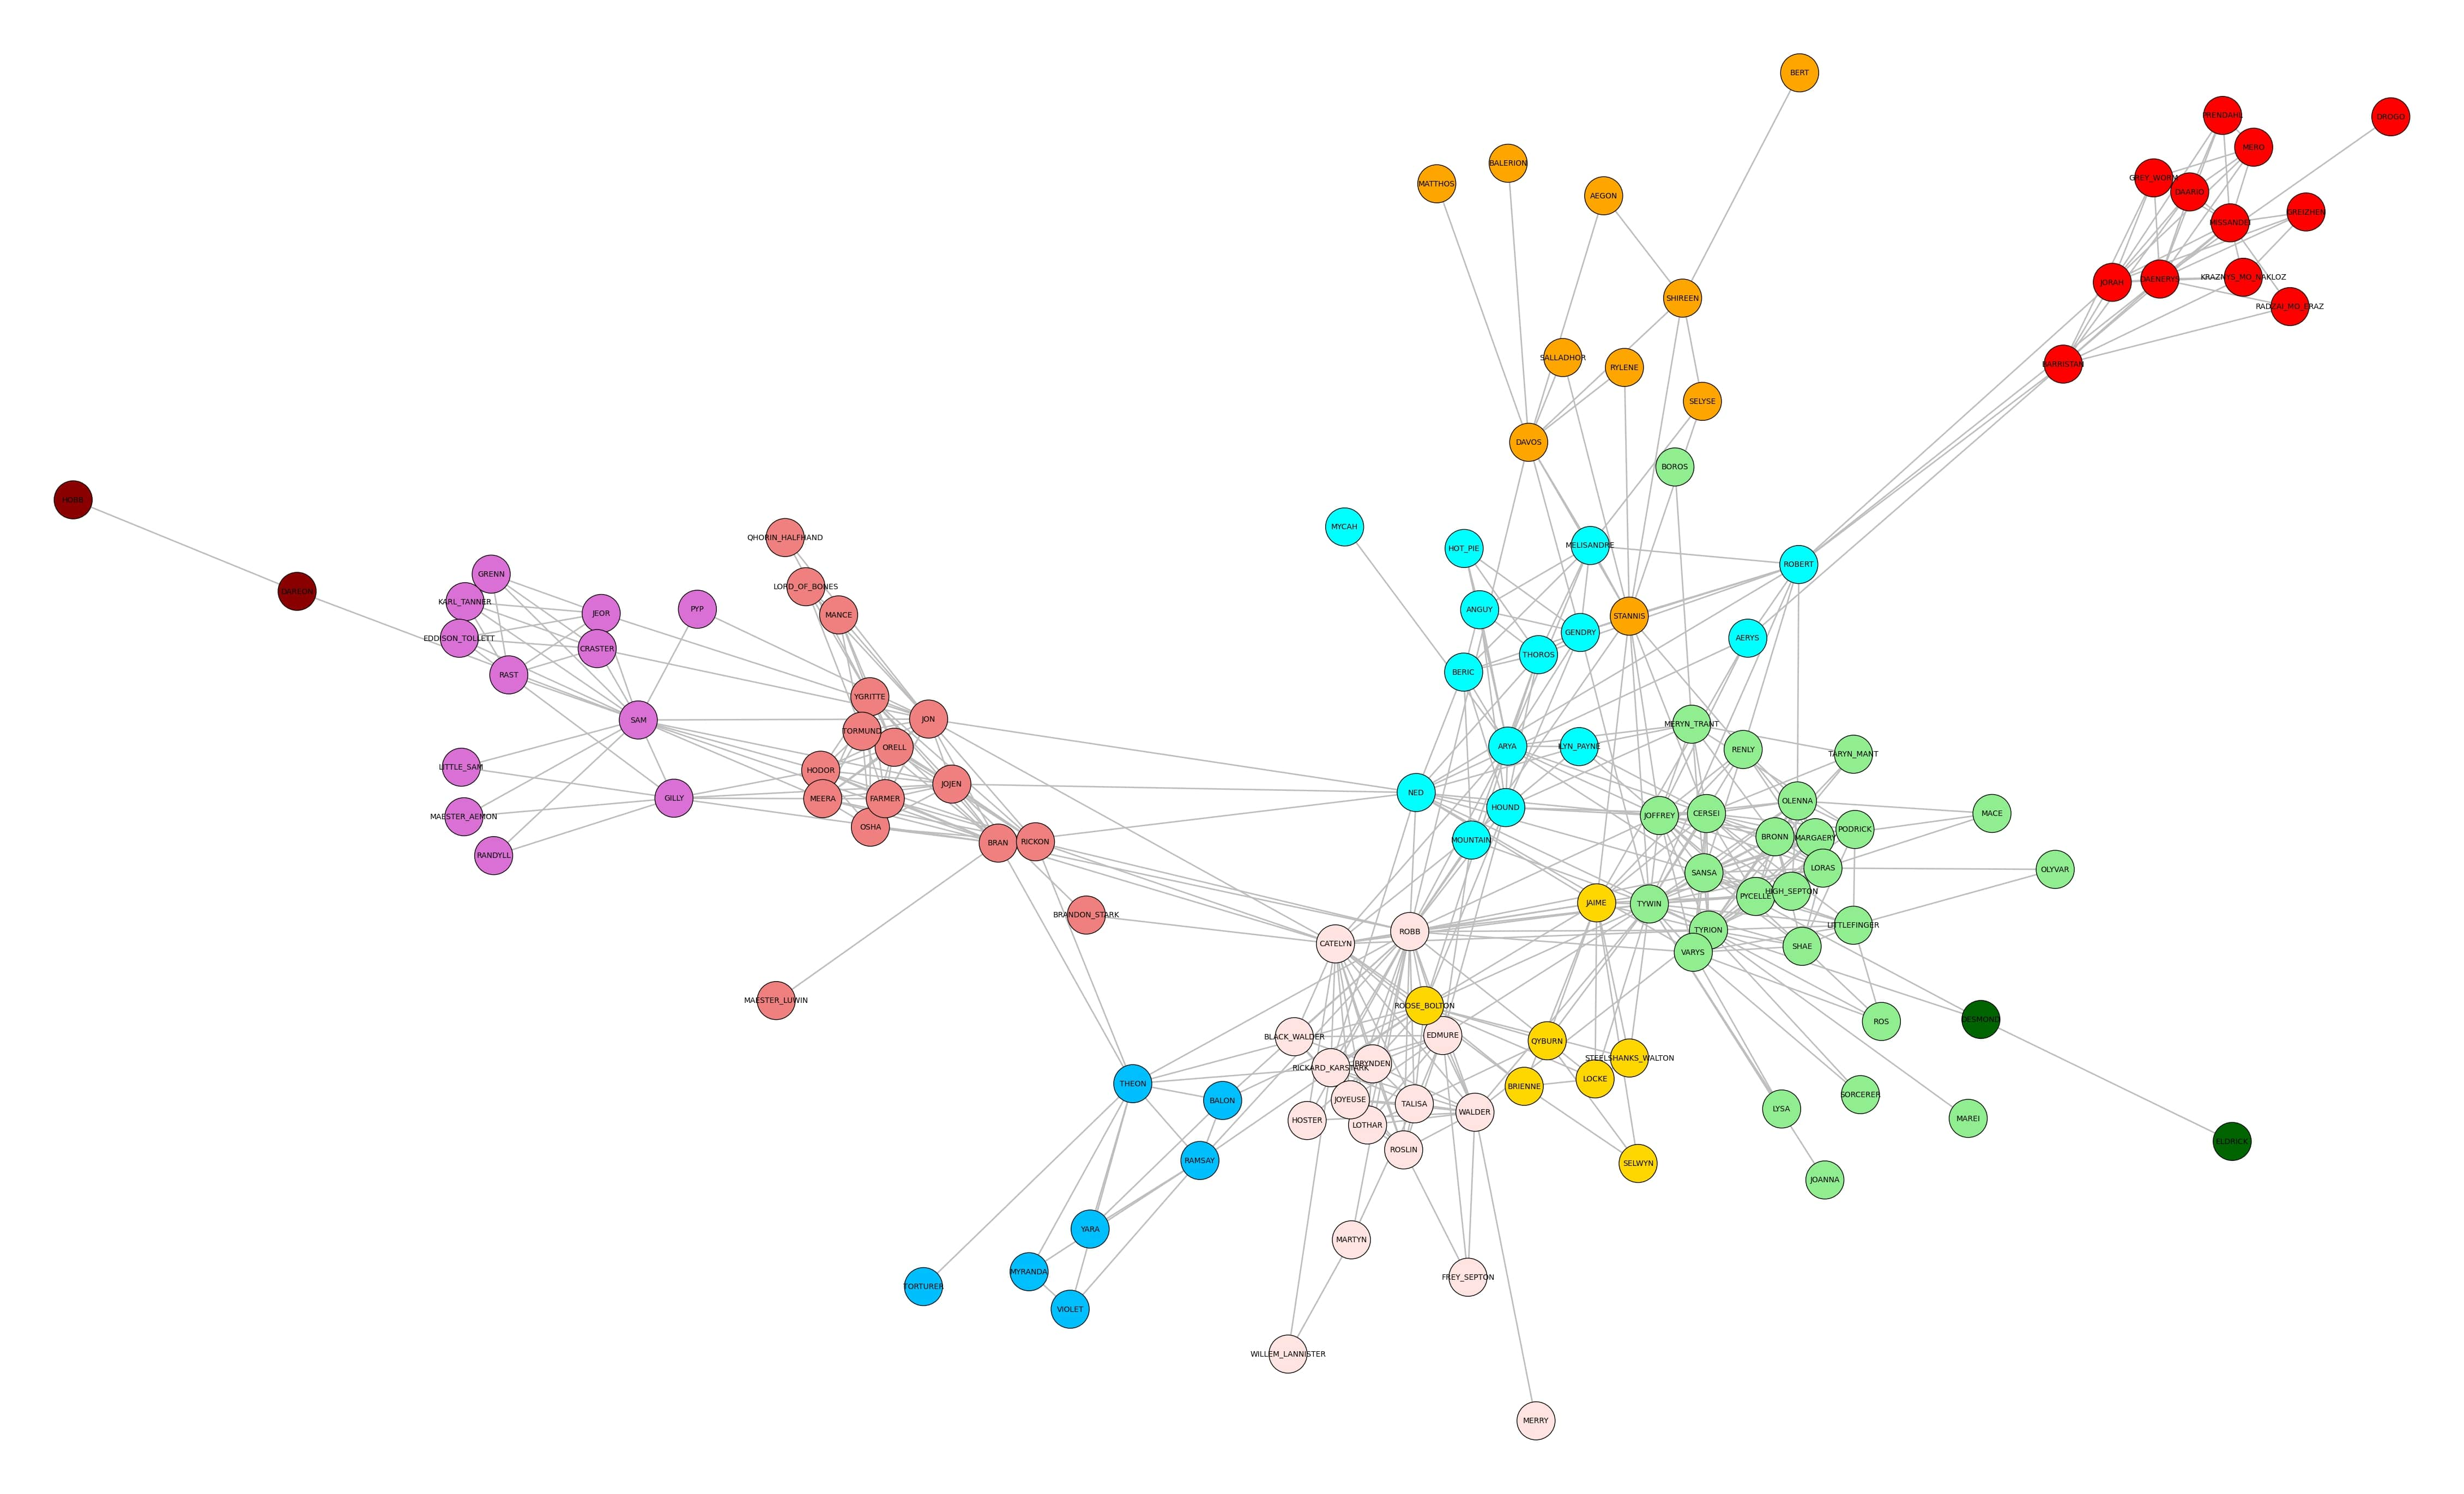
\includegraphics[width=0.4\textwidth]{img/s3/communities_infomap.jpg}
    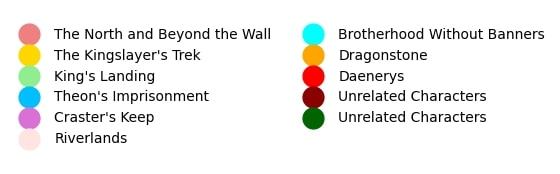
\includegraphics[width=0.4\textwidth]{img/s3/infomap_legend.jpg}\\
    \caption{\small{$\#communities=11$, $modularity=0.616$}}
    \label{fig:infomap_s3}
    \vspace{2.5cm}
\end{figure}

\begin{figure}[!h]
    \centering
    \textbf{Girvan-Newman} \\
    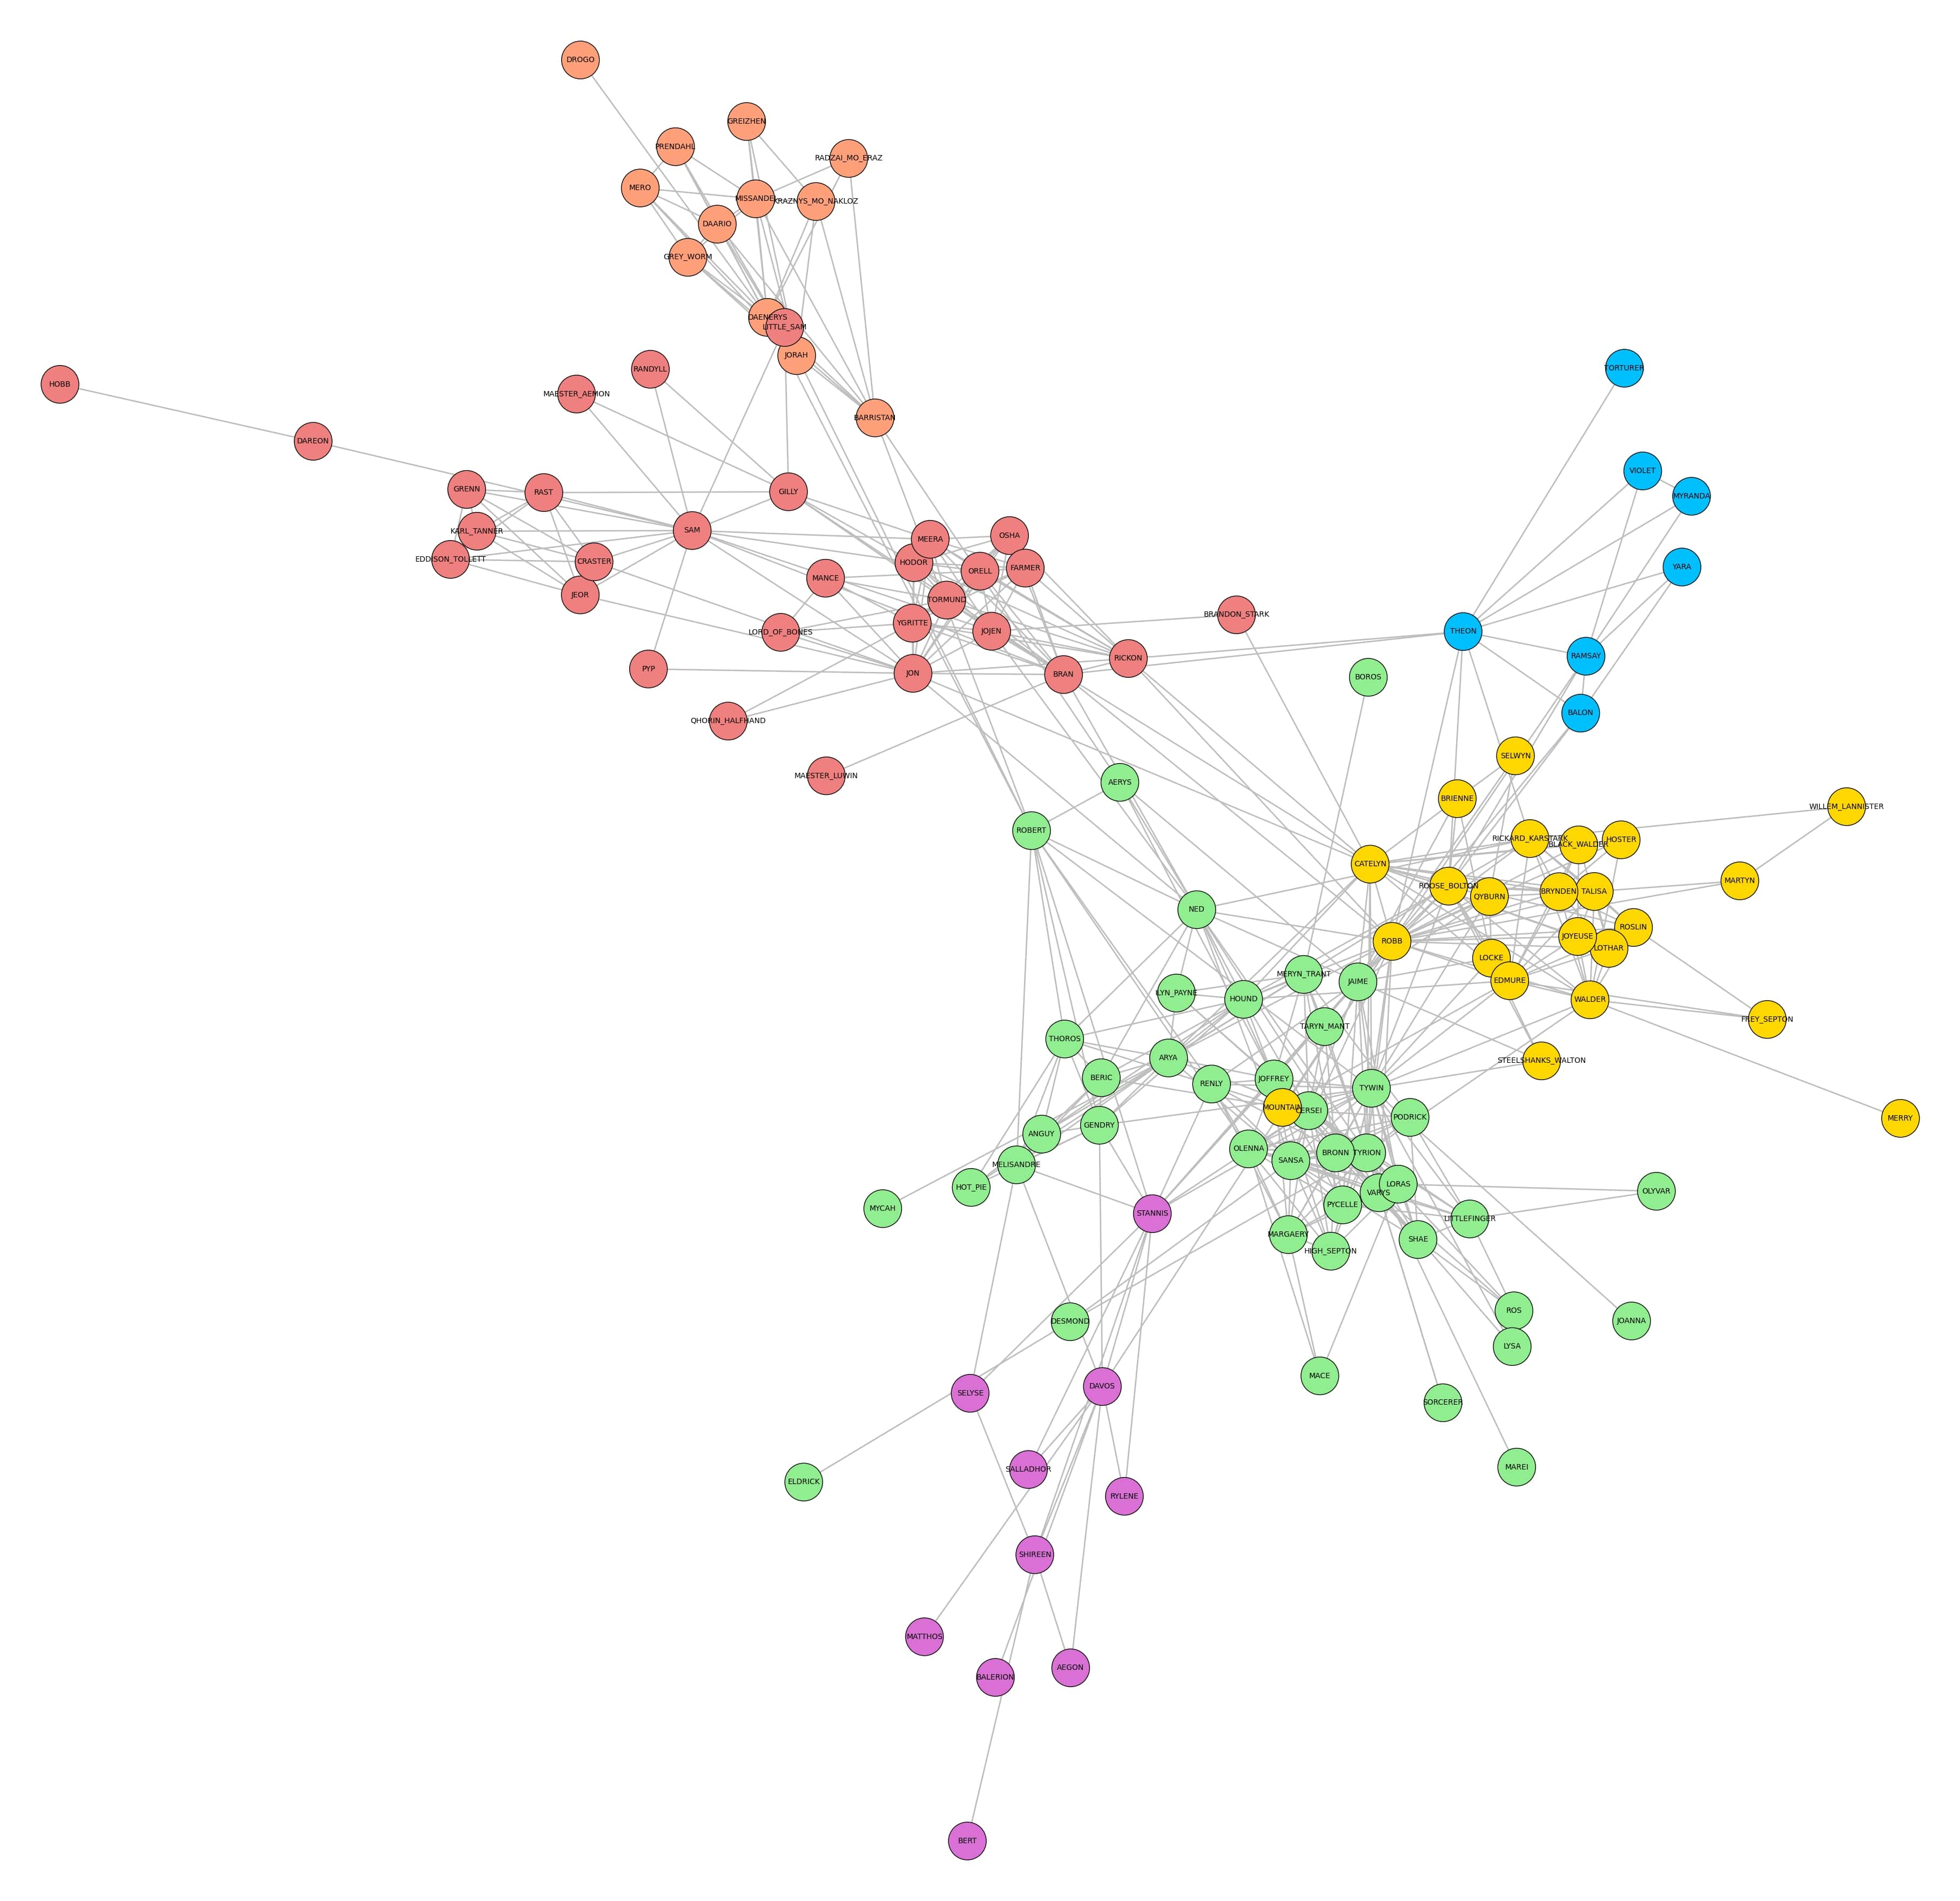
\includegraphics[width=0.4\textwidth]{img/s3/communities_g-n.jpg}
    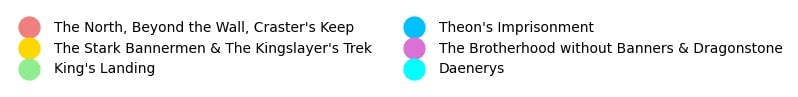
\includegraphics[width=0.5\textwidth]{img/s3/g-n_legend.jpg}\\
    \caption{\small{$\#communities=6$, $modularity=0.589$}}
    \label{fig:gn_s3}
    \vspace{2cm}
\end{figure}


\begin{figure}[!h]
    \centering
    \textbf{Louvain} \\
    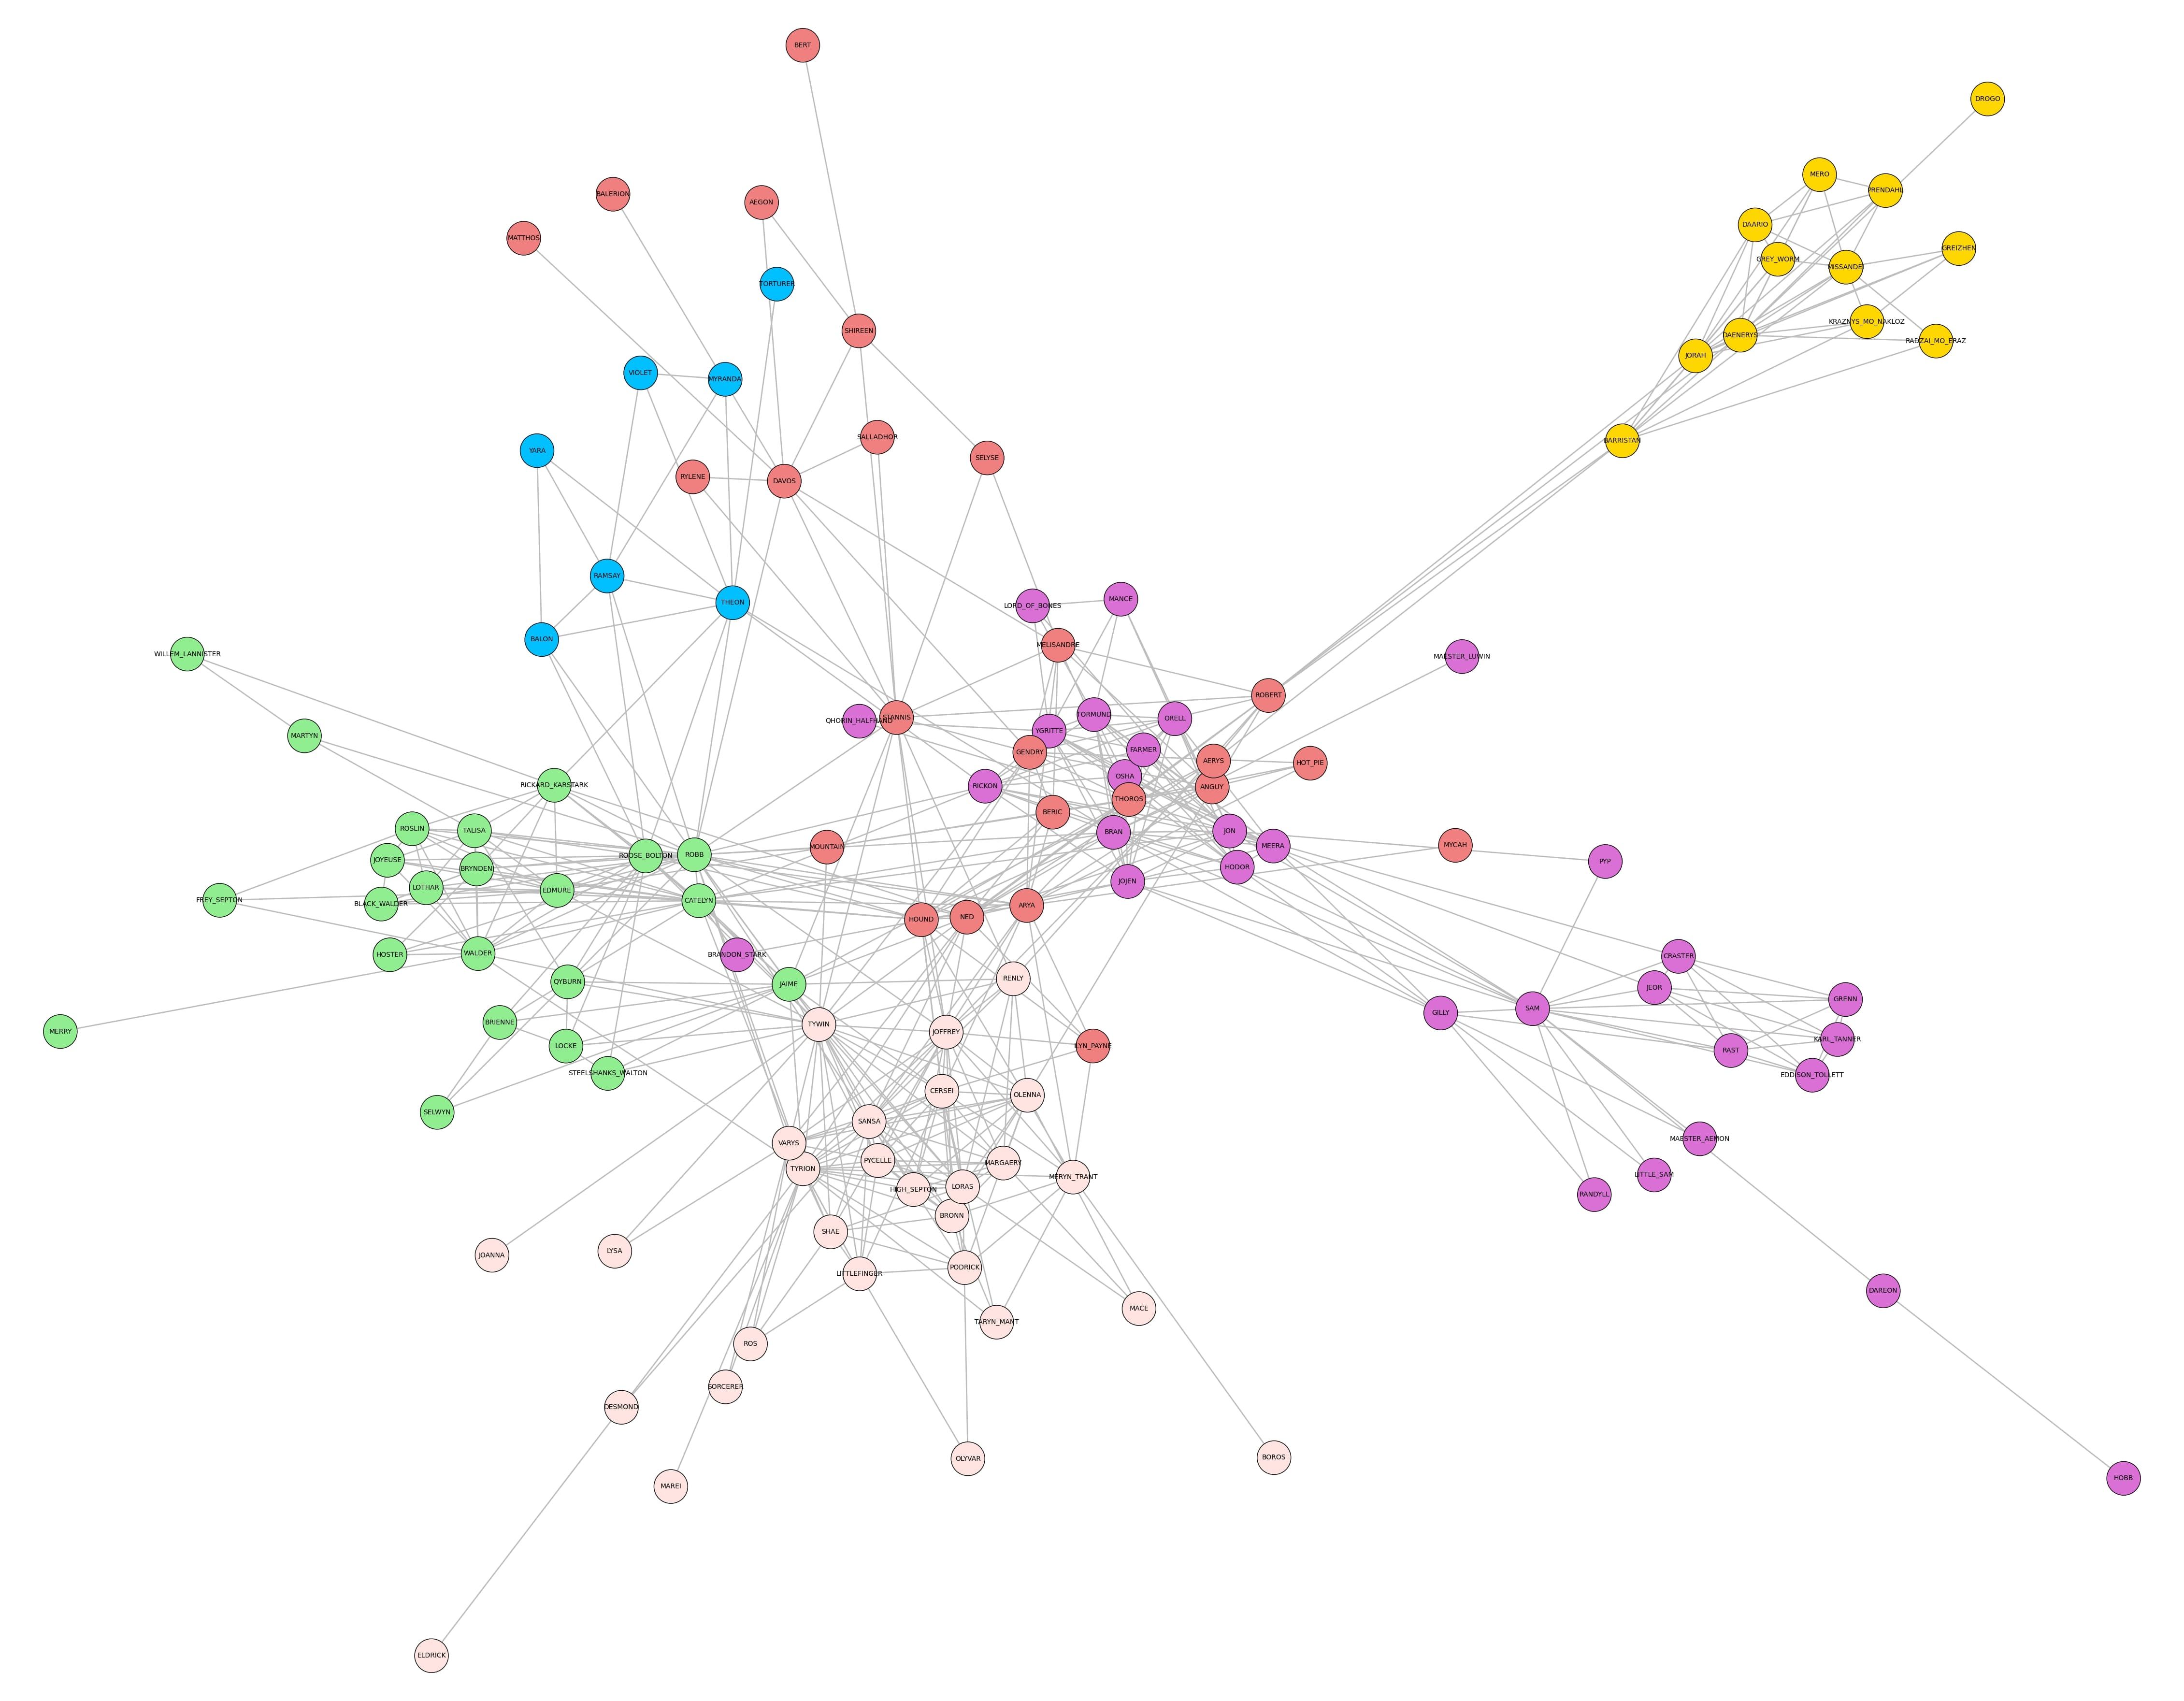
\includegraphics[width=0.5\textwidth]{img/s3/communities_louvain.jpg}
    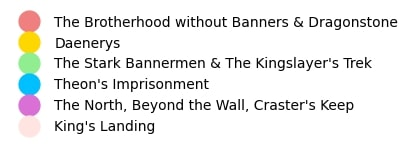
\includegraphics[width=0.3\textwidth]{img/s3/louvain_legend.jpg}\\
    \caption{\small{$\#communities=6$, $modularity=0.626$}}
    \label{fig:louvain_s3}
    \vspace{1cm}
\end{figure}



\begin{figure}[!h]
    \centering
    \textbf{Greedy Modularity Maximization}\\
    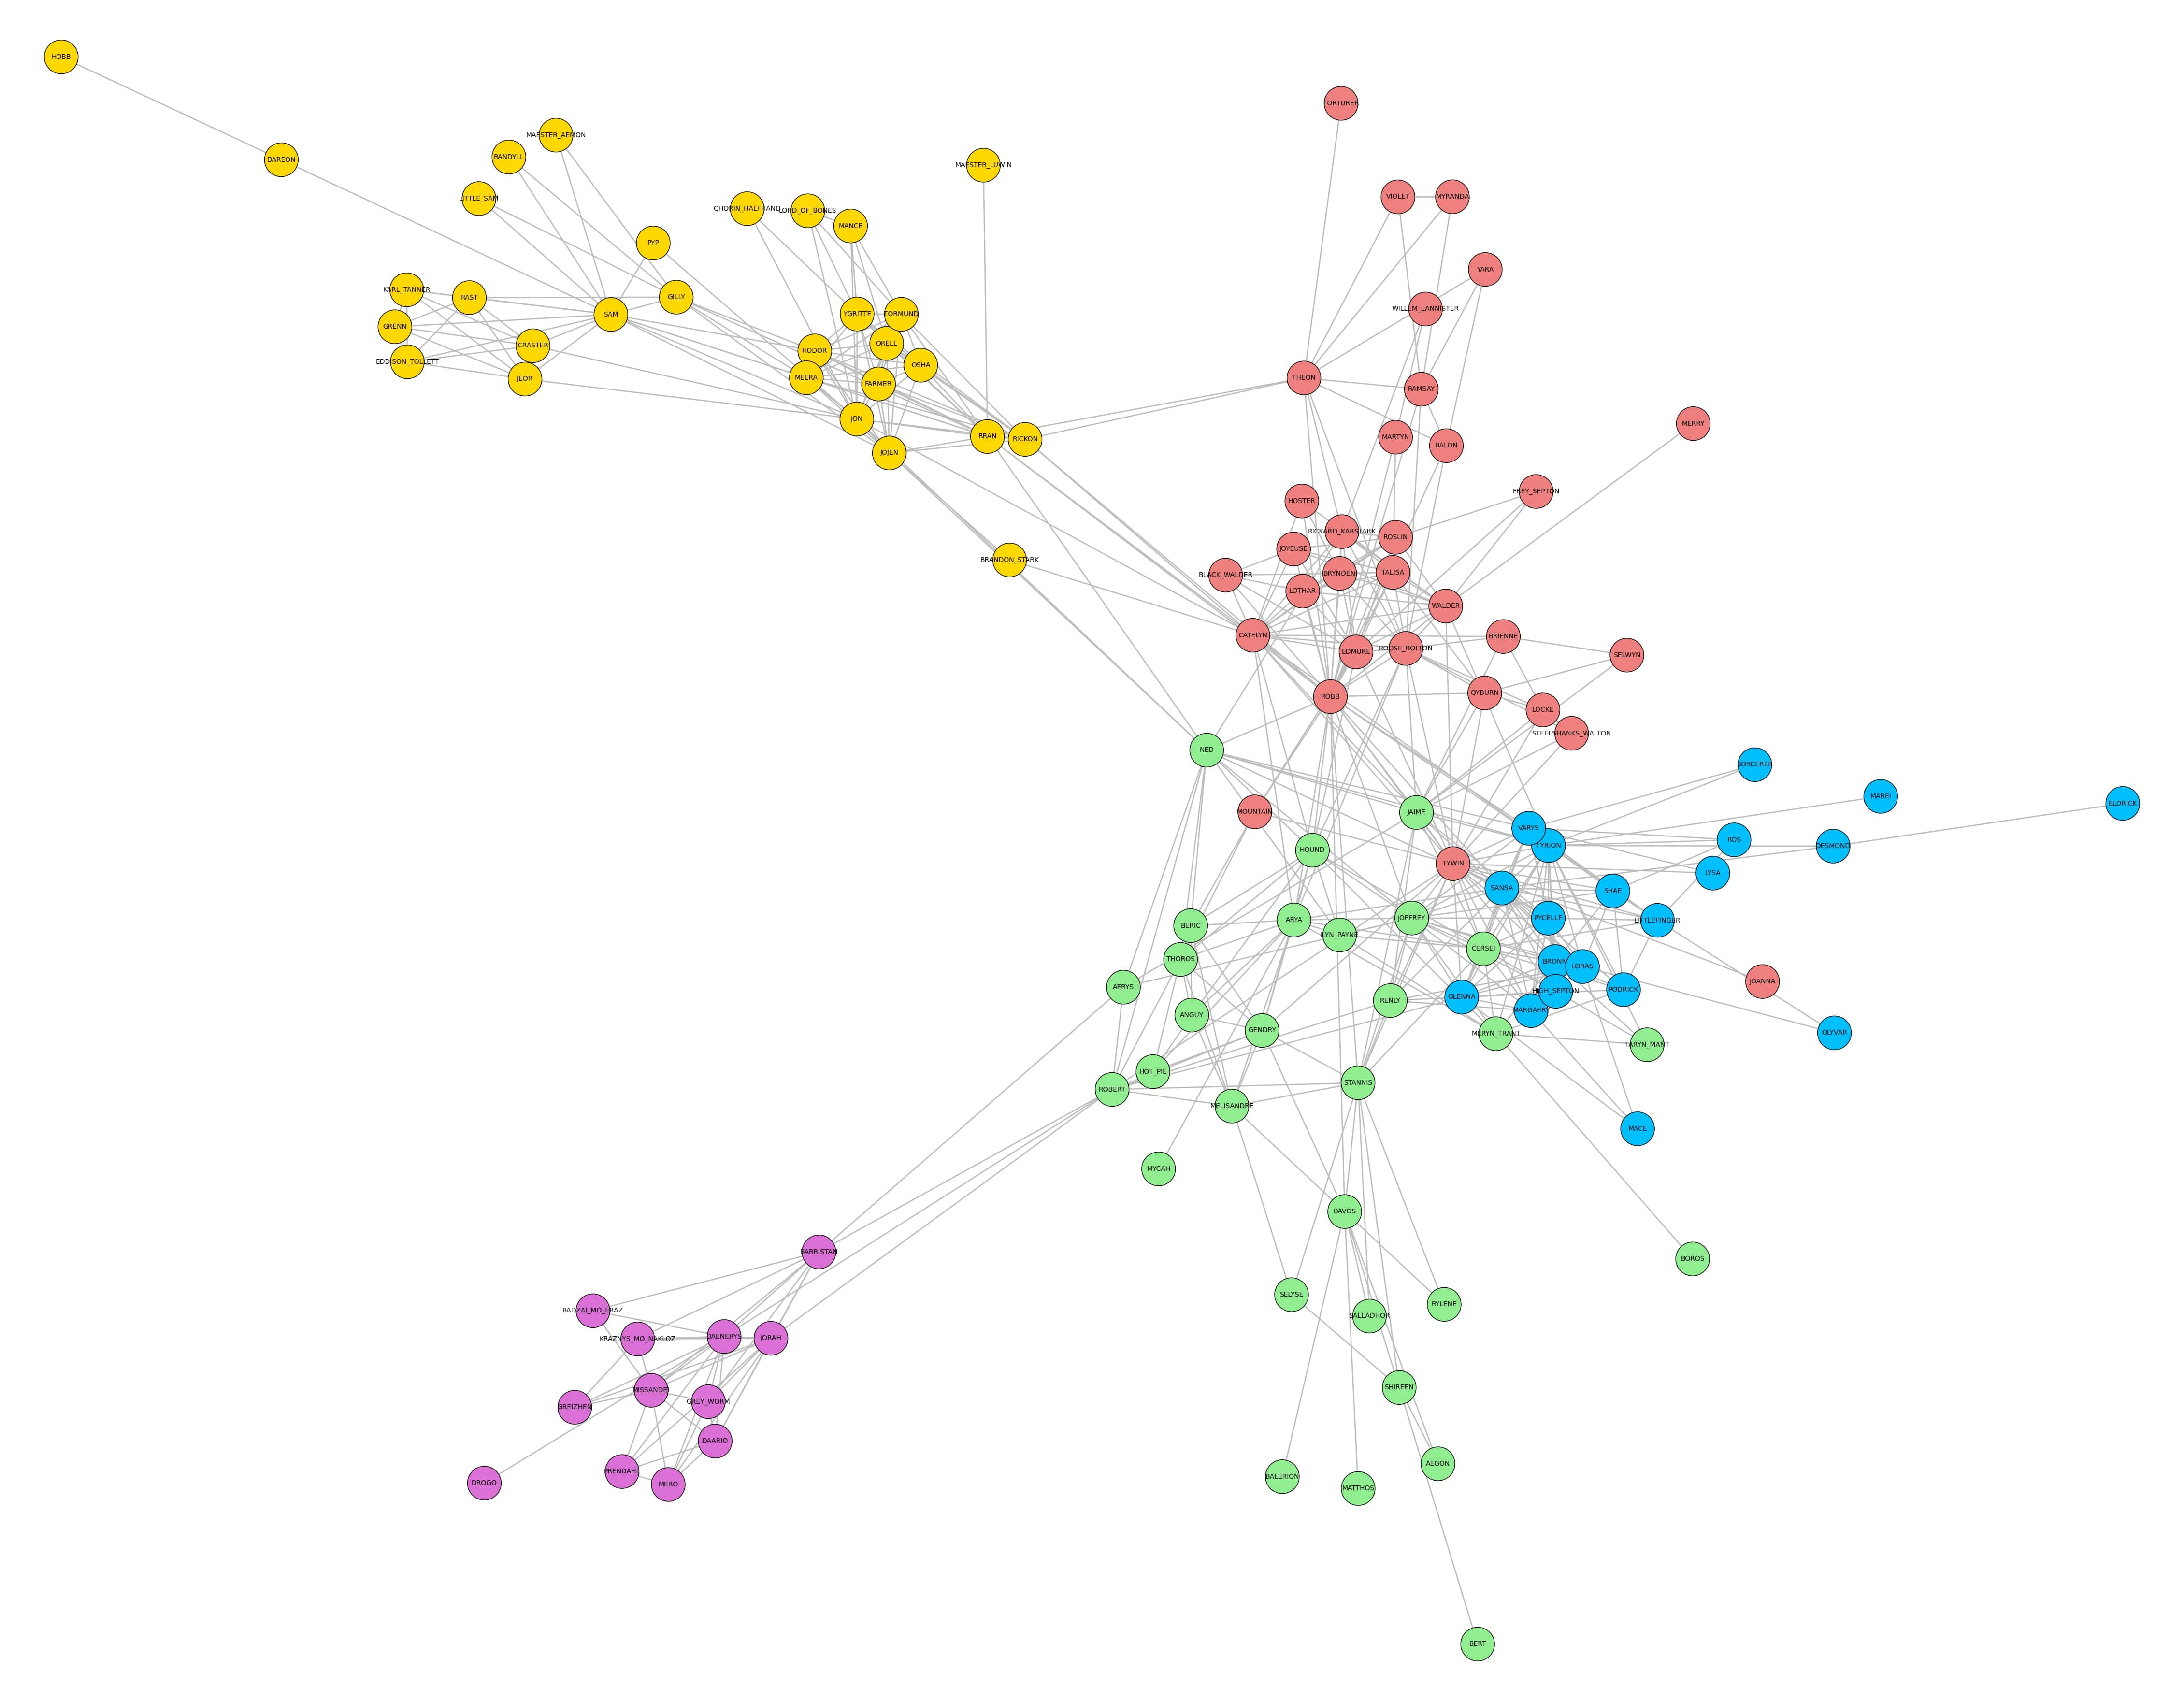
\includegraphics[width=0.5\textwidth]{img/s3/communities_gmm.jpg}
    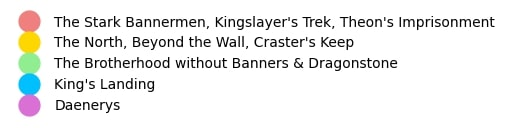
\includegraphics[width=0.4\textwidth]{img/s3/gmm_legend.jpg}\\
    \caption{\small{$\#communities=5$, $modularity=0.581$}}
    \label{fig:gmm_s3}
\end{figure}


\begin{figure}[!h]
    \centering
    \textbf{Spectral Clustering}
    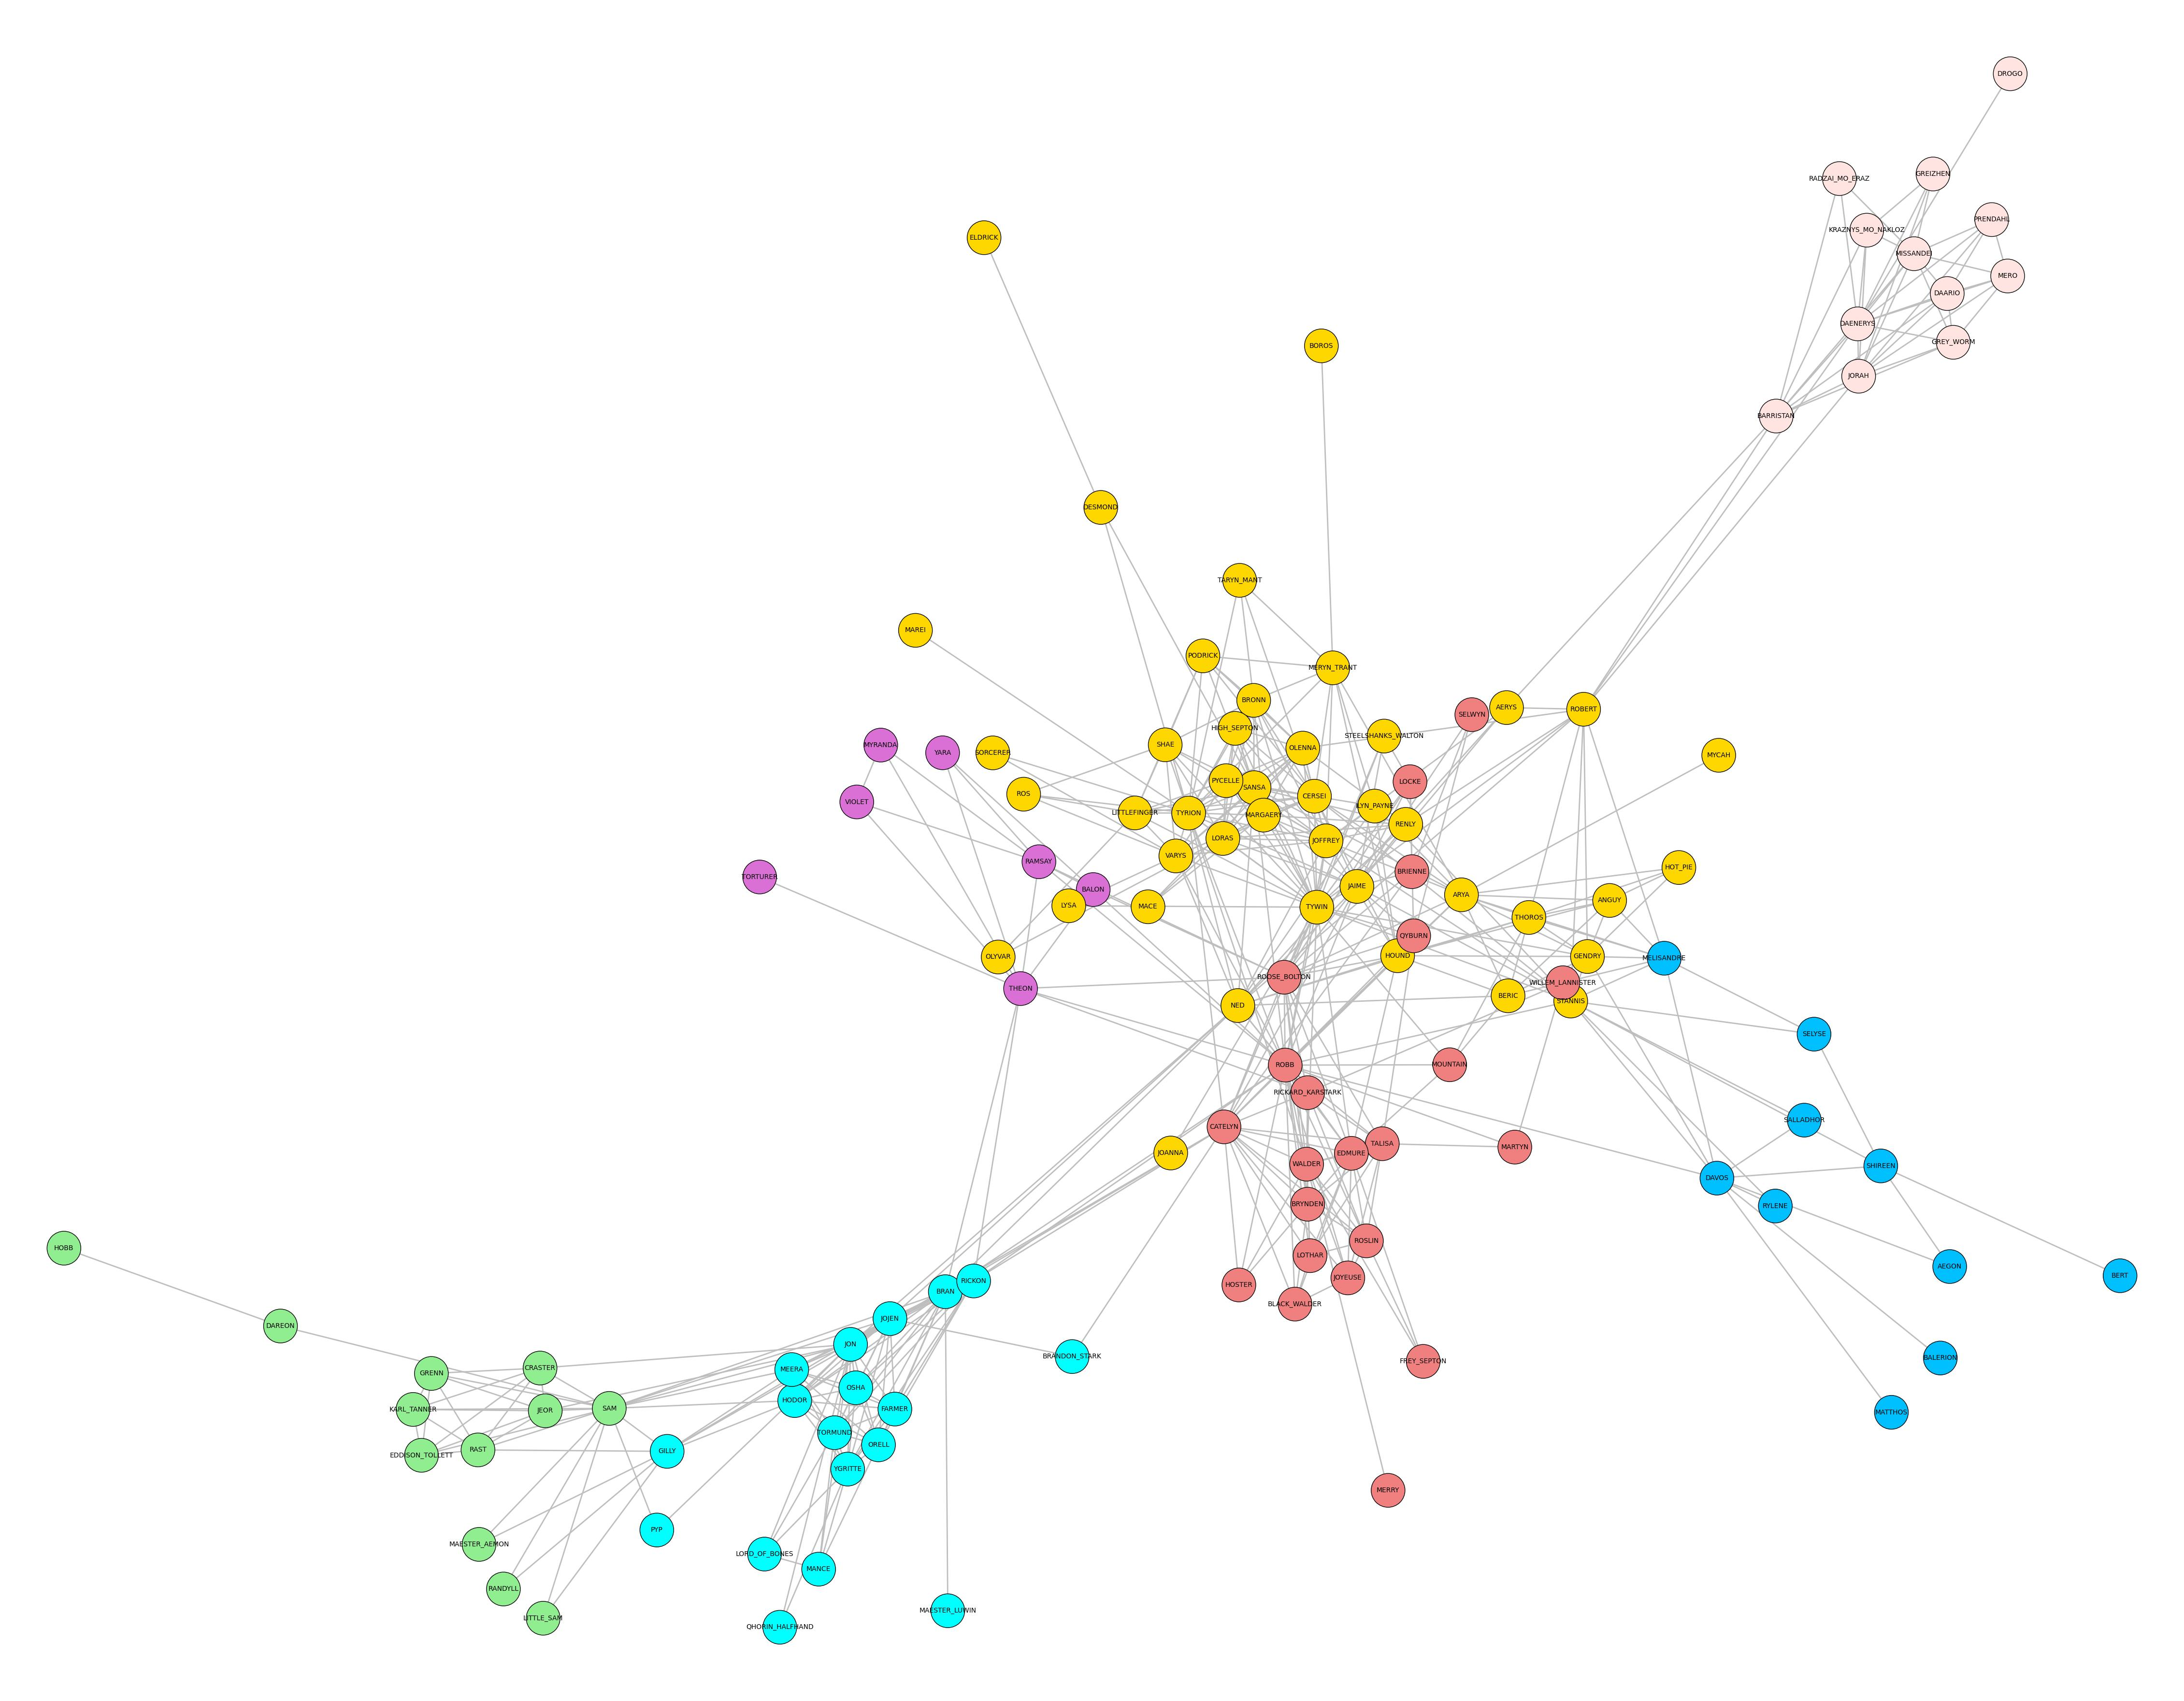
\includegraphics[width=0.5\textwidth]{img/s3/communities_sc.jpg}
    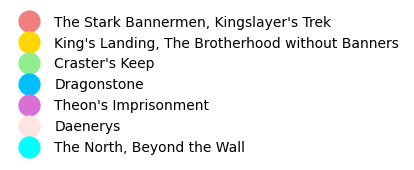
\includegraphics[width=0.3\textwidth]{img/s3/sc_legend.jpg}\\
    \caption{\small{$\#communities=7$, $modularity=0.576$}}
    \label{fig:sc_s3}
    \vspace{2cm}
\end{figure}



\paragraph{Comparison Between Methods}

Below, the various community detection methods are compared with respect to performance on Season 3's graph.

\begin{figure}[!h]
    \centering
    \includegraphics[width=0.5\textwidth]{img/s3/communities_comparison.jpg}
\end{figure}



\textbf{Infomap}\textsuperscript{\ref{fig:infomap_s3}} detects 11 communities, which roughly match the expected ones. The modularity score reached is 0.616. However, there are two communities of a couple of characters each which should realistically be part of the communities they are connected to but are characters so marginal that they are put in distinct clusters. Here, the communities of the Brotherhood without Banners and Dragonstone are considered by Infomap as two different communities, even if a lot of characters do have cross-interactions. It is worth noting how Ned and Robert appear in the network. They both died in the first season, yet they continue to play prominent roles as connectors. Both Ned and Robert are on the lips of people across the network. Ned appears in the Brotherhood without Banners community due to an extended discussion of the Lord of Winterfell between Arya, Beric and Thoros, as the latter two try to earn her trust. Robert’s blood is essential for Melisandre’s magic, pulling it into the same community. Also, Robert almost entirely holds Daenerys' community connected to the graph, unlike in Season 2, mostly by connecting Ser Barristan Selmy, who meets Daenerys during this season.

\textbf{Girvan-Newman}\textsuperscript{\ref{fig:gn_s3}} struggles to separate theoretical communities that are close together, but does a better job in this season. The modularity score is 0.589.

\textbf{Louvain}\textsuperscript{\ref{fig:louvain_s3}} detects 6 communities with a modularity of 0.626. The Brotherhood without Banners and Dragonstone are considered a single community, which is reasonable. Jaime and Brienne don't form the small community described above, that encompasses the return to King's Landing, rather they are all grouped together with the Stark Bannermen. Characters in the North are grouped together, so there is no distinction between the community beyond the Wall (Jon), and the one at Craster's Keep (Sam).

\textbf{Greedy Modularity Maximization}\textsuperscript{\ref{fig:gmm_s3}} method finds 5 communities, with a modularity of 0.581. The communities found are somewhat similar to the ones found by Louvain, with the exception that Theon's Imprisonment is grouped with the Stark's Bannermen. There is also an unexpected separation of Brienne and Jaime, where the latter is clustered into a community mixing King's Landing characters and ones from The Brotherhood without Banners and Dragonstone. Therefore, Greedy Modularity Maximization did not do a good job in distinguishing some communities.

\textbf{Spectral Clustering}\textsuperscript{\ref{fig:sc_s3}} detects 7 communities with a 0.576 modularity score. The Dragonstone community is separate from the Brotherhood without Banners. The Stark Bannermen and the Kingslayer's Trek communities are clustered together, which mostly makes sense since Jaime's and Brienne journey starts from Catelyn ordering Brienne to escort Jaime back to King's Landing.

Overall, Louvain scores the best in terms of modularity, although the clustering is not perfect. Infomap detected all the theoretical communities separately, although marginal characters in Craster's Keep and King's Landing are considered separate communities.

\subsubsection{Triangles}

Below are listed\textsuperscript{\ref{tab:tr_s3}} and visualized\textsuperscript{\ref{fig:tr_s3}}  the most interesting triangles

\begin{table}[h!]
    \centering
    \small
    \begin{tabular}{c|c|c}
        Triangle & Strength & Strongest Edge  \\
        \hline
        \small{(Jon, Ygritte, Tormund)} & 222 & 159 \small{(Jon, Ygritte)} \\
        \small{(Tyrion, Tywin, Sansa)} & 211 & 115 \small{(Tyrion, Tywin)}\\
        \small{(Brienne, Jaime, Locke)} & 201 & 127 \small{(Brienne, Jaime)}\\
        \small{(Tyrion, Tywin, Sansa)} & 211 & 115 \small{(Tyrion, Tywin)}\\
        \small{(Tyrion, Cersei, Joffrey)} & 176 & 95 \small{(Tyrion, Cersei)}\\
        \small{(Robb, Talisa, Catelyn)} & 174 & 89 \small{(Robb, Talisa)}\\
        \small{(Brienne, Jaime, Roose Bolton)} & 165 & 127 \small{(Brienne, Jaime)}\\
        \small{(Daenerys, Jorah, Barristan)} & 163 & 69 \small{(Daenerys, Jorah)}\\
        \small{(Arya, Hound, Thoros)} & 159 & 79 \small{(Arya, Hound)}\\
        \hline 
    \end{tabular} \\
    \vspace{0.2cm}
    \caption{Strength of interesting triangles}
    \label{tab:tr_s3}
\end{table}

\begin{figure}[!h]
    \centering
    \includegraphics[width=0.5\textwidth]{img/s3/interesting_triangles.jpg}
    \caption{\small{Interesting triangles in Season 3's graph}}
    \label{fig:tr_s3}
\end{figure}

Beyond the Wall, Jon and Ygritte fall in love ($weight_{j,y}=159$), as it is possible to see from the triangle formed between the two and Jon's new wildling friend Tormund ($weight_{j,t}=35$). 

Even though Sansa and Tyrion get married through an unwilling political marriage ($weight_{s,t}=85$), interactions between Tyrion and his father Tywin are constantly the strongest in triangles involving the two ($weight_{tyw,tyr}=115$). This is backed up from the story, as Tyrion is stripped of his position as Hand of the King. His father, Tywin Lannister, takes over the role, further straining their already tense relationship. Though, the relationship between Tyrion and Cersei is still strong and tense; Cersei, in fact, interacts more with him ($weight_{c,t}=95$) than with her own son Joffrey ($weight_{j,c}=54$). 

Jaime, known as the Kingslayer, gets escorted by Brienne of Tarth to King's Landing, and during their journey they strongly bond ($weight_{j,b}=127$), even when captured by Locke. 

The triangle between Robb, Talisa and Catelyn shows how much Robb loves his new bride Talisa ($weight_{r,t}=89$), even compared to the interactions he has with his mother Catelyn. 

Danenerys has two advisors, Jorah, and the newly arrived Barristan ($weight_{d,b}=37$). Though, she is, as always, closer to Jorah ($weight_{d,j}=69$).

When leaving the Brotherhood without Banners, Arya is captured by Sandor Clegane, who intends to ransom her to her family at Riverrun. Arya and the Hound share a complex relationship. Despite her initial hatred for him, Arya begins to understand the Hound's pragmatic and brutal outlook on life. Their strong interactions are filled with tension, dark humor, and mutual learning ($weight_{s,a}=79$).



\subsubsection{Link Prediction}

\paragraph{Preferential Attachment}

Jamie is Cersei's twin brother and lover. The two are deeply bound to each other in a toxic and destructive love. Jamie, having been captured by Robb's forces, is clearly in the center of a possible strong triangle between Robb and Cersei. Link prediction through preferential attachment predicts Cersei and Robb to be the most likely to have a link, with a score of 620.

\newpage

\subsection{Season 4}

\begin{figure}[!h]
    \centering
    \includegraphics[width=0.48\textwidth]{img/s4/frames_s4.jpg}
\end{figure}

\begin{table}[!h]
    \centering
    \small
    \begin{tabular}{c|c}
        Description & Value  \\
        \hline
        Nodes & 169\\
        Edges & 664 \\
        Graph Density & 0.046 \\
        Connected Graph & Yes \\
        Number of Components & 1 \\
        Small-World Network & Yes ($\lambda=1.29$ , $\gamma=18.03$) \\
        Diameter & 8 \\
        Avg. Shortest Path & 3.47 \\
        Avg. Degree & 7.86 [1,40] \\
        Most Freq. Degree & 2 \\
        Number of Bridges & 15 \\
        Deg. Assortativity Coeff. & -0.082\\
        Global Clustering Coeff. & 0.435 \\
        Average Clustering Coeff. & 0.667 \\
        \hline 
    \end{tabular}
    \vspace{0.2cm}
    \caption{Summary table for Season 4's network}
    \label{tab:my_label}
\end{table} 

\begin{figure}[!h]
    \centering
    \includegraphics[width=0.5\textwidth]{img/s4/degree_plot.jpg}
    \caption{\small{Degree distribution of Season 4}}
\end{figure}


\subsubsection{Centrality}

Below, the plot of Season 4's graph is presented. Node sizes are scaled according to PageRank centrality, and the layout is computed using the Fruchterman-Reingold force-directed layout algorithm.


\begin{figure}[!h]
    \centering
    \includegraphics[width=0.3\textwidth]{img/s4/pagerank_graph.jpg}
\end{figure}


The following table reports the results obtained by the different centrality measure.

\begin{table}[!h]
    \centering
    \small
    \begin{tabular}{c|c|c}
        Measure & Character & \small{Highest Centrality Score} \\
        \hline
                    & Joffrey & 0.212 \\
                    & Ned & 0.201 \\
        Betweenness & Stannis & 0.184 \\
                    & Jon & 0.151 \\
                    & Varys & 0.112 \\
        \hline 
                    & Joffrey & 0.460 \\
                    & Jaime & 0.435 \\
        Closeness   & Ned & 0.427 \\
                    & Cersei & 0.417 \\
                    & Tyrion & 0.414 \\
        \hline 
                    & Joffrey & 0.294 \\
                    & Tyrion & 0.288 \\
        Eigenvector & Cersei & 0.270 \\
                    & Jaime & 0.254 \\
                    & Sansa & 0.259 \\
        \hline 
                    & Joffrey & 0.011 \\
                    & Tyrion & 0.012 \\
        Harmonic    & Cersei & 0.012 \\
                    & Sansa & 0.012 \\
                    & Jon & 0.012 \\
        \hline
                    & Joffrey & 0.238 \\
                    & Tyrion & 0.226 \\
        Degree      & Cersei & 0.196 \\
                    & Sansa & 0.185 \\
                    & Jon & 0.179 \\
        \hline
                    & Tyrion & 1.000 \\
                    & Joffrey & 0.707 \\
        Weighted Degree & Jaime & 0.683 \\
                    & Cersei & 0.669 \\
                    & Sansa & 0.619 \\
        \hline
                    & Joffrey & 0.025 \\
                    & Tyrion & 0.024 \\
        PageRank    & Cersei & 0.020 \\
                    & Arya & 0.020 \\
                    & Sansa & 0.019 \\
        \hline
    \end{tabular}
    \vspace{0.2cm}
    \caption{Top characters with highest centrality scores}
    \label{tab:my_label}
\end{table}


\begin{table}[!h]
    \centering
    \begin{tabular}{c|c}
        Centrality Measure & Mean  \\
        \hline
        Betweenness & 0.013 \\
        Closeness & 0.389 \\
        Eigenvector & 0.059 \\
        Harmonic & 0.018 \\
        Degree & 0.069 \\
        Weighted Degree & 0.148 \\
        PageRank & 0.008 \\
        \hline 
    \end{tabular} \\
    \caption{Centrality means}
    \label{tab:my_label}
\end{table}


Tyrion's involvement in significant events, including Joffrey's death and his own trial, keeps him at the heart of the narrative. Tyrion's prominent centrality highlights his crucial role once again, particularly in the context of his trial and then his escape. His high Eigenvector and Weighted Degree Centrality scores show his widespread connections and the influence he has, despite being imprisoned for much of the season. Cersei's high centrality scores reflect her manipulative role in King's Landing politics, particularly in the aftermath of Joffrey's death.

\subsubsection{Communities}

In season 4, it is possible to find 8 main communities:

\begin{itemize}
    \item \textbf{The Riverlands}: Arya Stark and Sandor "The Hound" Clegane travel together across the Riverlands for much of the season ($weight_{a,s}=162$). The Hound plans to ransom Arya to her aunt Lysa Arryn in the Vale, but their journey takes a different turn. They meet the Lannister soldiers, the Riverrun soldiers, and Brienne of Tarth. Brienne, fights against the Hound over Arya's safety ($weight_{b,h}=22$). She defeats him, but Arya refuses to go with her and instead leaves the Hound to die, taking his money and heading towards Braavos. The events in this community significantly build up Arya's character arc.
    \item \textbf{King's Landing}: King Joffrey Baratheon marries Margaery Tyrell in a grand ceremony ($weight_{a,s}=36$). During the wedding feast, Joffrey is poisoned and dies in front of the entire court. Cersei accuses Tyrion of murdering the king ($weight_{c,t}=43$), and he is arrested and put on trial. The trial is biased against him, with several false witnesses, including Shae, Tyrion's former lover, testifying against him. Tyrion demands a trial by combat to determine his fate, but loses. Tyrion is freed from his cell by Jaime Lannister with the help of Varys. Before escaping, Tyrion seeks out his father, Tywin Lannister. Tyrion confronts Tywin about his betrayal and his treatment of him, eventually killing Tywin with a crossbow ($weight_{tyr,tyw}=94$). He then escapes King's Landing. With Joffrey's death, the power struggle between Cersei Lannister and Margaery Tyrell intensifies. The tensions between the Lannisters, Tyrells and Martells are quite evident by the clique\textsuperscript{\ref{fig:clique_s4}} of 8 characters in this community, involving Tyrion, Cersei, Jaime, Tywin, Joffrey, Tommen, Margaery, Mace and Oberyn.
    \item \textbf{The Eyrie}: After escaping King’s Landing following King Joffrey’s assassination at the Purple Wedding, Sansa is taken to the Vale by Littlefinger, and under his protection they arrive at the Eyrie, where they are welcomed by Lysa Arryn, Sansa’s aunt and the Lady of the Eyrie. There, Littlefinger manipulates the power dynamics and kills Lysa, effectively assuming control over the Vale. Sansa becomes more involved in Littlefinger’s schemes ($weight_{s,l}=96$), realizing that her survival depends on playing along with his plans.
    \item \textbf{Daenerys in Meereen}: Daenerys is carving a path through Slaver's Bay - not of conquest but of liberation. As functionally once a slave herself, Daenerys is determined to free the oppressed slaves of the region. First Astapor and then Yunkai fall before Daenerys's forces, and hundreds of thousands of freed slaves join to her banner. Yet Daenerys must now face the last and greatest of the slaver-cities, Meereen.
    \item \textbf{Castle Black and Mole's Town}: Jon is currently in Castle Black, and deals with situations arose by the developing friendship with Grenn and Edd ($weight_{j,g}=52$, $weight_{j,e}=42$), and the hathred-filled rivalry with Alliser ($weight_{j,a}=68$)and Janos ($weight_{jo,ja}=39$). In the meantime, Sam and Gilly are in Mole's Town.
    \item \textbf{Dragonstone}: Stannis is defeated at the Battle of the Blackwater and tries to rebuild his army. Then, Stannis and his newly acquired army arrive at the Wall just in time to intervene in the conflict between the Night's Watch and the wildlings led by Mance Rayder, who is then captured by Stannis.
    \item \textbf{Theon's Imprisonment}: Theon, now broken and tortured by Ramsay Bolton, is kept at the Dreadfort, another Bolton stronghold. Ramsay continues to torment Theon ($weight_{t,r}=63$), who has been psychologically and physically broken, adopting the identity of "Reek."
    \item \textbf{Beyond the Wall}: Bran's journey becomes mystical, as he continues to seek out the Three-Eyed Raven ($weight_{b,ter}=9$), a mysterious and ancient figure who has been guiding him through his visions. Bran ultimately meets him when is led into the cave beneath the weirwood tree.
    
\end{itemize}

\begin{figure}[!h]
    \centering
    \includegraphics[width=0.45\textwidth]{img/s4/clique.jpg} \\
    \caption{\small{Tyrion, Cersei, Jaime, Tywin, Joffrey, Tommen, Margaery, Mace and Oberyn form a clique that shows the strong tensions between Lannisters, Tyrells and Martells.}}
    \label{fig:clique_s4}
\end{figure}


\begin{figure}[!h]
    \centering
    \textbf{Infomap}  \\
    \includegraphics[width=0.35\textwidth]{img/s4/communities_infomap.jpg}
    \includegraphics[width=0.3\textwidth]{img/s4/infomap_legend.jpg}\\
    \caption{\small{$\#communities=11$, $modularity=0.6$}}
    \label{fig:infomap_s4}
\end{figure}


\begin{figure}[!h]
    \centering
    \textbf{Girvan-Newman} \\
    \includegraphics[width=0.35\textwidth]{img/s4/communities_g-n.jpg}
    \includegraphics[width=0.3\textwidth]{img/s4/g-n_legend.jpg}\\
    \caption{\small{$\#communities=5$, $modularity=0.573$}}
    \label{fig:gn_s4}
\end{figure}


\begin{figure}[!h]
    \centering
    \textbf{Louvain} \\
    \includegraphics[width=0.35\textwidth]{img/s4/communities_louvain.jpg}
    \includegraphics[width=0.35\textwidth]{img/s4/louvain_legend.jpg}\\
    \caption{\small{$\#communities=7$, $modularity=0.6$}}
    \label{fig:louvain_s4}
\end{figure}



\begin{figure}[!h]
    \centering
    \textbf{Greedy Modularity Maximization}\\
    \includegraphics[width=0.4\textwidth]{img/s4/communities_gmm.jpg}
    \includegraphics[width=0.4\textwidth]{img/s4/gmm_legend.jpg}\\
    \caption{\small{$\#communities=4$, $modularity=0.514$}}
    \label{fig:gmm_s4}
\end{figure}

\begin{figure}[!h]
    \centering
    \textbf{Spectral Clustering}
    \includegraphics[width=0.4\textwidth]{img/s4/communities_sc.jpg}
    \includegraphics[width=0.45\textwidth]{img/s4/sc_legend.jpg}\\
    \caption{\small{$\#communities=8$, $modularity=0.581$}}
    \label{fig:sc_s4}
    \vspace{6cm}
\end{figure}

\newpage

\paragraph{Comparison Between Methods}

Below, the various community detection methods are compared with respect to performance on Season 4's graph.

\begin{figure}[!h]
    \centering
    \includegraphics[width=0.5\textwidth]{img/s4/communities_comparison.jpg}
\end{figure}

\textbf{Infomap}\textsuperscript{\ref{fig:infomap_s4}} detects 11 communities with a modularity of 0.6. Besides the fact that the Dragonstone community is not well detected and clustered with another one, it is clear that in this case four of the communities should be part of the main ones; indeed, Infomap fails to recognize marginal characters as part of their actual community. For example, there is no reason why the three slaves in the red community should not be in Daenerys' commmunity. 

\textbf{Girvan-Newmann}\textsuperscript{\ref{fig:gn_s4}} detects 5 communities, with a modularity of 0.573. Trying to further find other communities does not yield any better results, as those would be composed of single characters. Although there are no insignificant communities, the Eyrie community is inside the King's Landing one, and all communities towards Dragonstone and the far north of Westeros are clustered into one.

\textbf{Louvain}\textsuperscript{\ref{fig:louvain_s4}} finds 7 communties, with a modularity of 0.6. Dragonstone is, as before, grouped with Jon's and Sam's community. Otherwise, the communities are correctly formed. 

\textbf{Greedy Modularity Maximization}\textsuperscript{\ref{fig:gmm_s4}} does not perform well on Season 4's graph. Indeed, it finds 4 communities, with a modularity of 0.514. Only three of these are significant, but the red and yellow communities cluster together most of the actual communities.

\textbf{Spectral Clustering}\textsuperscript{\ref{fig:sc_s4}} detects 7 communities, though two of them are not significant and the red and yellow ones are composed of two or more real communities. The modularity score is 0.581.

Overall, Infomap and Louvain yield the highest modularity score, both 0.6. In particular, if we discard Infomap's insignificant communities, this method perform the best. Louvain, on the other hand, is more conservative and, although it finds the correct communities, two of them are clustered together. The worst method is Greedy Modularity Maximization, which fails to distinguish communities which are not very clearly separated.

\subsubsection{Triangles}

The following table lists the most interesting triangles, which are visualized in the graph below.

\begin{table}[h!]
    \centering
    \small
    \begin{tabular}{c|c|c}
        Triangle & Strength & Strongest Edge  \\
        \hline
        (Arya, Hound, Brienne) & 220 & 162 (Arya, Hound) \\
        (Jaime, Tyrion, Tywin) & 324 & 147 (Jaime, Tyrion) \\
        (Jaime, Tyrion, Cersei) & 321 & 147 (Jaime, Tyrion) \\
        (Tyrion, Cersei, Joffrey) & 150 & 64 (Tyrion, Joffrey) \\
        (Cersei, Joffrey, Margaery) & 117 & 43 (Cersei, Margaery) \\
        (Littlefinger, Sansa, Lysa) & 239 & 96 (Littlefinger, Sansa) \\
        (Daenerys, Jorah, Missandei) & 180 & 106 (Daenerys, Jorah) \\
        \hline 
    \end{tabular} \\
    \vspace{0.2cm}
    \caption{Strength of interesting triangles}
    \label{tab:my_label}
\end{table}

\begin{figure}[!h]
    \centering
    \includegraphics[width=0.4\textwidth]{img/s4/s4_triangles.jpg}
    \caption{\small{Interesting triangles in Season 4}}
\end{figure}

As stated before, The Hound and Brienne of Tarth fight over Arya's protection. Though, the interaction is quite brief, compared to the strong bond that Arya and The Hound share. Jamie is very close to Tyrion ($weight_{t,j}=147$), and helps him escape King's Landing, closer than he is with Cersei. It is interesting to note that, although Cersei is Joffrey's mother, Tyrion has a stronger edge with him, probably due to the fact that he is accused of Joffrey's murder. Moreover, it is noteworthy that there is a lot of tension between Cersei and Margaery.
Meanwhile in the Eyrie, Littlefinger and Sansa share the strongest edge in the triangle involving him, Sansa and Lysa. The latter is deeply obsessed with Littlefinger, but in turn, he has a strong romantic interest in Sansa. Finally, Daenerys bonds with a former Meereen slave, Missandei. Daenerys' bond with Jorah remain apparently strong, but during the season she finds out about Jorah's previous betrayal and exiles him. 




\subsection{Season 5}

\begin{figure}[!h]
    \centering
    \includegraphics[width=0.5\textwidth]{img/s5/s5_frames.jpg}
\end{figure}


\begin{table}[!h]
    \centering
    \small
    \begin{tabular}{c|c}
        Description & Value  \\
        \hline
        Nodes & 118\\
        Edges & 395 \\
        Graph Density & 0.057 \\
        Connected Graph & Yes \\
        Number of Components & 1 \\
        Small-World Network & Yes ($\lambda=1.24$ , $\gamma=9.41$) \\
        Diameter & 8 \\
        Avg. Shortest Path & 3.216 \\
        Avg. Degree & 6.70 [1,40] \\
        Most Freq. Degree & 2 \\
        Number of Bridges & 18 \\
        Deg. Assortativity Coeff. & -0.198\\
        Global Clustering Coeff. & 0.407 \\
        Average Clustering Coeff. & 0.58 \\
        \hline 
    \end{tabular}
    \vspace{0.2cm}
    \caption{Summary table for Season 5's network}
    \label{tab:my_label}
\end{table} 

\begin{figure}[!h]
    \centering
    \includegraphics[width=0.5\textwidth]{img/s5/degree_plot.jpg}
    \caption{\small{Degree distribution of Season 5}}
\end{figure}


\subsubsection{Centrality}


\begin{figure}[!h]
    \centering
    \includegraphics[width=0.4\textwidth]{img/s5/pagerank_graph.jpg}
\end{figure}

\begin{table}[!h]
    \centering
    \small
    \begin{tabular}{c|c|c}
        Measure & Character & \small{Highest Centrality Score} \\
        \hline
                    & Stannis & 0.327 \\
                    & Cersei & 0.266 \\
        Betweenness & Littlefinger & 0.191 \\
                    & Jon & 0.156 \\
                    & Sansa & 0.131 \\
        \hline 
                    & Cersei & 0.459 \\
                    & Littlefinger & 0.455 \\
        Closeness   & Jon & 0.270 \\
                    & Sansa & 0.445 \\
                    & Roose Bolton & 0.433 \\
        \hline 
                    & Stannis & 0.318 \\
                    & Cersei & 0.241 \\
        Eigenvector & Jon & 0.235 \\
                    & Littlefinger & 0.235 \\
                    & Sansa & 0.234 \\
        \hline 
                    & Cersei & 0.015 \\
                    & Littlefinger & 0.016 \\
        Harmonic    & Stannis & 0.016 \\
                    & Jon & 0.016 \\
                    & Sansa & 0.017 \\
        \hline
                    & Cersei & 0.256 \\
                    & Jon & 0.214 \\
        Degree      & Littlefinger & 0.214 \\
                    & Stannis & 0.205 \\
                    & Sansa & 0.179 \\
        \hline
                    & Cersei & 1.000 \\
                    & Jon & 0.936 \\
        Weighted Degree & Littlefinger & 0.814 \\
                    & Stannis & 0.661 \\
                    & Daenerys & 0.700 \\
        \hline
                    & Jon & 0.033 \\
                    & Cersei & 0.032 \\
        PageRank    & Littlefinger & 0.029 \\
                    & Stannis & 0.028 \\
                    & Sam & 0.027 \\
        \hline
    \end{tabular}
    \vspace{0.2cm}
    \caption{Top characters with highest centrality scores}
    \label{tab:my_label}
\end{table}




\begin{table}[!h]
    \centering
    \begin{tabular}{c|c}
        Centrality Measure & Mean  \\
        \hline
        Betweenness & 0.013 \\
        Closeness & 0.389 \\
        Eigenvector & 0.059 \\
        Harmonic & 0.018 \\
        Degree & 0.069 \\
        Weighted Degree & 0.148 \\
        PageRank & 0.008 \\
        \hline 
    \end{tabular} \\
    \caption{Centrality means}
    \label{tab:my_label}
\end{table}

Stannis’ role as a key player in the conflict for the Iron Throne is evident in his high Betweenness and Eigenvector Centrality scores. His strategic importance is evident, particularly as he leads his forces towards Winterfell trying to claim the North. Cersei's centrality is driven by her political maneuvering in King's Landing and her eventual downfall with the rise of the Faith Militant. Jon is now Lord Commander of the Night’s Watch, and his decisions regarding the wildlings, as well his opposition to the growing threat of the White Walkers place him at the center of the narrative. His high PageRank and Weighted Degree Centrality show his influence and the growing recognition as a leader, culminating, however, in his assassination at the end of the season. Littlefinger's high Closeness and Degree Centrality scores reflect his ability to influence key characters and events from behind the scenes, particularly through his manipulation of Sansa and his moves in the Vale and the North.


\subsubsection{Communities}

Season's 5 network has 6 main communities:

\begin{itemize}
    \item \textbf{Night's Watch}: This is a very big community, if compared to the previous seasons. It is clear how the approaching threats beyond the Wall are starting to interest more and more characters in the network. Jon, Stannis and Sam anchor overlapping factions. Jon is now the Lord Commander of the Night's Watch, with Sam being his trusted advisor ($weight_{j,s}=85$). Stannis is lured into believing the Red Woman ($weight_{s,rw}=52$), insisting that he should fulfill his destiny at any cost. 
    \item \textbf{Daenerys in Essos}: Tyrion, who escaped King's Landing, is captured by Jorah and brought to Daenerys, hoping to be forgiven by the betrayal. Effectively, Tyrion now joins Daenerys' community ($weight_{d,t}=98$). Jorah, Daario, Missandei and Grey Worm complete this inner circle and form a near-clique.
    \item \textbf{King's Landing}: Cersei forms the hub of the King’s Landing community. She is involved with a power struggle between the High Sparrow ($weight_{c,hs}=96$), the Lannisters and the Tyrells, forming the densest part of the community. 
    \item \textbf{Dorne}: Jaime connects the Dorne community back to King's Landing, as he tries to return Myrcella ($weight_{j,m}=58$) to Cersei.
    \item \textbf{Braavos}: Arya is in the Braavos community as she joins the Faceless Men, in particular with Jaqen ($weight_{a,j}=148$). 
    \item \textbf{Winterfell}: Littlefinger and Sansa are now primary characters in this community ($weight_{s,l}=89$). Sansa finds herself in her most dysfunctional quartet to date, with Ramsay ($weight_{s,r}=51$), Myranda, and Theon ($weight_{s,t}=77$).
\end{itemize}

Interestingly, the center of the network features a community-wide memorial graveyard that spans Winterfell and King’s Landing. Resting there, we find Robb, Catelyn and Ned, Renly and Robert, and Joffrey, Tywin and Shae.


\begin{figure}[!h]
    \centering
    \textbf{Infomap}  \\
    \includegraphics[width=0.5\textwidth]{img/s5/communities_infomap.jpg}
    \includegraphics[width=0.3\textwidth]{img/s5/infomap_legend.jpg}\\
    \caption{\small{$\#communities=9$, $modularity=0.661$}}
    \label{fig:infomap_s5}
    \vspace{1.5cm}
\end{figure}




\begin{figure}[!h]
    \centering
    \textbf{Girvan-Newman} \\
    \includegraphics[width=0.5\textwidth]{img/s5/communities_g-n.jpg}
    \includegraphics[width=0.3\textwidth]{img/s5/g-n_legend.jpg}\\
    \caption{\small{$\#communities=5$, $modularity=0.637$}}
    \label{fig:gn_s5}
    \vspace{0.5cm}
\end{figure}


\begin{figure}[!h]
    \centering
    \textbf{Louvain} \\
    \includegraphics[width=0.35\textwidth]{img/s5/communities_louvain.jpg}
    \includegraphics[width=0.3\textwidth]{img/s5/louvain_legend.jpg}\\
    \caption{\small{$\#communities=6$, $modularity=0.67$}}
    \label{fig:louvain_s5}
\end{figure}



\begin{figure}[!h]
    \centering
    \textbf{Greedy Modularity Maximization}\\
    \includegraphics[width=0.35\textwidth]{img/s5/communities_gmm.jpg}
    \includegraphics[width=0.3\textwidth]{img/s5/gmm_legend.jpg}\\
    \caption{\small{$\#communities=5$, $modularity=0.66$}}
    \label{fig:gmm_s5}
\end{figure}

\begin{figure}[!h]
    \centering
    \textbf{Spectral Clustering}
    \includegraphics[width=0.35\textwidth]{img/s5/communities_sc.jpg}
    \includegraphics[width=0.3\textwidth]{img/s5/sc_legend.jpg}\\
    \caption{\small{$\#communities=6$, $modularity=0.634$}}
    \label{fig:sc_s5}
\end{figure}


\paragraph{Comparison Between Methods}

Below, the various community detection methods are compared with respect to performance on Season 5's graph.


\begin{figure}[!h]
    \centering
    \includegraphics[width=0.5\textwidth]{img/s5/communities_comparison.jpg}
\end{figure}

\textbf{Infomap}\textsuperscript{\ref{fig:infomap_s5}} detects 9 communities, with a modularity score of 0.661. Two of these communities are composed of just two marginal characters each, and it is very clear that they should belong to the Night's Watch community; this is the main problem of Infomap's detection. Interestingly, another very small community is detected, centered around Brienne of Tarth: although it could be more properly clustered in the Winterfell community, it captures her bonds with her squire Podrick and her former protectee, Renly Baratheon, who was killed by Stannis. The latter is found by Brienne and executed for this very reason. \\

\textbf{Girvan-Newman}\textsuperscript{\ref{fig:gn_s5}} detects 5 communities, with a modularity score of 0.637. It does a relatively good job at identifying the main communities, but fails to recognize the difference between the characters in King's Landing and in Dorne. Any further iteration of the algorithm only yields bad communities composed of single characters.\\

\textbf{Louvain}\textsuperscript{\ref{fig:louvain_s5}} perfectly detects 6 communities, with a modularity score of 0.67, which is the highest between all methods. \\

\textbf{Greedy Modularity Maximization}\textsuperscript{\ref{fig:gmm_s5}} detects 5 communities with a modularity score of 0.66. Despite the high score, GMM erroneously clusters the Braavos community with King's Landing, similarly to what Girvan-Newman did with Dorne. \\

\textbf{Spectral Clustering}\textsuperscript{\ref{fig:sc_s5}} detects 6 communities, with a modularity score of 0.634. One of the communities is composed of two characters that should definitely be aggregated to Daenerys' community: interestingly enough, Aegon and Rhaenyra are Daenerys' ancestors, who had a crucial role in the civil war between the Targaryen family almost two decades before the events of Game of Thrones. \\

Overall, Louvain clearly did the best job at detecting the right communities, with no smudges given by erroneous under-clustering or over-clustering.

\subsubsection{Triangles}

The following table lists the most interesting triangles, which are visualized in the graph below.

\begin{table}[h!]
    \centering
    \small
    \begin{tabular}{c|c|c}
        Triangle & Strength & Strongest Edge  \\
        \hline
        (Tyrion, Daenerys, Daario) & 206 & 98 (Tyrion, Daenerys) \\
        (Jorah, Tyrion, Daenerys) & 279 & 141 (Jorah, Tyrion) \\
        (Jorah, Tyrion, Varys) & 257 & 141 (Jorah, Tyrion) \\
        (Arya, Jaqen, Waif) & 228 & 148 (Arya, Jaqen) \\
        (Cersei, Margaery, Tommen) & 187 & 79 (Margaery, Tommen) \\
        (Jon, Sam, Olly) & 156 & 85 (Jon, Sam) \\
        (Jon, Stannis, Sam) & 199 & 90 (Jon, Stannis) \\
        (Stannis, Davos, Shireen) & 150 & 68 (Stannis, Davos) \\
        \hline 
    \end{tabular} \\
    \vspace{0.2cm}
    \caption{Strength of interesting triangles}
    \label{tab:my_label}
\end{table}

\begin{figure}[!h]
    \centering
    \includegraphics[width=0.5\textwidth]{img/s5/s5_triangles.jpg}
    \caption{\small{Interesting triangles in Season 5}}
\end{figure}


Although Daario is an ally of Daenerys, and they also had a brief romantic affair, it is clear from the triangle with Tyrion that Daenerys recognizes the latter as a very important ally because of his wit and political knowledge. Meanwhile Jorah, who captured Tyrion to present him as a gift to Daenerys, remains unforgiven and is ordered to leave again. Arya strongly bonds with Jaquen at the House of the Undying in Braavos, and she trains, or rather fights, against Waif to become a "faceless assassin". \\

Coming back to King's Landing, King Tommen, who has always been easily controlled by her mother Cersei, is clearly now directing his attention to Margaery, who tries to influence him with her affection.\\

At the Night's Watch, a lot of important triangles are formed. Stannis Baratheon, who is at the Wall seeking support for his claim to the Iron Throne, offers to legitimize Jon as Jon Stark. The interaction between the two is very strong, to the point that they have the strongest edge, even considering Jon's and Sam's friendship. The triangle between Jon, Sam and Olly has profound implications: Sam is always close and loyal to Jon, who is now Lord Commander. Olly is a child who Jon mentored, and he also seems close to him. But during the end of the season, Olly betrays Jon and takes part to his vile assassination, pronouncing the infamous phrase "For the Watch". The final triangle is a clear example of a father-mentor-daughter dynamic: Ser Davos, one of Stannis' advisors, becomes close to his young daughter, Shireen, who meets a tragic fate and leaves Davos heartbroken. \\


Let's now look at Tyrion's triangles, since the aftermath of the Purple Wedding is a turning point in his character story arc.

\begin{figure}[!h]
    \centering
    \includegraphics[width=0.5\textwidth]{img/s5/triangles_tyrion.jpg}
    \caption{\small{Triangles involving Tyrion in Season 5}}
\end{figure}


If we compare this graph with the previous seasons, it is clear how Tyrion almost completely cut ties with his past life by leaving King's Landing and starting to serve Daenerys to support her claim to the Iron Throne.

\begin{center}
    \vspace{2cm}
\end{center}

\subsection{Season 6}

\begin{figure}[!h]
    \centering
    \includegraphics[width=0.5\textwidth]{img/s6/s6_frames.jpg}
\end{figure}


\begin{table}[!h]
    \centering
    \small
    \begin{tabular}{c|c}
        Description & Value  \\
        \hline
        Nodes & 142\\
        Edges & 541 \\
        Graph Density & 0.054 \\
        Connected Graph & No \\
        Number of Components & 2 \\
        Small-World Network & Yes ($\lambda=1.21$ , $\gamma=11.53$) \\
        Diameter & 7 \\
        Avg. Shortest Path & 3.171 \\
        Avg. Degree & 7.62 [1,40] \\
        Most Freq. Degree & 2 \\
        Number of Bridges & 13 \\
        Deg. Assortativity Coeff. & -0.075\\
        Global Clustering Coeff. & 0.464 \\
        Average Clustering Coeff. & 0.690 \\
        \hline 
    \end{tabular}
    \vspace{0.2cm}
    \caption{Summary table for Season 6's network}
    \label{tab:my_label}
\end{table} 

\begin{figure}[!h]
    \includegraphics[width=0.5\textwidth]{img/s6/degree_plot.jpg}
    \caption{\small{Degree distribution of Season 6}}
\end{figure}


\subsubsection{Centrality}


\begin{figure}[!h]
    \centering
    \includegraphics[width=0.35\textwidth]{img/s6/pagerank_graph.jpg}
\end{figure}


\begin{table}[!h]
    \centering
    \small
    \begin{tabular}{c|c|c}
        Measure & Character & \small{Highest Centrality Score} \\
        \hline
                    & Sansa & 0.263 \\
                    & Jon & 0.191 \\
        Betweenness & Tyrion & 0.149 \\
                    & Jaime & 0.130 \\
                    & Cersei & 0.117 \\
        \hline 
                    & Sansa & 0.484 \\
                    & Tyrion & 0.430 \\
        Closeness   & Jon & 0.424 \\
                    & Cersei & 0.418 \\
                    & Jaime & 0.414 \\
        \hline 
                    & Sansa & 0.368 \\
                    & Jon & 0.258 \\
        Eigenvector & Davos & 0.212 \\
                    & Tyrion & 0.201 \\
                    & Jaime & 0.205 \\
        \hline 
                    & Sansa & 0.012 \\
                    & Jon & 0.014 \\
        Harmonic    & Tyrion & 0.014 \\
                    & Cersei & 0.014 \\
                    & Jaime & 0.014 \\
        \hline
                    & Sansa & 0.284 \\
                    & Jon & 0.220 \\
        Degree      & Tyrion & 0.184 \\
                    & Cersei & 0.191 \\
                    & Jaime & 0.170 \\
        \hline
                    & Jon & 1.000 \\
                    & Sansa & 0.918 \\
        Weighted Degree & Tyrion & 0.739 \\
                    & Jaime & 0.681 \\
                    & Davos & 0.659 \\
        \hline
                    & Sansa & 0.028 \\
                    & Jon & 0.023 \\
        PageRank    & Cersei & 0.020 \\
                    & Tyrion & 0.020 \\
                    & Jaime & 0.019 \\
        \hline
    \end{tabular}
    \vspace{0.2cm}
    \caption{Top characters with highest centrality scores}
    \label{tab:my_label}
\end{table}




\begin{table}[!h]
    \centering
    \begin{tabular}{c|c}
        Centrality Measure & Mean  \\
        \hline
        Betweenness & 0.013 \\
        Closeness & 0.389 \\
        Eigenvector & 0.059 \\
        Harmonic & 0.018 \\
        Degree & 0.069 \\
        Weighted Degree & 0.148 \\
        PageRank & 0.008 \\
        \hline 
    \end{tabular} \\
    \caption{Centrality means}
    \label{tab:my_label}
\end{table}

Sansa's rise to prominence is reflected across almost every metric, which underscore her importance, particularly during the Battle of the Bastards and her growing influence in the North. Her leadership and strategic decisions mark a significant transformation in her character from previous seasons.

Jon Snow's centrality is largely driven by his role in rallying the North against the Boltons and his eventual resurrection and rise as King in the North. His highest Weighted Degree and strong Betweenness scores reflect his crucial role in connecting various characters, especially as he unites different factions in the North. 

Tyrion's influence remains significant, particularly because of his role as Hand of the Queen to Daenerys Targaryen. His high centrality measures reflect his importance in shaping Daenerys' campaign and in his diplomatic efforts to unite various factions under her banner.


\subsubsection{Communities}

In Season 6's graph, more communities can be found, some large, others smaller and more isolate. In total, 9 communities can be indentified.

\begin{itemize}
    \item \textbf{The North} (Sansa, Jon, Davos, Ramsay): Sansa and Jon are the main characters at Castle Black, whereas Winterfell is dominated by Ramsay. Jon is resurrected, after being murdered in season 5 by his own men in the Night's Watch. Sansa, after escaping from Winterfell with Theon, is rescued by Brienne and reunites with Jon at Castle Black. Jon and his allies fight and defeat Ramsay during the "Battle of the Bastards" ($weight_{j,r}=30$), the most significant event in the North for this season, and he is crowned as the King in the North.  For the first time, the Northern community is truly complex, hosting characters from previous distinct communities into a geographically close one. It is clear how Sansa holds together the North community to others, whilst Jon's interactions are mostly inside the community.
    \item \textbf{Daenerys in Essos} (Daenerys, Tyrion): Daenerys, at the end of season 5, is captured by a Dothraki khalasar led by Khal Moro ($weight_{d,km}=34$). Now, she is forced to live in Vaes Dothrak, among the widows of the dead khals. However, she refuses to submit to their authority, kills them and gains control of the entire khalasar. Daenerys returns to Meereen, where she finds the city under siege by the Masters, who are trying to retake control. Tyrion and her other advisors have struggled to maintain order in her absence. Daenerys quickly takes charge and uses her dragons to burn the Masters' fleet, forcing them to surrender. The Greyjoys (Yara and Theon) join her community after they propose an alliance ($weight_{d,y}=18$), offering their fleet in exchange for support in reclaiming the Iron Islands. Daenerys names Tyrion as her Hand of the Queen ($weight_{d,t}=69$), acknowledging his counsel and loyalty, and departs for Westeros. This marks the culmination of her long journey across Essos and the beginning of her bid to conquer the Seven Kingdoms. Noteworthily, Jorah and Daario, both romantically interested in Daenerys, have quite a bit of interactions ($weight_{j,d}=60$), which indicate their rivalry.
    \item \textbf{King's Landings} (Cersei, Jaime): Cersei has to deal with the Faith Militant, lead by the High Sparrow ($weight_{c,hs}=15$), who has imprisoned Margaery ($weight_{hs,m}=76$) and is influencing Tommen ($weight_{hs,t}=49$). The High Sparrow arranges a trial for both Loras Tyrell and Cersei in the Great Sept of Baelor. Cersei refuses to appear at her trial. In a stunning and deadly move, she orchestrates the destruction of the Great Sept of Baelor through the use of the Wildfire, eliminating all of her enemies and marking her ruthless ascent to power. As a consequence of the death of Tommen's wife, the latter commits suicide, and the crown passes to Cersei. Jamie returns from the Riverlands, and silently contemplates the implications of Cersei's actions.
    \item \textbf{The Riverlands} (Jaime): Although Jamie is part of the King's Landing community, he spends a third of the season in the Riverlands, reckoning with House Tully. He arrives at Riverrun with a Lannister army to take command of the siege from the Freys. Using Edmure Tully ($weight_{j,e}=31$) as a pawn, he makes the Blackfish men to surrender and takes Riverrun without a fight. After securing Riverrun for the Lannisters, Jaime returns to King's Landing, arriving just as Cersei takes her place on the Iron Throne.
    \item \textbf{The Hound in The Riverlands} (The Hound): The Hound is revealed to still be alive and we see him living a quiet, almost monastic life in the rural countryside, helping the villagers with construction and other manual labor. Later, The Hound has a conversation with Beric Dondarrion ($weight_{h,b}=26$) and Thoros of Myr ($weight_{h,t}=25$), the leaders of the Brotherhood Without Banners, and joins them, having found a new sense of purpose. This community is responsible of splitting Season 6's graph into two components. It is interesting to note how the detachment of this community from the others gives us a small window into the challenges faced by the simple people of Westeros while the highborn are preoccupied by their noble infighting.
    \item \textbf{Beyond the Wall and Winterfell} (Bran): Bran is physically isolated North of the Wall, but thanks to his flashbacks and visions, he connects to long-gone characters: under the guidance of the Three Eyed Raven ($weight_{b,ter}=76$), he sees young Ned Stark ($weight_{b,n}=20$), bringing the latter back into network prominence. 
    \item \textbf{Braavos} (Arya, Lady Crane, Jaqen): Arya is still in Braavos, and is surrounded by minor characters revolving around the actress Lady Crane ($weight_{a,lc}=64$), who comically performs in front of commoners narrating about the tragedies in the Lannister court. Jaqen and Waif are still present ($weight_{a,j}=83$, $weight_{a,w}=48$).
    \item \textbf{The Reach and Oldtown} (Sam): Sam’s community spans the Reach and Oldtown, as he stops at as his ancestral Tarly home before entering his apprenticeship to become a maester. 
    \item \textbf{Dorne} (Ellaria): Ellaria Sand overthrows and kills Doran and Trystane Martell, seizing control of Dorne. She join forces with Olenna Tyrell and Daenerys Targaryen ($weight_{e,o}=9$) to oppose the Lannisters.    
\end{itemize}

\begin{center}
    \vspace{2cm}
\end{center}

\begin{figure}[!h]
    \centering
    \textbf{Infomap}  \\
    \includegraphics[width=0.5\textwidth]{img/s6/communities_infomap.jpg}
    \includegraphics[width=0.3\textwidth]{img/s6/infomap_legend.jpg}\\
    \caption{\small{$\#communities=10$, $modularity=0.65$}}
    \vspace{2cm}
    \label{fig:infomap_s6}
\end{figure}


\begin{figure}[!h]
    \centering
    \textbf{Girvan-Newman} \\
    \includegraphics[width=0.5\textwidth]{img/s6/communities_g-n.jpg}
    \includegraphics[width=0.3\textwidth]{img/s6/g-n_legend.jpg}\\
    \caption{\small{$\#communities=9$, $modularity=0.644$}}
    \label{fig:gn_s6}
    \vspace{2cm}
\end{figure}


\begin{figure}[!h]
    \centering
    \textbf{Louvain} \\
    \includegraphics[width=0.5\textwidth]{img/s6/communities_louvain.jpg}
    \includegraphics[width=0.3\textwidth]{img/s6/louvain_legend.jpg}\\
    \caption{\small{$\#communities=9$, $modularity=0.655$}}
    \label{fig:louvain_s6}
    \vspace{1.5cm}
\end{figure}



\begin{figure}[!h]
    \centering
    \textbf{Greedy Modularity Maximization}\\
    \includegraphics[width=0.35\textwidth]{img/s6/communities_gmm.jpg}
    \includegraphics[width=0.3\textwidth]{img/s6/gmm_legend.jpg}\\
    \caption{\small{$\#communities=8$, $modularity=0.634$}}
    \label{fig:gmm_s6}
\end{figure}

\begin{figure}[!h]
    \centering
    \textbf{Spectral Clustering}
    \includegraphics[width=0.4\textwidth]{img/s6/communities_sc.jpg}
    \includegraphics[width=0.3\textwidth]{img/s6/sc_legend.jpg}\\
    \caption{\small{$\#communities=10$, $modularity=0.639$}}
    \label{fig:sc_s6}
\end{figure}

\paragraph{Comparison Between Methods}

Below, the various community detection methods are compared with respect to performance on Season 6's graph.

\begin{figure}[!h]
    \centering
    \includegraphics[width=0.4\textwidth]{img/s6/communities_comparison.jpg}
\end{figure}

\textbf{Infomap}\textsuperscript{\ref{fig:infomap_s6}} detects 9 detects 10 communities with a modularity score of 0.65. There is a bad community of a single character, Jeor Mormont, who clearly should be in the North community, although only connected to it by a weak edge with Jon. During a visit to Bear Island, Jon invokes Jeor's name as he attempts to enlist his niece, Lyanna Mormont, into joining his campaign to take back Winterfell back from Ramsay Bolton. 

\textbf{Girvan Newman}\textsuperscript{\ref{fig:gn_s6}} finds 9 communities with a modularity score of 0.644. Again, the same problem with Jeor Mormont is present. The main problem with this clustering is that the communities of King's Landing and Braavos are together. This is interesting as it uncovers a hidden connection between the two communities, which can be explained by the fact that Arya, during her time with Lady Crane, watches a comedic performance narrating about the tragedies in the Lannister court. The connection is indirect by nature, but is nonetheless noteworthy. For similar reasons, Jaime, who is in the Riverlands for more than half of the season, is wrongly considered part of this community. Jeor's bad community is still found.

\textbf{Louvain}\textsuperscript{\ref{fig:louvain_s6}} detects 9 communities with a modularity score of 0.655. The clustering is mostly correct.

\textbf{Greedy Modularity Maximization}\textsuperscript{\ref{fig:gmm_s6}} detects 8 communities with a modularity score of 0.634. Again, King's Landing and Braavos are in the same community, as well as Ned Stark, who is in reality more connected to Bran and his community.

\textbf{Spectral Clustering}\textsuperscript{\ref{fig:sc_s6}} finds 10 communities with a modularity score of 0.639. There is a bad community revolving around Daenerys. It is true that Daenerys' community has two axes, one in Meereen - mostly revolving around Tyrion and other allies - and another in Vaes Dothrak, narrating Daenerys being captured by the Dothraki, while Jorah and Daario are trying to find her. However, the latter axis of the community is considered as a new community itself, though without the main character, Daenerys. 

Overall, modularity scores are all very high and similar across all methods, so no method is clearly superior with respect to modularity. Overall, Louvain is consistently able to find correct communities without overshooting or undershooting the number of the ones it finds. However, Girvan-Newman and Spectral Clustering uncovered interesting dynamics that would have been overlooked otherwise.


\subsubsection{Triangles}

The following table\textsuperscript{\ref{tab:triangles_s6}} lists the most interesting triangles, which are visualized in the graph\textsuperscript{\ref{fig:triangles_s6}} below.

\begin{table}[h!]
    \centering
    \small
    \begin{tabular}{c|c|c}
        Triangle & Strength & Strongest Edge  \\
        \hline
        (Jon, Davos, Melisandre) & 216 & 82 (Davos, Melisandre) \\
        (Jon, Davos, Tormund) & 184 & 80 (Jon, Davos) \\
        (Jon, Sansa, Ramsay) & 218 & 151 (Jon, Sansa) \\
        (Daenerys, Daario, Jorah) & 135 & 60 (Daario, Jorah) \\
        (Missandei, Tyrion, Varys) & 190 & 88 (Missandei, Tyrion) \\
        (Tyrion, Varys, Grey Worm) & 188 & 86 (Tyrion, Varys) \\
        \hline 
    \end{tabular} \\
    \vspace{0.2cm}
    \caption{Strength of interesting triangles}
    \label{tab:triangles_s6}
\end{table}

\begin{figure}[!h]
    \centering
    \includegraphics[width=0.5\textwidth]{img/s6/s6_triangles.jpg}
    \caption{\small{Interesting triangles in Season 6}}
    \label{fig:triangles_s6}
\end{figure}



Jon and Davos are close, but in the first triangle we can see that Melisandre has more interactions with Davos, likely reflecting the tension and mistrust following Shireen Baratheon’s death. Jon Snow’s resurrection and his leadership role are central themes in this group.
Daario and Jorah share the strongest edge with respect to Daenerys, as they wander together searching for her.
Missandei and Tyrion are very close trying to hold the unstable political situation in Meereen, while they wait for Daenerys to return. Though, we can see that Tyrion and Varys still hold quite a bit of interactions, as they are friends, other than just allies.

\begin{figure}[!h]
    \centering
    \includegraphics[width=0.4\textwidth]{img/s6/tyrion_triangles.jpg}
    \caption{\small{Triangles involving Tyrion in Season 6}}
    \label{fig:tyrion_triangles_s6}
\end{figure}

From the graph\textsuperscript{\ref{fig:tyrion_triangles_s6}} highlighting the triangles involving Tyrion we can see how he has quite a few interactions with people in King's Landing; however, these interactions are indirect, as Tyrion is no longer in King's Landing. It is likely that those edges are formed by conversation Tyrion has with other characters about people in the capital.

\subsection{Season 7}


\begin{figure}[!h]
    \centering
    \includegraphics[width=0.5\textwidth]{img/s7/s7_frames.jpg}
\end{figure}


\begin{table}[!h]
    \centering
    \small
    \begin{tabular}{c|c}
        Description & Value  \\
        \hline
        Nodes & 81\\
        Edges & 412 \\
        Graph Density & 0.127 \\
        Connected Graph & Yes \\
        Number of Components & 1 \\
        Small-World Network & Yes ($\lambda=1.1$ , $\gamma=4.41$) \\
        Diameter & 5 \\
        Avg. Shortest Path & 2.37 \\
        Avg. Degree & 10.17 [1,43] \\
        Most Freq. Degree & 1 \\
        Number of Bridges & 11 \\
        Deg. Assortativity Coeff. & -0.144\\
        Global Clustering Coeff. & 0.467 \\
        Average Clustering Coeff. & 0.596 \\
        \hline 
    \end{tabular}
    \vspace{0.2cm}
    \caption{Summary table for Season 7's network}
    \label{tab:my_label}
\end{table} 

\begin{figure}[!h]
    \centering
    \includegraphics[width=0.5\textwidth]{img/s7/degree_plot.jpg}
    \caption{\small{Degree distribution of Season 7}}
\end{figure}


\subsubsection{Centrality}

\begin{figure}[!h]
    \centering
    \includegraphics[width=0.4\textwidth]{img/s7/pagerank_graph.jpg}
\end{figure}

\begin{table}[!h]
    \centering
    \small
    \begin{tabular}{c|c|c}
        Measure & Character & \small{Highest Centrality Score} \\
        \hline
                    & Jon & 0.237 \\
                    & Daenerys & 0.115 \\
        Betweenness & Cersei & 0.112 \\
                    & Sam & 0.104 \\
                    & Sansa & 0.091 \\
        \hline 
                    & Jon & 0.661 \\
                    & Tyrion & 0.602 \\
        Closeness   & Daenerys & 0.588 \\
                    & Cersei & 0.576 \\
                    & Davos & 0.559 \\
        \hline 
                    & Jon & 0.286 \\
                    & Tyrion & 0.264 \\
        Eigenvector & Daenerys & 0.253 \\
                    & Davos & 0.240 \\
                    & Cersei & 0.232 \\
        \hline 
                    & Jon & 0.016 \\
                    & Tyrion & 0.018 \\
        Harmonic    & Daenerys & 0.018 \\
                    & Cersei & 0.019 \\
                    & Davos & 0.019 \\
        \hline
                    & Jon & 0.538 \\
                    & Daenerys & 0.425 \\
        Degree      & Tyrion & 0.425 \\
                    & Cersei & 0.388 \\
                    & Davos & 0.338 \\
        \hline
                    & Jon & 1.000 \\
                    & Daenerys & 0.757 \\
        Weighted Degree & Tyrion & 0.716 \\
                    & Cersei & 0.607 \\
                    & Sansa & 0.560 \\
        \hline
                    & Jon & 0.049 \\
                    & Daenerys & 0.037 \\
        PageRank    & Tyrion & 0.035 \\
                    & Cersei & 0.034 \\
                    & Sansa & 0.029 \\
        \hline
    \end{tabular}
    \vspace{0.2cm}
    \caption{Top characters with highest centrality scores}
    \label{tab:my_label}
\end{table}


\begin{table}[!h]
    \centering
    \begin{tabular}{c|c}
        Centrality Measure & Mean  \\
        \hline
        Betweenness & 0.013 \\
        Closeness & 0.389 \\
        Eigenvector & 0.059 \\
        Harmonic & 0.018 \\
        Degree & 0.069 \\
        Weighted Degree & 0.148 \\
        PageRank & 0.008 \\
        \hline 
    \end{tabular} \\
    \caption{Centrality means}
    \label{tab:my_label}
\end{table}

Jon Snow emerges as the most central character in Season 7. His high centrality scores across almost all measures reflect his increasing importance and leadership role, in particular as he unites various factions to prepare for the impending White Walkers threat from the North.

Daenerys's centrality highlights her critical role in the power dynamics. Her interactions with key characters, especially Jon, show her strategic importance in both political and military alliances. 

Tyrion remains a key advisor, with high centrality scores reflecting his influence in major decisions.

Despite Cersei's isolation from the Northern conflicts, her influence in the political arena remains strong, especially for Betweenness Centrality.

Ser Davos's centrality is notable, reflecting his role as an advisor and intermediary, particularly in facilitating Jon Snow's alliances.




\subsubsection{Communities}

Season 7's graph is smaller and only 4 strong communities can be found, as each character tends to converge towards merging storylines revolving around the impending White Walkers' march towards Westeros, as well as Daenerys' claim to the Iron Throne against Cersei.

\begin{itemize}
    \item \textbf{The Northern Expedition} (Jon, Tormund, Jorah, Hound): Jon Snow leads a team beyond the Wall to capture a wight as proof of the White Walker threat ($weight_{j,nk}=17$). The group, including Tormund, Jorah, and the Hound, is ambushed by the undead. Daenerys arrives with her dragons to rescue them, but the Night King kills and resurrects Viserion. Jon later bends the knee to Daenerys, solidifying their alliance against the White Walkers.
    \item \textbf{Dragonstone} (Daenerys, Tyrion): Daenerys takes control of Dragonstone and uses it as her strategic base of operations for her campaign to conquer Westeros. She convenes a war council with her key advisors, including Tyrion, Varys, Grey Worm, Missandei, and her new allies Olenna Tyrell, Ellaria, and Yara. They plan their approach to take the Iron Throne from Cersei Lannister. Daenerys meets Jon Snow, who arrives at Dragonstone to seek her help against the White Walkers. Their relationship evolves as they eventually agree to fight the White Walkers together. Later, Daenerys flies north with her dragons to rescue Jon and his team from the White Walkers. She then attends a summit with Cersei ($weight_{d,c}=33$) and other key figures in King's Landing. They present evidence of the White Walker threat, leading to a temporary truce as they agree to focus on the looming war in the North. Finally, Daenerys and Jon's relationship deepens ($weight_{j,d}=178$), culminating in a romantic union by the season’s end, although they remain unaware of Jon's true parentage as a Targaryen, which complicates their alliance. The Dragonstone community is very robust, and a key triangle composed of Jon, Daenerys and Tyrion is formed. Daenerys is an internal hub of this community, having very few connections outside her advisors, which shows how she depends on their wisdom ($weight_{d,t}=179$). Jorah, once always in the same community as Daenerys, is now in the community conducting the expedition ($weight_{d,j}=178$).
    \item \textbf{King's Landing} (Cersei, Euron): Cersei strengthens her power by forming an alliance with Euron Greyjoy ($weight_{d,t}=38$), who brings her Ellaria and Tyene. In the season finale, key characters, including Jon, Daenerys, and Cersei, meet in the Dragonpit to discuss what to do about the White Walkers. Cersei agrees to send her armies north but secretly plans to betray them.
    \item \textbf{Winterfell} (Sansa, Arya, Littlefinger): Sansa Stark leads Winterfell, and Arya reunites with Sansa ($weight_{a,s}=156$) and Bran ($weight_{a,b}=21$). Tensions rise between Arya and Sansa due to Littlefinger's schemes to create mistrust between them ($weight_{s,lf}=107$). Bran Stark, now the Three-Eyed Raven, has visions revealing Jon Snow’s true parentage. Finally, Sansa and Arya turn the tables on Littlefinger, exposing his plots and executing him for his past betrayals, including the role he played in their father's death.
\end{itemize}


\begin{figure}[!h]
    \centering
    \textbf{Infomap}  \\
    \includegraphics[width=0.5\textwidth]{img/s7/communities_infomap.jpg}
    \includegraphics[width=0.5\textwidth]{img/s7/infomap_legend.jpg}\\
    \caption{\small{$\#communities=6$, $modularity=0.048$}}
    \label{fig:infomap_s7}
    \vspace{2cm}
\end{figure}


\begin{figure}[!h]
    \centering
    \textbf{Girvan-Newman} \\
    \includegraphics[width=0.3\textwidth]{img/s7/communities_g-n.jpg}
    \includegraphics[width=0.5\textwidth]{img/s7/g-n_legend.jpg}\\
    \caption{\small{$\#communities=4$, $modularity=0.03$}}
    \label{fig:gn_s7}
\end{figure}


\begin{figure}[!h]
    \centering
    \textbf{Louvain} \\
    \includegraphics[width=0.37\textwidth]{img/s7/communities_louvain.jpg}
    \includegraphics[width=0.35\textwidth]{img/s7/louvain_legend.jpg}\\
    \caption{\small{$\#communities=4$, $modularity=0.32$}}
    \label{fig:louvain_s7}
\end{figure}

\begin{figure}[!h]
    \centering
    \textbf{Greedy Modularity Maximization}\\
    \includegraphics[width=0.4\textwidth]{img/s7/communities_gmm.jpg}
    \includegraphics[width=0.35\textwidth]{img/s7/gmm_legend.jpg}\\
    \caption{\small{$\#communities=3$, $modularity=0.31$}}
    \label{fig:gmm_s7}
\end{figure}

\begin{figure}[!h]
    \centering
    \textbf{Spectral Clustering}
    \includegraphics[width=0.35\textwidth]{img/s7/communities_sc.jpg}
    \includegraphics[width=0.45\textwidth]{img/s7/sc_legend.jpg}\\
    \caption{\small{$\#communities=4$, $modularity=0.277$}}
    \label{fig:sc_s7}
\end{figure}

\paragraph{Comparison Between Methods}

Below, the various community detection methods are compared with respect to performance on Season 7's graph.

\begin{figure}[!h]
    \centering
    \includegraphics[width=0.5\textwidth]{img/s7/communities_comparison.jpg}
\end{figure}

Since many storylines are now finally merging together, Season 7's graph shows significantly less tendency to form evident communities, which can be seen both by the lower modularity score across all methods and the difficulties of said methods to correctly detect communities. 

\textbf{Infomap}\textsuperscript{\ref{fig:infomap_s7}} detected 6 communities with a modularity score of 0.048. Unfortunately, it clustered all four actual communities into one, and the other five are mostly nonsensical. 

\textbf{Girvan-Newman}\textsuperscript{\ref{fig:gn_s7}} detected 4 communities with a very low modularity score of 0.03. The same errors of Infomap can be also seen here.

\textbf{Louvain}\textsuperscript{\ref{fig:louvain_s7}} did the better job, detecting 4 communities with a modularity score of 0.32. Dragonstone's and King's Landing's communities are cluster together.

\textbf{Greedy Modularity Maximization}\textsuperscript{\ref{fig:gmm_s7}} detected 3 communities with a modularity score of 0.31. Despite not having found bad communities, Dragonstone and King's Landing are clustered together, and lots of characters are part of the wrong community.

\textbf{Spectral Clustering}\textsuperscript{\ref{fig:sc_s7}} detected 4 communities with a modularity score of 0.277. It was only able to distinguish the King's Landing community from the other ones.

Overall, community detection was a difficult task in this graph. This can be attributed to the fact that some communities interact a lot: Dragonstone and King's Landing being repeatedly considered one community is somewhat unsurprising and expected, since the two communities do actually meet during the Battle of the Goldroad and during the meeting in the Dragonpit. Moreover, the Dragonstone community talks a lot about Cersei and other characters in King's Landing, in preparation of the above-mentioned meeting. That being said, Louvain was able to detect better the communities. Spectral Clustering, Infomap and Girvan-Newman completely failed to produce meaningful results.


\subsubsection{Triangles}

\begin{table}[h!]
    \centering
    \small
    \begin{tabular}{c|c|c}
        Triangle & Strength & Strongest Edge  \\
        \hline
        (Daenerys, Tyrion, Jon) & 464 & 179 (Daenerys, Tyrion) \\
        (Daenerys, Tyrion, Cersei) & 286 & 179 (Daenerys, Tyrion) \\
        (Arya, Sansa, Littlefinger) & 287 & 156 (Arya, Sansa) \\
        (Cersei, Jaime, Ellaria) & 195 & 172 (Cersei, Jamie) \\
        \hline 
    \end{tabular} \\
    \vspace{0.2cm}
    \caption{Strength of interesting triangles}
    \label{tab:my_label}
\end{table}

\begin{figure}[!h]
    \centering
    \includegraphics[width=0.3\textwidth]{img/s7/s7_triangles.jpg}
\end{figure}

The Dragonstone community is anchored by the strong triangle of Jon, Daenerys and Tyrion. Daenerys depends on Tyrion's wit, but Jon is starting to become a powerful ally. Littlefinger's schemes and manouvers, once effective on Sansa, backfire on him when the latter reunites with her sibling Arya. There is an interesting dynamic to notice: not all triangles are made of characters who are all friends (or allies) with each others (+++). Both in the case of Cersei and Daenerys, they hold a triangle with an ally and an enemy (++-). Tyrion's triangles\textsuperscript{\ref{fig:tyrion_triangles_s8}} are particularly telling.

\begin{figure}[!h]
    \centering
    \includegraphics[width=0.3\textwidth]{img/s7/tyrion_triangles.jpg}
    \caption{\small{Triangles involving Tyrion in Season 7}}
    \label{fig:tyrion_triangles_s8}
\end{figure}

Compared to previous seasons, Tyrion now holds triangles with a good portion of the network, regardless of the community. This goes to further show how, differently from other seasons, communities interact a lot more and the storylines are now converging.

%\vspace{2cm}

\subsection{Season 8}

\begin{figure}[!h]
    \centering
    \includegraphics[width=0.5\textwidth]{img/s8/s8_frames.jpg}
\end{figure}


\begin{table}[!h]
    \centering
    \small
    \begin{tabular}{c|c}
        Description & Value  \\
        \hline
        Nodes & 74\\
        Edges & 553 \\
        Graph Density & 0.205 \\
        Connected Graph & No \\
        Number of Components & 2 \\
        Small-World Network & Yes ($\lambda=1.12$ , $\gamma=3.39$) \\
        Diameter & 6 \\
        Avg. Shortest Path & 2.06 \\
        Avg. Degree & 14.95 [1,42] \\
        Most Freq. Degree & 1 \\
        Number of Bridges & 10 \\
        Deg. Assortativity Coeff. & -0.149\\
        Global Clustering Coeff. & 0.644 \\
        Average Clustering Coeff. & 0.674 \\
        \hline 
    \end{tabular}
    \vspace{0.2cm}
    \caption{Summary table for Season 8's network}
    \label{tab:my_label}
\end{table} 

\begin{figure}[!h]
    \centering
    \includegraphics[width=0.5\textwidth]{img/s8/degree_plot.jpg}
    \caption{\small{Degree distribution of Season 8}}
\end{figure}

\newpage

\subsubsection{Centrality}

\begin{figure}[!h]
    \centering
    \includegraphics[width=0.5\textwidth]{img/s8/pagerank_graph.jpg}
\end{figure}


\begin{table}[!h]
    \centering
    \small
    \begin{tabular}{c|c|c}
        Measure & Character & \small{Highest Centrality Score} \\
        \hline
                    & Daenerys & 0.134 \\
                    & Sam & 0.099 \\
        Betweenness & Arya & 0.099 \\
                    & Bronn & 0.082 \\
                    & Tyrion & 0.063 \\
        \hline 
                    & Sam & 0.677 \\
                    & Daenerys & 0.670 \\
        Closeness   & Tyrion & 0.670 \\
                    & Davos & 0.645 \\
                    & Sansa & 0.639 \\
        \hline 
                    & Tyrion & 0.218 \\
                    & Sam & 0.217 \\
        Eigenvector & Sansa & 0.216 \\
                    & Daenerys & 0.218 \\
                    & Arya & 0.214 \\
        \hline 
                    & Sam & 0.018 \\
                    & Tyrion & 0.018 \\
        Harmonic    & Daenerys & 0.018 \\
                    & Sansa & 0.018 \\
                    & Arya & 0.018 \\
        \hline
                    & Sam & 0.575 \\
                    & Daenerys & 0.562 \\
        Degree      & Tyrion & 0.562 \\
                    & Sansa & 0.548 \\
                    & Arya & 0.534 \\
        \hline
                    & Tyrion & 1.000 \\
                    & Daenerys & 0.794 \\
        Weighted Degree & Sam & 0.793 \\
                    & Arya & 0.552 \\
                    & Sansa & 0.543 \\
        \hline
                    & Daenerys & 0.038 \\
                    & Sam & 0.035 \\
        PageRank    & Arya & 0.032 \\
                    & Tyrion & 0.032 \\
                    & Sansa & 0.031 \\
        \hline
    \end{tabular}
    \vspace{0.2cm}
    \caption{Top characters with highest centrality scores}
    \label{tab:my_label}
\end{table}


\begin{table}[!h]
    \centering
    \begin{tabular}{c|c}
        Centrality Measure & Mean  \\
        \hline
        Betweenness & 0.013 \\
        Closeness & 0.389 \\
        Eigenvector & 0.059 \\
        Harmonic & 0.018 \\
        Degree & 0.069 \\
        Weighted Degree & 0.148 \\
        PageRank & 0.008 \\
        \hline 
    \end{tabular} \\
    \caption{Centrality means}
    \label{tab:my_label}
\end{table}

Daenerys holds a central role in Season 8, reflecting her pivotal position in the plot as she gets closer the Iron Throne. 

Sam is surprisingly central, reflecting his importance in providing knowledge and supporting crucial decisions, even though he is not a fighter or directly involved in battles. His influence is evident in strategic discussions and decisions. 

Arya's role is crucial, especially with her significant actions during the Battle of Winterfell, where she defeats the Night King by inflicting the fatal blow with a Valyrian steel dagger. Her moderate scores in various centrality measures show that her presence is influential but focused on specific moments rather than widespread interactions.

Tyrion remains a key player, heavily involved in major decisions and influencing outcomes, even though his betweenness centrality is relatively low, which might reflect his reduced direct control over events unfolding.


\subsubsection{Communities}

The graph of the final season of Game of Thrones is small and very dense, showing that storylines are wrapping up and, finally, enemy factions are clashing. Communities in Season 8 may appear strange, as they don't necessarily correspond to distinct opponents, but rather give information about which are the battles fought and who was present in them. With the exception of Cersei and Bronn, all the prominent characters are first in Winterfell for the Great War and then move to King’s Landing for the Last War. Though, these two communities can also represent the main characters involved in the two battles, The Great War (against the Night King and the White Walkers), and The Last War (against Cersei). 
We can suppose the presence of the following two communities:
\begin{itemize}
    \item \textbf{The Starks and Targaryens}: the Stark/Targaryen community encompasses three quarters of the network, and contains every character except Cersei and her allies. 
    \item \textbf{King's Landing}: the remaining main characters (Cersei, Qyburn, The Mountain, Euron and Bronn) are in King's Landing, waiting for the others to attack.
\end{itemize}

Moreover, interactions between characters favour dialogues rather than actions, therefore the detection of communities is even more difficult.
Theoretically, we still consider the Starks/Targayen and King's Landing communities as separate, as Daenerys' journey to claim the Iron Throne culminates in King's Landing against her enemies.

Finally, we notice that Ramsay and Littlefinger are completely separated from the main network and disconnect it into two components; they are both dead and come up in a single conversation between Sansa and The Hound.

\begin{figure}[!h]
    \centering
    \textbf{Infomap}  \\
    \includegraphics[width=0.4\textwidth]{img/s8/communities_infomap.jpg}
    \includegraphics[width=0.4\textwidth]{img/s8/infomap_legend.jpg}\\
    \caption{\small{$\#communities=9$, $modularity=0.661$}}
    \label{fig:infomap_s8}
\end{figure}




\begin{figure}[!h]
    \centering
    \textbf{Girvan-Newman} \\
    \includegraphics[width=0.4\textwidth]{img/s8/communities_g-n.jpg}
    \includegraphics[width=0.4\textwidth]{img/s8/g-n_legend.jpg}\\
    \caption{\small{$\#communities=5$, $modularity=0.637$}}
    \label{fig:gn_s8}
\end{figure}


\begin{figure}[!h]
    \centering
    \textbf{Louvain} \\
    \includegraphics[width=0.35\textwidth]{img/s8/communities_louvain.jpg}
    \includegraphics[width=0.5\textwidth]{img/s8/louvain_legend.jpg}\\
    \caption{\small{$\#communities=6$, $modularity=0.67$}}
    \label{fig:louvain_s8}
\end{figure}



\begin{figure}[!h]
    \centering
    \textbf{Greedy Modularity Maximization}\\
    \includegraphics[width=0.35\textwidth]{img/s8/communities_gmm.jpg}
    \includegraphics[width=0.35\textwidth]{img/s8/gmm_legend.jpg}\\
    \caption{\small{$\#communities=5$, $modularity=0.66$}}
    \label{fig:gmm_s8}
\end{figure}

\begin{figure}[!h]
    \centering
    \textbf{Spectral Clustering}
    \includegraphics[width=0.35\textwidth]{img/s8/communities_sc.jpg}
    \includegraphics[width=0.4\textwidth]{img/s8/sc_legend.jpg}\\
    \caption{\small{$\#communities=6$, $modularity=0.634$}}
    \label{fig:sc_s8}
\end{figure}


\paragraph{Comparison Between Methods}

Similarly to Season 7, community detection is revealed to be a challenging task, now that most of the characters are either united against the Night King or against Cersei. Said factors are to be taken into account when considering the low modularity scores and the lack of correctly clustered communities. Unsurprisingly, Littlefinger and Ramsey are always detected as a community since they are detached from the main network. 

\begin{figure}[!h]
    \centering
    \includegraphics[width=0.5\textwidth]{img/s8/communities_comparison.jpg}
\end{figure}

\textbf{Infomap}\textsuperscript{\ref{fig:infomap_s8}} detected 4 communities with a modularity score of 0.031. The Starks/Targaryen and King's Landing communities are clustered together as most of the characters join both battles and therefore are both in Winterfell and then King's Landing. Bronn forms a separate community within King's Landing. In the story, Bronn hires Dirah, Marei and Craya. They lament that some of their favorite boys were killed by Drogon in the Battle of the Goldroad (during Season 7).
Another community is detected, formed by two commoners living in King's Landing. In the midst of the Battle of King's Landing, a panicked man shouts for his wife Alanna and asks Arya if she has seen her.

\textbf{Girvan-Newman}\textsuperscript{\ref{fig:gn_s8}} detected 4 communities with a modularity score of 0.021. It clustered together the two main communities and detected the small one of Dirah, Marei and Craya. 

\textbf{Louvain}\textsuperscript{\ref{fig:louvain_s8}} detected 5 communities with a modularity score of 0.201. King's Landing is mostly in a community of its own, whereas the Starks/Targayen one is split into three separate ones, formed by characters that were more prominent in one battle or the other. Interestingly, Jon is part of a cluster of characters where all of the others are dead. Daenerys is actually killed by Jon, as he recognizes she went insane and burned the entire city. The other characters are a mixture of ancestral figures in the Targaryen dynasty (e.g. Rhaegar, Lyanna, Aerys), opponents killed off by Daenerys herself (e.g. Randyl and Dickon Tarly), and long-gone characters connected to Jon (e.g. Ned and Robert). Noteworthily, this community reveals the identity of Jon's parents: they are Rhaegar and Lyanna. This fact makes Jon effectively a Targaryen and rightful heir to the Iron Throne. 

\textbf{Greedy Modularity Maximization}\textsuperscript{\ref{fig:gmm_s8}} detected 6 communities with a modularity score of 0.175. King's Landing and Starks/Targaryen communities are separate, and other clusters are found, which correspond to tight interaction between subsets of characters during some of the main events. Indeed, it is possible to pin-point some of the characters that take part to the meeting after the Last Battle in King's Landing.

\textbf{Spectral Clustering}\textsuperscript{\ref{fig:sc_s8}} detected 4 communities with a modularity score of 0.021. The Starks/Targaryen and King's Landing communities are clustered together. 

\subsubsection{Triangles}

The clustering coefficient for this network is 0.65, which means that a remarkably high 65\% of the potential triangles actually appear in the network. So edge weights (rather than existence of edges) will determine the strongest narrative ties. Of course, Daenerys, Jon and Tyrion have the strongest triangles.
Otherwise, it we consider the top characters by number of triangles in which they are involved with, Tyrion comes up on top (407), followed by other characters inside the Starks/Targaryen community; Daenerys and Jon (342 and 317 respectively) are only at 9th and 10th place. \\

Season 8's interesting triangles are very few but still important.

\begin{table}[h!]
    \centering
    \small
    \begin{tabular}{c|c|c}
        Triangle & Strength & Strongest Edge  \\
        \hline
        (Jon, Arya, Night King) & 92 & 70 (Jon, Arya) \\
        (Daenerys, Jon, Tyrion) & 432 & 194 (Daenerys, Jon) \\
        (Daenerys, Jon, Sansa) & 335 & 194 (Daenerys, Jon) \\
        (Daenerys, Jon, Cersei) & 233 & 194 (Daenerys, Jon) \\
        \hline 
    \end{tabular} \\
    \vspace{0.2cm}
    \caption{Strength of interesting triangles}
    \label{tab:my_label}
\end{table}

\begin{figure}[!h]
    \includegraphics[width=0.5\textwidth]{img/s8/s8_triangles.jpg}
\end{figure}

Jon and Arya are key players during Winterfell's battle against the Night King. Most of Game of Thrones fans would have bet that Jon would have been the one to kill the Night King ($weight_{j,nk}=19$), given a lot of foreshadowings and numerous interactions during the series. Surprisingly, it was Arya to give the final blow ($weight_{a,nk}=3$). The triangle's weight is mostly given by Jon's and Arya's interactions, because, as previously said, the network provides more information about dialogues rather than action, so without further insights about the plot, Arya's actions are not noticed. 

A similar conclusion can be drawn when considering the triangle between Daenerys, Jon and their enemy Cersei. At this point, the conflict is mostly narrated through actions, and besides this, Cersei does not interact much with the two ($weight_{j,c}=3$, $weight_{d,c}=36$): indeed, she hides inside the castle, and most of the battle is seen through the eyes of other main characters, like Arya and Tyrion, who offer a visual insight to the viewer of how destructive dragonfire is.

We can see that the strongest triangle is held between Daenerys, Jon and Tyrion. Of course, it makes sense that Jon and Daenerys hold the strongest edge ($weight_{j,d}=194$). This triangle is interesting: if the network was signed, it would be challenging to discern whether Daenerys retains her status of ally with Jon and Tyrion (+++), or rather becomes an enemy (++-). Indeed, during the Last Battle, when King's Landing surrenders and rings the bells, Daenerys storyline takes a dark turn, as she eventually snaps, turns mad and decides to burn down the entire city, willingly killing most of the innocent citizens of King's Landing. Jon and Tyrion are extremely shocked as they realize what Daenerys has become: a mad tyrant, exactly like her father Aerys. Finally, Jon kills Daenerys while embracing her, crying that she will always be her queen.

\newpage

\subsection{Bringing It All Together (S1-8 Combined)}

\begin{figure}[!h]
    \centering
    \includegraphics[width=0.5\textwidth]{img/all_seasons/group_frames.jpg}
\end{figure}

This final section of the project aims at merging all the seasons together and looking at the big picture, both by analyzing a merged graph of all eight seasons, and by using the seasons as timesteps to add a temporal dimension to the analysis.

\subsubsection{Looking at the Big Picture}

Gephi was used to generate the graph visualization of the entire Game of Thrones interaction network. Community detection was also performed, and nodes were scaled according to PageRank centrality.

\begin{figure}[!h]
    \centering
    \includegraphics[width=0.5\textwidth]{img/all_seasons/gephi_all_seasons_graph.png}
\end{figure}

\begin{figure}[!h]
    \centering
    \includegraphics[width=0.45\textwidth]{img/all_seasons/degree_plot.jpg}
    \caption{\small{Degree distribution of Game of Thrones (Seasons 1-8)}}
\end{figure}

\begin{table}[!h]
    \centering
    \small
    \begin{tabular}{c|c}
        Description & Value  \\
        \hline
        Nodes & 403\\
        Edges & 2634 \\
        Graph Density & 0.03 \\
        Connected Graph & Yes \\
        Number of Components & 1 \\
        Small-World Network & Yes ($\lambda=1.03$ , $\gamma=20.73$) \\
        Diameter & 6 \\
        Avg. Shortest Path & 2.68 \\
        Avg. Degree & 13.07 [1,128] \\
        Most Freq. Degree & 2 \\
        Number of Bridges & 44 \\
        Deg. Assortativity Coeff. & -0.147\\
        Global Clustering Coeff. & 0.324 \\
        Average Clustering Coeff. & 0.659 \\
        \hline 
    \end{tabular}
    \vspace{0.2cm}
    \caption{Summary table for the complete GoT network}
    \label{tab:my_label}
\end{table} 


\begin{table}[!h]
    \centering
    \small
    \begin{tabular}{c|c|c}
        Measure & Character & \small{Highest Centrality Score} \\
        \hline
                    & Tyrion & 0.134 \\
                    & Daenerys & 0.114 \\
        Betweenness & Arya & 0.103 \\
                    & Jon & 0.097 \\
                    & Theon & 0.066 \\
        \hline 
                    & Tyrion & 0.579 \\
                    & Jon & 0.554 \\
        Closeness   & Sansa & 0.553 \\
                    & Jaime & 0.543 \\
                    & Arya & 0.542 \\
        \hline 
                    & Tyrion & 0.216 \\
                    & Sansa & 0.204 \\
        Eigenvector & Jon & 0.182 \\
                    & Arya & 0.173 \\
                    & Jaime & 0.185 \\
        \hline 
                    & Tyrion & 0.004 \\
                    & Jon & 0.004 \\
        Harmonic    & Sansa & 0.004 \\
                    & Arya & 0.004 \\
                    & Jaime & 0.004 \\
        \hline
                    & Tyrion & 0.318 \\
                    & Jon & 0.261 \\
        Degree      & Sansa & 0.251 \\
                    & Arya & 0.241 \\
                    & Daenerys & 0.231 \\
        \hline
                    & Tyrion & 1.000 \\
                    & Daenerys & 0.926 \\
        Weighted Degree & Arya & 0.705 \\
                    & Jon & 0.840 \\
                    & Jaime & 0.676 \\
        \hline
                    & Tyrion & 0.022 \\
                    & Daenerys & 0.018 \\
        PageRank    & Arya & 0.018 \\
                    & Jon & 0.018 \\
                    & Sansa & 0.016 \\
        \hline
    \end{tabular}
    \vspace{0.2cm}
    \caption{Top characters with highest centrality scores}
    \label{tab:my_label}
\end{table}


\begin{table}[!h]
    \centering
    \begin{tabular}{c|c}
        Centrality Measure & Mean  \\
        \hline
        Betweenness & 0.013 \\
        Closeness & 0.389 \\
        Eigenvector & 0.059 \\
        Harmonic & 0.018 \\
        Degree & 0.069 \\
        Weighted Degree & 0.148 \\
        PageRank & 0.008 \\
        \hline 
    \end{tabular} \\
    \caption{Centrality means}
    \label{tab:my_label}
\end{table}


When considering the entire series, \textbf{Tyrion} reigns supreme, coming out on top of every centrality measure. Starting off as a witty underrated character, frequently dismissed, underestimated and mocked by those around him because of his dwarfism, he ends his arc as a more mature, burdened, morally complex character, as well as one of the most influential figures in Westeros, responsible for major decisions that shape the realm. He is connected to important characters, knows most people, has had the most interactions and connects various parts of the network, tying the most threads together.

\textbf{Jon} comes second place, especially when it comes to Closeness and Degree centrality. He starts as a naive and idealistic young man seeking belonging and purpose, eager to prove himself despite his status as a Stark bastard. Over time, he becomes a hardened leader, dealing with heavy responsibilities and moral dilemmas. By the end, he is disillusioned, sacrificing his love and claim to the throne, and ultimately choosing a life of solitude beyond the Wall. He lacks in Eigenvector centrality, as for most of the seasons this measure is dominated by the Lannisters, which are the closest characters to the Iron Throne. Only in the later seasons, the seventh in particular, Jon climbs to the top of Eigenvector Centrality, likely thanks to his alliance with Daenerys.

\textbf{Daenerys} deserves to be put in third place, although she is not high up on some of the centrality measures. She begins as a young woman with no power, at the mercy of her brother Viserys. Over the series, she transforms into a confident, determined leader, gathering armies and dragons to pursue her vision of justice and liberation. However, by the end, her quest for power and the loss of close advisors drive her to become a tyrant. Daenerys ranks second in betweenness, meaning that she ties many threads together. She comes fifth for Degree Centrality, which means she doesn't know as many people compared to other characters, even though this measure skyrockets from season 6. However, her long exile far from Westeros drastically impacts her Eigenvector Centrality, for which she does not figure even within the top 10 characters.

Sansa and Arya are next, closely followed by Jaime. \textbf{Sansa} begins as a naive and idealistic girl, eager to become a queen but quickly disillusioned by the harsh realities of court life. Over the series, she evolves into resilient leader, surviving numerous trials and betrayals. By the end, she emerges as a capable ruler who reclaims her family’s legacy, becoming the Queen in the North and securing Winterfell's independence. Compared to Cersei, with whom she spends a lot of time during the first seasons, Sansa's centrality measures follow a pattern of ascent towards her crowning to Queen in the North, while Cersei's drop, following her descent into paranoid madness. This is particularly true for Degree Centrality and Eigenvector Centrality, as well as PageRank Centrality.

\textbf{Arya} evolves from a headstrong, rebellious girl yearning for adventure and justice into a highly skilled and ruthless assassin, still retaining her adventurous nature. 

\textbf{Jaime} evolves from a prideful and morally ambiguous knight, initially known for his reputation as the "Kingslayer" and his arrogance, into a complex character marked by redemption. Over the series, he deals with his personal values and the consequences of his actions. Jaime wins over Arya in terms of Eigenvector Centrality and very closely in Closeness Centrality, whereas Arya is far superior for Betweenness and Degree Centrality. Jaime knows more important people whereas Arya acts as a connector between various parts of the network.


\paragraph{Communities}

Overall, the entire Game of Thrones network has 5 main communities:

\begin{itemize}
    \item \textbf{King's Landing}: this is a very complex community, which contains every Lannister, since, even in times when the characters were not with each other, the conflict has always been internal. Tyrion, Cersei and Jaime are the main hubs, although Cersei is the one who has the least connections outside King's Landing, reflecting her progressive isolation.
    \item \textbf{Jon's Alliance}: it includes the Night’s Watch, the Free Folk and House Baratheon, and orbits around Jon, with Davos and Sam acting as hubs at much smaller scales.
    \item \textbf{Essos}: Daenerys is the main hub of this community, with Jorah, Missandei and Greyworm being the close advisors revolving around her. 
    \item \textbf{Arya's Journey}: Arya's community is composed of minor characters encountered along her journey (e.g Hound, Gendry and The Brotherhood without Banners).
    \item \textbf{The Starks, The Tullys and Littlefinger}: It encompasses various communities tied to Winterfell and features some key characters who have met unfortunate demises, including King Robert, Lysa Arryn and Jon Arryn. Littlefinger is central in this community because of his political games to gather power.
\end{itemize}

Various methods deal with the clustering of the graph in different ways, not always placing central characters in the correct theoretical community, as now the network is far more complex. Actually, most of the methods are able to recognize King's Landing, Essos and Jon's Alliance, but broadly incorporate the other communities or detect partial ones. Though, the main communities are appreciable in the Gephi graph, where the communities are indeed detected and central characters are nicely highlighted by PageRank centrality.




\subsubsection{Character Development and Death}

Node degrees can give information about the storyline and arc of a character, and can even indicate that in a certain moment in time, something has happened.
In fact, one one hand, an active character being involved in the story is expected to have a cumulative sum of node degree which grows over time. On the other hand, it makes sense that events influencing the involvement of a characters in the story have a negative effect on their cumulative node degree. This analysis, in particular, can point out with good accuracy the death of a character. Of course, if the networks were episode-wide rather than season-wide, the signal would be even more accurate, since here we don't know whether a character dies at the start of the season or towards the end. Ned Stark, for example, is executed at the very end of the first season, but his cumulative degree at the end of season 1 is graphically on the point $x=1$ rather than $x\xrightarrow{}2$, which could give off the impression that the character dies at the start of the season. To avoid confusion, make sure to consider the data points as the cumulative sum of node degree at the end of the season. 

\begin{figure}[!h]
    \centering
    \includegraphics[width=0.45\textwidth]{img/all_seasons/csum_degree.jpg}
\end{figure}

From the plot above, it is clear how the death of a character stops - or at the very least tapers off - the growth of the cumulative degree. For some characters, like Ygritte and Catelyn, the effect is more noticeable. Central characters, such as Ned, tend to be impacted less: although their death prevents them from further being physically involved in the story, their name is on everyone's lips and their memory echoes throughout the network.

Moreover, if we could look at single episodes, we would see that Joffrey's cumulative degree doesn't get impacted right after his death, but rather after Tyrion's trial, where his name comes up very frequently.

\begin{figure}[!h]
    \centering
    \includegraphics[width=0.45\textwidth]{img/all_seasons/csum_degree_redwedding.jpg}
\end{figure}

Similarly, changes in the growth of the cumulative node degree across multiple characters around the same timestamp can be an indicator of a battle, a fight, or, more gruesomely, a wedding: it's the case of the infamous Red Wedding (Season 3, Episode 9), where Walder Frey tricks the Starks into an ambush, and then murders everyone in the room. Three seasons later, during the tenth episode of season 6, Arya Stark avenges her family by slitting Walder Frey's throat.

\subsection{Conclusions}

This analysis shows how powerful is a network science approach applied to complex scenarios, such as interaction networks in TV shows or books. It is clear how the use of separate networks allows better understanding of underlying dynamics among characters, which would not be visible from a massive single graph.  

{\small
\bibliographystyle{ieee_fullname}
\bibliography{egbib}
}

\end{document}
